%% JAIR version of the paper. Build with jair.cls and acmart.cls from the JAIR author kit in the same directory.
\documentclass[manuscript,screen,review,acmthm=false]{jair}

\setcopyright{cc}
\acmDOI{10.1613/jair.1.xxxxx}
\JAIRAE{}
\JAIRTrack{}
\acmYear{2026}

\usepackage{amsthm}
\usepackage{mathrsfs}
\usepackage{graphicx}
\usepackage{booktabs}
\usepackage{longtable}
\usepackage{multirow}
\usepackage{enumitem}
\usepackage{xurl}

\theoremstyle{plain}
\newtheorem{theorem}{Theorem}[section]
\newtheorem{proposition}[theorem]{Proposition}
\newtheorem{lemma}[theorem]{Lemma}
\newtheorem{corollary}[theorem]{Corollary}
\theoremstyle{definition}
\newtheorem{definition}[theorem]{Definition}
\newtheorem{example}[theorem]{Example}
\newtheorem{remark}[theorem]{Remark}
\theoremstyle{plain}
\newtheorem{mainthm}{Theorem}
\renewcommand{\themainthm}{\Alph{mainthm}}

\newcommand{\NN}{\mathbb{N}}
\newcommand{\RR}{\mathbb{R}}
\newcommand{\EE}{\mathbb{E}}
\newcommand{\PR}{\mathbb{P}}
\newcommand{\eps}{\varepsilon}
\newcommand{\ind}{\mathbf{1}}
\newcommand{\Vs}{V^{*}}
\newcommand{\lean}[1]{\texttt{#1}}
\newcommand{\anaxiaVersion}{3.0.0}
\newcommand{\anaxiaDOIlink}{\href{https://doi.org/10.5281/zenodo.23286641}{\nolinkurl{doi:10.5281/zenodo.23286641}}}
\newcommand{\rr}{\raggedright\let\\\tabularnewline}
\newcommand{\leancolw}{0.44\textwidth}\newcommand{\histcolw}{0.36\textwidth}
\newcommand{\onecolumngrid}{}
\newcommand{\twocolumngrid}{}
\tolerance=2000
\emergencystretch=2em
\hbadness=2000
\hfuzz=1pt
\raggedbottom

\begin{document}

\title[BLLM]{BLLM: Beyond the LLM with Deep Human-Mind-AI}

\author{Deep Bhattacharjee}
\authornote{Corresponding author. Second address: d.bhattacharjee@erl-forschung.de.}
\orcid{0000-0003-0466-750X}
\email{itsdeep@live.com}
\affiliation{%
  \institution{Formerly, Electro-Gravitational Space Propulsion Laboratory (EGSPL)}
  \city{Bhubaneswar}
  \state{Odisha}
  \country{India}}
\affiliation{%
  \institution{Formerly, University of Calcutta}
  \city{Kolkata}
  \state{West Bengal}
  \country{India}}

\author{Ushashi Bhattacharya}
\orcid{0009-0002-2254-3914}
\email{rai.bhattacharya.in@gmail.com}
\affiliation{%
  \institution{Formerly, National Taiwan University}
  \city{Taipei}
  \country{Taiwan}}

\renewcommand{\shortauthors}{Bhattacharjee \& Bhattacharya}

\begin{abstract}
{\bf Background:}
A system that improves itself keeps a change when a check passes, and a check that errs lets wrong changes accumulate. How much checking soundness requires, and whether a system built on the answer can propose what open problems need, have not been measured.

{\bf Objectives:}
We determine the least cost of certifying a sequence of self-modifications, the least number of proposals a proposer needs, and the cost of stacking verified layers, and we test an engine built on these laws on five open problems and on one solved problem used as calibration.

{\bf Methods:}
Checks have perfect completeness and soundness $\eps$ per independent run. We prove the bounds in this model, check their finite inequalities in Lean~4, and build Anaxia, an engine with a typed crossing network of human constructions, a memory, a construction mode that writes down new objects with the argument for what they force, and layer towers.

{\bf Results:}
Certifying modifications of total cost $A$ with at most $\theta$ expected false acceptances costs $(A/\log\eps^{-1})(H(p)+\log\theta^{-1})$ up to $A$; a sound infinite self-improvement of finite cost exists exactly when $\sum_{n}a_{n}\log(1/a_{n})$ converges; a proposer needs $e^{H_{1/2}(\pi)}$ proposals, which human authors nearly attain and nine language models miss by factors $1.51$ to $4.28$; and $n$ verified layers sharing one budget cost at least $n\log(n/\theta)$. Memory halves the checks needed to reach what the libraries reach. From the rules of Steinberg's problem alone, construction mode rebuilds the two gadgets of the 2016 counterexample and the counterexample itself. None of the five benchmark problems is solved, and twelve rounds on the Hodge conjecture leave every gap where it was.

{\bf Conclusions:}
Inside the model the price of soundness is an entropy, and it is computable. In the experiments the engine reaches what its libraries and rules reach and has so far written down only objects that people found first.
\end{abstract}

\maketitle

\section{Introduction}\label{sec:intro}

A system that rewrites its own weights, its own code or its own proofs, and keeps a rewrite when a test passes, is the basic unit of every proposal for recursive self-improvement. Good described the end point in 1965: a machine that designs a better machine, which designs a better one still, in an ``intelligence explosion'' that leaves human intelligence far behind \cite{Goo66}.\footnote{I.~J. Good, \emph{Speculations concerning the first ultraintelligent machine}, written in 1965 and printed in Advances in Computers, volume~6 (1966), pages 31--88 \cite{Goo66}. Good's argument is that an ultraintelligent machine could design better machines, so the first such machine is ``the last invention that man need ever make, provided that the machine is docile enough to tell us how to keep it under control''. The proviso is the subject of the present paper in a precise form: the docility we ask for is that every improvement the machine keeps has been checked, and we compute what the checking costs.} The literature since then has asked mostly how fast such a process could grow, under which assumptions on the returns to intelligence it reaches a vertical asymptote, and which physical limits stop it \cite{Ord26,AOA25}. We ask a different question, which has a sharper answer: what does it cost to make sure that what the process keeps is correct?

A second question sits beside the first. A language model proposes, and a measurement on $11{,}683$ research papers shows how its proposals differ from those of the people who wrote the papers: the ideas of every model tested crowd into one or two kinds, chiefly the transfer of a method from one field to another, while human authors spread theirs over gaps in the evidence, mismatched scope and unexplained puzzles \cite{CZC26}. A sound system whose proposer seldom reaches the kind of idea a problem needs is sound and slow. We price this second gap with the same tools as the first, prove the least number of proposals any proposer can reach, measure how far the models are from it, and build a selector that learns from the checks alone to close it.

We call the object a \emph{BLLM}, a system beyond the language model. It has three parts (Fig.~\ref{fig:architecture}). A generator, which may be a large language model \cite{VSP17,BMR20}, proposes candidate modifications of the system. A bank of randomized checks tests each candidate; a check has perfect completeness, so a correct candidate always passes, and soundness $\eps<1$, so an incorrect candidate passes one run with probability at most $\eps$. A memory keeps a candidate only after it has passed every run allotted to it, and the generator works from the memory. The name and the loop come from the verifier-gated engine of \cite{Bha26a}, in which a generator proposes steps toward a proof and a verifier accepts or rejects each one; we replace the single verifier by a schedule of independent runs, and that replacement is what makes the cost of soundness computable. The checks are the learned verifiers of \cite{CKB21,UKK22,LKB23}, the randomized identity tests of \cite{Sch80,Zip79}, the interactive and probabilistically checkable proofs of \cite{GMR89,Bab85,AS98,ALM98}, or a proof checker such as Lean \cite{MU21} run on a randomized search. The cost of a run of the check of the $i$-th candidate is $a_{i}>0$, and the schedule gives that check $r_{i}$ independent runs.

\begin{figure*}[t]
\centering
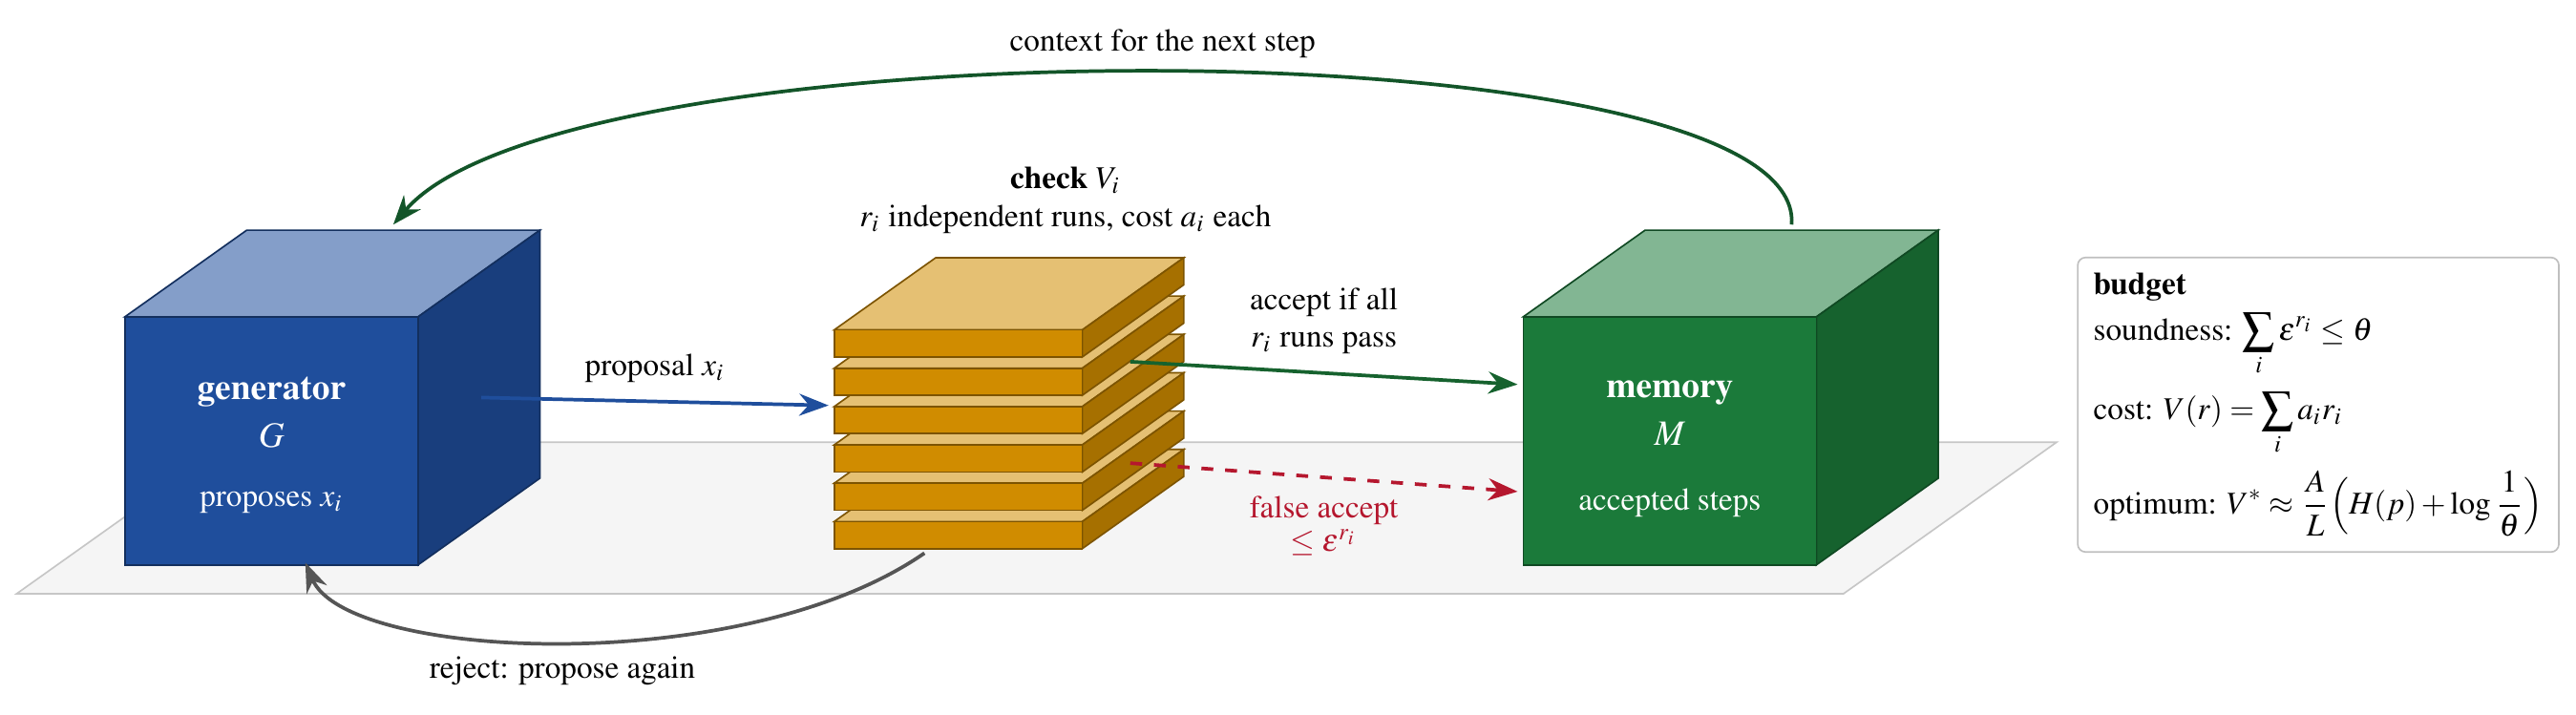
\includegraphics[width=0.94\textwidth]{figures/fig_architecture}
\Description{Block diagram: a generator sends candidate modifications to a bank of checks; accepted candidates enter the system and the cost of all runs is charged to one budget.}
\caption{A BLLM. The generator proposes candidate modifications; the $i$-th candidate is tested by $r_{i}$ independent runs of a check $V_{i}$ of cost $a_{i}$ per run; an incorrect candidate survives all runs with probability at most $\eps^{r_{i}}$ and a correct one always survives; the memory keeps what survives and feeds it back as context. The budget box states the two quantities the paper controls, the expected number of false acceptances $\sum_{i}\eps^{r_{i}}\le\theta$ and the cost $V(r)=\sum_{i}a_{i}r_{i}$, and the value of the optimum (Theorem~\ref{thm:A}).}
\label{fig:architecture}
\end{figure*}

\subsection{What the title means}

The title names two properties, and each is a measured quantity of the system we built, which we call Anaxia (Section~\ref{sec:network}).

\emph{Beyond the LLM} means that a language model, where one is used at all, only proposes. Whether a proposal is kept is decided by checks whose error is priced by the laws of this paper, and every object that the engine keeps from a search is checked again by code that shares nothing with the search. A language model that writes an answer and grades it with the same weights is the case these laws exclude: its check is not independent of its proposal, so the runs of the model have no soundness to spend.

\emph{Deep Human-Mind-AI} means three things, each of which we measure and none of which says that the engine thinks as a person does.
\begin{enumerate}[label=(\alph*),leftmargin=1.8em,itemsep=1pt]
\item \emph{Proposals distributed as people distribute them.} On the axis of research opportunities of \cite{CZC26} the least expected number of proposals per problem is $6.50$; the profile of the human authors pays $7.00$, a factor $1.08$, and the nine language models measured pay between $1.51$ and $4.28$ times the optimum (Table~\ref{tab:gap}). The selector of the engine learns the profile that attains the optimum from the results its checks keep.
\item \emph{Human constructions as the raw material.} The default proposer is not a model but a typed crossing of constructions that mathematicians wrote down, each kept with its provenance, its type and the types it needs, so that a new candidate is a composite of known pieces that fit.
\item \emph{Construction by hand, mechanised.} Construction mode writes down a new object together with the argument for what it forces, as a combinatorialist builds a gadget, and keeps it only after an independent check. From the rules of Steinberg's problem alone it rebuilt the gadgets of the counterexample of Cohen-Addad, Hebdige, Kr\'al', Li and Salgado \cite{CHK17}.
\end{enumerate}

\subsection{The entropy law}

Write $A=\sum_{i}a_{i}$ for the total cost of one run of every check, $p_{i}=a_{i}/A$ for the cost profile, $H(p)=\sum_{i}p_{i}\log(1/p_{i})$ for its entropy, and $L=\log(1/\eps)$. The schedule $r$ is \emph{$\theta$-sound} when the expected number of incorrect candidates kept is at most $\theta$ in every assignment of correct and incorrect candidates, which for checks whose soundness $\eps$ is attained is the inequality $\sum_{i}\eps^{r_{i}}\le\theta$ (Section~\ref{sec:model}). Its cost is $V(r)=\sum_{i}a_{i}r_{i}$, the cost of certifying a run in which every candidate is correct, and $\Vs(\theta)$ is the least cost of a $\theta$-sound schedule.

\begin{mainthm}[Entropy law]\label{thm:A}
For $0<\theta\le1$,
\begin{equation}\label{eq:entropylaw}
\frac{A}{L}\Bigl(H(p)+\log\frac1\theta\Bigr)\ \le\ \Vs(\theta)\ \le\ \frac{A}{L}\Bigl(H(p)+\log\frac1\theta\Bigr)+A .
\end{equation}
The lower bound is attained when every $\theta p_{i}$ is an integer power of $\eps$, and the additive constant $A$ cannot be replaced by $cA$ with $c<1$. The same bounds hold for infinitely many candidates with $A<\infty$, and for schedules drawn at random independently of the checks.
\end{mainthm}

The law says that the price of soundness is an entropy. Certifying $n$ candidates of equal cost costs $(n/L)\log(n/\theta)$ up to $n$, so the tax per candidate grows like $\log n$ and not like a constant: a system that keeps more modifications must test each one harder. A skewed profile is cheaper than a flat one with the same total, because the expensive checks may be run fewer times and the cheap ones more, and the saving is measured exactly by $\log n-H(p)$. The schedule that attains the bound runs the $i$-th check $\lceil\log(A/(\theta a_{i}))/L\rceil$ times, so it spends $\log(1/p_{i})$ nats of soundness on a candidate of relative cost $p_{i}$: this is Shannon's code length \cite{Sha48}, and the analogy is exact.

\begin{mainthm}[Huffman schedules]\label{thm:C}
If $\eps=1/D$ for an integer $D\ge2$ and $\theta=D^{-k}$ for an integer $k\ge0$, then the $\theta$-sound schedules are exactly $r_{i}=\ell_{i}+k$ with $(\ell_{i})$ the lengths of a $D$-ary prefix code, and $\Vs(\theta)=A\bigl(k+L_{D}(p)\bigr)$, where $L_{D}(p)$ is the expected length of a Huffman code for $p$.
\end{mainthm}

So the optimal schedule is computed by Huffman's algorithm \cite{Huf52}, and Kraft's inequality \cite{Kra49,McM56} is the soundness condition in disguise. The additive constant of Theorem~\ref{thm:A} is the redundancy of the Huffman code, which lies in $[0,1)$ in units of $\log D$ \cite{CT06,Gal78}.

Not every check is repeated. A statistical check that averages $m$ samples and accepts when the average is close to its target has false acceptance probability of order $1/m$ by Chebyshev's inequality, not $\eps^{m}$. For a check whose cost to reach false acceptance probability $\delta$ is $a\delta^{-s}$ the entropy is replaced by a R\'enyi entropy \cite{Ren61}.

\begin{mainthm}[R\'enyi law]\label{thm:D}
For checks of polynomial order $s>0$ and $0<\theta\le1$, the least cost of a $\theta$-sound allocation is
\begin{equation}\label{eq:renyilaw}
\Vs_{s}(\theta)=\theta^{-s}\Bigl(\sum_{i}a_{i}^{1/(1+s)}\Bigr)^{1+s}=A\,\theta^{-s}e^{sH_{\alpha}(p)},
\end{equation}
where $\alpha=1/(1+s)$ and $H_{\alpha}$ is the R\'enyi entropy of order $\alpha$; and $\Vs_{s}(\theta)=A\bigl(1+s(H(p)+\log\frac1\theta)\bigr)+O(s^{2})$ as $s\to0$.
\end{mainthm}

The first-order term at $s=0$ is the entropy law, so the R\'enyi law is a one-parameter deformation of it, as Campbell's coding theorem is a deformation of Shannon's \cite{Cam65}. Section~\ref{sec:renyi} also gives a criterion, valid for every cost function, for an infinite sequence of candidates to admit a sound schedule of finite cost.

\subsection{Chains, gates and singularities}

Section~\ref{sec:chains} puts the checks into a self-improvement chain in which the generator retries a step until a candidate is kept. When each step is wrong with probability between $\rho_{\ast}>0$ and $\bar\rho<1$, the least expected cost of the chain with at most $\theta$ expected false acceptances is pinched between the entropy law at budget $\theta/\rho_{\ast}$ and the entropy law at budget $\theta(1-\bar\rho)/\bar\rho$, divided by $1-\bar\rho$ (Theorem~\ref{thm:B}). The same section proves an exponential separation between checking every step and checking only the outcome: with perfect checks the ratio of expected costs is $(1-\rho)^{-(n-1)}\ge e^{(n-1)\rho}$, and with imperfect checks the step check may accept an incorrect step with probability of order $1/n$ while the outcome check must do so with probability exponentially small in $n$ (Theorem~\ref{thm:gating}).

An infinite chain whose total expected cost is finite completes infinitely many improvements in finite cost, and we call it \emph{singular}, after the vertical asymptote of the explosion literature. It is \emph{sound} when the number $F$ of incorrect modifications it keeps is finite.

\begin{mainthm}[Sound singularities]\label{thm:E}
Let the $n$-th step cost $g_{n}$ to generate and $a_{n}\le1$ per run to check, with error probabilities in $[\rho_{\ast},\bar\rho]\subset(0,1)$, independent steps and checks of exact soundness $\eps$. Then
\begin{enumerate}[label=\textup{(\roman*)},leftmargin=2.2em,itemsep=1pt]
\item $F<\infty$ almost surely, or $\PR(F=0)>0$, if and only if $\sum_{n}\eps^{r_{n}}<\infty$, and otherwise $F=\infty$ almost surely;
\item a singular chain in which every step is checked exists if and only if $\sum_{n}g_{n}<\infty$ and $\sum_{n}a_{n}<\infty$;
\item a sound singular chain exists if and only if in addition $\sum_{n}a_{n}\log(1/a_{n})<\infty$.
\end{enumerate}
\end{mainthm}

So there is a soundness gap. For $a_{n}=1/(n\log^{\beta}n)$ a singular chain exists for every $\beta>1$, and a sound one only for $\beta>2$; between the two, every schedule fast enough to reach the asymptote keeps infinitely many errors almost surely (Corollary~\ref{cor:gap}). For a power law $a_{n}=n^{-p}$ the price of soundness, the ratio of the cheapest sound cost to the cost of one run per step, is $1/((p-1)L)+O(\log\frac1{p-1})$, and with polynomial checks of order $s$ a sound singularity exists exactly when $p>1+s$ (Fig.~\ref{fig:regimes}).

When the improvements branch, each kept improvement spawning a random number of candidates, the process is a Galton--Watson tree \cite{WG75,AN72}.

\begin{mainthm}[Branching takeoff]\label{thm:F}
Let $m$ be the mean number of correct offspring kept per kept improvement, and let the check of generation $k$ accept an incorrect candidate with probability $\delta_{k}$. Then the takeoff survives with positive probability if and only if $m>1$; the expected number of kept errors is $\mu(1-\gamma)\sum_{k\ge1}m^{k-1}\delta_{k}$; and if this series diverges then, under $\EE\,\xi\log\xi<\infty$, infinitely many errors are kept almost surely on survival. With exponential checks, soundness forces $r_{k}\ge k\log m/L$ for all large $k$, and $r_{k}=\lceil k\log(2m)/L\rceil$ suffices.
\end{mainthm}

Here $\mu$ is the mean number of candidates per kept improvement, $\gamma$ the probability that a candidate is correct and $\xi$ the number of candidates. A fixed false acceptance rate, however small, is fatal to an explosive takeoff, and the number of runs per check must grow linearly in the generation, that is, logarithmically in the size of the population: the entropy tax again.

\subsection{Without foresight, among many agents}

The schedules above are computed from the whole cost profile. A system that improves itself does not know its future candidates: when the $n$-th one arrives, only $a_{1},\dots,a_{n}$ are known, and the runs of its check must be fixed then. Theorem~\ref{thm:G} gives a rule that uses only the running total $S_{n}=a_{1}+\dots+a_{n}$, is $\theta$-sound for every sequence of costs, and pays over the offline optimum at most $\frac{A_{N}}{L}\bigl(\log2+2\log(1+\log\frac{A_{N}}{a_{1}})\bigr)+A_{N}$ on the first $N$ candidates; on the doubling costs every online rule pays an excess of order $\frac{A_{N}}{L}\log\log\frac{A_{N}}{a_{1}}$, so the double logarithm is the true price of not knowing the future (Fig.~\ref{fig:online}). Consequently the criterion of Theorem~\ref{thm:E} needs no oracle: a chain that knows only its past reaches a sound singularity whenever any chain does (Corollary~\ref{cor:onlinesing}).

A working system also delegates. When a coordinator splits the candidates among subagents, the entropy satisfies the chain rule over the split, and Theorem~\ref{thm:H} shows that a coordinator which gives each subagent the share of the budget proportional to its total cost loses nothing: each subagent, knowing only its own costs and one number, computes on its candidates exactly the optimal schedule of the whole system, and along a tree of delegation the entropy tax is paid node by node. Any other split costs exactly $\frac AL$ times a Kullback--Leibler divergence. Finally, cheap checks of soundness $\eps$ placed before one exact check of cost $c$ make the exact check paid only on the correct candidates, with a premium $\frac bL(1+\log\frac{c\rho L}{b})$ logarithmic in the ratio of costs (Theorem~\ref{thm:cascade}). These two results are the laws of the system of subagents built in Section~\ref{sec:agents}; Appendix~\ref{sec:cases} reads six machine-checked or published proofs of hard problems in their terms.

\subsection{The gap between human and LLM thinking}

Let a problem need an idea of class $j$ with probability $\pi_{j}$, and let a proposer draw classes from a profile $q$ until it draws the needed one. The expected number of proposals is $\sum_{j}\pi_{j}/q_{j}$, and Theorem~\ref{thm:I} shows that it is at least $e^{H_{1/2}(\pi)}=(\sum_{j}\sqrt{\pi_{j}})^{2}$, a R\'enyi entropy of order one half, attained only by square-root sampling; the excess is exactly $e^{H_{1/2}(\pi)}$ times the chi-squared divergence of $q$ from square-root sampling, and mixing a fraction $\lambda$ of square-root sampling into any proposer brings its cost under $e^{H_{1/2}(\pi)}/\lambda$. On the data of \cite{CZC26} the optimum is $6.50$ proposals per problem on the axis of research opportunities and $6.45$ on the axis of methods; the human profile itself pays $7.00$, and the nine models pay from $1.51$ to $4.28$ times the optimum (Table~\ref{tab:gap}). A BLLM learns the need from the results its checks keep, and its excess over the optimum falls like $\beta(\pi)/(4n)$ after $n$ closed problems (Proposition~\ref{prop:learnrate}), for a constant $\beta(\pi)$ that is $7.06$ on the human profile of opportunities. The learning is done by a race of leaky integrate-and-fire neurons with a reward-modulated synapse, which samples exactly the square root of the counts it has learned (Proposition~\ref{prop:spiking}). Appendix~\ref{sec:brains} sets this circuit beside three wiring diagrams measured synapse by synapse, of the worm \textit{C.~elegans}, of the fly \textit{Drosophila} and of a cubic millimetre of human cortex, and computes from them the sensory-to-motor depth, the modular structure and the laminar composition that the three parts of a BLLM reproduce.

\subsection{Towers}

An engine can act on another engine: one that chooses among strategies of a proposer and keeps the strategies that work stands on the proposer, and one that runs several copies of it and keeps the better half stands on that. Section~\ref{sec:towers} prices such a tower. If $n$ verified layers share a budget $\theta$ of false acceptances, because a false acceptance low in the tower contaminates everything above it, then certifying the tower costs at least $n\log(n/\theta)$ nats of soundness, each added layer raises the bound by at least $\log((n+1)/\theta)$, and past a finite depth every tower costs more than any fixed amount (Theorem~\ref{thm:tower}). Depth pays only while it lowers the search by more than the increment, and the theorem says that this stops.

\subsection{The engine and what it did}

The theorems price the checks; they do not say where good candidates come from. Section~\ref{sec:network} describes the engine and Sections~\ref{sec:experiments} to~\ref{sec:hodgeround} measure it. Known constructions are typed nodes, each with the type of object it gives and the types it needs; a candidate is a cross that fills an input of one construction with the output of another; every closed cross is checked by a program, attacked by a refuter, and recorded in a shared memory. A target point fixes for each problem the statement that would settle it, five agents, one per problem, attack through a channel that brings every relevant record of the memory to the proposer, and construction mode builds new objects where crossing has nothing to combine. We ran the engine on five open problems, the lattice mass gap of Yang--Mills theory, the Hodge conjecture, Grothendieck's standard conjecture of Lefschetz type, Chowla's conjecture and Erd\H{o}s problem 1183, on Steinberg's problem as a calibration, and on two conjectures from mathematical physics. The measurements are these.
\begin{enumerate}[label=(\roman*),leftmargin=1.8em,itemsep=1pt]
\item \emph{Typing does the work.} On Yang--Mills the network reached in every run a composite whose check accepts a lattice mass gap for four-dimensional $\mathrm{SU}(2)$ on $\beta_{W}<\frac13$, which no run of random or type-filtered pairing reached; random pairing wastes $45$ of $48$ crosses on ill-typed pairs. The composite was first proposed by the language-model proposer and then entered in the library, so the network reproduces the step rather than originating it. The step itself, Theorem~\ref{thm:onethird}, is proved here and has not been refereed; it extends the range $\beta_{W}<\frac29$ of \cite{BB26d}, and Proposition~\ref{prop:forestceiling} shows that $\frac13$ is the ceiling of the method.
\item \emph{Boosters do not help.} Hebbian weights with path credit reached that step in $12$ and $14$ of $200$ runs against $21$ for the unboosted network, a difference within two standard errors; a booster strengthens synapses that have fired, and the step needed one that had not.
\item \emph{Memory halves the cost.} Over $60$ seeds and five rounds the full system reaches its plateau of about six survivors with $46.4$ checks against $95.2$ without memory, because it never checks a decided composite twice; it does not raise the plateau.
\item \emph{Agents are cheaper and reach no further.} After eleven rounds the five agents hold $24$ distinct survivors for $250$ checks and a single loop $27$ for $797$; the agents level off in the second round, the loop passes them in the sixth with known results, and no survivor of either reaches a target point.
\item \emph{Patterns transfer partially or fail.} Of $38$ transfers of a pattern that broke a comparable barrier elsewhere to a blocking step, none closes, $7$ give a weaker statement or a new computation and $31$ fail, for one of three reasons recorded in Section~\ref{ssec:matrix}.
\item \emph{Construction mode rebuilds what crossing cannot.} Random planar frames filled with library gadgets gave no gadget of Steinberg's kind in $2.45$ million frames; the goal-directed builder, given only the rules, rebuilt the $15$-vertex gadget of \cite{CHK17} on its $116$th try after $11$ seconds. With that gadget and a triangle as lemmas it built a $42$-vertex gadget with the contacts of the second gadget of \cite{CHK17} on two seeds, and on a third a $48$-vertex gadget with contact distances $5,4,5$, which \cite{CHK17} does not use, and the assembly of \cite{CHK17} applied to the rebuilt $15$-vertex gadget gives a planar graph of $166$ vertices with no cycle of length $4$ or $5$ that three satisfiability solvers find not $3$-colourable. On Erd\H{o}s's question, which also forbids cycles of length $6$, it finds nothing (Section~\ref{ssec:steinberg}).
\item \emph{Depth pays once.} At equal budgets of exact checks, a second layer that first builds an easier gadget and keeps it as a lemma reaches the profile of the second gadget of \cite{CHK17} on seven of ten runs, where the builder alone never reaches it; a third layer reaches it on six. When all layers share one library and one set of weights, the step from the lemma to the goal takes a median of $308$ checks against $2{,}342$ when each copy keeps its own. The crossing loop, given $13$ to $20$ times the budget, finds no gadget, and no tower finds one on Erd\H{o}s's question (Section~\ref{ssec:towerbench}).
\item \emph{One problem only.} Pointed at the Hodge conjecture alone, with every result of \cite{BB26c} and of the companion paper \cite{BMB26b} in its library, the engine excludes by counting two of the configurations left open on $E_{0}^{6}$, a parity count on the closed chains against the Chern character excludes a third up to seven line bundles at every discriminant, the fourth reduces to the ranks of explicit Massey products, and the gap of every target point is the same after the last round as after the first (Section~\ref{sec:hodgeround}).
\item \emph{It learns from its failures.} Every failed attempt writes a record that names the part that failed, changes one rule of the engine and is closed by the outcome of the next attempt under the changed rule. In the log so far, \modChanges{} changes of rule followed \modAttempts{} attempts on \modTargets{} targets, and of the \modBuilt{} changes that were built, \modRetryClosed{} led to a retry that closed its target and \modRetryPartial{} more to one that moved it forward. The loop never makes the same change twice on a target, so it stops after at most one attempt more than there are changes it can propose (Proposition~\ref{prop:loopstops}), and it ranks the kinds of change by the posterior mean of their success (Proposition~\ref{prop:playbook}); Section~\ref{sec:selfmod}.
\item \emph{A benchmark crossed.} On a conjecture about the reflexive polytopes of dimension four, whose Calabi--Yau hypersurfaces form the largest known list of Calabi--Yau threefolds, the engine reached a proof: shrunk one reflexive polytope at a time, such a polytope reaches a seed in at most $\seedBound$ steps, for all $\seedCount$ polytopes of the Kreuzer--Skarke list, because each step lowers the number of lattice points of the polytope and raises that of its dual (Theorem~\ref{thm:seedbound}). In dimensions two and three the sharp constants are $\seedTwo$ and $\seedThree$; in dimension four the sharp constant lies between $\seedLow$ and $\seedBound$ and is open. This passes the sixth benchmark, one open conjecture of mathematical physics proved without conditions (Section~\ref{sec:seed}).
\end{enumerate}
On Erd\H{o}s problem 1183 a reduction to weighted posets (Lemma~\ref{lem:levelposet}) gives the upper bounds that, with the known lower bounds, determine $f(n)$ for $n\le20$ (Theorem~\ref{thm:fvalues}). None of the five problems is solved, and Section~\ref{ssec:whyhard} states for each the step at which every construction we hold stops; the sixth benchmark is passed, by the seed conjecture.

\subsection{What the paper proves}

Table~\ref{tab:results} lists the results. The proofs are complete and elementary: the entropy law rests on the inequality $\log x\le x-1$, the R\'enyi law on H\"older's inequality, the singularity theorem on the Borel--Cantelli lemmas, the online law on a telescoping inequality for $\log(S_{n}/a_{1})$, the branching theorem on the Kesten--Stigum theorem \cite{KS66} and L\'evy's conditional form of the Borel--Cantelli lemma \cite{Dur19}, and the tower law on the entropy law with unit costs. Every finite inequality, the online and subagent laws, the gap law, the cascade bounds, the Kraft--schedule correspondence, the R\'enyi optimum, the convergence criteria for sound schedules, both Borel--Cantelli statements and the tower law are proved in Lean~4 with Mathlib, in sixty-five theorems that depend only on the three standard axioms (Appendix~\ref{app:checks}); the probabilistic limit theorems and the asymptotics of the zeta function are proved in the text and are not formalised.

The paper does not prove that any existing system is sound, and it does not predict whether an intelligence explosion will happen. Its theorems are conditional on a model, stated in Section~\ref{sec:model}: independent runs, perfect completeness, and schedules fixed in advance. Remark~\ref{rem:adaptive} shows that the last assumption matters, since a schedule allowed to stop at the first detected error escapes the entropy term at the price of discarding good work. What the paper does establish is that, inside the model, the cost of soundness is computable in closed form, that it is an entropy, and that it separates the singular processes into sound and unsound ones by a single convergent series.

\begin{table*}[t]
\caption{The main results. $A=\sum a_{i}$, $p=a/A$, $L=\log(1/\eps)$; ``Lean'' names the formalised statements of Appendix~\ref{app:checks}.}
\label{tab:results}
\centering
\footnotesize
\setlength{\tabcolsep}{4pt}
\begin{tabular}{@{}p{0.13\textwidth}p{0.36\textwidth}p{0.13\textwidth}p{0.32\textwidth}@{}}
\toprule
\rr Result & \rr Statement & \rr Proof & \rr Lean \\
\midrule
\rr Theorem~\ref{thm:A} & \rr $\frac AL(H+\log\frac1\theta)\le \Vs(\theta)\le \frac AL(H+\log\frac1\theta)+A$ & \rr Gibbs, ceilings & \rr \lean{verification\_lower}, \lean{ceilSchedule\_cost} \\
\rr Proposition~\ref{prop:clean} & \rr clean runs: budgets $\theta$ and $\log\frac1{1-\theta}$ & \rr $1-\sum q\le\prod(1-q)\le e^{-\sum q}$ & \rr \lean{clean\_ge}, \lean{clean\_budget} \\
\rr Proposition~\ref{prop:random} & \rr random oblivious schedules obey Theorem~\ref{thm:A} & \rr Jensen & \rr \lean{randomised\_budget} \\
\rr Proposition~\ref{prop:twosided} & \rr two-sided checks, rate $\frac12\log\frac1{4q(1-q)}$ & \rr Chernoff & \rr --- \\
\rr Theorem~\ref{thm:C} & \rr $\Vs(D^{-k})=A(k+L_{D}(p))$ & \rr Kraft, Huffman & \rr \lean{kraft\_of\_schedule}, \lean{schedule\_of\_kraft} \\
\rr Theorem~\ref{thm:D} & \rr $\Vs_{s}(\theta)=A\theta^{-s}e^{sH_{1/(1+s)}(p)}$ & \rr H\"older & \rr \lean{renyi\_lower}, \lean{renyi\_attain} \\
\rr Theorem~\ref{thm:dual} & \rr sound schedule $\iff\sum a_{n}\psi(\lambda/a_{n})<\infty$ & \rr Legendre duality & \rr \lean{schedule\_of\_dual\_summable} \\
\rr Theorem~\ref{thm:B} & \rr chain cost between two entropy laws & \rr Wald & \rr \lean{entropy\_lower}, \lean{ceilSchedule\_sound} \\
\rr Theorem~\ref{thm:gating} & \rr step versus outcome checks: $(1-\rho)^{-(n-1)}$ & \rr products & \rr \lean{separation}, \lean{precision\_bounds} \\
\rr Theorem~\ref{thm:E} & \rr sound singularity $\iff\sum g,\sum a,\sum a\log\frac1a<\infty$ & \rr Borel--Cantelli & \rr \lean{sound\_schedule\_iff}, \lean{false\_accepts\_infinite} \\
\rr Corollary~\ref{cor:gap} & \rr soundness gap $1<\beta\le2$ & \rr condensation & \rr --- \\
\rr Proposition~\ref{prop:powerlaw} & \rr price $\sim1/((p-1)L)$ for $a_{n}=n^{-p}$ & \rr integral comparison & \rr --- \\
\rr Proposition~\ref{prop:osgood} & \rr Osgood takeoff: check time $\asymp\kappa/(c(\alpha-1)^{2}L)$ & \rr entropy of $\zeta$ & \rr --- \\
\rr Theorem~\ref{thm:G} & \rr online rule: excess $\le\frac{A_{N}}L(\log2+2\log(1+\log\frac{A_{N}}{a_{1}}))+A_{N}$ & \rr telescoping & \rr \lean{onlineSchedule\_sound}, \lean{online\_lower} \\
\rr Theorem~\ref{thm:H} & \rr split price $\frac AL(D(P\|q)+\log\frac\theta\Theta)$ & \rr chain rule & \rr \lean{chain\_rule}, \lean{split\_lower}, \lean{proportional\_split} \\
\rr Theorem~\ref{thm:cascade} & \rr cascade: $\min E=c(1-\rho)+\frac bL(1+\log\frac{c\rho L}b)+O(b)$ & \rr $\log x\le x-1$ & \rr \lean{cascade\_lower}, \lean{cascade\_upper} \\
\rr Theorem~\ref{thm:F} & \rr branching takeoff and $r_{k}\ge k\log m/L$ & \rr Kesten--Stigum, L\'evy & \rr \lean{amplified\_summable}, \lean{contamination\_diverges} \\
\rr Theorem~\ref{thm:tower} & \rr $n$ layers: $\sum_{k}\log\frac1{\beta_{k}}\ge n\log\frac n\theta$; saturation & \rr Theorem~\ref{thm:A}, unit costs & \rr \lean{tower\_cost\_lower}, \lean{tower\_saturates} \\
\rr Theorem~\ref{thm:I} & \rr proposals $\sum\pi_{j}/q_{j}\ge e^{H_{1/2}(\pi)}$, excess $e^{H_{1/2}}\chi^{2}(r\|q)$ & \rr Cauchy--Schwarz & \rr \lean{search\_lower}, \lean{search\_chi2}, \lean{search\_mix} \\
\rr Proposition~\ref{prop:learnrate} & \rr learned square-root sampling: $1+\beta(\pi)/(4n)$ & \rr second-order expansion & \rr --- \\
\rr Proposition~\ref{prop:spiking} & \rr first spike of the race is $\sqrt{c_{k}+\alpha}/\sum_{l}\sqrt{c_{l}+\alpha}$ & \rr exponential race & \rr --- \\
\rr Lemma~\ref{lem:depth} & \rr processing depth of a wiring diagram & \rr Laplacian & \rr --- \\
\bottomrule
\end{tabular}
\end{table*}

\subsection{Organisation}

Section~\ref{sec:history} traces the lines that meet here: self-reference and the intelligence explosion, coding and testing, branching processes, and verifiers for language models; Section~\ref{sec:related} sets the engine beside the systems that search against an evaluator, FunSearch, AlphaEvolve, AlphaProof and the provers trained against Lean, and says what is taken from each and what is not. Section~\ref{sec:model} defines the model. Sections~\ref{sec:entropy} to~\ref{sec:renyi} prove the entropy law, its Huffman form and its R\'enyi deformation. Section~\ref{sec:chains} treats chains and the comparison of step and outcome checks, Section~\ref{sec:singularity} singular chains, Section~\ref{sec:online} the online law, Section~\ref{sec:agents} subagents and cascades, Section~\ref{sec:gap} the gap between human and model proposals and the spiking selector that closes it, Section~\ref{sec:branching} the branching takeoff and Section~\ref{sec:towers} towers of verified layers. Section~\ref{sec:network} describes Anaxia, Section~\ref{sec:benchmark} the six benchmarks with their pass lines, Section~\ref{sec:experiments} the measurements of the crossing network, Section~\ref{sec:construct} construction mode and the towers at equal cost, Section~\ref{sec:brain} the anatomy of the engine and how it grew, Section~\ref{sec:selfmod} the loop that learns from failure, Section~\ref{sec:seed} the benchmark it crossed, and Section~\ref{sec:hodgeround} a round on the Hodge conjecture alone. Section~\ref{sec:status} states what is proved and what is open. Appendix~\ref{app:derivations} proves the classical facts used, Appendix~\ref{app:checks} lists the Lean statements and numerical checks, Appendix~\ref{app:hardware} the hardware each part of the engine needs, Appendix~\ref{app:sources} the systems and collections it draws on, and the last three appendices set the selector beside three measured nervous systems, relate the cost sequences to growth and scaling laws, and read six formal proofs of hard problems in the language of the paper.

Logarithms are natural unless a base is shown; $\NN=\{0,1,2,\dots\}$.

\section{History}\label{sec:history}

Three lines of work meet in this paper, and a fourth, recent one supplies its motivation. Figure~\ref{fig:history} places them on one time axis and Table~\ref{tab:history} lists what each contributes to the argument.

\begin{figure*}[t]
\centering
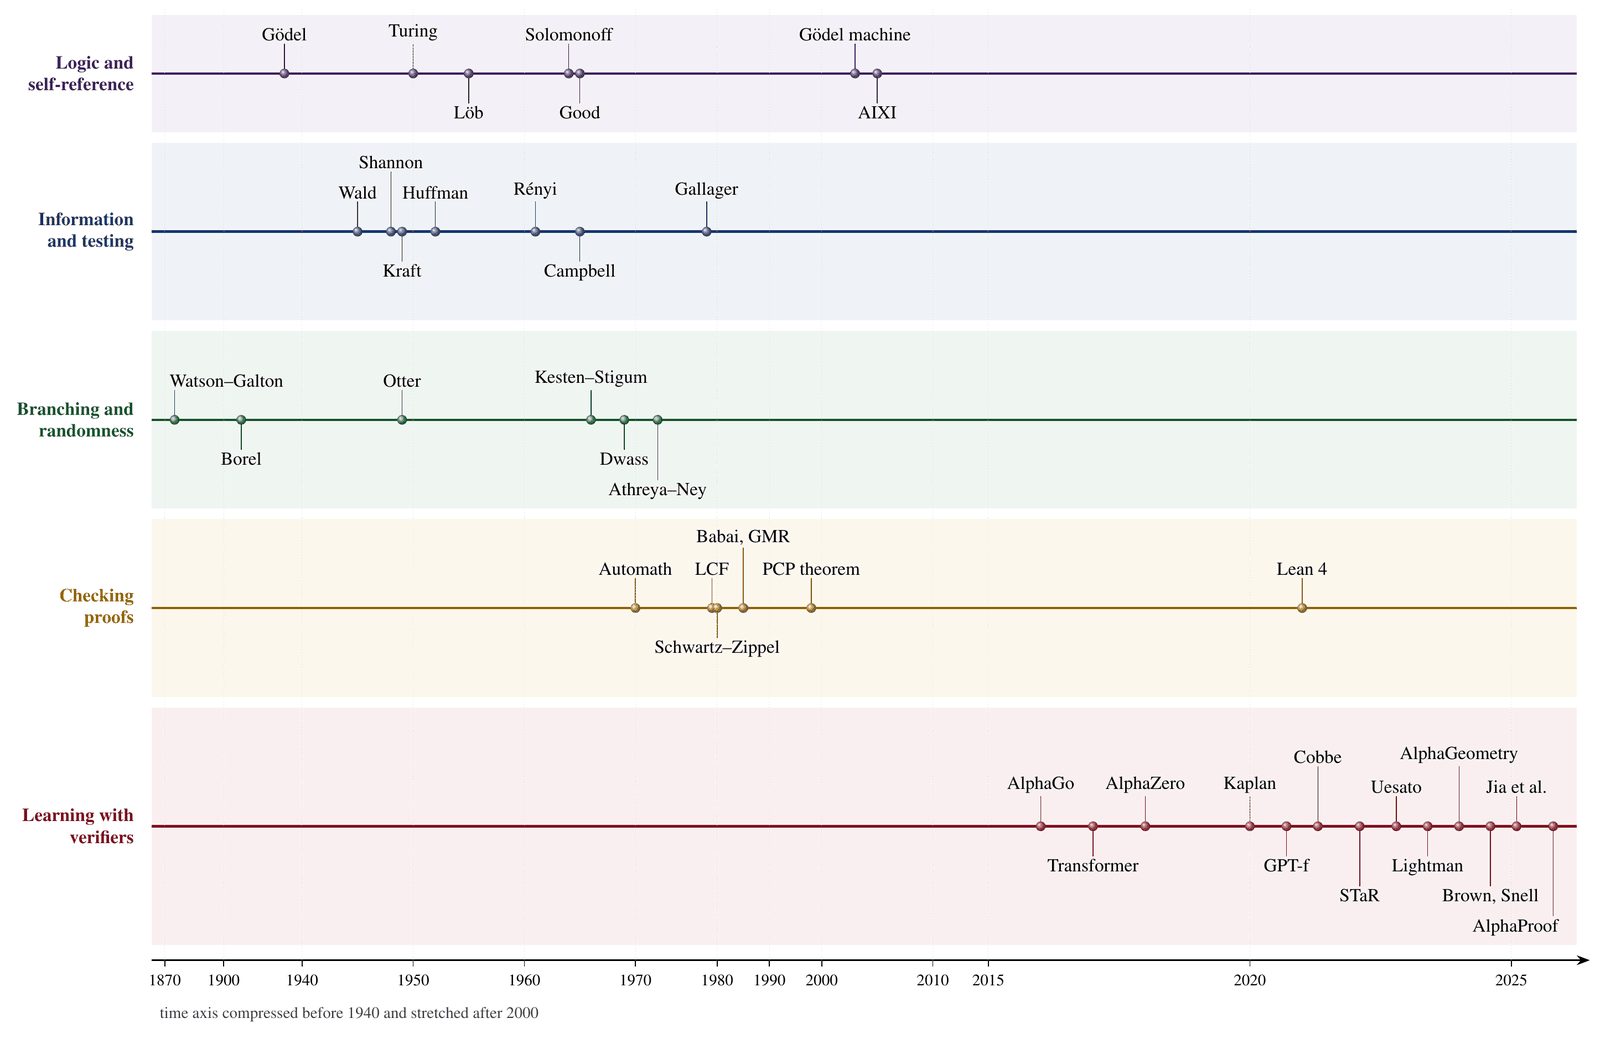
\includegraphics[width=\textwidth]{figures/fig_history}
\caption{Five lines of work on one time axis, with the scale stretched after 2015. Logic and self-reference: G\"odel's incompleteness theorems, Turing's learning machine, L\"ob's theorem, Solomonoff's induction, Good's intelligence explosion, the G\"odel machine and AIXI. Information and testing: Wald's sequential tests, Shannon's source coding, Kraft's inequality, Huffman's codes, R\'enyi's entropies, Campbell's coding theorem and Gallager's redundancy bound. Branching and randomness: the Watson--Galton problem, Borel's denumerable probabilities, Otter's multiplicative process, the Kesten--Stigum theorem, Dwass's total progeny and the monograph of Athreya and Ney. Checking proofs: Automath, LCF, the polynomial identity test of Schwartz and Zippel, interactive proofs, the PCP theorem and Lean~4. Learning with verifiers: from AlphaGo and the transformer to trained verifiers, process supervision, repeated sampling and AlphaProof.}
\label{fig:history}
\end{figure*}

\subsection{Self-reference and the intelligence explosion}

Turing's paper of 1950 already contains the idea of a machine that improves itself: rather than program an adult mind, one should program a child machine and educate it, and he expected the educated machine to be modified by its own experience \cite{Tur50}. Fifteen years later Good drew the consequence for machines better than their designers \cite{Goo66}. The formal theory of such machines met an obstacle at once, and the obstacle is logical. G\"odel's second incompleteness theorem shows that a consistent system containing arithmetic does not prove its own consistency \cite{God31}, and L\"ob's theorem sharpens it: if such a system proves that provability of a sentence implies the sentence, then it proves the sentence \cite{Lob55}.\footnote{L\"ob's theorem answers a question of Henkin. Let $T$ be a consistent recursively axiomatised extension of Peano arithmetic and $\mathrm{Prov}_{T}$ its provability predicate. If $T\vdash\mathrm{Prov}_{T}(\ulcorner\varphi\urcorner)\to\varphi$ then $T\vdash\varphi$. Applied to a self-modifying agent that keeps a successor only when it proves the successor sound, the theorem forbids the agent from accepting, in general, a successor that uses the same proof system with the same trust, since that acceptance would require the agent to prove a reflection principle for its own system. The present paper avoids the obstacle by replacing proofs of soundness with randomized checks of bounded error, whose reliability is a probability, not a theorem of the system.} An agent that rewrites itself only after proving that the rewrite is sound cannot in general accept a successor as strong as itself. Schmidhuber's G\"odel machine makes this precise in the other direction: it rewrites any part of its own code once it has found a proof that the rewrite increases expected utility, and is optimal among such strategies relative to its axioms \cite{Sch03}. Solomonoff's theory of inductive inference \cite{Sol64} and Hutter's AIXI \cite{Hut05} give the ideal, uncomputable agents against which the practical ones are measured.

The present paper does not ask for proofs. It asks for checks with a stated probability of error and counts what they cost. That shift, from certainty to bounded error, is the one complexity theory made between the 1970s and the 1990s.

\subsection{Coding and testing}

Shannon's theorem of 1948 says that a source with distribution $p$ cannot be encoded by a uniquely decodable code in fewer than $H(p)$ symbols on average, and that $H(p)+1$ can be reached \cite{Sha48}. Kraft's inequality, from his master's thesis of 1949, characterises the lengths of prefix codes \cite{Kra49}; McMillan extended it to all uniquely decodable codes \cite{McM56}; Huffman's algorithm of 1952 finds an optimal code \cite{Huf52}; Gallager bounded its redundancy \cite{Gal78}. R\'enyi introduced in 1961 a family of entropies $H_{\alpha}$ that share the additivity of Shannon's \cite{Ren61}, and Campbell showed in 1965 that $H_{\alpha}$ is the optimal mean length when long codewords are penalised exponentially \cite{Cam65}. The standard account is \cite{CT06}.

The connection with checking is older than it looks. Wald's sequential tests of 1945 already treat the trade-off between the number of observations and the two probabilities of error \cite{Wal45}, and Chernoff's exponent of 1952 \cite{Che52} and Hoeffding's inequality of 1963 \cite{Hoe63} give the rates at which repeated observations drive the error down. What seems not to have been noticed is that the optimal allocation of repetitions among many checks of unequal cost under a common error budget is a coding problem, with costs in the role of probabilities and repetitions in the role of codeword lengths. Theorems~\ref{thm:A} and~\ref{thm:C} make the identification exact.

\subsection{Branching and randomness}

The Watson--Galton paper of 1875 asked for the probability that a surname dies out, and reduced the question to the iteration of a generating function \cite{WG75}; the conclusion drawn there, that every family dies out, was wrong, and the correct criterion, extinction with probability one exactly when the mean number of sons is at most one, became standard only in the twentieth century. Otter's multiplicative process of 1949 put the theory in its modern form \cite{Ott49}, Kesten and Stigum proved in 1966 that the normalised population converges to a limit that is positive on survival exactly when $\EE\,\xi\log\xi<\infty$ \cite{KS66}, and Dwass related the total progeny to a random walk \cite{Dwa69}; the monograph of Athreya and Ney is the reference \cite{AN72}. Borel's paper of 1909 on denumerable probabilities contains the first form of the Borel--Cantelli lemma \cite{Bor09}, which decides here whether a sound singular chain keeps finitely many errors. Osgood's criterion of 1898 for blow-up of the equation $y'=f(y)$ \cite{Osg98} is the continuous form of the condition $\sum a_{n}<\infty$ for a singularity.

\subsection{Checking proofs}

De Bruijn's Automath \cite{dB70} and Milner's LCF \cite{GMW79} began the mechanical checking of proofs, and Lean~4 \cite{MU21} is the system used here. In parallel, complexity theory replaced certainty by bounded error. Schwartz and Zippel showed that a polynomial identity can be tested by evaluating at random points, with error at most the degree divided by the size of the field per run \cite{Sch80,Zip79}; Babai \cite{Bab85} and Goldwasser, Micali and Rackoff \cite{GMR89} introduced interactive proofs, in which a verifier is convinced with error probability that halves with each round; the PCP theorem showed that every proof can be written so that a verifier reads a constant number of its bits and errs with probability at most one half \cite{AS98,ALM98}. These are exactly the checks of the present paper: perfect completeness, soundness $\eps<1$ per run, and independent repetition.

\subsection{Learning with verifiers}

The fourth line is recent. AlphaGo \cite{SHM16} and AlphaZero \cite{SHS18} learned games by self-play against an exact referee, the rules of the game. Transformers \cite{VSP17} and the scaling of language models \cite{BMR20,KMH20,HBM22} produced generators of proofs and programs, and verifiers were added to them: Polu and Sutskever coupled a language model to the Metamath checker \cite{PS20}, Cobbe and coauthors trained verifiers to rank solutions of arithmetic problems \cite{CKB21}, Uesato and coauthors and Lightman and coauthors compared rewards for the final answer with rewards for every step \cite{UKK22,LKB23}, and chains of thought made the steps explicit \cite{WWS22}. Self-improvement loops followed: a model trained on its own checked rationales \cite{ZWM22}, on its own consistent answers \cite{HGH22}, on its own feedback \cite{MTG23} or on a constitution \cite{BKK22}. Spending computation at inference time, by sampling many candidates and keeping the checked ones, became a lever of its own \cite{BJE24,SLX24}. AlphaGeometry \cite{TWL24} and AlphaProof \cite{HMS25} reached olympiad level by searching against exact checkers. Errors of transformers on compositional tasks grow with the number of steps \cite{DLS23}, which is one reason to check every step. The same division of labour now builds scientific data. The wiring diagram of an adult fruit fly brain, $139{,}255$ neurons and about $5\times10^{7}$ chemical synapses, was segmented automatically from electron micrographs and accepted neuron by neuron after manual proofreading, which took about $33$ person-years \cite{DMS24}.\footnote{S.~Dorkenwald et~al., \emph{Neuronal wiring diagram of an adult brain}, Nature 634 (2024), 124--138, doi:10.1038/s41586-024-07558-y \cite{DMS24}. A further round of proofreading of $826$ central-brain neurons measured the accuracy of the accepted reconstruction at an average $F_{1}$ score of $99.2\%$ by volume. The proofreading is the check of this paper and the person-years are its cost; Theorem~\ref{thm:A} says how such a budget is best divided when neurons differ in size and the tolerated number of accepted errors is fixed.}

The theory has followed. Jia, Rakhlin and Xie showed that learning from outcome supervision is statistically no harder than learning from process supervision, up to polynomial factors in the horizon \cite{JRX25}; Botta and coauthors showed that a process verifier can turn an intractable generation problem into a tractable one \cite{BLM25}; Rohatgi and coauthors showed that small errors of a learned verifier are amplified along a generation and designed a backtracking sampler that resists them \cite{RSS25}; Balcan and coauthors studied learned verifiers of chains of thought and the asymmetric role of their soundness errors \cite{BBF26}; Scrivens reported that classifier-based safety gates fail over many rounds of self-improvement while a verifier with analytic bounds does not \cite{Scr26}; Guo turned impossibility results into design rules \cite{Guo26}; Lu compared improvements of agentic systems through bounded verification and showed that independent majority amplification preserves the languages it defines \cite{Lu26}. On the growth side, Ord showed that singular growth requires the time around the feedback loop to tend to zero \cite{Ord26}, Anbar Jafari, Ozcinar and Anbarjafari gave testable conditions for runaway growth \cite{AOA25}. The verifier-gated engine of \cite{Bha26a}, in which a generator proposes steps toward a proof and a verifier accepts or rejects each one, is the informal model on which the present architecture is built.

None of these works prices soundness. They bound sample complexity, query complexity, error amplification or growth rates, and they treat the verifier as given. The question here is how a fixed budget of false acceptances should be distributed over many checks of different costs, and what that distribution costs; the answer is an entropy, and it decides which singular takeoffs are sound.

\begin{table*}[t]
\caption{Milestones used in the paper. The last column says where each enters the argument.}
\label{tab:history}
\centering
\small
\begin{tabular}{@{}l l p{0.42\textwidth} l@{}}
\toprule
Year & Work & Contribution & Used in \\
\midrule
1875 & Watson, Galton \cite{WG75} & extinction of families by iterating a generating function & Theorem~\ref{thm:F} \\
1898 & Osgood \cite{Osg98} & blow-up of $y'=f(y)$ in finite time & Section~\ref{sec:scaling} \\
1909 & Borel \cite{Bor09} & denumerable probabilities, Borel--Cantelli & Theorem~\ref{thm:E} \\
1931, 1955 & G\"odel, L\"ob \cite{God31,Lob55} & limits of self-trust in formal systems & Section~\ref{sec:history} \\
1945 & Wald \cite{Wal45} & sequential tests and two probabilities of error & Section~\ref{ssec:twosided} \\
1948 & Shannon \cite{Sha48} & entropy as the optimal mean code length & Theorem~\ref{thm:A} \\
1949, 1956 & Kraft, McMillan \cite{Kra49,McM56} & lengths of prefix and decodable codes & Theorem~\ref{thm:C} \\
1949 & Otter \cite{Ott49} & multiplicative processes & Theorem~\ref{thm:F} \\
1952 & Huffman \cite{Huf52} & optimal prefix codes & Theorem~\ref{thm:C} \\
1952 & Chernoff \cite{Che52} & exponential rate of tests on sums & Proposition~\ref{prop:twosided} \\
1961, 1965 & R\'enyi, Campbell \cite{Ren61,Cam65} & entropies of order $\alpha$ and exponential code costs & Theorem~\ref{thm:D} \\
1965 & Good \cite{Goo66} & the intelligence explosion & Section~\ref{sec:intro} \\
1966 & Kesten, Stigum \cite{KS66} & the limit $Z_{k}/m^{k}$ on survival & Theorem~\ref{thm:F} \\
1979--1980 & Schwartz, Zippel \cite{Sch80,Zip79} & randomized identity tests with one-sided error & Section~\ref{sec:model} \\
1985--1998 & Babai; GMR; PCP \cite{Bab85,GMR89,AS98,ALM98} & bounded-error verification of proofs & Section~\ref{sec:model} \\
2003 & Schmidhuber \cite{Sch03} & self-rewriting after a proof of improvement & Section~\ref{sec:history} \\
2021--2023 & Cobbe; Uesato; Lightman \cite{CKB21,UKK22,LKB23} & trained verifiers, process and outcome rewards & Theorem~\ref{thm:gating} \\
2024--2025 & AlphaGeometry, AlphaProof \cite{TWL24,HMS25} & search against exact checkers & Section~\ref{sec:model} \\
2025--2026 & Jia et al.; Rohatgi et al.; Ord \cite{JRX25,RSS25,Ord26} & outcome supervision, verifier errors, singular growth & Sections~\ref{sec:chains}, \ref{sec:scaling} \\
\bottomrule
\end{tabular}
\end{table*}

\section{Search against an evaluator}\label{sec:related}

The engine of this paper belongs to a family of systems that propose with a learned model and keep only what an evaluator accepts. Table~\ref{tab:related} sets the nearest ones side by side, and this section says what each does, what Anaxia takes from it, and what is different here. The comparison is of designs, not of results: the systems below were run on other problems with other budgets, and none of them was rerun for this paper.

\emph{FunSearch.} Romera-Paredes and coauthors let a language model write short programs, score each program by running it on the problem, and keep the best programs in separate islands that are fed back as examples \cite{RBN24}. The evaluator is exact for the quantity scored, so a kept program is correct by construction; it found cap sets in dimension eight larger than the known ones and new heuristics for bin packing. Anaxia takes the loop of evolving strategies against an exact evaluator; its second layer evolves policies of the graph builder rather than program text (Section~\ref{ssec:tower}).

\emph{AlphaEvolve.} Novikov and coauthors replace the single program by whole files edited by an ensemble of models, and run candidates through a cascade of tests of increasing cost, so that most of them are discarded by cheap tests before the expensive one \cite{NVE25}; Georgiev, G\'omez-Serrano, Tao and Wagner applied it to many problems of analysis, combinatorics and geometry \cite{GGT25}. The cascade is the subject of Theorem~\ref{thm:cascade}, and the builder of Section~\ref{ssec:construct} applies its cheap tests (forbidden cycles, distances, planarity) before the exact satisfiability check.

\emph{AlphaProof and AlphaGeometry.} AlphaProof learns to prove statements in Lean by reinforcement learning against the kernel, and before a hard statement it trains on variants of it generated around the target \cite{HMS25}. AlphaGeometry runs a symbolic deduction engine to a fixed point and asks a language model for an auxiliary construction only when deduction stalls \cite{TWL24}, and AlphaGeometry2 extends its language and its search \cite{CTO25}. Anaxia takes the curriculum (its second layer attacks weaker contact profiles first and keeps what they yield) and the division of labour (the builder derives forced colours to a fixed point and adds a vertex only when nothing more follows).

\emph{Provers trained against Lean.} DeepSeek-Prover-V2 \cite{RSX25}, Kimina-Prover \cite{WUL25} and Goedel-Prover \cite{LTL25} are language models trained by reinforcement learning to write Lean proofs; Seed-Prover proves lemmas, keeps them and reuses them \cite{CGH25}; Aristotle combines informal reasoning with verification in Lean \cite{ABB25}; HyperTree Proof Search searches over a tree of goals and subgoals \cite{LLL22}, and LeanDojo retrieves premises from the library before each step \cite{YSG23}. Anaxia can use any of these models as its proposer through a local server, and none of their weights is bundled with it. Its obligation graph has the shape of a tree of goals, its memory retrieves past attempts as LeanDojo retrieves premises, and its library of found gadgets is used as Seed-Prover uses its lemmas.

\begin{table*}[t]
\caption{Systems that search against an evaluator. ``Budget'' says whether the system states and prices a bound on the expected number of wrong objects it keeps; ``independent'' whether the object kept is checked again by code that shares nothing with the search. The entries for other systems describe their published designs.}
\label{tab:related}
\centering
\footnotesize
\setlength{\tabcolsep}{3.5pt}
\begin{tabular}{@{}p{0.13\textwidth}p{0.17\textwidth}p{0.17\textwidth}p{0.17\textwidth}p{0.08\textwidth}p{0.09\textwidth}p{0.12\textwidth}@{}}
\toprule
\rr System & \rr Proposer & \rr Check & \rr What is kept & \rr Budget & \rr Independent & \rr Released \\
\midrule
\rr FunSearch \cite{RBN24} & \rr language model writing programs & \rr exact score of the program & \rr best programs per island & \rr not needed: exact & \rr no & \rr code, results \\
\rr AlphaEvolve \cite{NVE25} & \rr ensemble of models editing files & \rr cascade of tests, then the score & \rr programs and their outputs & \rr not stated & \rr no & \rr results \\
\rr AlphaProof \cite{HMS25} & \rr policy network trained by reinforcement & \rr Lean kernel & \rr Lean proofs & \rr not needed: kernel & \rr kernel & \rr proofs \\
\rr AlphaGeometry \cite{TWL24} & \rr language model for constructions & \rr symbolic deduction & \rr proofs & \rr not needed: exact & \rr no & \rr code, weights \\
\rr Lean provers \cite{RSX25,WUL25,LTL25,CGH25} & \rr language models & \rr Lean kernel & \rr Lean proofs and lemmas & \rr not needed: kernel & \rr kernel & \rr weights for some \\
\rr Anaxia & \rr typed crossing of human constructions, builders, any model & \rr programs, refuter, Lean, randomized checks & \rr survivors, gadgets, memory of every attempt & \rr priced (Sections~\ref{sec:entropy}--\ref{sec:towers}) & \rr yes & \rr code, image, data \\
\bottomrule
\end{tabular}
\end{table*}

\emph{What is different here.} Program search against an evaluator, cascades of tests, curricula of variants, deduction to a fixed point, lemma reuse and retrieval were all introduced by the works above, and Anaxia uses them as such. Four things in this paper are of another kind. First, when the check is randomized or learned rather than exact, the works above do not say how many runs each candidate deserves; Sections~\ref{sec:entropy} to~\ref{sec:branching} answer this exactly, and Section~\ref{sec:towers} extends the answer to stacks of searches. Second, the objects kept by construction mode are checked again from scratch by code that shares nothing with the search, so a fault in the search cannot certify its own output. Third, the default proposer is not a model but a typed crossing of constructions written down by people, with a memory that never checks the same composite twice; the language model is one proposer among four, chosen by a selector that is rewarded only on survivors. Fourth, the experiments report on five open problems where nothing was solved, with the step at which every construction stops. We make no claim of priority for any of the methods named in this section.

\section{The model}\label{sec:model}

\subsection{Checks}

A \emph{candidate} is a proposed modification of the system: an edit of its weights, a patch of its code, a new lemma in its library, a step of a proof. It is either correct or incorrect, and nothing in the model depends on what the two words mean, only on the fact that the check can tell them apart with one-sided error.

\begin{definition}[Check]\label{def:check}
A \emph{check} for a candidate is a randomized procedure that outputs \emph{accept} or \emph{reject}. A \emph{run} of the check uses fresh randomness, so that runs on the same candidate are independent. The check has \emph{perfect completeness} if it accepts a correct candidate with probability one, and \emph{soundness} $\eps\in(0,1)$ if it accepts an incorrect candidate with probability at most $\eps$ in each run. It is \emph{sharp} if the probability is exactly $\eps$ for every incorrect candidate. A run of the check of candidate $i$ costs $a_{i}>0$.
\end{definition}

The Schwartz--Zippel test of a polynomial identity of degree $d$ over a field with $q$ elements is a check of soundness $d/q$ \cite{Sch80,Zip79}; a round of an interactive proof with soundness one half is a check of soundness $1/2$ \cite{Bab85,GMR89}; a PCP verifier is a check of soundness $1/2$ that reads a constant number of bits \cite{AS98,ALM98}; a search for a counterexample that succeeds with probability at least $1-\eps$ on every incorrect candidate is a check of soundness $\eps$. A proof checker such as Lean \cite{MU21} is a check of soundness zero, and the model applies to it with $\eps$ replaced by the probability that the randomized search that produces the certificate misses an error the checker would detect. Checks need not be classical: the only property used is the independence of runs, which holds as well for repeated preparation and measurement in a quantum procedure.\footnote{Independence is the one structural assumption. If the $r$ runs of a check on an incorrect candidate pass together with probability $\kappa^{-1}(r)$ for some decreasing function, the analysis of Section~\ref{sec:renyi} applies with the cost function $\kappa$ in place of the exponential one, and Theorem~\ref{thm:dual} gives the criterion for an infinite sequence of candidates. Correlated runs of a learned verifier, for example several samples of a reward model on the same input, are of this kind.}

\subsection{Schedules, soundness and cost}

There are $n$ candidates, indexed by $i$, or infinitely many, indexed by $n\ge1$. A \emph{world} $w$ is an assignment of the labels correct and incorrect to the candidates; it is arbitrary and unknown. A \emph{schedule} is a vector $r=(r_{i})$ of nonnegative integers fixed before any check runs. The protocol runs the check of candidate $i$ at most $r_{i}$ times, stops at the first rejection, and keeps the candidate if all $r_{i}$ runs accept; a candidate with $r_{i}=0$ is kept unchecked. The decisions on different candidates use independent randomness.

\begin{definition}[Soundness and cost of a schedule]\label{def:sound}
Let $F$ be the number of incorrect candidates kept. The schedule is \emph{$\theta$-sound} if $\EE_{w}F\le\theta$ in every world $w$. Its \emph{cost} is $V(r)=\sum_{i}a_{i}r_{i}$, and
\[
\Vs(\theta)=\inf\Bigl\{V(r)\colon r\in\NN^{n},\ \sum_{i}\eps^{r_{i}}\le\theta\Bigr\}.
\]
\end{definition}

\begin{lemma}\label{lem:sound}
Let every check have perfect completeness and soundness $\eps$.
\begin{enumerate}[label=\textup{(\roman*)},leftmargin=2.2em,itemsep=1pt]
\item If $\sum_{i}\eps^{r_{i}}\le\theta$, then $r$ is $\theta$-sound, and $\PR_{w}(F\ge1)\le\theta$ in every world.
\item If the checks are sharp and $r$ is $\theta$-sound, then $\sum_{i}\eps^{r_{i}}\le\theta$.
\item In every world and for every outcome of the checks, the cost of the protocol is at most $V(r)$, with equality in the world in which every candidate is correct.
\end{enumerate}
\end{lemma}

\begin{proof}
An incorrect candidate $i$ is kept when its $r_{i}$ independent runs all accept, which has probability at most $\eps^{r_{i}}$, with equality for a sharp check. By linearity of expectation $\EE_{w}F\le\sum_{i\text{ incorrect in }w}\eps^{r_{i}}\le\sum_{i}\eps^{r_{i}}$, and $\PR_{w}(F\ge1)\le\EE_{w}F$. In the world in which every candidate is incorrect and the checks are sharp, $\EE_{w}F=\sum_{i}\eps^{r_{i}}$, which proves (ii). The protocol spends at most $r_{i}$ runs on candidate $i$, and exactly $r_{i}$ when the candidate is correct, since a correct candidate is never rejected.
\end{proof}

So for sharp checks $\Vs(\theta)$ is the least cost of a $\theta$-sound schedule, and for checks whose soundness is only bounded it is the least cost of a schedule that is $\theta$-sound by the union bound. The cost $V(r)$ is the cost of the run the system exists to produce, one in which every candidate it keeps is correct, and it is also the largest cost the protocol can incur. The set of schedules of cost at most any given value is finite, because $a_{i}>0$, so the infimum is a minimum when $n$ is finite.

\begin{definition}[Profile]\label{def:profile}
For finitely many candidates, or for infinitely many with $A=\sum a_{i}<\infty$, the \emph{cost profile} is $p_{i}=a_{i}/A$ and its \emph{entropy} is $H(p)=\sum_{i}p_{i}\log(1/p_{i})\in[0,\infty]$. Write $L=\log(1/\eps)>0$.
\end{definition}

For $n$ candidates $0\le H(p)\le\log n$, with $H(p)=\log n$ exactly for equal costs; for infinitely many, $H(p)$ may be infinite even when $A$ is finite, and Section~\ref{sec:singularity} turns on this possibility. The identity
\begin{equation}\label{eq:AH}
A\,H(p)=\sum_{i}a_{i}\log\frac{A}{a_{i}}=\sum_{i}a_{i}\log\frac1{a_{i}}+A\log A
\end{equation}
is used throughout.

\subsection{Three assumptions}

The model makes three assumptions, and each is tested in the paper. Independence of runs is relaxed in Section~\ref{sec:renyi}, where the cost of reaching false acceptance probability $\delta$ is an arbitrary function. Perfect completeness is relaxed in Section~\ref{ssec:twosided}, where both kinds of error occur and the decision is a majority vote. The schedule fixed in advance is the assumption that cannot be removed without changing the answer: Remark~\ref{rem:adaptive} shows that a protocol allowed to stop the whole run at the first rejection escapes the entropy term. Fixed schedules are natural for a BLLM, which allots a verification budget to each modification before it sees the outcome, and they are the only ones under which the decision on a candidate depends on that candidate alone.

\section{The entropy law}\label{sec:entropy}

\subsection{Two inequalities}

Everything in this section rests on $\log x\le x-1$ for $x>0$, with equality only at $x=1$.

\begin{lemma}[Gibbs term]\label{lem:gibbs}
For $x,y>0$, $x\log(1/x)\le x\log(1/y)+y-x$, with equality if and only if $x=y$.
\end{lemma}

\begin{proof}
Apply $\log t\le t-1$ to $t=y/x$ and multiply by $x$: $x\log y-x\log x\le y-x$.
\end{proof}

\begin{lemma}[Entropy term]\label{lem:entropyterm}
For $a,b,A,\theta>0$,
\[
a\log\frac Aa+a\log\frac1\theta\ \le\ a\log\frac1b+\frac{Ab}{\theta}-a,
\]
with equality if and only if $b=\theta a/A$.
\end{lemma}

\begin{proof}
Apply $\log t\le t-1$ to $t=Ab/(\theta a)$, so that $\log A+\log b-\log\theta-\log a\le Ab/(\theta a)-1$, and multiply by $a$.
\end{proof}

\begin{proposition}[Entropy inequality]\label{prop:entropyineq}
Let $a_{1},\dots,a_{n}>0$ with sum $A$, let $\beta_{1},\dots,\beta_{n}>0$ and $\theta>0$ with $\sum_{i}\beta_{i}\le\theta$. Then
\begin{equation}\label{eq:entropyineq}
A\,H(p)+A\log\frac1\theta\ \le\ \sum_{i}a_{i}\log\frac1{\beta_{i}},
\end{equation}
with equality if and only if $\beta_{i}=\theta p_{i}$ for every $i$.
\end{proposition}

\begin{proof}
Sum Lemma~\ref{lem:entropyterm} with $(a,b)=(a_{i},\beta_{i})$. By \eqref{eq:AH} the left side is $AH(p)+A\log(1/\theta)$, and the right side is $\sum_{i}a_{i}\log(1/\beta_{i})+(A/\theta)\sum_{i}\beta_{i}-A\le\sum_{i}a_{i}\log(1/\beta_{i})$. Equality forces equality in every term and $\sum_{i}\beta_{i}=\theta$, that is $\beta_{i}=\theta a_{i}/A$.
\end{proof}

The inequality says that among all ways of spending a budget $\theta$ of false acceptances on $n$ items, the weighted sum of the ``surprisals'' $\log(1/\beta_{i})$ is least when the budget is shared in proportion to the costs. It is Gibbs' inequality for the probability vectors $p$ and $\beta/\theta$, with a slack $\theta-\sum\beta_{i}$ that only helps.

\subsection{Proof of the entropy law}

\begin{proof}[Proof of Theorem~\ref{thm:A}]
We treat finitely many candidates; the infinite case is Proposition~\ref{prop:infinite}.

\emph{Lower bound.} Let $r$ satisfy $\sum_{i}\eps^{r_{i}}\le\theta$ and put $\beta_{i}=\eps^{r_{i}}>0$. Then $\log(1/\beta_{i})=r_{i}L$, and Proposition~\ref{prop:entropyineq} gives
\[
AH(p)+A\log\frac1\theta\ \le\ L\sum_{i}a_{i}r_{i}=L\,V(r).
\]
Dividing by $L$ and taking the minimum over $r$ gives the left inequality of \eqref{eq:entropylaw}.

\emph{Upper bound.} Let $r_{i}=\lceil x_{i}\rceil$ with $x_{i}=\log(A/(\theta a_{i}))/L$. Since $\theta\le1$ and $a_{i}\le A$, $x_{i}\ge0$, so $x_{i}\le r_{i}<x_{i}+1$. The first inequality gives $\eps^{r_{i}}\le\eps^{x_{i}}=\theta a_{i}/A$, hence $\sum_{i}\eps^{r_{i}}\le\theta$. The second gives
\[
V(r)<\sum_{i}a_{i}\Bigl(\frac1L\log\frac{A}{\theta a_{i}}+1\Bigr)=\frac AL\Bigl(H(p)+\log\frac1\theta\Bigr)+A .
\]

\emph{Equality.} If $\theta p_{i}=\eps^{k_{i}}$ with $k_{i}\in\NN$, the schedule $r_{i}=k_{i}$ has $\sum\eps^{r_{i}}=\theta\sum p_{i}=\theta$ and $V(r)=\sum_{i}a_{i}\log(1/(\theta p_{i}))/L=(A/L)(H(p)+\log(1/\theta))$.

\emph{The constant $A$.} Take $\eps=\frac12$, $\theta=1$, $n=2$ and $a=(1-t,t)$ with $0<t<\frac12$. A schedule with $r_{1}=0$ or $r_{2}=0$ has $\sum2^{-r_{i}}>1$, so every feasible schedule has $r_{1},r_{2}\ge1$, and $r=(1,1)$ is feasible; hence $\Vs(1)=A=1$. The lower bound is $H(p)/\log2$, which tends to $0$ as $t\to0$. So the gap $\Vs-(A/L)(H+\log\frac1\theta)$ approaches $A$, and no constant $cA$ with $c<1$ bounds it.
\end{proof}

Figure~\ref{fig:schedule} shows the ceiling schedule for a power-law profile and compares its cost with the lower bound over twelve decades of $\theta$.

\begin{figure*}[t]
\centering
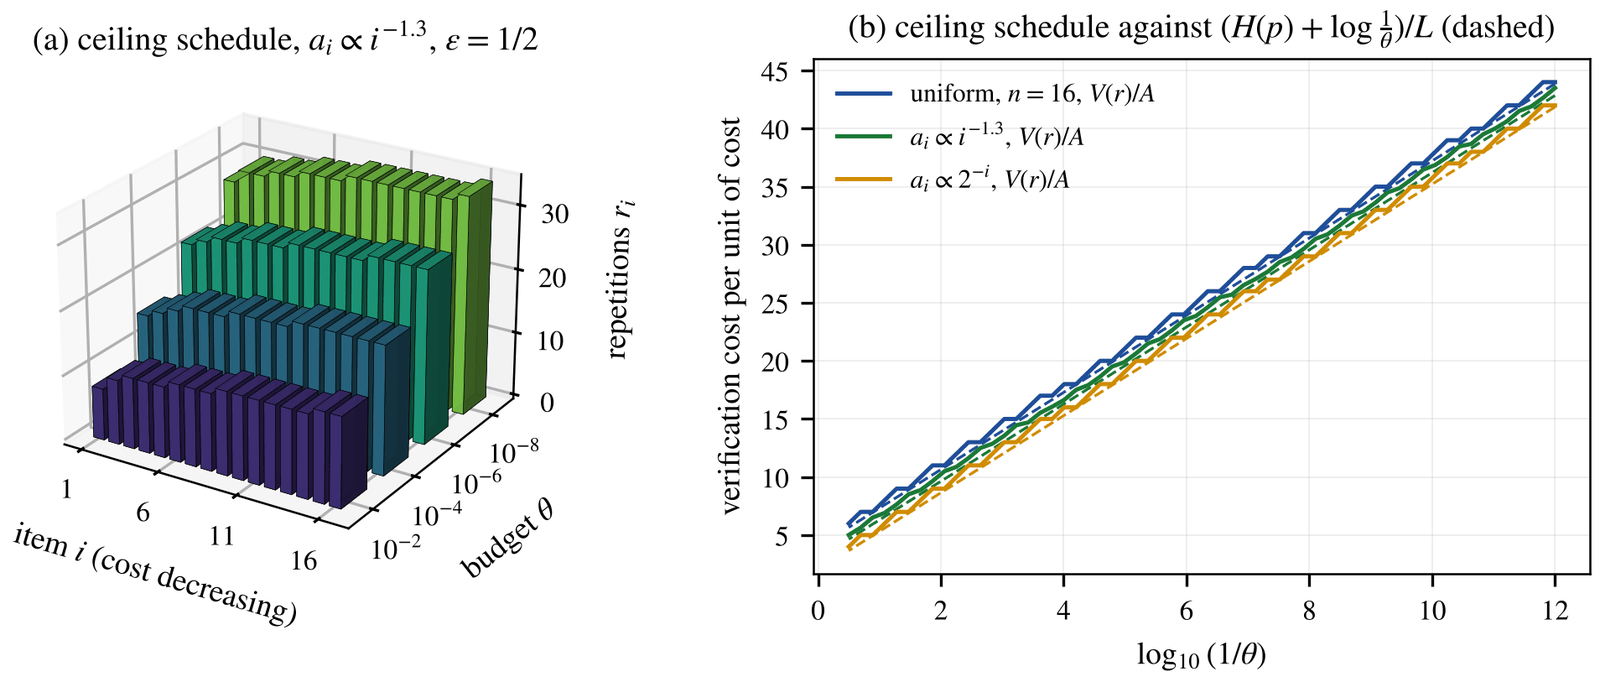
\includegraphics[width=0.98\textwidth]{figures/fig_schedule3d}
\caption{The entropy law. (a) The ceiling schedule $r_{i}=\lceil\log_{2}(A/(\theta a_{i}))\rceil$ for sixteen candidates with costs $a_{i}\propto i^{-1.3}$ and $\eps=\frac12$, at the budgets $\theta=10^{-2}$, $10^{-4}$, $10^{-6}$, $10^{-8}$: the expensive candidates receive the fewest runs, and each factor $100$ of $\theta$ adds six or seven runs to every check. (b) The cost of the ceiling schedule divided by $A$, for the uniform profile on sixteen candidates and the profiles $a_{i}\propto i^{-1.3}$ and $a_{i}\propto2^{-i}$ on sixteen, against the lower bound $(H(p)+\log\frac1\theta)/L$ (dashed). The curves stay in the band of width one above the bound, as Theorem~\ref{thm:A} asserts, and the more skewed the profile the lower the line.}
\label{fig:schedule}
\end{figure*}

\begin{corollary}[Equal costs]\label{cor:uniform}
For $n$ candidates of cost $a$ each, $\frac{na}{L}\log\frac n\theta\le\Vs(\theta)\le\frac{na}{L}\log\frac n\theta+na$. In particular the number of runs per candidate in an optimal schedule is $\log(n/\theta)/L+O(1)$.
\end{corollary}

\begin{proof}
Here $A=na$ and $H(p)=\log n$.
\end{proof}

\begin{proposition}[Shape of the optimum]\label{prop:shape}
Every optimal schedule is antitone in the costs: if $a_{i}>a_{j}$ then $r_{i}\le r_{j}$. The real relaxation, the minimum of $\sum a_{i}x_{i}$ over $x\in[0,\infty)^{n}$ with $\sum\eps^{x_{i}}\le\theta$, is attained only at $x_{i}=\log(A/(\theta a_{i}))/L$ and equals the lower bound of \eqref{eq:entropylaw}.
\end{proposition}

\begin{proof}
If $a_{i}>a_{j}$ and $r_{i}>r_{j}$, exchanging $r_{i}$ and $r_{j}$ keeps $\sum\eps^{r}$ and lowers the cost by $(a_{i}-a_{j})(r_{i}-r_{j})>0$, so $r$ was not optimal. For the relaxation, Proposition~\ref{prop:entropyineq} with $\beta_{i}=\eps^{x_{i}}$ gives $\sum a_{i}x_{i}\ge(A/L)(H+\log\frac1\theta)$, with equality exactly when $\eps^{x_{i}}=\theta p_{i}$.
\end{proof}

The marginal price of soundness is constant: lowering $\theta$ by a factor $e$ raises the lower bound by $A/L$, one nat of soundness bought on every check.

\begin{corollary}[Checks of different soundness]\label{cor:hetero}
If the check of candidate $i$ has soundness $\eps_{i}$, put $L_{i}=\log(1/\eps_{i})$, $b_{i}=a_{i}/L_{i}$, $B=\sum b_{i}$ and $q=b/B$. Then the least cost of a schedule with $\sum\eps_{i}^{r_{i}}\le\theta$, for $0<\theta\le1$, lies between $B(H(q)+\log\frac1\theta)$ and $B(H(q)+\log\frac1\theta)+A$.
\end{corollary}

\begin{proof}
The cost is $\sum a_{i}r_{i}=\sum b_{i}(r_{i}L_{i})$ and $\eps_{i}^{r_{i}}=e^{-r_{i}L_{i}}$. Proposition~\ref{prop:entropyineq} with weights $b_{i}$ and $\beta_{i}=e^{-r_{i}L_{i}}$ gives the lower bound, and $r_{i}=\lceil\log(B/(\theta b_{i}))/L_{i}\rceil$ gives $\sum\eps_{i}^{r_{i}}\le\theta\sum b_{i}/B=\theta$ and cost below $\sum b_{i}\log(B/(\theta b_{i}))+\sum a_{i}$.
\end{proof}

So the right unit of cost is the cost of one nat of soundness, $a_{i}/L_{i}$, and the entropy is that of the profile measured in this unit.

\subsection{Infinitely many candidates}

\begin{proposition}\label{prop:infinite}
Let $(a_{n})_{n\ge1}$ be positive with $A=\sum a_{n}<\infty$, and let $\Vs(\theta)$ be the infimum of $\sum a_{n}r_{n}$ over $r\in\NN^{\NN}$ with $\sum\eps^{r_{n}}\le\theta$. Then \eqref{eq:entropylaw} holds for $0<\theta\le1$, with both sides infinite when $H(p)=\infty$.
\end{proposition}

\begin{proof}
Let $r$ be feasible and $N\ge1$. The first $N$ terms satisfy $\sum_{n\le N}\eps^{r_{n}}\le\theta$, so the finite lower bound gives, with $A_{N}=\sum_{n\le N}a_{n}$ and by \eqref{eq:AH},
\[
\sum_{n\le N}a_{n}\log\frac1{a_{n}}+A_{N}\log A_{N}+A_{N}\log\frac1\theta\le L\sum_{n\le N}a_{n}r_{n}\le L\,V(r).
\]
The terms $a_{n}\log(1/a_{n})$ are positive once $a_{n}<1$, which holds for all large $n$, so as $N\to\infty$ the left side tends to $\sum_{n}a_{n}\log(1/a_{n})+A\log A+A\log(1/\theta)=A(H(p)+\log\frac1\theta)$, finite or infinite. This is the lower bound. The ceiling schedule $r_{n}=\lceil\log(A/(\theta a_{n}))/L\rceil$ satisfies $\sum\eps^{r_{n}}\le\theta\sum p_{n}=\theta$ and $V(r)\le(A/L)(H(p)+\log\frac1\theta)+A$ term by term.
\end{proof}

\subsection{Clean runs}

A stronger requirement than $\EE F\le\theta$ is that the whole run be clean with probability at least $1-\theta$: $\PR_{w}(F=0)\ge1-\theta$ in every world.

\begin{proposition}[Clean runs]\label{prop:clean}
Let $q_{i}=\eps^{r_{i}}$ and $0<\theta<1$. If $\sum q_{i}\le\theta$ then every world has $\PR_{w}(F=0)\ge1-\theta$. If the checks are sharp and every world has $\PR_{w}(F=0)\ge1-\theta$, then $\sum q_{i}\le\log\frac1{1-\theta}\le\frac{\theta}{1-\theta}$. Hence the least cost of a clean schedule lies between $\Vs(\log\frac1{1-\theta})$ and $\Vs(\theta)$, and Theorem~\ref{thm:A} holds for it with $\log\frac1\theta$ in the lower bound replaced by $\log\frac1\theta-\log\frac1{1-\theta}$.
\end{proposition}

\begin{proof}
In world $w$ the candidates are decided independently, so $\PR_{w}(F=0)=\prod_{i\text{ incorrect}}(1-q_{i}')$ with $q_{i}'\le q_{i}$, and this is at least $\prod_{i}(1-q_{i})$. By induction on $n$, $\prod_{i}(1-q_{i})\ge1-\sum_{i}q_{i}$ for $q_{i}\in[0,1]$: the step is $(1-s)(1-q)=1-s-q+sq\ge1-s-q$. This proves the first claim. In the world in which every candidate is incorrect, sharpness gives $1-\theta\le\prod_{i}(1-q_{i})\le\prod_{i}e^{-q_{i}}=e^{-\sum q_{i}}$, so $\sum q_{i}\le\log\frac1{1-\theta}$, and $\log\frac1{1-\theta}=\sum_{k\ge1}\theta^{k}/k\le\theta/(1-\theta)$.
\end{proof}

\subsection{Random schedules}

A schedule may be drawn at random, provided the draw is independent of the checks: the system may toss coins to decide how hard to test, but not look at the results to decide.

\begin{proposition}[Random oblivious schedules]\label{prop:random}
Let $R$ be a random schedule taking finitely many values $r^{(1)},\dots,r^{(m)}$ with probabilities $w_{1},\dots,w_{m}$, independent of the checks, with $\EE\sum_{i}\eps^{R_{i}}\le\theta$. Then $\EE\,V(R)\ge(A/L)(H(p)+\log\frac1\theta)$.
\end{proposition}

\begin{proof}
Let $\bar r=\sum_{j}w_{j}r^{(j)}\in[0,\infty)^{n}$. By the weighted inequality of arithmetic and geometric means, which is Jensen's inequality for the exponential \cite{Jen06}, $\eps^{\bar r_{i}}=\prod_{j}(\eps^{r^{(j)}_{i}})^{w_{j}}\le\sum_{j}w_{j}\eps^{r^{(j)}_{i}}$, so $\sum_{i}\eps^{\bar r_{i}}\le\EE\sum_{i}\eps^{R_{i}}\le\theta$. Proposition~\ref{prop:entropyineq} with $\beta_{i}=\eps^{\bar r_{i}}$ gives $L\sum_{i}a_{i}\bar r_{i}\ge A(H+\log\frac1\theta)$, and $\sum a_{i}\bar r_{i}=\EE\,V(R)$.
\end{proof}

\begin{remark}[Adaptive protocols]\label{rem:adaptive}
The hypothesis that the schedule ignores the outcomes cannot be dropped. Consider the protocol that gives every check $r=\lceil\log(1/\theta)/L\rceil$ runs and halts the whole process, rejecting every later candidate, at the first rejection. In a world with incorrect candidates $i_{1}<i_{2}<\cdots$, the $j$-th of them is kept only if it and the $j-1$ before it are all falsely accepted, which has probability at most $\theta^{j}$, so $\EE_{w}F\le\sum_{j\ge1}\theta^{j}=\theta/(1-\theta)$. Its cost in the world in which every candidate is correct is $Ar<(A/L)\log\frac1\theta+A$, without the entropy term. The saving is paid for elsewhere: a single incorrect candidate stops the process and every correct candidate after it is lost. Theorem~\ref{thm:A} is therefore a theorem about protocols that decide each candidate on its own evidence, which is what a system that must keep its correct work has to do; whether an entropy term returns for adaptive protocols that keep every correct candidate and are charged their worst-case cost is a question we leave open.
\end{remark}

\subsection{Two-sided checks}\label{ssec:twosided}

Learned verifiers err in both directions. Suppose a run of the check of candidate $i$ returns the correct verdict with probability $1-q$ and the wrong one with probability $q<\frac12$, for correct and incorrect candidates alike, and the protocol keeps the candidate when a majority of $r_{i}$ runs, $r_{i}$ odd, accept. Then there are false acceptances and false rejections, and we ask that the expected number of each be at most $\theta$. Write
\[
D=\tfrac12\log\frac1{4q(1-q)}=\mathrm{KL}\bigl(\mathrm{Ber}(\tfrac12)\,\big\|\,\mathrm{Ber}(q)\bigr),
\]
the Chernoff exponent of the majority test \cite{Che52,CT06}.

\begin{proposition}[Two-sided checks]\label{prop:twosided}
\begin{enumerate}[label=\textup{(\roman*)},leftmargin=2.2em,itemsep=1pt]
\item A majority of $r$ runs errs with probability at most $(4q(1-q))^{r/2}=e^{-Dr}$.
\item For $0<\theta\le1$ the schedule $r_{i}$ equal to the least odd integer at least $\log(A/(\theta a_{i}))/D$ has at most $\theta$ expected false acceptances and at most $\theta$ expected false rejections, and costs at most $(A/D)(H(p)+\log\frac1\theta)+2A$.
\item Every decision rule that keeps a candidate whose runs all accept, used with any schedule with at most $\theta$ expected false acceptances in every world, costs at least $(A/\log(1/q))(H(p)+\log\frac1\theta)$.
\end{enumerate}
\end{proposition}

\begin{proof}
(i) Let $S$ be the number of wrong verdicts among $r$ runs, a binomial variable with parameters $r$ and $q$; the majority errs when $S\ge r/2$. For $t>0$, Markov's inequality applied to $e^{tS}$ gives $\PR(S\ge r/2)\le e^{-tr/2}(1-q+qe^{t})^{r}$. With $e^{t}=(1-q)/q>1$ the bracket is $2(1-q)$ and $e^{-tr/2}=(q/(1-q))^{r/2}$, so the bound is $2^{r}(1-q)^{r/2}q^{r/2}=(4q(1-q))^{r/2}$.
(ii) By (i) each candidate is misjudged with probability at most $e^{-Dr_{i}}\le\theta a_{i}/A$, whichever its label, so the expected numbers of both errors are at most $\theta$; and $r_{i}<\log(A/(\theta a_{i}))/D+2$.
(iii) An incorrect candidate whose $r_{i}$ runs all return the wrong verdict is kept, which has probability $q^{r_{i}}$; in the world in which every candidate is incorrect the expected number of false acceptances is at least $\sum q^{r_{i}}$, so $\sum q^{r_{i}}\le\theta$, and Proposition~\ref{prop:entropyineq} with $\beta_{i}=q^{r_{i}}$ gives the bound.
\end{proof}

The rate $D$ is the exact exponent of the majority vote: by the method of types, $\PR(S\ge r/2)\ge(r+1)^{-1}e^{-r\,\mathrm{KL}(\lceil r/2\rceil/r\,\|\,q)}$ \cite{CT06}, and $\mathrm{KL}(\lceil r/2\rceil/r\,\|\,q)\to D$. So for two-sided checks the entropy law holds with $L$ replaced by $D$, and the price of a check that can err in both directions, compared with a one-sided check of the same per-run error $q$, is the ratio $\log(1/q)/D$, which tends to $2$ as $q\to0$ and to infinity as $q\to\frac12$.

\section{Huffman schedules}\label{sec:huffman}

When the soundness of a run is the reciprocal of an integer and the budget is a power of it, the optimal schedule is not only close to the entropy bound but computable exactly, and it is a code.

\subsection{Schedules are codes}

A $D$-ary \emph{prefix code} for $n$ symbols is a set of $n$ words over an alphabet of $D$ letters, none a prefix of another. Kraft's inequality says that lengths $\ell_{1},\dots,\ell_{n}\in\NN$ are the lengths of a prefix code if and only if $\sum_{i}D^{-\ell_{i}}\le1$ \cite{Kra49}, and McMillan's theorem extends the necessity to all uniquely decodable codes \cite{McM56}; Appendix~\ref{app:kraft} recalls the proofs. For a probability vector $p$ write $L_{D}(p)$ for the least value of $\sum_{i}p_{i}\ell_{i}$ over lengths satisfying Kraft's inequality, and $H_{D}(p)=H(p)/\log D$.

\begin{lemma}[Kraft form of soundness]\label{lem:kraftsound}
Let $D>1$ and $k\in\NN$, and let $r\in\NN^{n}$.
\begin{enumerate}[label=\textup{(\roman*)},leftmargin=2.2em,itemsep=1pt]
\item If $\sum_{i}D^{-r_{i}}\le D^{-k}$, then $r_{i}\ge k$ for every $i$ and $\ell_{i}=r_{i}-k$ satisfies $\sum_{i}D^{-\ell_{i}}\le1$.
\item If $\sum_{i}D^{-\ell_{i}}\le1$, then $r_{i}=\ell_{i}+k$ satisfies $\sum_{i}D^{-r_{i}}\le D^{-k}$.
\item $\sum_{i}a_{i}(\ell_{i}+k)=kA+\sum_{i}a_{i}\ell_{i}$.
\end{enumerate}
\end{lemma}

\begin{proof}
(i) Each term satisfies $D^{-r_{i}}\le\sum_{j}D^{-r_{j}}\le D^{-k}$, and $x\mapsto D^{-x}$ is decreasing, so $r_{i}\ge k$; then $\sum D^{-(r_{i}-k)}=D^{k}\sum D^{-r_{i}}\le1$. (ii) $\sum D^{-(\ell_{i}+k)}=D^{-k}\sum D^{-\ell_{i}}\le D^{-k}$. (iii) is linearity.
\end{proof}

\begin{proof}[Proof of Theorem~\ref{thm:C}]
With $\eps=1/D$ and $\theta=D^{-k}$, the $\theta$-sound schedules are the $r$ with $\sum D^{-r_{i}}\le D^{-k}$. By Lemma~\ref{lem:kraftsound} they are exactly the vectors $\ell+k$ with $\ell$ satisfying Kraft's inequality, which by Kraft's theorem are the length vectors of prefix codes. The cost is $kA+\sum a_{i}\ell_{i}=A(k+\sum p_{i}\ell_{i})$, and its minimum is $A(k+L_{D}(p))$. Huffman's algorithm produces a prefix code of expected length $L_{D}(p)$ (Appendix~\ref{app:huffman}).
\end{proof}

So the optimal schedule is obtained by building the Huffman tree of the cost profile and adding $k$ runs to every check (Fig.~\ref{fig:kraft}). Each run of a check is a letter of the codeword of its candidate; the first $k$ letters buy the budget $D^{-k}$, the remaining $\ell_{i}$ letters distinguish the candidate from the others, and a candidate of high cost gets a short word, as a frequent symbol does.

\begin{figure*}[t]
\centering
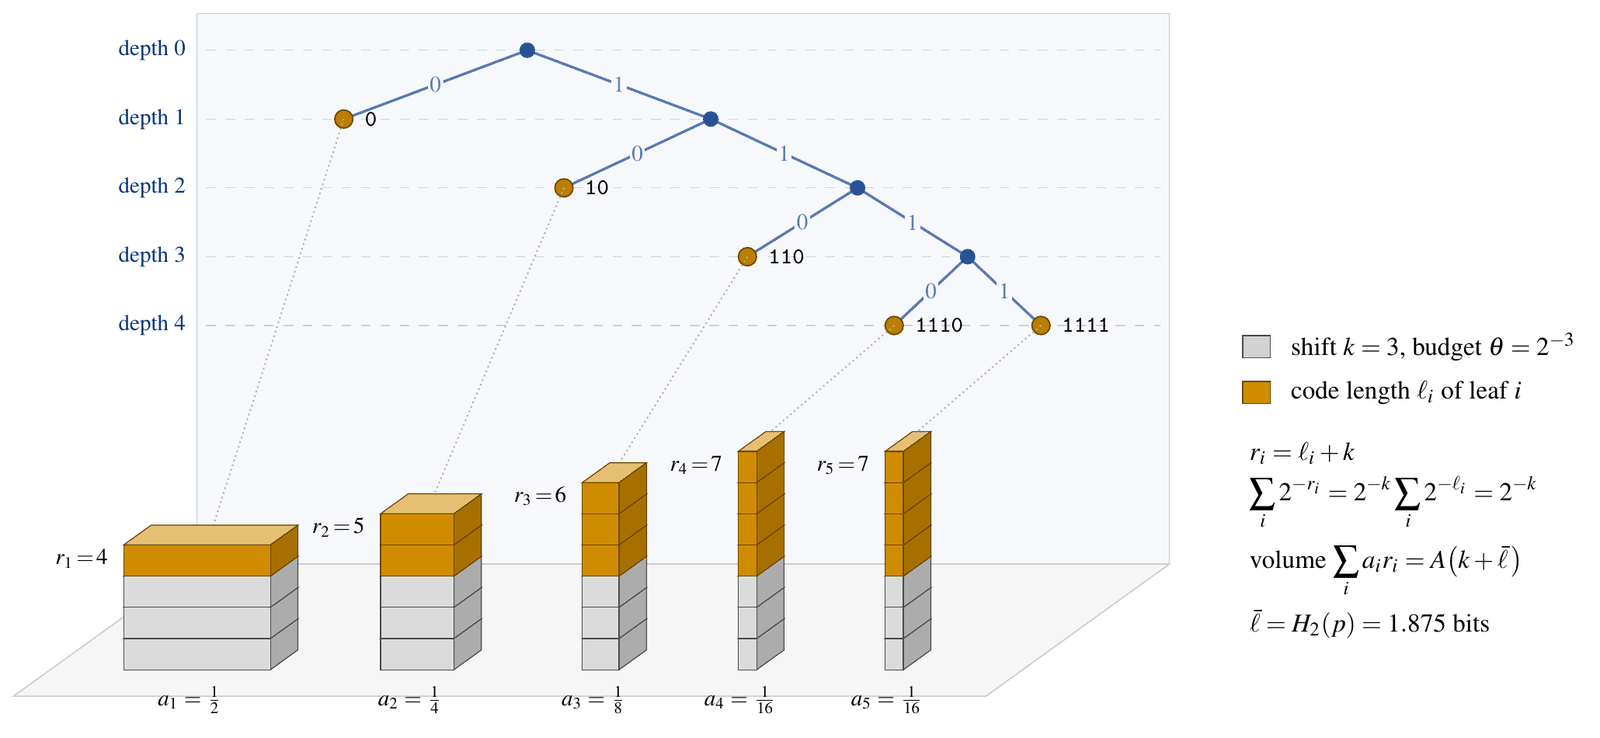
\includegraphics[width=0.92\textwidth]{figures/fig_kraft3d}
\caption{Theorem~\ref{thm:C} for the profile $p=(\frac12,\frac14,\frac18,\frac1{16},\frac1{16})$, $\eps=\frac12$ and $\theta=2^{-3}$. Back wall: the binary Huffman tree, with codewords $0$, $10$, $110$, $1110$, $1111$. Floor: a column for each candidate, of width proportional to its cost $a_{i}$, built from $k=3$ grey blocks, which buy the budget $2^{-3}$, and $\ell_{i}$ gold blocks, one per letter of its codeword. The heights are the optimal numbers of runs $r_{i}=4,5,6,7,7$, the budget is exactly spent, $\sum2^{-r_{i}}=2^{-3}$, and the volume of the columns is the optimal cost $A(k+\bar\ell)$ with $\bar\ell=H_{2}(p)=1.875$.}
\label{fig:kraft}
\end{figure*}

\begin{corollary}\label{cor:huffbounds}
Under the hypotheses of Theorem~\ref{thm:C}, $A(k+H_{D}(p))\le\Vs(D^{-k})<A(k+H_{D}(p)+1)$, with equality on the left if and only if every $p_{i}$ is an integer power of $1/D$.
\end{corollary}

\begin{proof}
Shannon's bounds $H_{D}(p)\le L_{D}(p)<H_{D}(p)+1$ \cite{Sha48,CT06} are the case $\theta=1$ of Theorem~\ref{thm:A}, since $L=\log D$ and $(A/L)H(p)=AH_{D}(p)$; the equality case is that of Proposition~\ref{prop:entropyineq}.
\end{proof}

The strict inequality on the right is slightly better than Theorem~\ref{thm:A}, and Gallager's bound improves it further when the largest cost share is small \cite{Gal78}: the redundancy $L_{2}(p)-H_{2}(p)$ is at most $p_{\max}+0.086$ when the largest share $p_{\max}$ is below one half. So the additive constant $A$ of the entropy law is, in this case, the redundancy of an optimal code.

\subsection{Examples}

Table~\ref{tab:huffman} compares three schedules on two profiles: the Huffman schedule, the ceiling schedule of Theorem~\ref{thm:A}, and the lower bound. On a dyadic profile the three agree. On a profile that is not dyadic the ceiling schedule overspends, because the Shannon lengths $\lceil\log_{2}(1/p_{i})\rceil$ are not optimal, and the Huffman schedule lies between it and the bound.

\begin{table}[b]
\caption{Schedules for $\eps=\frac12$, $\theta=2^{-3}$. Costs are $V/A$.}
\label{tab:huffman}
\centering
\small
\begin{tabular}{@{}l l l@{}}
\toprule
 & $p=(\frac12,\frac14,\frac18,\frac1{16},\frac1{16})$ & $p=(0.4,0.3,0.2,0.1)$ \\
\midrule
Huffman lengths $\ell$ & $(1,2,3,4,4)$ & $(1,2,3,3)$ \\
Huffman schedule $r$ & $(4,5,6,7,7)$ & $(4,5,6,6)$ \\
$\sum2^{-r_{i}}$ & $2^{-3}$ & $2^{-3}$ \\
cost, Huffman & $4.875$ & $4.900$ \\
ceiling schedule $r$ & $(4,5,6,7,7)$ & $(5,5,6,7)$ \\
cost, ceiling & $4.875$ & $5.400$ \\
bound $3+H_{2}(p)$ & $4.875$ & $4.846$ \\
\bottomrule
\end{tabular}
\end{table}

Figure~\ref{fig:huffman} runs the comparison over twelve profiles: uniform, Zipf, geometric and random. The Huffman cost minus $k$ is the Huffman length, which lies in $[H_{2}(p),H_{2}(p)+1)$ and equals $H_{2}(p)$ only for the dyadic profiles.

\begin{figure*}[t]
\centering
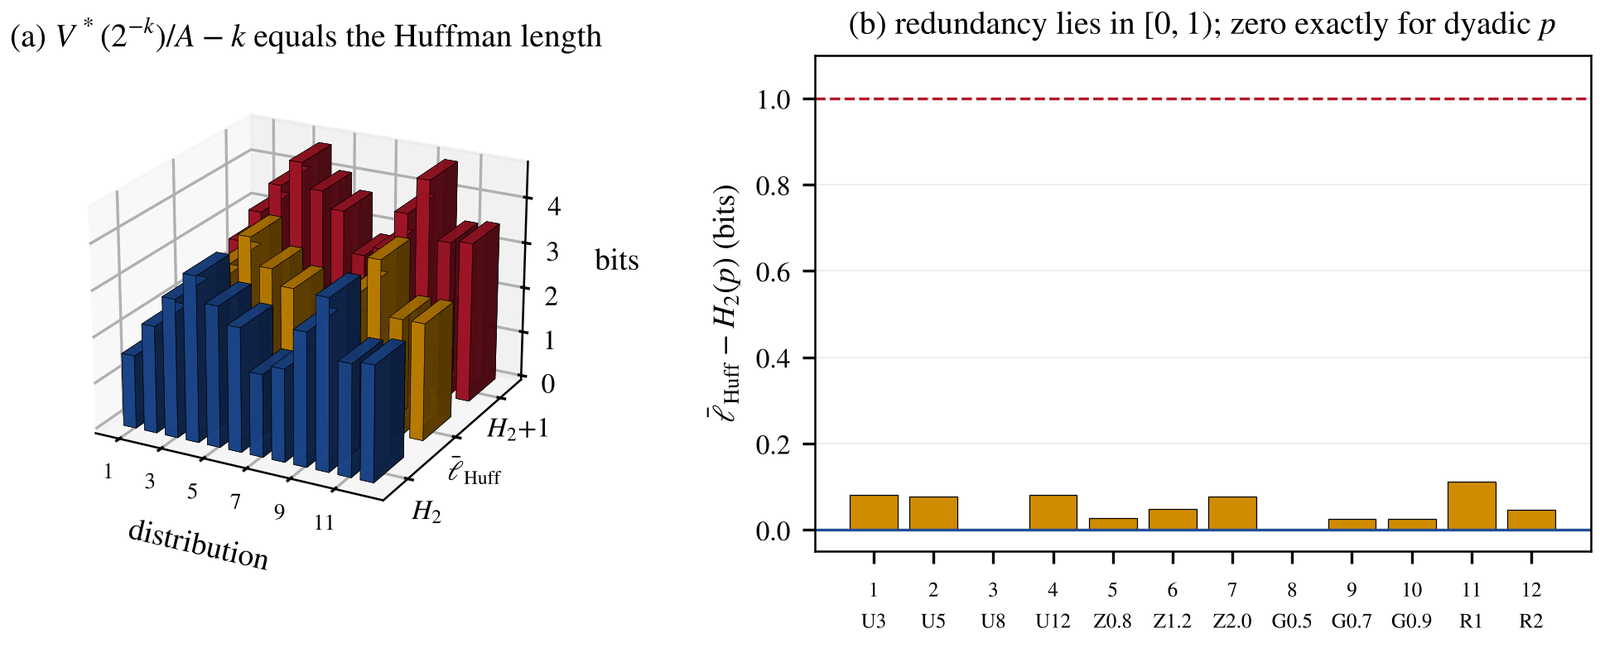
\includegraphics[width=0.98\textwidth]{figures/fig_huffman3d}
\caption{Theorem~\ref{thm:C} on twelve profiles: uniform on $3$, $5$, $8$ and $12$ candidates (U), Zipf with exponents $0.8$, $1.2$ and $2$ on ten (Z), geometric with ratios $0.5$, $0.7$ and $0.9$ on fourteen (G), and two random profiles on nine (R). (a) For each profile, the entropy $H_{2}(p)$, the optimal schedule cost $\Vs(2^{-k})/A-k$, which is the Huffman length, and $H_{2}(p)+1$. (b) The redundancy $\Vs/A-k-H_{2}(p)$, which lies in $[0,1)$; it vanishes on the dyadic profile, the uniform one on eight candidates (green), and is $2.7\times10^{-5}$ for the geometric profile of ratio one half, whose normalised weights differ from powers of two by the factor $2/(2-2^{-13})$. The largest redundancy, $0.112$, is that of the first random profile.}
\label{fig:huffman}
\end{figure*}

\begin{remark}[Larger alphabets]
For $D\ge3$ Huffman's algorithm merges the $D$ smallest weights at each step, after adding zero weights until $n\equiv1\pmod{D-1}$; the dummy candidates receive the longest codewords and cost nothing (Appendix~\ref{app:huffman}). A check of soundness $1/3$ run $r$ times is a ternary codeword of length $r$.
\end{remark}

\section{The R\'enyi law and the duality criterion}\label{sec:renyi}

\subsection{Polynomial checks}

A check is \emph{exponential} when $r$ runs drive its false acceptance probability to $\eps^{r}$, so that the cost of reaching $\delta$ is $a\log(1/\delta)/L$. Many checks are slower. A statistical check that averages $m$ independent samples of a statistic and accepts when the average is close to its target is the basic example.

\begin{example}[Chebyshev checks]\label{ex:chebyshev}
Let a candidate determine a random variable $X$ with variance at most $\sigma^{2}$, with mean $0$ if the candidate is correct and mean at least $2t>0$ if it is incorrect, and let the check accept when the mean of $m$ independent samples is below $t$. By Chebyshev's inequality an incorrect candidate is accepted, and a correct one rejected, with probability at most $\sigma^{2}/(mt^{2})$. So false acceptance probability $\delta$ costs $m=\sigma^{2}/(t^{2}\delta)$ samples: the cost is $a\,\delta^{-1}$ with $a$ proportional to $\sigma^{2}/t^{2}$.
\end{example}

We say a family of checks has \emph{polynomial order} $s>0$ if the check of candidate $i$ reaches false acceptance probability $\delta_{i}\in(0,1]$ at cost $a_{i}\delta_{i}^{-s}$, and that an allocation $\delta$ is $\theta$-sound if $\sum_{i}\delta_{i}\le\theta$. Chebyshev checks have order $1$. Let $\Vs_{s}(\theta)$ be the infimum of $\sum_{i}a_{i}\delta_{i}^{-s}$ over $\theta$-sound allocations. For $0<\alpha<1$ the R\'enyi entropy of order $\alpha$ is
\[
H_{\alpha}(p)=\frac1{1-\alpha}\log\sum_{i}p_{i}^{\alpha},
\]
which decreases from $\log n$ at $\alpha\to0$ to $H(p)$ at $\alpha\to1$ \cite{Ren61,CT06}.

\begin{proof}[Proof of Theorem~\ref{thm:D}]
\emph{Lower bound.} Put $\alpha=1/(1+s)$, so that $1/\alpha=1+s$ and $1/(1-\alpha)=(1+s)/s$ are conjugate exponents. Write $a_{i}^{\alpha}=(a_{i}\delta_{i}^{-s})^{\alpha}\,\delta_{i}^{s\alpha}$ and apply H\"older's inequality:
\[
\begin{aligned}
\sum_{i}a_{i}^{\alpha}&\le\Bigl(\sum_{i}a_{i}\delta_{i}^{-s}\Bigr)^{\alpha}\Bigl(\sum_{i}\delta_{i}^{s\alpha/(1-\alpha)}\Bigr)^{1-\alpha}\\
&=\Bigl(\sum_{i}a_{i}\delta_{i}^{-s}\Bigr)^{\frac1{1+s}}\Bigl(\sum_{i}\delta_{i}\Bigr)^{\frac s{1+s}},
\end{aligned}
\]
since $s\alpha/(1-\alpha)=1$. With $\sum\delta_{i}\le\theta$ and raising to the power $1+s$, $(\sum_{i}a_{i}^{\alpha})^{1+s}\le\theta^{s}\sum_{i}a_{i}\delta_{i}^{-s}$.

\emph{Attainment.} Let $S=\sum_{j}a_{j}^{\alpha}$ and $\delta_{i}=\theta a_{i}^{\alpha}/S$. Then $\sum\delta_{i}=\theta$, $\delta_{i}\le\theta\le1$ because $a_{i}^{\alpha}\le S$, and $\sum_{i}a_{i}\delta_{i}^{-s}=\theta^{-s}S^{s}\sum_{i}a_{i}^{1-s\alpha}=\theta^{-s}S^{s}\sum_{i}a_{i}^{\alpha}=\theta^{-s}S^{1+s}$, because $1-s\alpha=\alpha$.

\emph{Entropy form.} $S=A^{\alpha}\sum_{i}p_{i}^{\alpha}$, so $S^{1+s}=A\,(\sum_{i}p_{i}^{\alpha})^{1+s}$, and $(1+s)\log\sum p_{i}^{\alpha}=\frac{1+s}{s}\,s\log\sum p_{i}^{\alpha}=s\,H_{\alpha}(p)$, since $1-\alpha=s/(1+s)$.

\emph{The limit $s\to0$.} For finitely many candidates $\alpha\mapsto\log\sum p_{i}^{\alpha}$ is smooth and vanishes at $\alpha=1$ with derivative $\sum p_{i}\log p_{i}=-H(p)$ there, so $H_{\alpha}(p)=H(p)+O(1-\alpha)=H(p)+O(s)$. Hence $\Vs_{s}(\theta)/A=\exp\bigl(s(H_{\alpha}(p)+\log\frac1\theta)\bigr)=1+s\bigl(H(p)+\log\frac1\theta\bigr)+O(s^{2})$.
\end{proof}

The optimal allocation gives the $i$-th check the share $a_{i}^{\alpha}/S$ of the budget, a flattened version of the share $a_{i}/A$ of the exponential case: when checks are slow, expensive checks must still be made quite reliable, because buying reliability anywhere is costly. The two laws are related by a limit. Since $\frac1L\log\frac1\delta=\lim_{s\to0}\frac{\delta^{-s}-1}{sL}$, the cost of an exponential check is the derivative at $s=0$ of the cost of a polynomial one, and
\[
\lim_{s\to0}\frac{\Vs_{s}(\theta)-A}{sL}=\frac AL\Bigl(H(p)+\log\frac1\theta\Bigr),
\]
which is the real relaxation of the entropy law (Proposition~\ref{prop:shape}). Campbell's coding theorem has the same structure, with exponentially weighted codeword lengths and the R\'enyi entropy of order $1/(1+t)$ \cite{Cam65}.

\begin{corollary}[Equal costs]\label{cor:polyuniform}
For $n$ candidates of cost $a$ and checks of order $s$, $\Vs_{s}(\theta)=a\,n^{1+s}\theta^{-s}$. Chebyshev checks cost $an^{2}/\theta$, against $(an/L)\log(n/\theta)+O(an)$ for exponential checks.
\end{corollary}

So the tax per candidate is $(n/\theta)^{s}$ for polynomial checks and $\log(n/\theta)/L$ for exponential ones: a statistical check that is not amplified exponentially makes the certification of a long run of modifications quadratically expensive. Figure~\ref{fig:renyi} shows the law and its tangent at $s=0$.

\begin{figure*}[t]
\centering
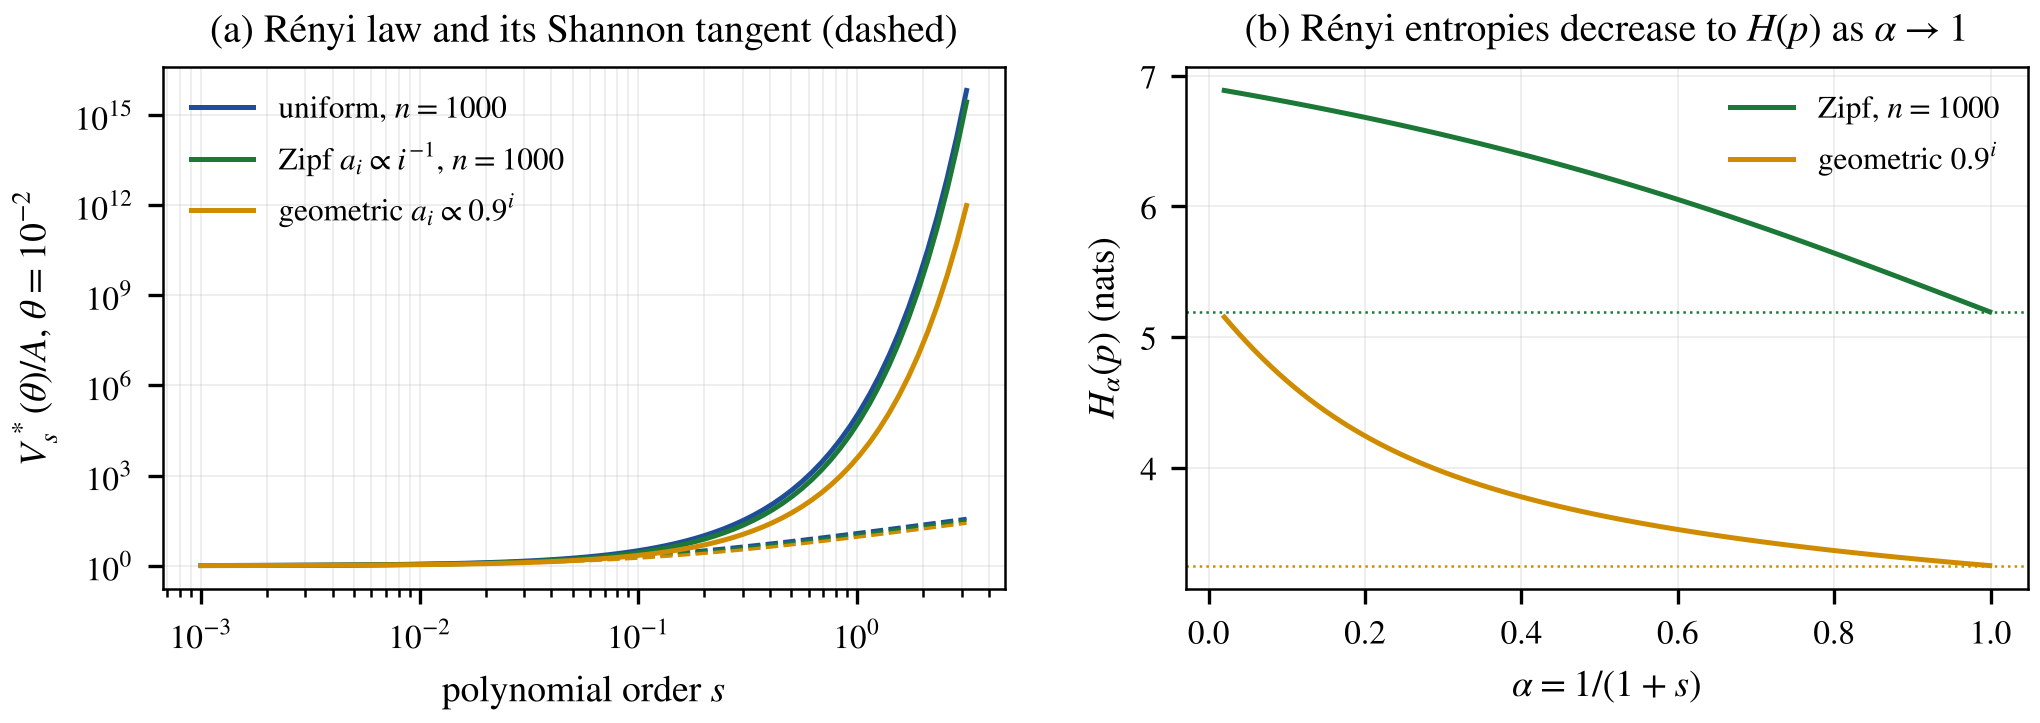
\includegraphics[width=0.98\textwidth]{figures/fig_renyi}
\caption{The R\'enyi law, Theorem~\ref{thm:D}. (a) $\Vs_{s}(\theta)/A=\theta^{-s}e^{sH_{1/(1+s)}(p)}$ at $\theta=10^{-2}$ for a uniform profile and a Zipf profile on a thousand candidates and a geometric profile of ratio $0.9$, with the Shannon tangents $1+s(H(p)+\log\frac1\theta)$ (dashed). The tangents are exact as $s\to0$ and the flat profile is the most expensive at every order. (b) The R\'enyi entropies $H_{\alpha}(p)$ of the Zipf and geometric profiles as functions of $\alpha=1/(1+s)$, decreasing to the Shannon entropy (dotted) as $\alpha\to1$.}
\label{fig:renyi}
\end{figure*}

\subsection{The duality criterion}

For infinitely many candidates the question is not the value of the optimum but whether a sound allocation of finite cost exists. The answer, for every cost function, is a single series.

Let $\kappa\colon(0,1]\to[0,\infty)$ be the cost, per unit of $a$, of making a check accept an incorrect candidate with probability at most $\delta$; so $\kappa(\delta)=\log(1/\delta)/L$ for exponential checks with a real number of runs and $\kappa(\delta)=\delta^{-s}$ for checks of order $s$. Define the \emph{dual cost}
\[
\psi(u)=\inf_{0<\delta\le1}\bigl(\kappa(\delta)+u\delta\bigr),\qquad u\ge0,
\]
the least cost of a check when each unit of false acceptance probability is charged $u$. It is the concave conjugate of $\kappa$ restricted to $(0,1]$.

\begin{theorem}[Duality criterion]\label{thm:dual}
Let $a_{n}>0$. The following are equivalent.
\begin{enumerate}[label=\textup{(\alph*)},leftmargin=2.2em,itemsep=1pt]
\item There are $\delta_{n}\in(0,1]$ with $\sum_{n}\delta_{n}<\infty$ and $\sum_{n}a_{n}\kappa(\delta_{n})<\infty$.
\item $\sum_{n}a_{n}\psi(\lambda/a_{n})<\infty$ for some $\lambda>0$.
\item $\sum_{n}a_{n}\psi(\lambda/a_{n})<\infty$ for every $\lambda>0$.
\end{enumerate}
When they hold, for every $\theta>0$ there are $\delta_{n}\in(0,1]$ with $\sum\delta_{n}\le\theta$ and $\sum a_{n}\kappa(\delta_{n})<\infty$.
\end{theorem}

\begin{proof}
(a)$\Rightarrow$(c). For every $\lambda>0$ and $n$, $0\le a_{n}\psi(\lambda/a_{n})\le a_{n}\kappa(\delta_{n})+\lambda\delta_{n}$, and the right side is summable.
(c)$\Rightarrow$(b) is trivial.
(b)$\Rightarrow$(a). By the definition of the infimum choose $\delta_{n}\in(0,1]$ with $\kappa(\delta_{n})+(\lambda/a_{n})\delta_{n}\le\psi(\lambda/a_{n})+2^{-n}/a_{n}$. Then $a_{n}\kappa(\delta_{n})+\lambda\delta_{n}\le a_{n}\psi(\lambda/a_{n})+2^{-n}$, a summable bound for two nonnegative terms, so both $\sum a_{n}\kappa(\delta_{n})$ and $\sum\delta_{n}$ converge.
For the last claim choose $N$ with $\sum_{n>N}\delta_{n}\le\theta/2$ and replace $\delta_{n}$ by $\theta/(2N)$ for $n\le N$; this changes finitely many finite terms of the cost.
\end{proof}

\begin{proposition}[The two dual costs]\label{prop:dualcosts}
\begin{enumerate}[label=\textup{(\roman*)},leftmargin=2.2em,itemsep=1pt]
\item For exponential checks, $\kappa(\delta)=\log(1/\delta)/L$, the dual is
\[
\psi(u)=\begin{cases}(1+\log(uL))/L,&uL\ge1,\\ u,&uL<1.\end{cases}
\]
\item For checks of order $s$, $\kappa(\delta)=\delta^{-s}$, the dual is
\[
\psi(u)=\begin{cases}(1+s)\,s^{-s/(1+s)}u^{s/(1+s)},&u\ge s,\\ 1+u,&u<s.\end{cases}
\]
\end{enumerate}
\end{proposition}

\begin{proof}
Both functions $\delta\mapsto\kappa(\delta)+u\delta$ are convex on $(0,1]$. In (i) the derivative $-1/(L\delta)+u$ vanishes at $\delta=1/(uL)$, which lies in $(0,1]$ exactly when $uL\ge1$, with value $\log(uL)/L+1/L$; otherwise the derivative is negative on $(0,1]$ and the minimum is at $\delta=1$. In (ii) the derivative $-s\delta^{-s-1}+u$ vanishes at $\delta=(s/u)^{1/(1+s)}$, which lies in $(0,1]$ exactly when $u\ge s$, with value $(s/u)^{-s/(1+s)}+u(s/u)^{1/(1+s)}=(1+s)s^{-s/(1+s)}u^{s/(1+s)}$; otherwise the minimum is at $\delta=1$.
\end{proof}

\begin{corollary}\label{cor:dualcases}
Let $a_{n}\to0$.
\begin{enumerate}[label=\textup{(\roman*)},leftmargin=2.2em,itemsep=1pt]
\item Exponential checks with real numbers of runs admit a sound allocation of finite cost if and only if $\sum a_{n}<\infty$ and $\sum a_{n}\log(1/a_{n})<\infty$.
\item Checks of order $s$ admit one if and only if $\sum a_{n}^{1/(1+s)}<\infty$.
\end{enumerate}
\end{corollary}

\begin{proof}
For large $n$, $u=\lambda/a_{n}$ is large, and by Proposition~\ref{prop:dualcosts} $a_{n}\psi(\lambda/a_{n})$ equals $\frac{a_{n}}L\bigl(1+\log(\lambda L)+\log\frac1{a_{n}}\bigr)$ in case (i) and a constant multiple of $a_{n}^{1/(1+s)}$ in case (ii). In case (i) the sum converges if and only if $\sum a_{n}(1+\log\frac1{a_{n}})$ does, and both terms are eventually positive. Theorem~\ref{thm:dual} concludes.
\end{proof}

The integer version needs no duality.

\begin{proposition}[Integer schedules]\label{prop:integer}
Let $0<a_{n}\le1$ with $\sum a_{n}<\infty$. There is $r\in\NN^{\NN}$ with $\sum\eps^{r_{n}}<\infty$ and $\sum a_{n}r_{n}<\infty$ if and only if $\sum a_{n}\log(1/a_{n})<\infty$; the schedule $r_{n}=\lceil\log(1/a_{n})/L\rceil$ then works, and adding $k$ runs to every check multiplies $\sum\eps^{r_{n}}$ by $\eps^{k}$.
\end{proposition}

\begin{proof}
If $r$ is such a schedule, Lemma~\ref{lem:gibbs} with $x=a_{n}$ and $y=\eps^{r_{n}}$ gives $a_{n}\log(1/a_{n})\le a_{n}r_{n}L+\eps^{r_{n}}-a_{n}\le L\,a_{n}r_{n}+\eps^{r_{n}}$, a summable bound for a nonnegative sequence. Conversely $r_{n}=\lceil\log(1/a_{n})/L\rceil$ gives $\eps^{r_{n}}\le a_{n}$ and $a_{n}r_{n}\le a_{n}\log(1/a_{n})/L+a_{n}$. The last claim is $\eps^{r_{n}+k}=\eps^{k}\eps^{r_{n}}$.
\end{proof}

Theorem~\ref{thm:dual} is the infinite form of the entropy and R\'enyi laws: it says which cost profiles can be certified at all, and Section~\ref{sec:singularity} applies it to self-improving chains.

\section{Self-improvement chains}\label{sec:chains}

\subsection{The chain}

A BLLM improves itself in steps. At step $i$ the generator proposes candidates for the $i$-th modification until one is kept, then moves to step $i+1$. A candidate for step $i$ costs $g_{i}\ge0$ to generate, is incorrect with probability $\rho_{i}$, independently of everything else, and is checked by $r_{i}$ runs of a sharp check of soundness $\eps$ and cost $a_{i}$ per run, stopping at the first rejection. Let $T_{i}$ be the total cost of step $i$, $F$ the number of steps whose kept candidate is incorrect, $G=\sum g_{i}$, and write $\beta_{i}=\eps^{r_{i}}$.

\begin{lemma}[One step]\label{lem:onestep}
Let $s_{i}=1-\rho_{i}+\rho_{i}\beta_{i}$ be the probability that a candidate is kept and $\pi_{i}=\rho_{i}\beta_{i}/s_{i}$ the probability that the kept candidate is incorrect. Then
\[
g_{i}+a_{i}r_{i}\ \le\ \EE\,T_{i}\ \le\ \frac{g_{i}+a_{i}r_{i}}{1-\rho_{i}},\qquad \rho_{i}\beta_{i}\ \le\ \pi_{i}\ \le\ \frac{\rho_{i}\beta_{i}}{1-\rho_{i}} .
\]
\end{lemma}

\begin{proof}
The number of candidates proposed at step $i$ is geometric with success probability $s_{i}$, so its mean is $1/s_{i}$, and by Wald's identity $\EE\,T_{i}$ is $1/s_{i}$ times the expected cost $c_{i}$ of one candidate. A candidate costs $g_{i}$ plus at most $r_{i}$ runs, so $c_{i}\le g_{i}+a_{i}r_{i}$, and $s_{i}\ge1-\rho_{i}$; this is the upper bound. The kept candidate passed all its $r_{i}$ runs, so it alone costs $g_{i}+a_{i}r_{i}$; this is the lower bound. The bounds on $\pi_{i}$ follow from $1-\rho_{i}\le s_{i}\le1$.
\end{proof}

\begin{mainthm}[Chain law]\label{thm:B}
Let $0<\rho_{\ast}\le\rho_{i}\le\bar\rho<1$ for every $i$, and let $C^{*}(\theta)$ be the least value of $\sum_{i}\EE\,T_{i}$ over schedules with $\EE F\le\theta$. Then
\[
\begin{aligned}
C^{*}(\theta)&\ \ge\ G+\frac AL\Bigl(H(p)+\log\frac{\rho_{\ast}}{\theta}\Bigr),\\
C^{*}(\theta)&\ \le\ \frac1{1-\bar\rho}\Bigl[G+\frac AL\Bigl(H(p)+\log\frac{\bar\rho}{(1-\bar\rho)\theta}\Bigr)+A\Bigr],
\end{aligned}
\]
the upper bound for $0<\theta\le\bar\rho/(1-\bar\rho)$.
\end{mainthm}

\begin{proof}
$\EE F=\sum_{i}\pi_{i}$. If $\EE F\le\theta$, then $\rho_{\ast}\sum\beta_{i}\le\sum\pi_{i}\le\theta$ by Lemma~\ref{lem:onestep}, so $r$ is feasible for the budget $\theta/\rho_{\ast}$, and Proposition~\ref{prop:entropyineq} gives $V(r)\ge(A/L)(H+\log(\rho_{\ast}/\theta))$; also $\sum\EE\,T_{i}\ge G+V(r)$. Conversely let $\theta'=\theta(1-\bar\rho)/\bar\rho\le1$ and let $r$ be the ceiling schedule for $\theta'$. Then $\EE F\le\frac{\bar\rho}{1-\bar\rho}\sum\beta_{i}\le\theta$, and $\sum\EE\,T_{i}\le(G+V(r))/(1-\bar\rho)$ with $V(r)\le(A/L)(H+\log\frac1{\theta'})+A$ by Theorem~\ref{thm:A}.
\end{proof}

So the cost of a sound chain is the entropy law with the budget rescaled by the error rate of the generator, plus the cost of generation, inflated at most by the factor $1/(1-\bar\rho)$ for the retries. A better generator, one with smaller $\bar\rho$, moves the two bounds together.

\subsection{Checking steps or checking outcomes}

A chain of $n$ steps can be checked step by step, or run to the end and checked once. Process supervision and outcome supervision are the two names of this choice for language models \cite{UKK22,LKB23}, and the following theorem compares their costs when the checks are given.

Consider $n$ steps, each correct with probability $1-\rho_{i}$, each costing one unit to generate. \emph{Step gating} checks step $i$ with a check that accepts a correct step with probability $1-\eta$ and an incorrect one with probability $\delta$, and regenerates the step until it is accepted. \emph{Outcome gating} generates all $n$ steps, checks the outcome with a check that accepts a correct chain with probability $1-\eta_{o}$ and an incorrect one with probability $\delta_{o}$, and regenerates the whole chain until it is accepted. A chain is correct when all its steps are. The \emph{precision} of a protocol is the probability that the chain it returns is correct.

\begin{theorem}[Step and outcome gating]\label{thm:gating}
Let $c=\prod_{i}(1-\rho_{i})$ and $x_{i}=\rho_{i}\delta/((1-\rho_{i})(1-\eta))$.
\begin{enumerate}[label=\textup{(\roman*)},leftmargin=2.2em,itemsep=1pt]
\item Step gating has expected cost $\sum_{i}1/s_{i}$ with $s_{i}=(1-\rho_{i})(1-\eta)+\rho_{i}\delta$, and precision $\prod_{i}(1+x_{i})^{-1}$, which lies between $e^{-\sum x_{i}}$ and $e^{-\sum x_{i}/(1+x_{i})}$.
\item Outcome gating has expected cost $n/s_{o}$ with $s_{o}=c(1-\eta_{o})+(1-c)\delta_{o}$, and precision $\bigl(1+(1-c)\delta_{o}/(c(1-\eta_{o}))\bigr)^{-1}$.
\item With perfect checks and $\rho_{i}=\rho$, the ratio of the expected cost of outcome gating to that of step gating is $(1-\rho)^{-(n-1)}\ge\max\bigl(1+(n-1)\rho,\ e^{(n-1)\rho}\bigr)$.
\item Let $\rho_{i}=\rho$, $0<\zeta<1$ and $\ell=\log\frac1{1-\zeta}$. Step gating reaches precision $1-\zeta$ if $\delta\le(1-\rho)(1-\eta)\ell/(\rho n)$, and only if $\delta\le(1-\rho)(1-\eta)\ell/(\rho(n-\ell))$ when $n>\ell$. Outcome gating reaches precision $1-\zeta$ if and only if
\[
\delta_{o}\le\frac{\zeta}{1-\zeta}\cdot\frac{c(1-\eta_{o})}{1-c},\qquad c=(1-\rho)^{n}.
\]
\end{enumerate}
\end{theorem}

\begin{proof}
(i) Step $i$ is accepted at each attempt with probability $s_{i}$, so it takes $1/s_{i}$ attempts on average, and the accepted step is correct with probability $(1-\rho_{i})(1-\eta)/s_{i}=1/(1+x_{i})$. The steps are independent, so the precision is the product. For $x\ge0$, $x/(1+x)\le\log(1+x)\le x$, which gives the two exponential bounds.
(ii) The same argument with one step of cost $n$, acceptance probability $s_{o}$ and probability $c(1-\eta_{o})/s_{o}$ that the accepted chain is correct.
(iii) With $\eta=\delta=0$ step gating costs $n/(1-\rho)$ and outcome gating $n/(1-\rho)^{n}$. Bernoulli's inequality gives $(1+\rho)^{n-1}\ge1+(n-1)\rho$, and $(1-\rho)^{-1}\ge1+\rho$, so $(1-\rho)^{-(n-1)}\ge1+(n-1)\rho$; and $1-\rho\le e^{-\rho}$ gives the exponential bound.
(iv) By (i) the precision is $(1+x)^{-n}$ with $x=\rho\delta/((1-\rho)(1-\eta))$, and it is at least $1-\zeta$ exactly when $n\log(1+x)\le\ell$. If $x\le\ell/n$ this holds because $\log(1+x)\le x$. If it holds, then $nx/(1+x)\le\ell$, that is $x\le\ell/(n-\ell)$. For outcome gating, (ii) gives precision at least $1-\zeta$ exactly when $(1-c)\delta_{o}/(c(1-\eta_{o}))\le\zeta/(1-\zeta)$.
\end{proof}

The theorem separates the two protocols by an exponential. A step check needs false acceptance rate of order $1/n$, which an exponential check reaches with $\log n/L$ runs, so step gating with exponential checks costs order $n\log n$, as Corollary~\ref{cor:uniform} predicts. An outcome check needs false acceptance rate of order $\zeta(1-\rho)^{n}$, which costs $n\log\frac1{1-\rho}/L$ runs on every attempt, and even a perfect outcome check leaves the factor $(1-\rho)^{-(n-1)}$ of retries. Figure~\ref{fig:gating} draws both effects, and Fig.~\ref{fig:gatingflow} the two protocols.

\begin{figure*}[t]
\centering
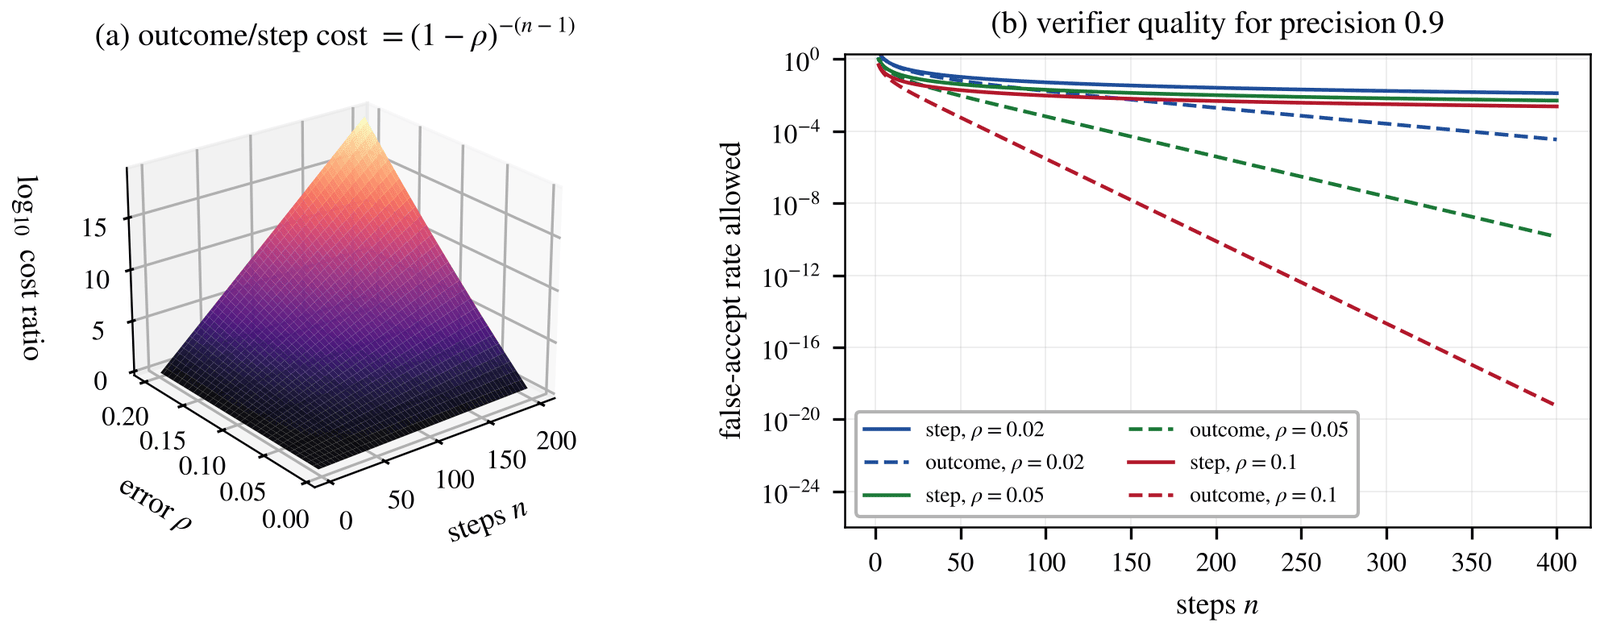
\includegraphics[width=0.98\textwidth]{figures/fig_gating}
\caption{Theorem~\ref{thm:gating}. (a) The ratio $(1-\rho)^{-(n-1)}$ of the expected costs of outcome and step gating with perfect checks, on a logarithmic scale, for up to two hundred steps and error rates $\rho\le0.2$. (b) The false acceptance rate a check may have to reach precision $0.9$ with $\eta=0$: for step gating (solid lines and shaded bands between the sufficient and the necessary rate of part (iv)) it decreases like $1/n$, for outcome gating (dashed) like $(1-\rho)^{n}$.}
\label{fig:gating}
\end{figure*}

\begin{figure*}[t]
\centering
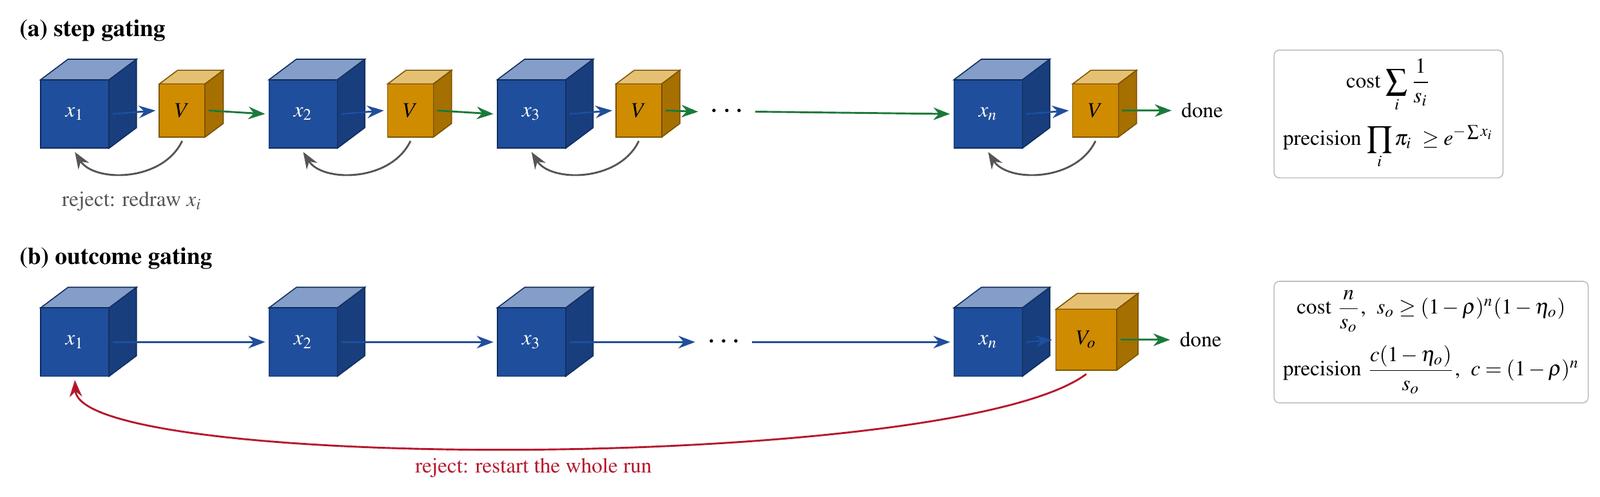
\includegraphics[width=0.94\textwidth]{figures/fig_gatingflow}
\caption{The two protocols of Theorem~\ref{thm:gating}. (a) Step gating: each step is generated and checked, and regenerated until accepted; the cost is $\sum1/s_{i}$ and the precision $\prod\pi_{i}\ge e^{-\sum x_{i}}$. (b) Outcome gating: the chain is generated to the end and checked once, and regenerated until accepted; the acceptance probability is at least $(1-\rho)^{n}(1-\eta_{o})$, the cost is $n/s_{o}$ and the precision $c(1-\eta_{o})/s_{o}$.}
\label{fig:gatingflow}
\end{figure*}

\begin{remark}[Relation to learning from outcomes]
Jia, Rakhlin and Xie proved that learning a policy from outcome rewards is statistically no harder than learning it from step rewards, up to polynomial factors in the horizon \cite{JRX25}. Theorem~\ref{thm:gating} is about a different cost, that of certifying a chain with checks that are already given, and the two results are compatible: a learner may extract as much from outcomes as from steps, while a certifier that sees only outcomes pays exponentially in retries and in the reliability its check must have. Rohatgi and coauthors observe the same amplification of verifier error along a generation from the side of sampling \cite{RSS25}.
\end{remark}

\section{Sound singularities}\label{sec:singularity}

\subsection{Singular chains}

Let the chain of Section~\ref{sec:chains} run forever: step $n\ge1$ costs $g_{n}$ per candidate to generate and $a_{n}$ per run to check, is incorrect with probability $\rho_{n}$, and is checked by $r_{n}$ runs of a sharp check of soundness $\eps$, all steps independent. The total cost is $T_{\infty}=\sum_{n}T_{n}$ and $F$ counts the steps whose kept candidate is incorrect.

\begin{definition}\label{def:singular}
The chain is \emph{singular} if $\EE\,T_{\infty}<\infty$, and \emph{sound} if $F<\infty$ almost surely.
\end{definition}

If cost is time, a singular chain completes infinitely many improvements in finite expected time, which is the vertical asymptote of the explosion literature \cite{Goo66,Ord26}; if cost is compute or energy, it completes them on a finite budget. Soundness asks that only finitely many of the improvements be wrong, so that from some step on the system is correct.

\begin{proof}[Proof of Theorem~\ref{thm:E}]
Put $\gamma=1-\bar\rho$. By Lemma~\ref{lem:onestep}, $g_{n}+a_{n}r_{n}\le\EE\,T_{n}\le(g_{n}+a_{n}r_{n})/\gamma$ and $\rho_{\ast}\eps^{r_{n}}\le\pi_{n}\le\eps^{r_{n}}/\gamma$. So $\EE\,T_{\infty}<\infty$ if and only if $\sum(g_{n}+a_{n}r_{n})<\infty$, and $\sum\pi_{n}<\infty$ if and only if $\sum\eps^{r_{n}}<\infty$.

(i) Let $E_{n}$ be the event that the candidate kept at step $n$ is incorrect, so $F=\sum\ind_{E_{n}}$ and the $E_{n}$ are independent with $\PR(E_{n})=\pi_{n}<1$. If $\sum\pi_{n}<\infty$, then $\EE F<\infty$, so $F<\infty$ almost surely (this is the first Borel--Cantelli lemma \cite{Bor09,Dur19}), and $\PR(F=0)=\prod_{n}(1-\pi_{n})>0$, because a product of factors in $(0,1]$ converges to a positive limit when the sum of the complements converges. If $\sum\pi_{n}=\infty$, the second Borel--Cantelli lemma for independent events gives $\PR(E_{n}\text{ infinitely often})=1$, so $F=\infty$ almost surely and $\PR(F=0)=0$.

(ii) If every $r_{n}\ge1$, then $\sum a_{n}r_{n}\ge\sum a_{n}$, so a singular chain needs $\sum g_{n}<\infty$ and $\sum a_{n}<\infty$; conversely $r_{n}=1$ gives $\EE\,T_{\infty}\le\sum(g_{n}+a_{n})/\gamma<\infty$.

(iii) A sound singular chain needs $\sum g_{n}<\infty$, $\sum a_{n}r_{n}<\infty$ and $\sum\eps^{r_{n}}<\infty$. The last forces $r_{n}\ge1$ for all large $n$, so $\sum a_{n}<\infty$, and Proposition~\ref{prop:integer} (applied to the tail on which $a_{n}\le1$) gives $\sum a_{n}\log(1/a_{n})<\infty$. Conversely, under the three conditions, the schedule $r_{n}=\lceil\log(1/a_{n})/L\rceil$ of Proposition~\ref{prop:integer}, raised to at least one run, has $\sum a_{n}r_{n}<\infty$ and $\sum\eps^{r_{n}}<\infty$.
\end{proof}

The theorem has a simple form: the chain can reach the asymptote if the steps get cheap fast enough, and it can reach it soundly if they get cheap fast enough to pay for the entropy. Since $a\log(1/a)\ge a$ for $a\le1/e$, the second condition is strictly stronger, and the next corollary shows that the gap between them is not empty.

\begin{corollary}[The soundness gap]\label{cor:gap}
Let $a_{n}=1/(n\log^{\beta}n)$ for $n\ge3$, with $\sum g_{n}<\infty$. A singular chain with every step checked exists if and only if $\beta>1$, and a sound singular chain exists if and only if $\beta>2$. For $1<\beta\le2$ every singular chain keeps infinitely many incorrect modifications almost surely.
\end{corollary}

\begin{proof}
The series $\sum1/(n\log^{c}n)$ converges if and only if $c>1$, by Cauchy's condensation test: its terms decrease, and $2^{k}$ times the term at $n=2^{k}$ is $(k\log2)^{-c}$ (Appendix~\ref{app:condensation}). So $\sum a_{n}<\infty$ if and only if $\beta>1$. For the entropy, $\log(1/a_{n})=\log n+\beta\log\log n$, which lies between $\log n$ and $2\log n$ for all large $n$, so $a_{n}\log(1/a_{n})$ lies between $1/(n\log^{\beta-1}n)$ and twice it, and $\sum a_{n}\log(1/a_{n})<\infty$ if and only if $\beta-1>1$. Theorem~\ref{thm:E} concludes; the last claim is part (i), since a singular chain with $1<\beta\le2$ cannot have $\sum\eps^{r_{n}}<\infty$.
\end{proof}

Figure~\ref{fig:price}(b) shows the condensed partial sums of the two series for three values of $\beta$.

\subsection{Power laws}

The case that matters for growth models is a power law, $a_{n}=n^{-p}$ with $p>1$. Then $A=\zeta(p)$, the profile has entropy
\[
H(p)=\log\zeta(p)+p\,\frac{-\zeta'(p)}{\zeta(p)},
\]
by \eqref{eq:AH}, and $\sum a_{n}\log(1/a_{n})=p\sum n^{-p}\log n<\infty$ for every $p>1$. So every power law admits a sound singularity, and the question is its price.

\begin{proposition}[Price of a power-law takeoff]\label{prop:powerlaw}
As $p\to1^{+}$,
\[
\begin{aligned}
H(p)&=\frac1{p-1}+\log\frac1{p-1}+O(1),\\
\frac{\Vs(\theta)}{A}&=\frac1{(p-1)L}+O\Bigl(\log\frac1{p-1}\Bigr),
\end{aligned}
\]
for fixed $\theta\in(0,1]$ and $\eps$, so that $\Vs(\theta)=\frac{1}{(p-1)^{2}L}\bigl(1+O((p-1)\log\frac1{p-1})\bigr)$.
\end{proposition}

\begin{proof}
Put $t=p-1$. Comparing the decreasing function $x^{-p}$ with its integral, $1/t=\int_{1}^{\infty}x^{-p}\,dx\le\zeta(p)\le1+1/t$. The function $f(x)=x^{-p}\log x$ vanishes at $1$, increases on $[1,e^{1/p}]$ and decreases afterwards, with maximum $1/(pe)$, so $\bigl|\sum_{n\ge1}f(n)-\int_{1}^{\infty}f\bigr|\le1/(pe)$ (Appendix~\ref{app:zeta}); and $\int_{1}^{\infty}x^{-p}\log x\,dx=1/t^{2}$. Hence $-\zeta'(p)=1/t^{2}+O(1)$ and
\[
\frac{-p\zeta'(p)}{\zeta(p)}=\frac{(1+t)(t^{-2}+O(1))}{t^{-1}(1+O(t))}=\frac1t+O(1)
\]
and $\log\zeta(p)=\log\frac1t+O(t)$.
This is the first formula. The second follows from Theorem~\ref{thm:A}, Proposition~\ref{prop:infinite} and $A=1/t+O(1)$.
\end{proof}

The constant term is $1-\gamma_{E}$, where $\gamma_{E}$ is Euler's constant, as the Laurent expansion $\zeta(p)=1/t+\gamma_{E}+O(t)$ shows; at $p=1.1$ the three terms give $12.725$ against the exact $H=12.745$. So the cheapest sound takeoff along a power law near the critical exponent costs, per unit of the cost of one run per step, about $1/((p-1)L)$, and in total about $1/((p-1)^{2}L)$: the soundness of the takeoff is paid for with one extra factor $1/(p-1)$ (Fig.~\ref{fig:price}(a)).

\begin{figure*}[t]
\centering
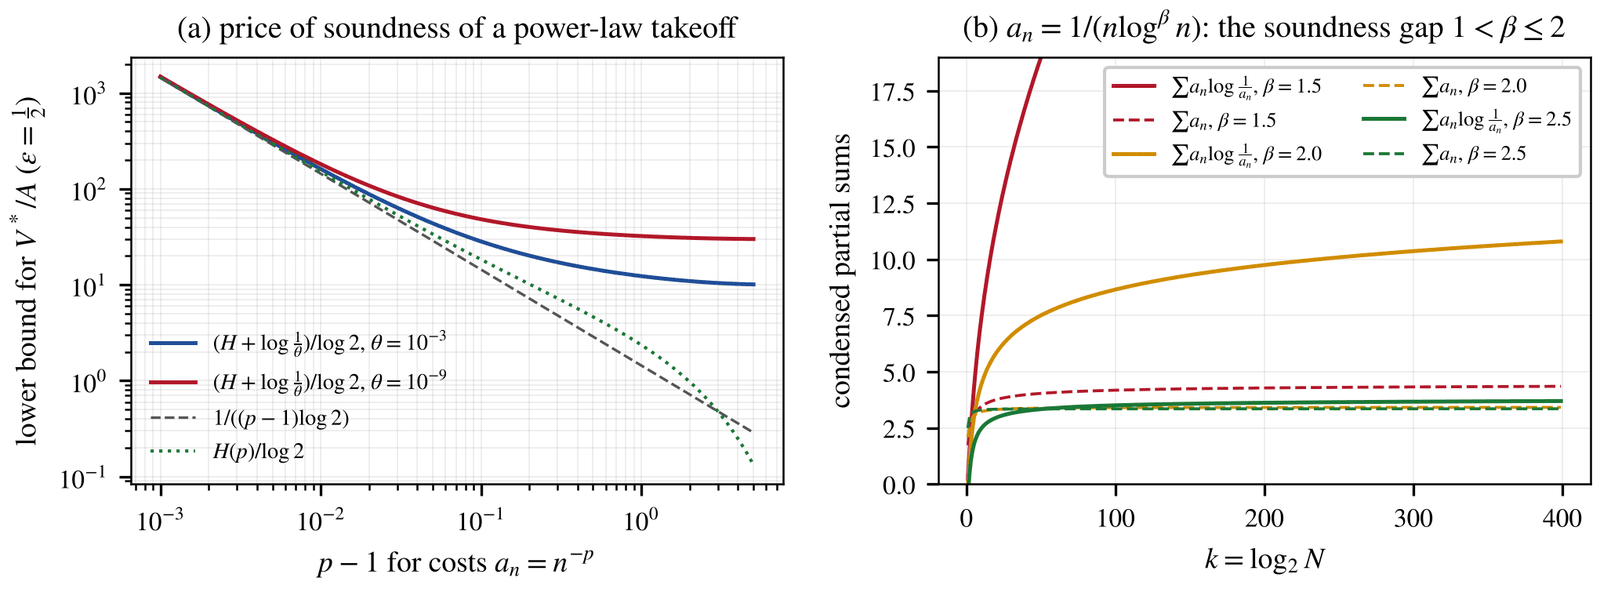
\includegraphics[width=0.98\textwidth]{figures/fig_price}
\caption{(a) The lower bound $(H(p)+\log\frac1\theta)/\log2$ for $\Vs/A$ along the power laws $a_{n}=n^{-p}$, with $\eps=\frac12$ and $\theta=10^{-3}$, $10^{-9}$; as $p\to1$ it approaches $1/((p-1)\log2)$ (dashed), the term that dominates the entropy (dotted). (b) The soundness gap of Corollary~\ref{cor:gap}: condensed partial sums of $\sum a_{n}$ (dashed) and $\sum a_{n}\log\frac1{a_{n}}$ (solid) for $a_{n}=1/(n\log^{\beta}n)$. At $\beta=1.5$ the cost converges and the entropy diverges; at $\beta=2$ the entropy still diverges, like $\log\log N$; at $\beta=2.5$ both converge.}
\label{fig:price}
\end{figure*}

\subsection{Polynomial checks and the phase diagram}

With checks of order $s$, Corollary~\ref{cor:dualcases}(ii) replaces the entropy condition by $\sum a_{n}^{1/(1+s)}<\infty$.

\begin{corollary}[Phase diagram]\label{cor:phase}
Let $a_{n}=n^{-p}$ and $\sum g_{n}<\infty$. A singular chain with every step checked exists if and only if $p>1$. With exponential checks a sound one exists for every $p>1$; with checks of order $s$ a sound one exists if and only if $p>1+s$. For geometric costs $a_{n}=c^{n}$, $0<c<1$, a sound singular chain exists for every $s$.
\end{corollary}

\begin{proof}
The series $\sum n^{-p/(1+s)}$ converges if and only if $p>1+s$, and the series $\sum c^{n/(1+s)}$ converges for every $s$. For the singular part, a check of order $s$ with $\delta_{n}=1$ costs $a_{n}$.
\end{proof}

Figure~\ref{fig:regimes} draws the phase diagram. Below the line $p=1$ there is no singularity at all; between $p=1$ and $p=1+s$ there are singular chains and all of them are unsound; above $p=1+s$ there are sound ones. Exponential checks are the edge $s=0$ of the diagram, and the logarithmic family of Corollary~\ref{cor:gap} sits on the line $p=1$, where the finer scale $\beta$ splits it again.

\begin{figure*}[t]
\centering
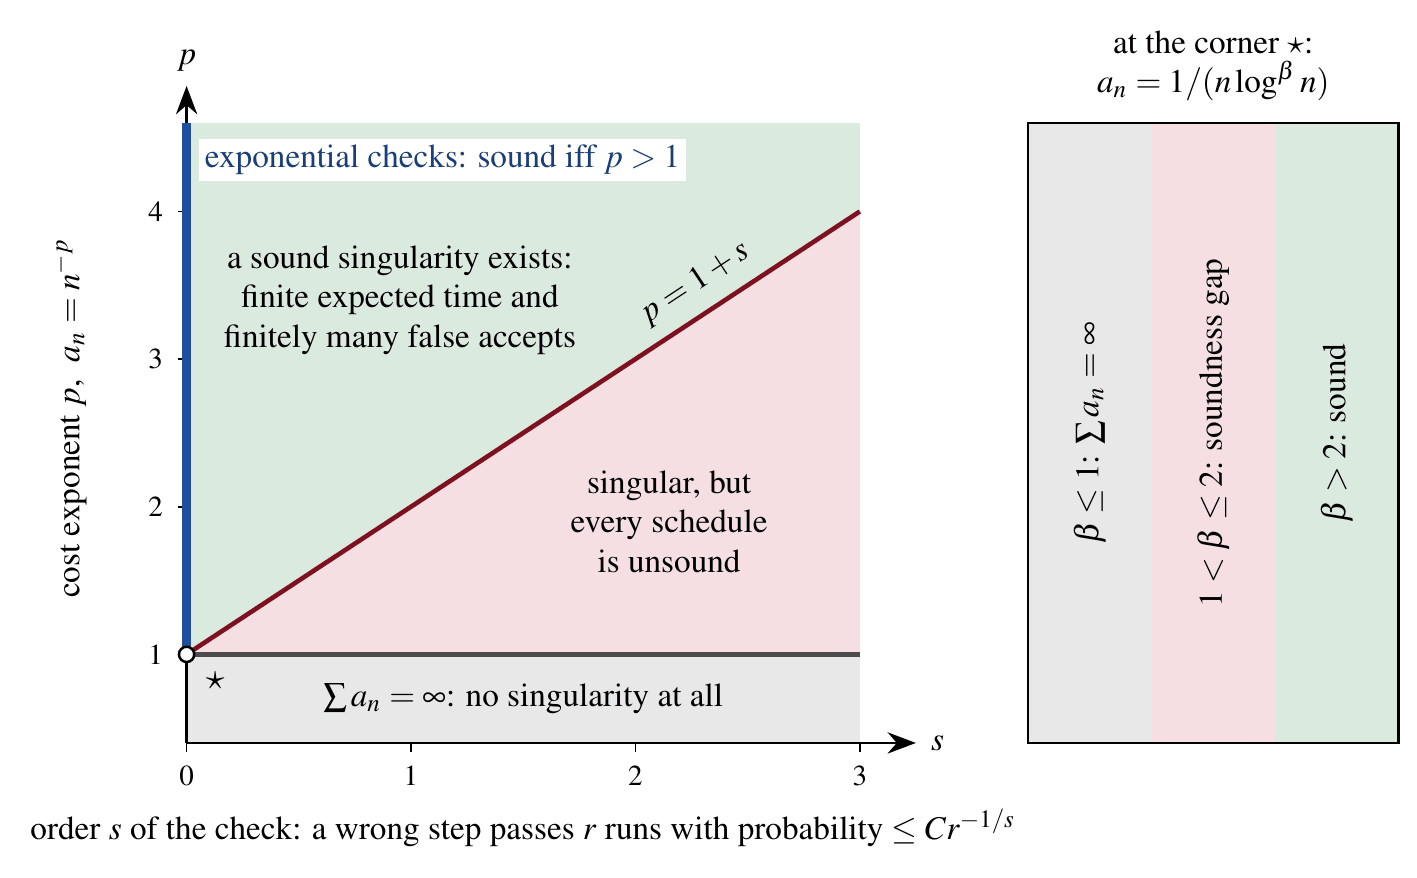
\includegraphics[width=0.86\textwidth]{figures/fig_regimes}
\caption{The phase diagram of Corollary~\ref{cor:phase} in the plane of the polynomial order $s$ of the checks and the exponent $p$ of the cost law $a_{n}=n^{-p}$. No singularity for $p\le1$; singular chains that are all unsound for $1<p\le1+s$; sound singular chains for $p>1+s$. The axis $s=0$ is the case of exponential checks, sound for every $p>1$. The panel at the corner refines the line $p=1$ by the logarithmic family $a_{n}=1/(n\log^{\beta}n)$ of Corollary~\ref{cor:gap}.}
\label{fig:regimes}
\end{figure*}

\section{Checking without knowing the future}\label{sec:online}

The schedules of Sections~\ref{sec:entropy} to~\ref{sec:singularity} are computed from the whole cost profile: the number of runs of the $i$-th check depends on $A$ and on every other cost. A self-improving system does not know its future modifications. When the $n$-th candidate arrives, only $a_{1},\dots,a_{n}$ are known, and the number of runs of its check must be fixed then. This section shows that such a system loses almost nothing: the entropy law survives with an additive term that grows like the logarithm of the logarithm of the dynamic range, and that term cannot be removed.

\subsection{Online schedules}

An \emph{online schedule} is a rule that assigns to each finite sequence $(a_{1},\dots,a_{n})$ of positive costs a number $r_{n}\in\NN$ of runs for the last candidate. Applied to a sequence $(a_{n})_{n\ge1}$, finite or infinite, it produces the schedule $(r_{n})$, and $r_{n}$ does not depend on $a_{n+1},a_{n+2},\dots$. The rule is \emph{$\theta$-sound} if $\sum_{n}\eps^{r_{n}}\le\theta$ for every sequence of positive costs. Write
\[
S_{n}=a_{1}+\dots+a_{n},\qquad u_{n}=\log\frac{S_{n}}{a_{1}},\qquad w_{n}=\frac{a_{n}/S_{n}}{2(1+u_{n})^{2}},
\]
so that $u_{1}=0$, $u_{n}$ is nondecreasing and $w_{1}=\frac12$. On the first $N$ candidates write $A_{N}=S_{N}$, $p^{(N)}=(a_{n}/A_{N})_{n\le N}$, $V_{N}=\sum_{n\le N}a_{n}r_{n}$ and $\Vs_{N}(\theta)$ for the offline optimum of Theorem~\ref{thm:A}.

\begin{mainthm}[Online entropy law]\label{thm:G}
Let $0<\eps<1$ and $0<\theta\le1$. The online schedule
\begin{equation}\label{eq:onlinerule}
r_{n}=\Bigl\lceil\frac1L\log\frac{1}{\theta w_{n}}\Bigr\rceil=\Bigl\lceil\frac1L\log\frac{2(1+u_{n})^{2}S_{n}}{\theta a_{n}}\Bigr\rceil
\end{equation}
is $\theta$-sound, and for every $N$
\begin{equation}\label{eq:onlineupper}
\begin{aligned}
V_{N}\le{}&\frac{A_{N}}{L}\Bigl(H(p^{(N)})+\log\frac1\theta\Bigr)\\
&+\frac{A_{N}}{L}\Bigl(\log2+2\log\Bigl(1+\log\frac{A_{N}}{a_{1}}\Bigr)\Bigr)+A_{N}.
\end{aligned}
\end{equation}
Conversely, on the doubling costs $a_{n}=2^{n-1}$ every $\theta$-sound online schedule satisfies, for infinitely many $N$,
\begin{equation}\label{eq:onlinelower}
V_{N}-\Vs_{N}(\theta)\ \ge\ \frac{A_{N}}{2L}\log\log_{2}\Bigl(1+\frac{A_{N}}{a_{1}}\Bigr)-\Bigl(1+\frac{2\log2}{L}\Bigr)A_{N}.
\end{equation}
\end{mainthm}

Together with the lower bound of Theorem~\ref{thm:A}, \eqref{eq:onlineupper} says that the price of not knowing the future is at most $(A_{N}/L)(\log2+2\log(1+\log(A_{N}/a_{1})))+A_{N}$, and \eqref{eq:onlinelower} says that a term of order $(A_{N}/L)\log\log(A_{N}/a_{1})$ must be paid by every online rule on some sequences. The two bounds differ by a factor of four in the leading term. The dynamic range $A_{N}/a_{1}$ enters only through a double logarithm: a system whose total checking cost grows by a factor $10^{100}$ over its first candidate pays at most $2\log(1+100\log10)\approx10.9$ extra runs per unit of cost, measured in units of $L$.

\begin{corollary}[Sound singularities without foresight]\label{cor:onlinesing}
If $\sum_{n}a_{n}<\infty$ and $\sum_{n}a_{n}\log(1/a_{n})<\infty$, the online schedule \eqref{eq:onlinerule} is $\theta$-sound and has finite total cost
\[
V\le\frac{A}{L}\Bigl(H(p)+\log\frac1\theta+\log2+2\log\Bigl(1+\log\frac{A}{a_{1}}\Bigr)\Bigr)+A .
\]
\end{corollary}

So the criterion of Theorem~\ref{thm:E} does not need an oracle. A chain that only knows its past costs reaches a sound singularity whenever any chain does, and the rule that achieves it is the same for every sequence.

\subsection{Proofs}

The proof rests on two elementary facts, both proved in Lean (Appendix~\ref{app:checks}).

\begin{lemma}[Telescoping]\label{lem:telescope}
For $0\le x\le y$, $\dfrac{y-x}{(1+y)^{2}}\le\dfrac1{1+x}-\dfrac1{1+y}$. Hence for a nondecreasing sequence $0\le u_{1}\le u_{2}\le\cdots$,
\[
\sum_{n=2}^{N}\frac{u_{n}-u_{n-1}}{(1+u_{n})^{2}}\ \le\ \frac1{1+u_{1}}-\frac1{1+u_{N}}.
\]
\end{lemma}

\begin{proof}
The right side of the first inequality is $(y-x)/((1+x)(1+y))$, and $(1+x)\le(1+y)$. Summing gives a telescoping series.
\end{proof}

\begin{lemma}[Share of the newest cost]\label{lem:share}
For $0<s\le t$, $1-s/t\le\log(t/s)$. In particular $a_{n}/S_{n}=1-S_{n-1}/S_{n}\le u_{n}-u_{n-1}$ for $n\ge2$.
\end{lemma}

\begin{proof}
This is $1-1/x\le\log x$ at $x=t/s$, which is $\log y\le y-1$ at $y=1/x$. For the second statement take $s=S_{n-1}$, $t=S_{n}$ and note $\log(S_{n}/S_{n-1})=u_{n}-u_{n-1}$.
\end{proof}

\begin{proof}[Proof of Theorem~\ref{thm:G}]
\emph{Soundness.} By Lemmas~\ref{lem:share} and~\ref{lem:telescope},
\[
\begin{aligned}
\sum_{n=1}^{N}w_{n}&=\frac12+\frac12\sum_{n=2}^{N}\frac{a_{n}/S_{n}}{(1+u_{n})^{2}}\le\frac12+\frac12\sum_{n=2}^{N}\frac{u_{n}-u_{n-1}}{(1+u_{n})^{2}}\\
&\le\frac12+\frac12\Bigl(1-\frac1{1+u_{N}}\Bigr)<1
\end{aligned}
\]
for every $N$ and every sequence of positive costs. Since $w_{n}\le\frac12<1$ and $\theta\le1$, the number inside the ceiling of \eqref{eq:onlinerule} is positive and $\eps^{r_{n}}\le\theta w_{n}$. Hence $\sum_{n}\eps^{r_{n}}\le\theta\sum_{n}w_{n}\le\theta$, and $r_{n}$ depends only on $a_{1},\dots,a_{n}$.

\emph{Cost.} From $r_{n}<\frac1L\log\frac1{\theta w_{n}}+1$,
\[
\begin{aligned}
L\,V_{N}<{}&\sum_{n\le N}a_{n}\Bigl(\log\frac1\theta+\log2+2\log(1+u_{n})\Bigr)\\
&+\sum_{n\le N}a_{n}\log\frac{S_{n}}{a_{n}}+L\,A_{N}.
\end{aligned}
\]
For $n\le N$ we have $S_{n}\le A_{N}$, so $\log(S_{n}/a_{n})\le\log(A_{N}/a_{n})$ and $u_{n}\le\log(A_{N}/a_{1})$. Since $\sum_{n\le N}a_{n}\log(A_{N}/a_{n})=A_{N}H(p^{(N)})$, \eqref{eq:onlineupper} follows.

\emph{Lower bound.} Fix a $\theta$-sound online rule and apply it to the infinite sequence $a_{n}=2^{n-1}$. Its decisions on the first $N$ candidates are those it takes on the finite sequence $(a_{1},\dots,a_{N})$. Put $v_{n}=\eps^{r_{n}}/\theta$, so $\sum_{n}v_{n}\le1$. Then $v_{N}\le1/N$ for infinitely many $N$: otherwise $v_{N}>1/N$ for all large $N$ and $\sum v_{N}$ would diverge with the harmonic series. For such $N$, $r_{N}L\ge\log(N/\theta)$, and $r_{n}L\ge\log(1/\theta)$ for every $n$ because $\eps^{r_{n}}\le\theta$. Hence
\[
L\,V_{N}\ \ge\ A_{N}\log\frac1\theta+a_{N}\log N .
\]
On the other side, $p^{(N)}_{n}=2^{n-1}/(2^{N}-1)\ge2^{n-1-N}$, so
\[
\begin{aligned}
H(p^{(N)})&\le\log2\sum_{n=1}^{N}(N-n+1)\,p^{(N)}_{n}\\
&=\log2\cdot\frac{2^{N+1}-N-2}{2^{N}-1}\le2\log2,
\end{aligned}
\]
by the identity $\sum_{k=1}^{N}k2^{-k}=2-(N+2)2^{-N}$, and Theorem~\ref{thm:A} gives $L\,\Vs_{N}(\theta)\le A_{N}(2\log2+\log\frac1\theta)+LA_{N}$. Subtracting, and using $a_{N}=2^{N-1}\ge A_{N}/2$ and $N=\log_{2}(1+A_{N}/a_{1})$, gives \eqref{eq:onlinelower}.
\end{proof}

\begin{proof}[Proof of Corollary~\ref{cor:onlinesing}]
Soundness is that of Theorem~\ref{thm:G}. For the cost, the argument of the upper bound with $A$ in place of $A_{N}$ bounds every partial sum $V_{N}$ by the right side, since $S_{n}\le A$ for all $n$ and $\sum_{n\le N}a_{n}\log(A/a_{n})\le AH(p)$. The right side is finite because $AH(p)=A\log A+\sum_{n}a_{n}\log(1/a_{n})$.
\end{proof}

\subsection{Universal codes}

Theorem~\ref{thm:G} is the schedule counterpart of the universal codes for the integers. Elias constructed prefix codes whose length for the integer $m$ is $\log m+O(\log\log m)$ without knowledge of the distribution of $m$ \cite{Eli75}, and Rissanen derived from them a universal prior whose code length $\log^{\ast}m$ is optimal up to the iterated logarithms \cite{Ris83}. Here the role of the integer is played by the ratio $S_{n}/a_{1}$, the weight $w_{n}$ is a code length in disguise, and the double logarithm of \eqref{eq:onlineupper} is the price of the second level of the Elias code. The constant $2$ in front of it can be lowered to $1+\delta$ for every $\delta>0$ by replacing $(1+u_{n})^{2}$ with $c_{\delta}(1+u_{n})(1+\log(1+u_{n}))^{1+\delta}$, as in the Elias $\omega$ code; the lower bound \eqref{eq:onlinelower} shows that no rule removes the double logarithm.

Figure~\ref{fig:online} shows the rule at work. On random profiles its cost stays within the band of Theorem~\ref{thm:G}, and on the doubling sequence the excess over the offline optimum grows like $\log\log$ of the dynamic range, as the lower bound requires.

\begin{figure*}[t]
\centering
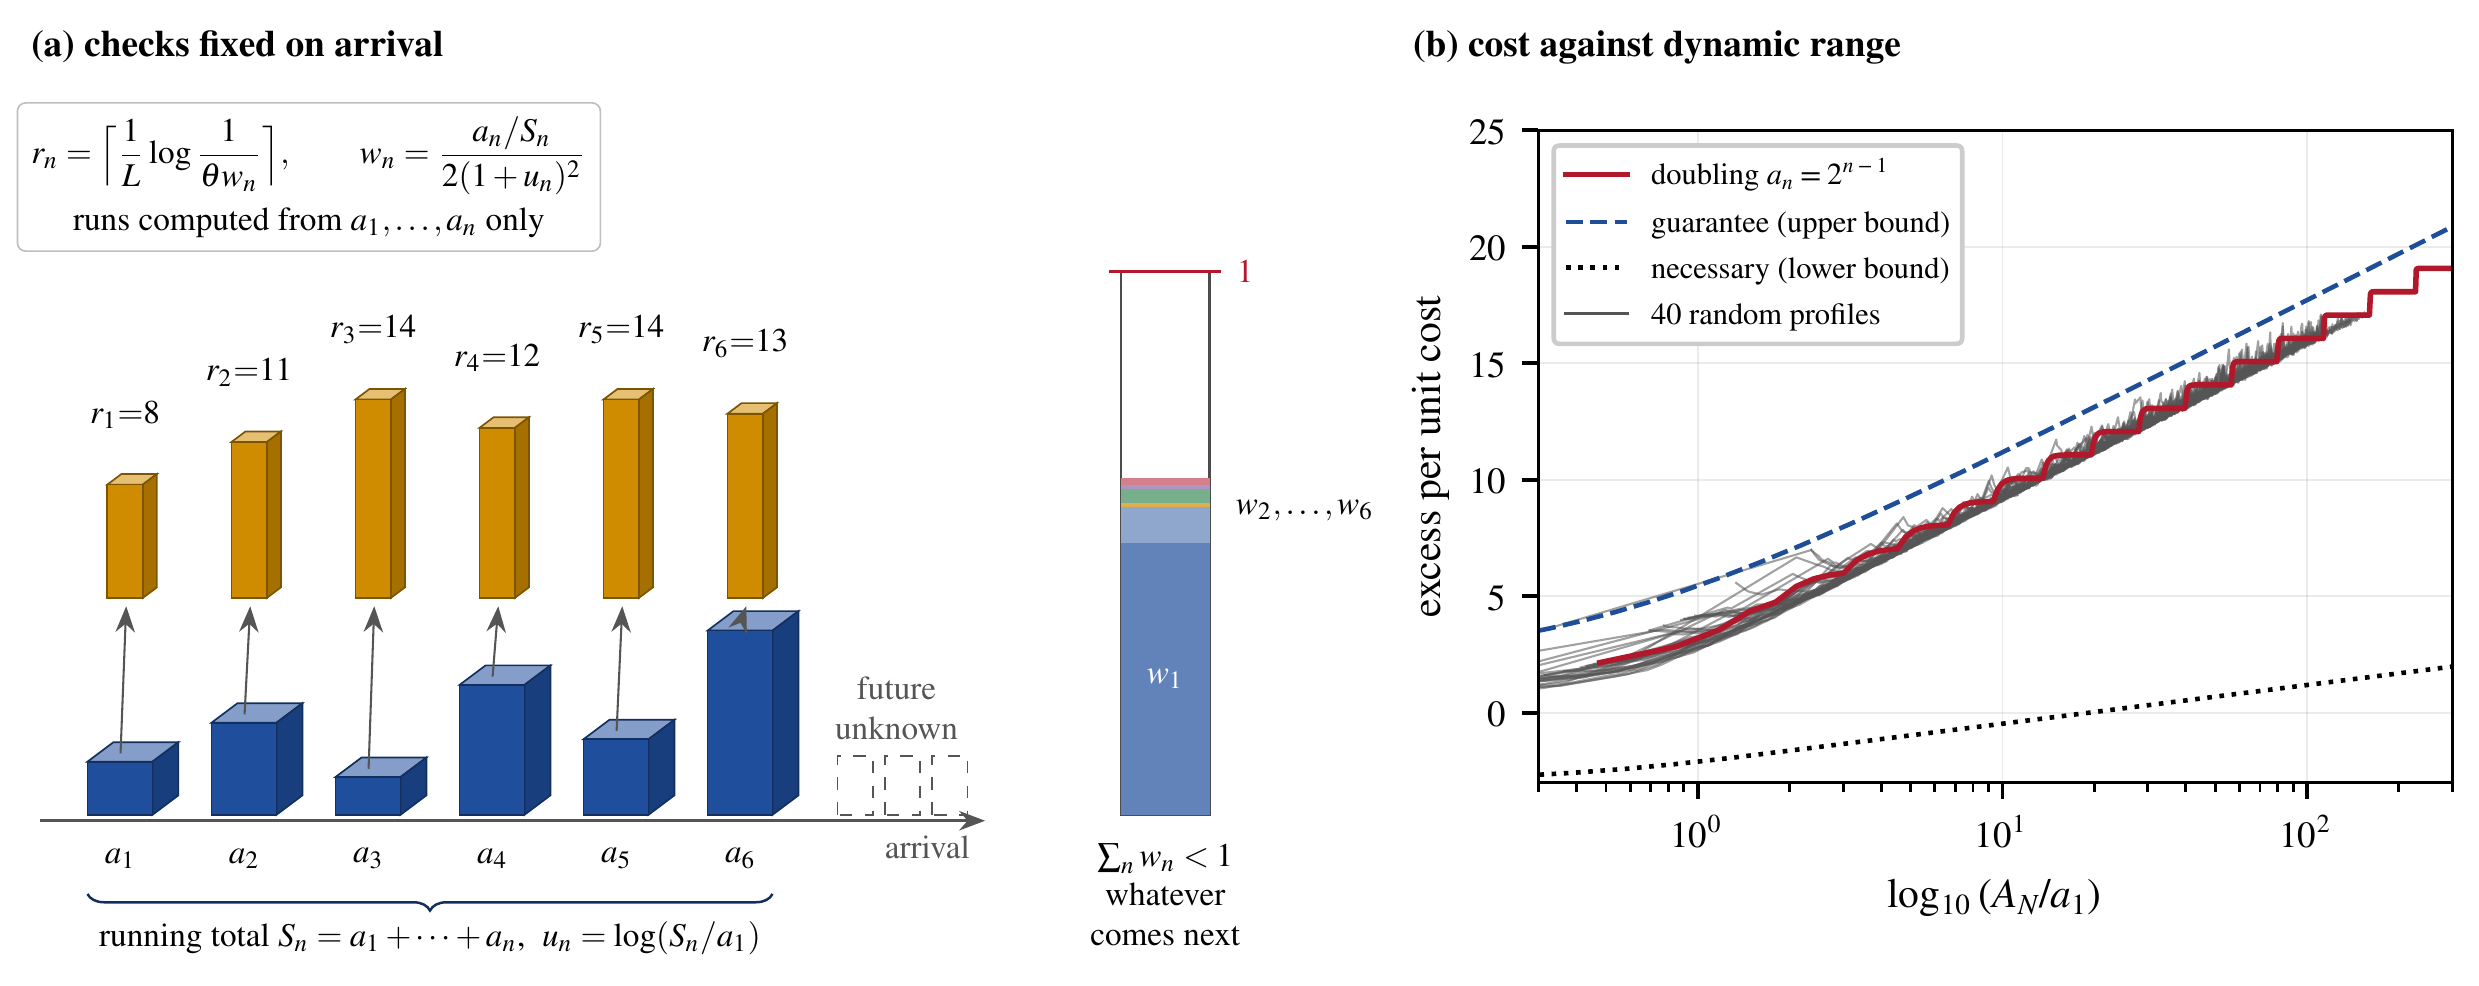
\includegraphics[width=0.98\textwidth]{figures/fig_online}
\Description{Diagram of candidates arriving one at a time with run numbers computed from the running total, and curves of the excess of the online rule over the offline bound with its guarantee.}
\caption{The online entropy law. (a) Candidates arrive one at a time; the $n$-th check is given $r_{n}$ runs computed from the running total $S_{n}$ alone, and the weights $w_{n}$ never sum to more than one, whatever comes next. (b) The excess $(V_{N}-\frac{A_{N}}{L}(H+\log\frac1\theta))/A_{N}$ of the online rule over the offline lower bound, for the doubling sequence $a_{n}=2^{n-1}$ (red) and for forty random profiles with log-normal costs (grey), against $\log_{10}(A_{N}/a_{1})$ on a logarithmic axis, with $\eps=\frac12$ and $\theta=10^{-6}$. The dashed curve is the guarantee $(\log2+2\log(1+\log(A_{N}/a_{1})))/L+1$ of \eqref{eq:onlineupper}, and the dotted curve is the necessary excess $\frac1{2L}\log\log_{2}(1+A_{N}/a_{1})-1-\frac{2\log2}{L}$ of \eqref{eq:onlinelower}.}
\label{fig:online}
\end{figure*}

\section{Subagents, cascades and the moves of a proof}\label{sec:agents}

A working BLLM is not one generator and one check. A coordinator hands parts of a problem to subagents, each subagent proposes candidates by its own method, and the candidates meet checks of very different cost: a test that runs in a millisecond, a randomized identity test, a full proof checker. This section proves the two laws that govern such a system. Splitting the work among subagents costs nothing, provided each receives a share of the budget proportional to its total cost, and a misallocated budget is charged exactly a Kullback--Leibler divergence (Theorem~\ref{thm:H}). Cheap unreliable checks placed before an exact one make the exact check paid, up to a logarithmic premium, only on the correct candidates (Theorem~\ref{thm:cascade}). The section ends with the six moves by which the subagents of Section~\ref{sec:cases} propose candidates.

\subsection{Subagents}

Partition the candidates into groups $G_{1},\dots,G_{m}$, one for each subagent. Write $A_{k}=\sum_{i\in G_{k}}a_{i}$, $P_{k}=A_{k}/A$ for the share of the $k$-th subagent and $p^{(k)}=(a_{i}/A_{k})_{i\in G_{k}}$ for its own cost profile. A coordinator gives the $k$-th subagent a budget $\theta_{k}>0$ with $\Theta=\sum_{k}\theta_{k}\le\theta$, and the subagent schedules its checks with any $\theta_{k}$-sound schedule. The union of the schedules is $\theta$-sound, since the expected numbers of false acceptances add.

\begin{mainthm}[Subagents]\label{thm:H}
\begin{enumerate}[label=\textup{(\roman*)},leftmargin=2.2em,itemsep=1pt]
\item \emph{Chain rule.} $H(p)=H(P)+\sum_{k}P_{k}H(p^{(k)})$.
\item \emph{Price of a split.} The sum over the subagents of the lower bounds of Theorem~\ref{thm:A} for their groups exceeds the lower bound for the whole profile by exactly
\begin{equation}\label{eq:splitprice}
\frac{A}{L}\Bigl(D(P\,\|\,q)+\log\frac{\theta}{\Theta}\Bigr),\qquad q_{k}=\frac{\theta_{k}}{\Theta},
\end{equation}
where $D$ is the Kullback--Leibler divergence. It vanishes if and only if $\theta_{k}=\theta P_{k}$ for every $k$.
\item \emph{Coordination by one number.} If $\theta_{k}=\theta P_{k}$, the optimal schedule of Theorem~\ref{thm:A} computed by the $k$-th subagent from its own costs and the single number $\theta P_{k}$ coincides on $G_{k}$ with the optimal schedule of the whole profile. The union is $\theta$-sound and costs at most $\frac AL(H(p)+\log\frac1\theta)+A$.
\item \emph{Hierarchies.} For a tree of subagents in which every node passes to each child the share of its own budget proportional to the child's total cost, the schedule at the leaves is the optimal flat schedule, and
\begin{equation}\label{eq:treeentropy}
A\,H(p)=\sum_{v}A_{v}\,H(P^{v}),
\end{equation}
the sum over the internal nodes $v$ of the tree, where $A_{v}$ is the total cost below $v$ and $P^{v}$ the distribution of $A_{v}$ among the children of $v$.
\end{enumerate}
\end{mainthm}

\begin{proof}
(i) For $i\in G_{k}$, $\log(A/a_{i})=\log(A/A_{k})+\log(A_{k}/a_{i})$; multiply by $a_{i}$, sum over $i\in G_{k}$ and then over $k$, and divide by $A$.

(ii) The sum of the lower bounds of the groups is
\[
\frac1L\sum_{k}\Bigl(A_{k}H(p^{(k)})+A_{k}\log\frac1{\theta_{k}}\Bigr).
\]
By (i), subtracting $\frac AL(H(p)+\log\frac1\theta)$ leaves
\[
\begin{aligned}
&\frac1L\Bigl(\sum_{k}A_{k}\log\frac1{\theta_{k}}-A\,H(P)-A\log\frac1\theta\Bigr)\\
&\quad=\frac AL\sum_{k}P_{k}\log\frac{\theta P_{k}}{\theta_{k}}=\frac AL\Bigl(\sum_{k}P_{k}\log\frac{P_{k}}{q_{k}}+\log\frac\theta\Theta\Bigr).
\end{aligned}
\]
Both terms are nonnegative, the first by Gibbs' inequality (Lemma~\ref{lem:gibbs}), and they vanish together exactly when $q=P$ and $\Theta=\theta$, that is, when $\theta_{k}=\theta P_{k}$.

(iii) The ceiling schedule of the $k$-th group at budget $\theta P_{k}$ gives $i\in G_{k}$ the number of runs $\lceil\frac1L\log\frac{A_{k}}{\theta P_{k}a_{i}}\rceil=\lceil\frac1L\log\frac{A}{\theta a_{i}}\rceil$, which is the flat ceiling schedule; its soundness and cost are those of Theorem~\ref{thm:A}.

(iv) By induction on the depth, applying (iii) at the root and the induction hypothesis to each subtree with its proportional budget. The identity \eqref{eq:treeentropy} follows by applying (i) at every internal node.
\end{proof}

The theorem has a practical reading. A coordinator need not know the costs of the individual checks of its subagents, and a subagent need not know anything about the others: one number per subagent, its share $\theta P_{k}$ of the budget, is enough to reach the global optimum, and the identity \eqref{eq:treeentropy} says that the entropy tax is paid node by node along the tree of delegation, each node paying for the uncertainty of its own split. A coordinator that splits the budget evenly among $m$ subagents instead pays the extra $\frac AL D(P\,\|\,u)=\frac AL(\log m-H(P))$, where $u$ is uniform, and this is unbounded when a few subagents carry almost all the cost.

\subsection{Weak checks before strong ones}

Let a fraction $\rho\in(0,1)$ of the candidates be incorrect. A \emph{strong check} costs $c$ and is exact: it accepts the correct candidates and rejects the others, as a proof checker does on a formal proof. A \emph{weak check} costs $b$ per run, has perfect completeness and soundness $\eps$: a language model asked to find a flaw, a numerical test at random points, a type check. A \emph{cascade} with $r$ weak runs runs the weak check $r$ times on every candidate and the strong check on the candidates that pass them. It keeps exactly the correct candidates, whatever $r$, so its soundness is that of the strong check alone.

\begin{theorem}[Weak before strong]\label{thm:cascade}
If the weak check attains its soundness, the expected cost of a cascade with $r$ weak runs per candidate is
\[
E(r)=br+c(1-\rho)+c\rho\,\eps^{r},
\]
and for $b\le c\rho L$,
\begin{equation}\label{eq:cascade}
M\le\min_{r\in\NN}E(r)\le M+b,\qquad M=c(1-\rho)+\frac bL\Bigl(1+\log\frac{c\rho L}{b}\Bigr),
\end{equation}
the upper bound being attained up to $b$ by $r=\lceil\frac1L\log\frac{c\rho L}{b}\rceil$. Without weak checks the cost is $c$.
\end{theorem}

\begin{proof}
A correct candidate passes the $r$ weak runs and reaches the strong check; an incorrect one reaches it with probability $\eps^{r}$. This gives $E(r)$. Put $y=c\rho\eps^{r}$, so that $r=\frac1L\log\frac{c\rho}{y}$ and
\[
br+c\rho\eps^{r}-\frac bL\Bigl(1+\log\frac{c\rho L}{b}\Bigr)=\frac bL\Bigl(\frac{yL}{b}-1-\log\frac{yL}{b}\Bigr)\ge0
\]
by $\log x\le x-1$. This is the lower bound. For the upper bound let $x=\frac1L\log\frac{c\rho L}{b}\ge0$ and $r=\lceil x\rceil$. Then $br\le bx+b$ and $\eps^{r}\le\eps^{x}=b/(c\rho L)$, so $c\rho\eps^{r}\le b/L$.
\end{proof}

The strong check is thus paid on a fraction $1-\rho$ of the candidates, the correct ones, plus a premium logarithmic in $c/b$. When most proposals are wrong, as for a language model that guesses the next step of a hard proof, the saving is close to the factor $1/(1-\rho)$. With a proof checker of cost $c=1000$, a weak check of cost $b=1$ and soundness $\frac12$, and nine proposals in ten wrong, the best cascade runs nine weak checks per candidate and costs $110.8$ against $1000$; the lower bound is $110.7$.

The proof shows something more important than the saving. The soundness of the cascade does not depend on $\eps$: a weak check, however unreliable, can only remove candidates, never admit one. A learned critic may therefore be used freely as a filter, and only as a filter; the decision belongs to the exact check. The same holds with a randomized strong check of soundness $\eps_{s}$ given $r_{s}$ runs, whose false acceptances are bounded by $\rho\eps^{r}\eps_{s}^{r_{s}}\le\rho\eps_{s}^{r_{s}}$, so the weak runs may also be counted towards the budget of Theorem~\ref{thm:A} but are never needed for it.

\subsection{The moves of a proof}\label{ssec:moves}

The formal proofs of Section~\ref{sec:cases} are built from a small number of moves, used over and over. We name six, and the BLLM package of Section~\ref{sec:cases} has one subagent for each. A move is a way of generating candidates; it carries no authority of its own, and every candidate it produces meets the same checks, so Theorems~\ref{thm:A} to~\ref{thm:H} and~\ref{thm:cascade} apply to any mixture of moves.

\emph{Construction} produces an explicit object, a flow, a lattice, a cycle, a schedule, together with the statement that it has the required property, which is then checked. \emph{Strong then weak} proposes the strongest statement first and, when it is rejected, the next rung of a ladder of weakenings: a special case, a bounded range, a conditional form. Each rung is a candidate and enters the cost profile of Theorem~\ref{thm:A}. \emph{Residual} turns a partial success into a new goal, the part that remains unproved; it is the retry of Theorem~\ref{thm:B}, and when the corrections go on without end, as in a construction corrected to every order, whether the infinite sequence can be certified at finite cost is decided by Theorem~\ref{thm:E} and, without knowledge of the future corrections, by Corollary~\ref{cor:onlinesing}. \emph{Trivialization} specialises the parameters of a goal until it becomes a finite computation, which a kernel decides exactly, so that its check has soundness zero. \emph{Bypass} replaces a step by a result already kept in memory, whose check has been paid once. \emph{Blow-up} searches for a singular object or a counterexample.

\begin{remark}[Refutations carry no entropy tax]\label{rem:refutation}
A counterexample checked by exact evaluation needs one run, whatever the budget, because its check has soundness zero; so do the finite computations produced by trivialization and the results reused by bypass. In a mixed profile the entropy of Theorem~\ref{thm:A} is therefore the entropy of the candidates whose checks are randomized, with total cost $A_{\mathrm{rand}}$, and the exact checks add their cost once. A system that turns more of its work into exact checks lowers both $A_{\mathrm{rand}}$ and the entropy it pays on it.
\end{remark}

Figure~\ref{fig:agents} shows the arrangement: a coordinator, six subagents, a cascade of weak and strong checks, and a memory that stores every kept result as a note linked to the results it uses.

\begin{figure*}[t]
\centering
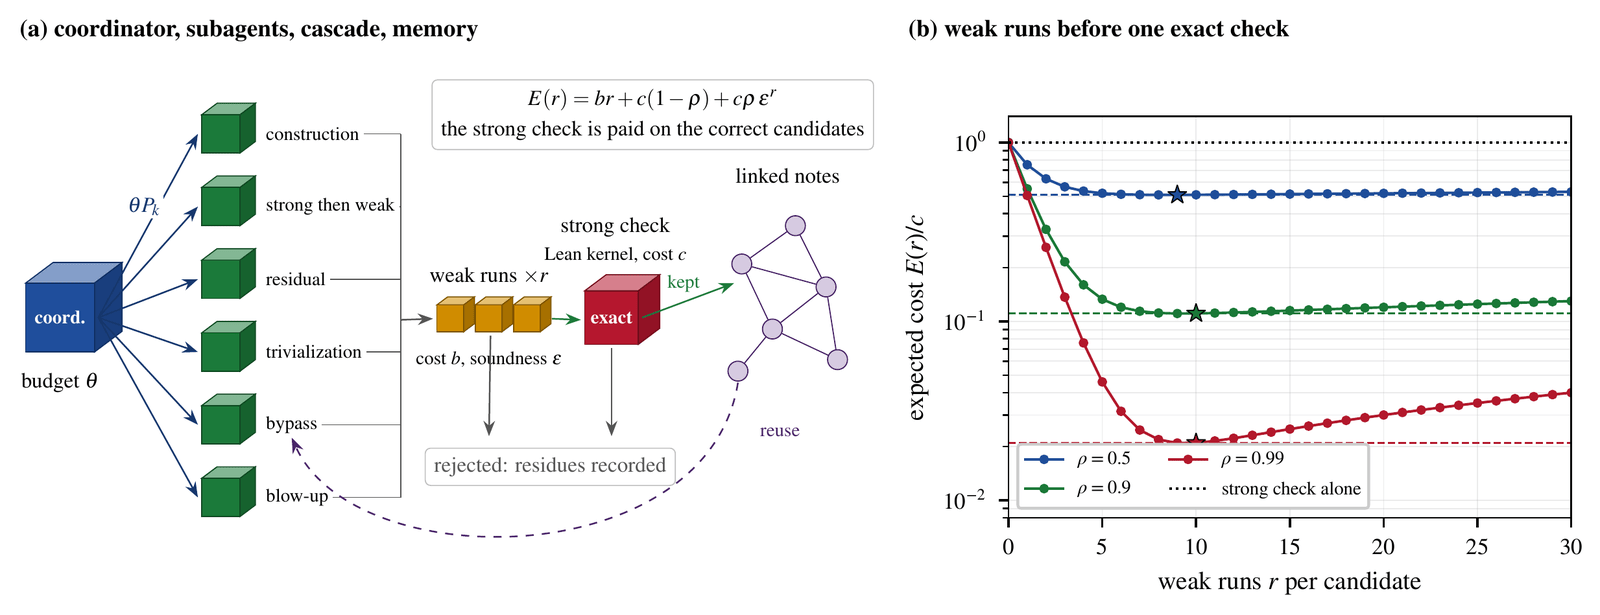
\includegraphics[width=0.98\textwidth]{figures/fig_agents}
\Description{A coordinator dividing the budget among six subagents with a cascade of weak runs and one strong check, and curves of the expected cost of a cascade against the number of weak runs.}
\caption{Subagents and cascades. (a) A coordinator passes to each of six subagents, one for each move of Section~\ref{ssec:moves}, the share $\theta P_{k}$ of the budget proportional to its total cost (Theorem~\ref{thm:H}); every candidate meets a cascade of $r$ weak runs and one exact strong check (Theorem~\ref{thm:cascade}), and the kept results are stored as linked notes that the bypass move reuses. (b) The expected cost $E(r)/c$ of a cascade against the number $r$ of weak runs, for $b/c=10^{-3}$, $\eps=\frac12$ and $\rho\in\{0.5,0.9,0.99\}$; stars mark the number of runs of Theorem~\ref{thm:cascade}, the lower bound $M$ of \eqref{eq:cascade} is dashed and the cost $1$ of the strong check alone dotted.}
\label{fig:agents}
\end{figure*}

\section{The gap between human and LLM thinking, and how a BLLM closes it}\label{sec:gap}

The theorems so far price the checking of what a proposer proposes. They are silent on the proposer itself, and a sound system whose proposer never reaches the right idea is sound and useless. Chen, Zhao and Cohan have measured how far the ideas of language models are from those of human researchers \cite{CZC26}.\footnote{Z.~Chen, Y.~Zhao and A.~Cohan, \emph{Measuring the gap between human and LLM research ideas}, preprint (1 July 2026), arXiv:2607.01233 \cite{CZC26}. For each of 11{,}683 papers of ICLR, ICML and NeurIPS (2023 to 2026) and of Nature Communications (2023 to 2025) they reconstruct a small set of prior works that likely inspired its core idea, ask a language model for a new idea from the titles and summaries of those works, and classify the human idea and the generated ones on two axes of seven classes: the kind of research opportunity (puzzle or contradiction, explanation gap, scope mismatch, evidence gap, bridge opportunity, failure or risk gap, resource bottleneck) and the kind of method (synthesis or unification, relaxing or extending the scope, robustification, formal derivation, empirical mapping, artifact or system, optimisation or search). They conclude that the range of the generated ideas is narrower than, and systematically shifted from, the human one. The shares used here are those of their Figure~3, read from the vector paths of the figure to $0.1$ percentage points and checked against the counts of their Table~11 and the distances of their Table~1.} Other measurements of the same gap, between the language a model produces and the reasoning it is asked for \cite{LCL25} and between human and model reasoning on naturalistic detective problems \cite{LG26}, point the same way. This section turns the measurement into a law: it computes, from the measured profiles, how many proposals a model needs to reach the kind of idea a problem calls for, proves the least possible number, and shows that a selector which learns from the checks reaches that least number.

\subsection{The gap law}

Ideas fall into $K$ classes. A problem needs an idea of class $j$ with probability $\pi_{j}$, its \emph{need}, and a proposer draws the classes of its proposals independently from a profile $q$ until it draws the needed class. The expected number of proposals is
\begin{equation}\label{eq:searchcost}
C(\pi,q)=\sum_{j}\pi_{j}\,\EE[\text{draws until }j]=\sum_{j}\frac{\pi_{j}}{q_{j}} .
\end{equation}
Write $S=\sum_{j}\sqrt{\pi_{j}}$, $r_{j}=\sqrt{\pi_{j}}/S$ and $H_{1/2}(\pi)=2\log S$, the R\'enyi entropy of order one half \cite{Ren61}; $\chi^{2}(r\|q)=\sum_{j}(r_{j}-q_{j})^{2}/q_{j}$ is the chi-squared divergence.

\begin{mainthm}[Gap law]\label{thm:I}
For every need $\pi$ and every profile $q$ with $q_{j}>0$,
\begin{enumerate}[label=\textup{(\roman*)},leftmargin=2.2em,itemsep=1pt]
\item $C(\pi,q)\ge S^{2}=e^{H_{1/2}(\pi)}$, with equality exactly at $q=r$, square-root sampling;
\item $C(\pi,q)=e^{H_{1/2}(\pi)}\bigl(1+\chi^{2}(r\|q)\bigr)$;
\item for every $\lambda\in(0,1]$ the mixture $q_{\lambda}=(1-\lambda)q+\lambda r$ has $C(\pi,q_{\lambda})\le e^{H_{1/2}(\pi)}/\lambda$, whatever $q$ is;
\item a proposer that copies the need, $q=\pi$, pays $K\ge S^{2}$, with equality only for the uniform need.
\end{enumerate}
\end{mainthm}

\begin{proof}
(i) By the Cauchy--Schwarz inequality,
\[
S=\sum_{j}\sqrt{\frac{\pi_{j}}{q_{j}}}\,\sqrt{q_{j}}\le\Bigl(\sum_{j}\frac{\pi_{j}}{q_{j}}\Bigr)^{1/2}\Bigl(\sum_{j}q_{j}\Bigr)^{1/2}=C(\pi,q)^{1/2},
\]
with equality if and only if $\sqrt{\pi_{j}/q_{j}}$ is proportional to $\sqrt{q_{j}}$, that is $q_{j}\propto\sqrt{\pi_{j}}$. (ii) Since $\pi_{j}=S^{2}r_{j}^{2}$,
\[
\begin{aligned}C(\pi,q)&=S^{2}\sum_{j}\frac{r_{j}^{2}}{q_{j}}=S^{2}\Bigl(1+\sum_{j}\frac{r_{j}^{2}}{q_{j}}-2\sum_{j}r_{j}+\sum_{j}q_{j}\Bigr)\\&=S^{2}\bigl(1+\chi^{2}(r\|q)\bigr).\end{aligned}
\]
(iii) Coordinatewise $q_{\lambda,j}\ge\lambda r_{j}$, so $C(\pi,q_{\lambda})\le\sum_{j}\pi_{j}/(\lambda r_{j})=S\sum_{j}\sqrt{\pi_{j}}/\lambda=S^{2}/\lambda$. (iv) $C(\pi,\pi)=\sum_{j}1=K$, and $S^{2}\le K\sum_{j}\pi_{j}=K$ by the Cauchy--Schwarz inequality, with equality only when all $\pi_{j}$ are equal.
\end{proof}

Parts (i) to (iii) are proved in Lean (Appendix~\ref{app:checks}). Square-root sampling is the rule found by Press for the screening of rare cases \cite{Pre09}; here it answers a different question, and its meaning is plain. A proposer that follows the needs too closely wastes its proposals on the common classes, which are found quickly anyway, and a proposer that ignores them never reaches the rare ones; the optimum spends on each class in proportion to the square root of its need. Part (iv) says that even a proposer with perfect human taste, one that proposes as often as humans succeed, is not optimal: it pays $K$ against $S^{2}$. The gap of a proposer is the chi-squared divergence of its profile from square-root sampling, and part (iii) says that it closes at once, by a factor that does not depend on the proposer, as soon as a fixed fraction of the proposals is drawn from the right profile.

\subsection{The gap, measured}

We take as need the human profile: the class of idea a problem required is the class its authors used. Table~\ref{tab:gap} gives the cost \eqref{eq:searchcost} of each model of \cite{CZC26} on both axes, the cost of the half-and-half mixture with square-root sampling, and the least weight $\lambda$ on square-root sampling that brings the cost within $10\%$ of the optimum. On the axis of opportunities the optimum is $S^{2}=6.503$ proposals per problem and the human profile pays $7$; the models pay between $12.69$ (Gemini~3.1~Pro) and $27.81$ (GPT-OSS-120B), from $1.95$ to $4.28$ times the optimum. Nearly all of the gap comes from one class: the models propose ``bridge opportunities'', the transfer of a method from one field to another, in $47$ to $64\%$ of their ideas (Gemini~3.1~Pro $46.9\%$, GPT-OSS-120B $64.2\%$) against $12\%$ of the human ones, and evidence gaps and scope mismatches, $28\%$ of the human ideas, in $5$ to $11\%$ (Fig.~\ref{fig:gap}(a)). On the axis of methods the models pay from $1.51$ to $3.28$ times the optimum, with the excess in synthesis and unification.

\begin{table*}[t]
\caption{The gap, from the data of \cite{CZC26}, with the human profile as need. ``Cost'' is the expected number of proposals per problem \eqref{eq:searchcost}; ``ratio'' is the cost over the optimum $e^{H_{1/2}(\pi)}$, equal to $1+\chi^{2}(r\|q)$ by Theorem~\ref{thm:I}(ii); ``TVD'' is the total variation distance from the human profile; ``50/50'' is the cost of the mixture with weight $\frac12$ on square-root sampling, at most $2e^{H_{1/2}(\pi)}$ by Theorem~\ref{thm:I}(iii); ``steer'' is the least weight on square-root sampling that brings the cost within $10\%$ of the optimum, at most $1/1.1=0.909$ for every proposer.}
\label{tab:gap}
\centering
\footnotesize
\setlength{\tabcolsep}{4.5pt}
\begin{tabular}{@{}l rrrrr c rrrrr@{}}
\toprule
 & \multicolumn{5}{c}{research opportunity, optimum $6.503$} && \multicolumn{5}{c}{method, optimum $6.445$} \\
\cmidrule{2-6}\cmidrule{8-12}
Proposer & cost & ratio & TVD & 50/50 & steer && cost & ratio & TVD & 50/50 & steer \\
\midrule
Human profile & 7.00 & 1.08 & 0.000 & 6.62 & 0.00 && 7.00 & 1.09 & 0.000 & 6.57 & 0.00 \\
Claude Sonnet 4.6 & 14.14 & 2.17 & 0.352 & 7.73 & 0.64 && 9.74 & 1.51 & 0.211 & 7.04 & 0.48 \\
Gemini 3.1 Pro & 12.69 & 1.95 & 0.349 & 7.66 & 0.63 && 10.96 & 1.70 & 0.227 & 7.15 & 0.52 \\
GPT-OSS-20B & 23.70 & 3.64 & 0.457 & 8.48 & 0.72 && 21.15 & 3.28 & 0.378 & 7.89 & 0.66 \\
GPT-OSS-120B & 27.81 & 4.28 & 0.522 & 8.74 & 0.74 && 20.94 & 3.25 & 0.390 & 7.90 & 0.66 \\
GPT-5.4 mini & 27.69 & 4.26 & 0.511 & 8.61 & 0.73 && 11.84 & 1.84 & 0.339 & 7.45 & 0.60 \\
Qwen3-8B & 23.38 & 3.59 & 0.383 & 8.17 & 0.69 && 20.99 & 3.26 & 0.368 & 8.00 & 0.68 \\
Qwen3-32B & 20.67 & 3.18 & 0.418 & 8.26 & 0.70 && 19.78 & 3.07 & 0.364 & 7.93 & 0.67 \\
DeepSeek V4 Flash & 16.89 & 2.60 & 0.401 & 8.03 & 0.68 && 12.93 & 2.01 & 0.246 & 7.21 & 0.54 \\
DeepSeek V4 Pro & 24.35 & 3.74 & 0.437 & 8.30 & 0.70 && 12.11 & 1.88 & 0.258 & 7.38 & 0.58 \\
Square-root sampling & 6.50 & 1.00 & 0.099 & 6.50 & 0.00 && 6.44 & 1.00 & 0.119 & 6.44 & 0.00 \\
\bottomrule
\end{tabular}
\end{table*}

Two facts in the table are worth stating separately. The ranking by cost is not the ranking by distance: on the axis of opportunities Qwen3-8B is closer to the human profile than Qwen3-32B and DeepSeek~V4~Flash and costs $13\%$ and $38\%$ more, and on the axis of methods GPT-5.4 mini is farther from it than DeepSeek~V4~Pro and costs less. The cost weighs a class by its need over its share, so a class that a model almost never proposes costs it far more than the distance records. And the mixtures of the table close most of the gap at a moderate price: half the proposals from square-root sampling bring every model within $1.35$ times the optimum on opportunities and $1.25$ times on methods, and a weight between $0.48$ and $0.74$ brings it within $10\%$.

\begin{figure*}[t]
\centering
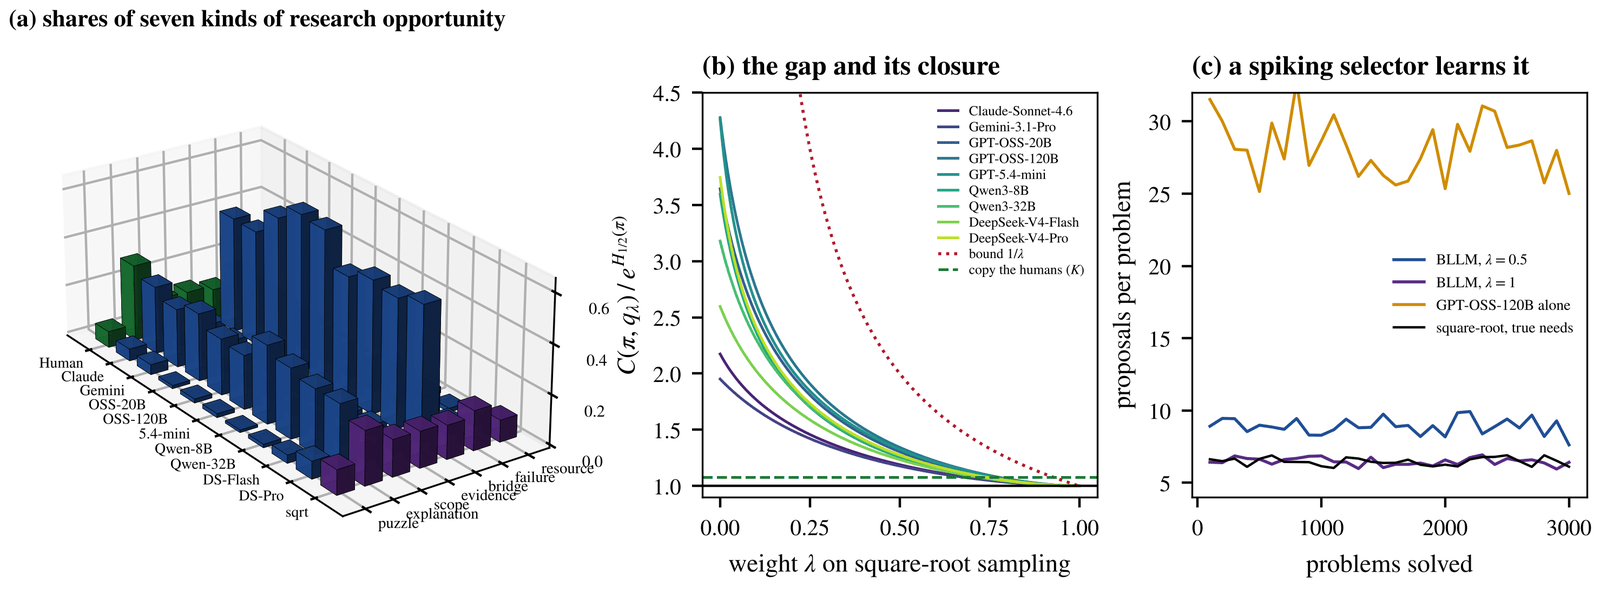
\includegraphics[width=0.98\textwidth]{figures/fig_gap}
\caption{The gap between human and LLM research ideas and its closure. (a) The shares of the seven kinds of research opportunity in the human papers and in the ideas of nine language models \cite{CZC26}, and square-root sampling of the human profile (``sqrt''); the models concentrate on bridge opportunities. (b) The cost of the mixture $q_{\lambda}$ of each model with square-root sampling, divided by the optimum $e^{H_{1/2}(\pi)}$, against the weight $\lambda$: every curve lies below the bound $1/\lambda$ of Theorem~\ref{thm:I}(iii), dotted, and falls below the cost of the human profile, dashed, at a weight between $0.68$ and $0.78$. (c) A stream of $3000$ problems with the opportunity profile of GPT-OSS-120B, mean proposals per problem over windows of $100$ problems and six seeds: the model alone pays $28.1$ against the $27.81$ of the law; a BLLM that draws half of its proposals from the spiking selector of Section~\ref{ssec:selector}, which learns only from the problems its checks close, pays $8.9$, the value $8.74$ of the law; with all proposals from the selector it pays $6.45$, the optimum $6.50$ of square-root sampling with the true needs.}
\label{fig:gap}
\end{figure*}

\subsection{Learning the need from the checks}

Square-root sampling needs $\pi$, and $\pi$ is not given. A BLLM learns it from its own record: every result its checks keep closes a problem with an idea of a known class, so after $n$ closed problems it has counts $c_{j}$ with $\sum_{j}c_{j}=n$, and it samples from the square root of the estimate $\hat\pi_{j}=(c_{j}+\alpha)/(n+K\alpha)$, with a prior count $\alpha>0$. The next proposition says how fast this closes the gap.

\begin{proposition}[Learning rate]\label{prop:learnrate}
Let the counts be multinomial with parameters $n$ and $\pi$, all $\pi_{j}>0$, and let $\hat r$ be square-root sampling of $\hat\pi$. Then
\begin{equation}\label{eq:learnrate}
\begin{gathered}\frac{\EE\,C(\pi,\hat r)}{e^{H_{1/2}(\pi)}}=1+\frac{\beta(\pi)}{4n}+o\Bigl(\frac1n\Bigr),\\ \beta(\pi)=\frac1S\sum_{j}\frac{1}{\sqrt{\pi_{j}}}-\frac{K}{S^{2}}\ \ge\ \frac{K(K-1)}{S^{2}} .\end{gathered}
\end{equation}
\end{proposition}

\begin{proof}
By Theorem~\ref{thm:I}(ii) the ratio is $1+\EE\,\chi^{2}(r\|\hat r)$. Write $\hat\pi=\pi+d$. The map $x\mapsto\chi^{2}(r\|\rho(x))$, with $\rho_{j}(x)=\sqrt{x_{j}}/\sum_{k}\sqrt{x_{k}}$, is smooth near $\pi$, vanishes at $\pi$ with its gradient, and its second-order part is computed from $\rho_{j}(\pi+d)-r_{j}=(u_{j}-r_{j}U)/S+O(|d|^{2})$, where $u_{j}=d_{j}/(2\sqrt{\pi_{j}})$ and $U=\sum_{j}u_{j}$:
\[
\begin{aligned}\chi^{2}(r\|\rho(\pi+d))&=\frac1S\sum_{j}\frac{(u_{j}-r_{j}U)^{2}}{\sqrt{\pi_{j}}}+O(|d|^{3})\\&=\frac1S\Bigl(\sum_{j}\frac{u_{j}^{2}}{\sqrt{\pi_{j}}}-\frac{U^{2}}{S}\Bigr)+O(|d|^{3}),\end{aligned}
\]
using $r_{j}/\sqrt{\pi_{j}}=1/S$ and $\sum_{j}r_{j}^{2}/\sqrt{\pi_{j}}=1/S$. The prior shifts the mean of $d$ by $O(1/n)$, and the covariance of $d$ is $(\mathrm{diag}(\pi)-\pi\pi^{\top})/n+O(n^{-2})$; so $\EE u_{j}^{2}=(1-\pi_{j})/(4n)+O(n^{-2})$ and $\EE U^{2}=\frac1{4n}\bigl(\sum_{j}(1-\pi_{j})-\sum_{j\ne k}\sqrt{\pi_{j}\pi_{k}}\bigr)+O(n^{-2})=\frac{K-S^{2}}{4n}+O(n^{-2})$. Substituting,
\[
\EE\,\chi^{2}=\frac1{4nS}\Bigl(\sum_{j}\frac{1-\pi_{j}}{\sqrt{\pi_{j}}}-\frac{K-S^{2}}{S}\Bigr)+o\Bigl(\frac1n\Bigr)=\frac{\beta(\pi)}{4n}+o\Bigl(\frac1n\Bigr),
\]
since $\sum_{j}(1-\pi_{j})/\sqrt{\pi_{j}}=\sum_{j}\pi_{j}^{-1/2}-S$. The remainder is $o(1/n)$: on the event $|d|\le\delta$ it is bounded by a constant times $\EE|d|^{3}=O(n^{-3/2})$, and off it $\chi^{2}(r\|\hat r)$ is at most a polynomial in $n$, because $\hat\pi_{j}\ge\alpha/(n+K\alpha)$, while the event has probability $e^{-cn}$ by Hoeffding's inequality \cite{Hoe63}. Finally $\sum_{j}\pi_{j}^{-1/2}\ge K^{2}/S$ by the Cauchy--Schwarz inequality, which gives the lower bound on $\beta$.
\end{proof}

For the human profile of opportunities $\beta=7.06$, so a BLLM that has closed $100$ problems pays $1.018$ times the optimum, and after $1000$ problems $1.0018$ times; simulation gives $1.019$ and $1.0018$, and at $n=20$, where the expansion is not yet accurate, $1.083$. The correction is of order $K^{2}/n$ and does not depend on the proposer at all: the gap of a language model is a fixed multiple, the gap of a learning selector disappears like $1/n$.

\subsection{A spiking selector}\label{ssec:selector}

The selector that the BLLM package uses is a circuit of spiking neurons, chosen because it computes square-root sampling exactly with the elements and the learning rule that nervous systems use for the selection of actions \cite{RPG99,SDM97,FG16} and that neuromorphic hardware implements \cite{Mea90,Maa97,DSL18}. There is one leaky integrate-and-fire neuron for each class, or for each agent; the membrane potential $u_{k}$ of neuron $k$ relaxes with time constant $\tau$ to its synaptic drive $w_{k}$, and the neuron fires in continuous time with the escape rate $\rho_{0}e^{(u_{k}-\vartheta)/\delta}$ \cite{GKN14}. The first neuron to fire chooses. When a check keeps a result produced by class $k$, a reward, the third factor of a three-factor rule \cite{FG16}, potentiates that synapse,
\begin{equation}\label{eq:spikereward}
w_{k}\leftarrow w_{k}+\frac\delta2\log\frac{c_{k}+1+\alpha}{c_{k}+\alpha},\qquad c_{k}\leftarrow c_{k}+1,
\end{equation}
and synaptic scaling \cite{TLD98} then shifts all weights by a common amount that keeps the total rate equal to $\rho_{0}$.

\begin{proposition}[The selector samples the square root of what it has learned]\label{prop:spiking}
Once the membranes have relaxed, the neuron that fires first is $k$ with probability $e^{w_{k}/\delta}/\sum_{l}e^{w_{l}/\delta}$, and after the rewards \eqref{eq:spikereward} this probability is $\sqrt{c_{k}+\alpha}/\sum_{l}\sqrt{c_{l}+\alpha}$, square-root sampling of the estimated need $\hat\pi$.
\end{proposition}

\begin{proof}
With relaxed membranes, $u_{k}=w_{k}$ and the neurons fire as independent Poisson processes of rates $\lambda_{k}=\rho_{0}e^{(w_{k}-\vartheta)/\delta}$. The first spike of neuron $k$ is exponential with rate $\lambda_{k}$, and the least of independent exponential times is the $k$-th with probability $\lambda_{k}/\sum_{l}\lambda_{l}$. The increments \eqref{eq:spikereward} telescope, so after $c_{k}$ rewards $w_{k}=w_{k}(0)+\frac\delta2\log\frac{c_{k}+\alpha}{\alpha}$, and the scaling adds the same constant to every $w_{l}$, which cancels in the ratio. With equal initial weights, $e^{w_{k}/\delta}$ is proportional to $\sqrt{c_{k}+\alpha}$.
\end{proof}

In the package the membranes are integrated with a step $\mathrm{d}t$ and the race opens after five time constants, so the probabilities hold up to terms of order $\rho_{0}\,\mathrm{d}t$ and $e^{-5}$; over $40{,}000$ races they agree with $\sqrt{c_{k}+\alpha}/\sum_{l}\sqrt{c_{l}+\alpha}$ to within $0.007$. Combined with Proposition~\ref{prop:learnrate}, the circuit closes the gap at the rate $\beta/(4n)$, and it does so with nothing a nervous system lacks: a race to threshold, a reward that potentiates the winner, and a homeostatic scaling of the total rate. Figure~\ref{fig:gap}(c) shows it on the profile of GPT-OSS-120B. The selector never decides a result; it only chooses which class, or which agent, proposes next, and every proposal meets the checks, so the soundness of Theorems~\ref{thm:A} to~\ref{thm:H} is untouched and the gap law is a statement about cost alone.

\subsection{What the gap law says, and what it does not}

The law is exact for its model: independent proposals, a need that is a distribution over classes, and a proposer that keeps drawing until the class is right. Reaching the right class is necessary for reaching the right idea, not sufficient, and within a class a proposer may still fail; that part is priced by the checks, and the two costs multiply. The need is taken from the human papers, which is the only meaning the measurement of \cite{CZC26} gives to the right class; if the human profile is itself biased, square-root sampling of a better need is better still, and the law applies unchanged. What the law gives is a closed form for the cost of the gap that was measured, the proof that this cost is a chi-squared divergence from square-root sampling, a universal bound for its closure, and a circuit that reaches the optimum by learning from its checks at the rate $\beta/(4n)$. It does not make a language model think like a person. It makes a system that contains a language model search for ideas, at the level of the classes measured, with fewer proposals than either the model or a proposer with human taste.

\section{Branching takeoff}\label{sec:branching}

\subsection{The tree of improvements}

A self-improving system need not move along a chain. Each kept improvement may spawn several candidates for the next, and the improvements form a tree (Fig.~\ref{fig:branchtree}). The model is a Galton--Watson process with checks.

\begin{definition}[Checked branching process]\label{def:branching}
Generation $0$ is one kept correct system. Each kept correct improvement of generation $k-1$ spawns an independent copy of a random number $\xi\ge0$ of candidates, with $\EE\,\xi=\mu$ and $\PR(\xi\ge1)>0$. Each candidate is correct with probability $\gamma\in(0,1)$, independently. The check of generation $k$ keeps a correct candidate with probability $1-\eta$ and an incorrect one with probability $\delta_{k}\in(0,1]$. Kept incorrect candidates are quarantined: they spawn nothing. Let $Z_{k}$ be the number of kept correct improvements of generation $k$, $F_{k}$ the number of kept incorrect ones, $F=\sum_{k\ge1}F_{k}$, and $m=\mu\gamma(1-\eta)$.
\end{definition}

The number $N$ of kept correct offspring of one kept correct improvement is obtained from $\xi$ by keeping each candidate independently with probability $\gamma(1-\eta)$, so $(Z_{k})$ is a Galton--Watson process with offspring law $N$ and mean $\EE N=m$. If $\xi$ is Poisson with mean $\mu$, then $N$ is Poisson with mean $m$. The quarantine assumption is needed only for the formula for $\EE F$; without it $F$ is larger, so the statements that force $F=\infty$ hold a fortiori.

\begin{figure*}[t]
\centering
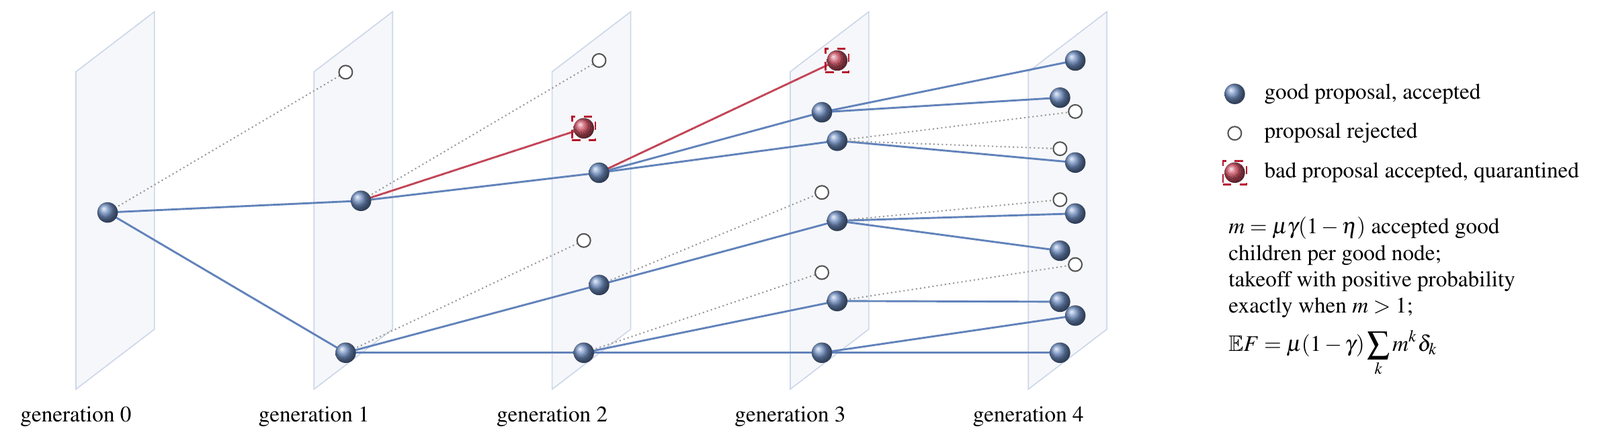
\includegraphics[width=0.92\textwidth]{figures/fig_branchtree}
\caption{A checked branching process, Definition~\ref{def:branching}, over four generations drawn as sheets. Blue nodes are kept correct improvements, which spawn the next generation; grey nodes are rejected candidates; red nodes are incorrect candidates that the check kept, which are quarantined. The kept correct improvements grow like $m^{k}$ in mean, and the expected number of kept errors is $\mu(1-\gamma)\sum_{k}m^{k-1}\delta_{k}$ (Theorem~\ref{thm:F}).}
\label{fig:branchtree}
\end{figure*}

\subsection{Takeoff}

The process \emph{takes off} if $Z_{k}>0$ for every $k$. Let $f(z)=\EE\,z^{N}$ and $q=\PR(\text{takeoff})$.

\begin{proposition}[Takeoff threshold]\label{prop:takeoff}
Assume $\PR(N=1)<1$. Then $q>0$ if and only if $m>1$, and $1-q$ is the least root of $f(z)=z$ in $[0,1]$. If moreover $\EE N^{2}<\infty$ and $m>1$, then
\[
\frac{2(m-1)}{f''(1)}\ \le\ q\ \le\ \frac{2(m-1)}{f''(1-q)} .
\]
For Poisson offspring, $f''(1)=m^{2}$, $f''(1-q)=m^{2}(1-q)$ and, for $1<m\le2$, $\bigl|q-2(m-1)/m^{2}\bigr|\le4e^{4}(m-1)^{2}$.
\end{proposition}

\begin{proof}
The first two claims are the classical extinction theorem \cite{AN72,WG75}; Appendix~\ref{app:gw} recalls the proof. For the bounds, Taylor's formula at $1$ with $f(1)=1$ and $f'(1)=m$ gives $f(1-q)=1-mq+\frac12f''(\xi)q^{2}$ for some $\xi\in(1-q,1)$. Since $f(1-q)=1-q$, this is $(m-1)q=\frac12f''(\xi)q^{2}$, so $q=2(m-1)/f''(\xi)$; and $f''$ is increasing on $[0,1]$, being a power series with nonnegative coefficients, so $f''(1-q)\le f''(\xi)\le f''(1)$. For Poisson offspring $f(z)=e^{m(z-1)}$, $f''(z)=m^{2}e^{m(z-1)}$, and $e^{-mq}=1-q$ at the fixed point. The two bounds then differ by $\frac{2(m-1)}{m^{2}}\cdot\frac{q}{1-q}$. Extinction has probability at least $\PR(N=0)=e^{-m}\ge e^{-2}$, so $1-q\ge e^{-2}$ and $q\le2e^{2}(m-1)$; the difference is at most $2(m-1)e^{2}\cdot2e^{2}(m-1)$.
\end{proof}

Near the threshold the probability of takeoff is linear in $m-1$, with slope $2/f''(1)$, which tends to $2/\sigma^{2}$ at criticality, $\sigma^{2}$ the variance of the offspring law there; Table~\ref{tab:gw} gives the numbers for Poisson offspring and Fig.~\ref{fig:branching}(a) the curves. A takeoff is never certain: for $m\le2$ it fails with probability at least $e^{-2}$, and it is a matter of luck in its first generations.

\begin{table}[b]
\caption{Probability $q$ of takeoff for Poisson offspring of mean $m$, with the two bounds of Proposition~\ref{prop:takeoff}.}
\label{tab:gw}
\centering
\small
\begin{tabular}{@{}c c c c@{}}
\toprule
$m$ & $2(m-1)/m^{2}$ & $q$ & $2(m-1)/(m^{2}(1-q))$ \\
\midrule
$1.02$ & $0.0385$ & $0.0390$ & $0.0400$ \\
$1.05$ & $0.0907$ & $0.0937$ & $0.1001$ \\
$1.10$ & $0.1653$ & $0.1761$ & $0.2006$ \\
$1.20$ & $0.2778$ & $0.3137$ & $0.4048$ \\
$1.50$ & $0.4444$ & $0.5828$ & $1.0653$ \\
$2.00$ & $0.5000$ & $0.7968$ & $2.4608$ \\
\bottomrule
\end{tabular}
\end{table}

\subsection{Errors in a takeoff}

\begin{proof}[Proof of Theorem~\ref{thm:F}]
\emph{Threshold.} This is Proposition~\ref{prop:takeoff}.

\emph{Expected errors.} Let $\mathcal F_{k}$ be the information of generations $0,\dots,k$. Given $\mathcal F_{k-1}$, the $Z_{k-1}$ kept correct improvements spawn on average $\mu Z_{k-1}$ candidates, each incorrect and kept with probability $(1-\gamma)\delta_{k}$, so $\EE[F_{k}\mid\mathcal F_{k-1}]=\mu(1-\gamma)\delta_{k}Z_{k-1}$. With $\EE Z_{k-1}=m^{k-1}$ and monotone convergence, $\EE F=\mu(1-\gamma)\sum_{k\ge1}m^{k-1}\delta_{k}$. If the series converges, $F<\infty$ almost surely.

\emph{Divergence.} Let $m>1$, $\EE\,\xi\log\xi<\infty$ and $\sum m^{k-1}\delta_{k}=\infty$. Since $N\le\xi$, also $\EE N\log N<\infty$, and the Kesten--Stigum theorem \cite{KS66,AN72} gives $Z_{k}/m^{k}\to W$ almost surely with $W>0$ almost surely on takeoff. Let $B_{k}=\{F_{k}\ge1\}\in\mathcal F_{k}$ and $u_{k}=(1-\gamma)\delta_{k}$. Given $\mathcal F_{k-1}$ the parents act independently, and one parent with $\xi$ candidates keeps no incorrect one with probability $\EE(1-u_{k})^{\xi}\le1-u_{k}\PR(\xi\ge1)$, because $1-(1-u)^{j}\ge u$ for $j\ge1$. With $c_{0}=\PR(\xi\ge1)>0$,
\[
\begin{aligned}
\PR(B_{k}\mid\mathcal F_{k-1})&\ \ge\ 1-(1-c_{0}u_{k})^{Z_{k-1}}\ \ge\ 1-e^{-c_{0}u_{k}Z_{k-1}}\\
&\ \ge\ \tfrac12\min(c_{0}u_{k}Z_{k-1},1),
\end{aligned}
\]
the last step by $1-e^{-x}\ge\frac12\min(x,1)$. On takeoff, $Z_{k-1}\ge\frac12Wm^{k-1}$ for all large $k$, so up to finitely many terms
\[
\sum_{k}\PR(B_{k}\mid\mathcal F_{k-1})\ge\frac12\sum_{k}\min\Bigl(\frac{c_{0}(1-\gamma)W}{2}\,m^{k-1}\delta_{k},\,1\Bigr).
\]
 The right side diverges, since $\sum m^{k-1}\delta_{k}$ diverges and a series $\sum\min(cx_{k},1)$ with $c>0$, $x_{k}\ge0$ converges only if $\sum x_{k}$ does. L\'evy's conditional Borel--Cantelli lemma \cite{Dur19} states that $\{B_{k}\text{ infinitely often}\}$ and $\{\sum_{k}\PR(B_{k}\mid\mathcal F_{k-1})=\infty\}$ agree up to a null set (Appendix~\ref{app:levy}). So $F=\infty$ almost surely on takeoff.

\emph{Exponential checks.} With $\delta_{k}=\eps^{r_{k}}$ and $r_{k}=\lceil k\log(2m)/L\rceil$, $r_{k}L\ge k\log(2m)$, so $m^{k}\eps^{r_{k}}\le2^{-k}$ and $\sum m^{k-1}\delta_{k}\le\frac1m\sum2^{-k}<\infty$. Conversely, if $\sum m^{k-1}\eps^{r_{k}}<\infty$, its terms tend to $0$, so $r_{k}L-(k-1)\log m\to\infty$, hence $r_{k}L\ge k\log m$ for all large $k$. A constant $\delta_{k}=\delta>0$ gives $\sum m^{k-1}\delta=\infty$ for $m\ge1$.
\end{proof}

\begin{corollary}[The entropy tax of a takeoff]\label{cor:branchtax}
In a sound takeoff with exponential checks and $m>1$, every kept correct improvement of generation $k$ has been checked by at least $k\log m/L=\log(\EE Z_{k})/L$ runs, for all large $k$.
\end{corollary}

The tax is the logarithm of the size of the population, divided by $L$, exactly as for $n$ candidates of equal cost in Corollary~\ref{cor:uniform}: a growing population of improvements can stay sound only if each new improvement is checked harder than the last by a fixed number of runs per generation, and a fixed false acceptance rate, however small, lets errors multiply with the population (Fig.~\ref{fig:branching}(b)).

\begin{figure*}[t]
\centering
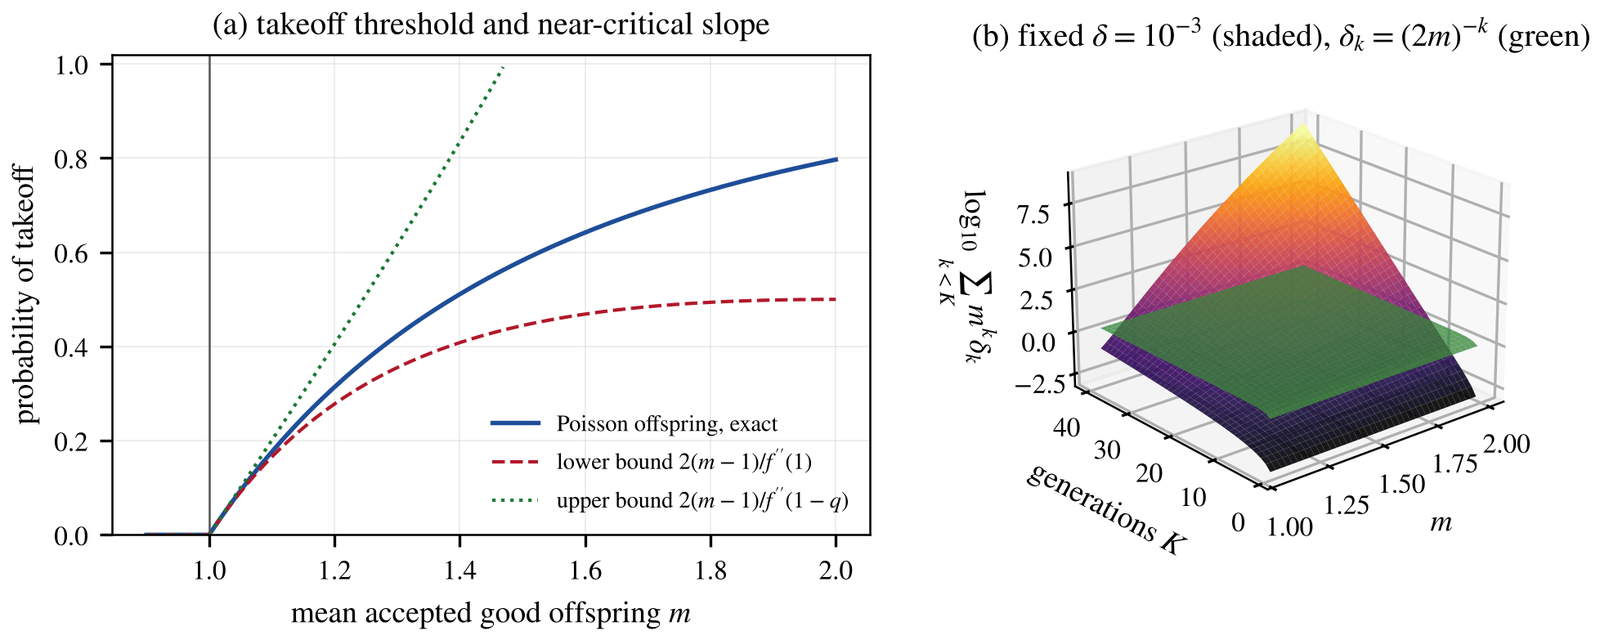
\includegraphics[width=0.98\textwidth]{figures/fig_branching}
\caption{Theorem~\ref{thm:F}. (a) The probability of takeoff for Poisson offspring as a function of the mean $m$ of kept correct offspring, with the two bounds of Proposition~\ref{prop:takeoff}; the threshold is $m=1$ and the slope there is $2$. (b) The expected number of kept errors in the first $K$ generations, $\log_{10}\sum_{k<K}m^{k}\delta_{k}$, for a fixed rate $\delta=10^{-3}$ (shaded surface), which grows without bound, and for the amplified rate $\delta_{k}=(2m)^{-k}$ (green), which stays below $\log_{10}2$.}
\label{fig:branching}
\end{figure*}

\section{Towers of verified layers}\label{sec:towers}

A BLLM can act on another BLLM. The proposer of Section~\ref{sec:network} that builds a graph is one engine; an engine that chooses among strategies of that proposer and keeps the ones that build faster is a second, standing on the first; an engine that runs several copies of the second and keeps the better half after each round is a third. We call a stack of $n$ such engines a \emph{tower of depth $n$}, write it $B^{n}$, and ask what depth costs. The answer is a corollary of the entropy law, and it bounds what any implementation of depth can gain.

\subsection{The model}

Let a tower have layers $0,\dots,n-1$. Layer $k$ passes an object up only after it has been certified, and a false acceptance at layer $k$ contaminates every layer above it, since the layers above build on what it passed. So the layers share one budget: the false acceptance probabilities $\beta_{k}$ of the $n$ certifications satisfy $\sum_{k<n}\beta_{k}\le\theta$, and the certification cost of the tower is $\sum_{k<n}\log(1/\beta_{k})$ nats of soundness. A layer certified by $r_{k}$ independent runs of a check of soundness $\eps$ has $\beta_{k}=\eps^{r_{k}}$ and costs $r_{k}$ runs. The search cost $S_{n}$ of the tower, the work its layers do before anything is certified, is left arbitrary except for a lower bound $B$ that every stage pays.

The same model covers a \emph{mesh}, in which the layers read and write one shared library and the connections between them are strengthened when they are used. Every object enters the shared library only after the independent check of Section~\ref{ssec:construct}, so a false acceptance still contaminates every user of the library, and the count of certified passes, not the wiring, is what enters the bounds below.

\subsection{What depth costs}

\begin{theorem}[Tower law]\label{thm:tower}
Let $0<\theta\le1$ and $n\ge1$.
\begin{enumerate}[label=\textup{(\roman*)},leftmargin=2.2em,itemsep=1pt]
\item If $\beta_{k}>0$ and $\sum_{k<n}\beta_{k}\le\theta$, then $\sum_{k<n}\log(1/\beta_{k})\ge n\log(n/\theta)$; with exponential checks of soundness $\eps$, a tower needs at least $n\log(n/\theta)/\log(1/\eps)$ runs in all.
\item Adding a layer raises the bound of \textup{(i)} by at least $\log((n+1)/\theta)$, and these increments tend to infinity.
\item If every stage costs at least $B$ to search and the certification of a depth-$n$ tower costs at least $c\,n\log(n/\theta)$ with $c>0$, then for every $T_{1}$ there is a depth $N$ such that every tower of depth $n\ge N$ costs more than $T_{1}$; in particular, past a finite depth every tower costs more than the tower of depth one.
\item Along an infinite tower whose budgets $\beta_{k}>0$ are summable, the certification cost $\log(1/\beta_{k})$ of a single stage tends to infinity.
\end{enumerate}
\end{theorem}

\begin{proof}
(i) is the lower bound of Theorem~\ref{thm:A} for $n$ candidates of unit cost: with $a_{k}=1$ the entropy of the profile is $\log n$, and the bound reads $\sum_{k}r_{k}\ge(n/L)(\log n+\log\frac1\theta)$; in nats of soundness this is $\sum_{k}\log(1/\beta_{k})\ge n\log(n/\theta)$. (ii) With $f(n)=n\log(n/\theta)$, $f(n+1)-f(n)=\log((n+1)/\theta)+n\log((n+1)/n)\ge\log((n+1)/\theta)$, and $\log((n+1)/\theta)\to\infty$. (iii) For $n\ge3$ and $\theta\le1$ we have $n/\theta\ge3>e$, so $\log(n/\theta)\ge1$ and the cost is at least $B+c\,n$, which exceeds $T_{1}$ as soon as $n>(T_{1}-B)/c$. (iv) A summable sequence of positive terms tends to $0$, so $1/\beta_{k}\to\infty$.
\end{proof}

The six statements are proved in Lean in the file \texttt{Tower}, listed in Table~\ref{tab:lean2}.

The theorem is a ceiling, not a recipe. Depth is worth paying for only while it lowers the search cost $S_{n}$ by more than the increment of (ii), and (iii) says that this stops at a finite depth whatever the search does. A tower that seems to gain without limit from depth is either uncertified somewhere or spending its soundness budget faster than it says. Section~\ref{ssec:towerbench} measures $S_{n}$ for $n=1,2,3$, ladder and mesh, at equal budgets of exact checks.

\begin{remark}[Postnikov towers]\label{rem:postnikov}
A Postnikov tower of a connected CW complex $X$ is a sequence of fibrations $\cdots\to X_{n}\to X_{n-1}\to\cdots\to X_{1}$ with maps $X\to X_{n}$ that are isomorphisms on $\pi_{k}$ for $k\le n$, where $\pi_{k}(X_{n})=0$ for $k>n$ and each fibre of $X_{n}\to X_{n-1}$ is an Eilenberg--MacLane space $K(\pi_{n}(X),n)$ \cite[Section~4.3]{Hat02}. We use the picture in one precise sense. Stage $n$ of the tower is the engine cut at depth $n$, and passing from stage $n-1$ to stage $n$ adds exactly one layer, whose cost is the increment of Theorem~\ref{thm:tower}(ii); that increment is the only part of the picture the paper uses, and it is proved. That the passage is a fibration, that it has a fibre with one nonzero invariant, or that the stages are glued by $k$-invariants has no counterpart in the engine, and we do not claim one.
\end{remark}

\section{Anaxia: the engine}\label{sec:network}

The theorems of the preceding sections price the checking of candidates and bound the number of proposals any proposer needs. They say nothing about where candidates come from. This section describes Anaxia, the engine we built to supply them, in the order in which a candidate meets its parts. In the crossing network, known constructions are typed nodes, new candidates are crosses of old ones, every cross is checked and then refuted if possible, and every outcome is written to a memory that steers the next cross (Fig.~\ref{fig:channel}). Construction mode writes down a new object, a graph, together with the argument for what it forces, and has it checked again by code that shares nothing with the search. The tower of Section~\ref{sec:towers} stacks construction mode into layers. A registry records what each part takes from earlier systems, and the whole is released as one package.

\begin{figure*}[t]
\centering
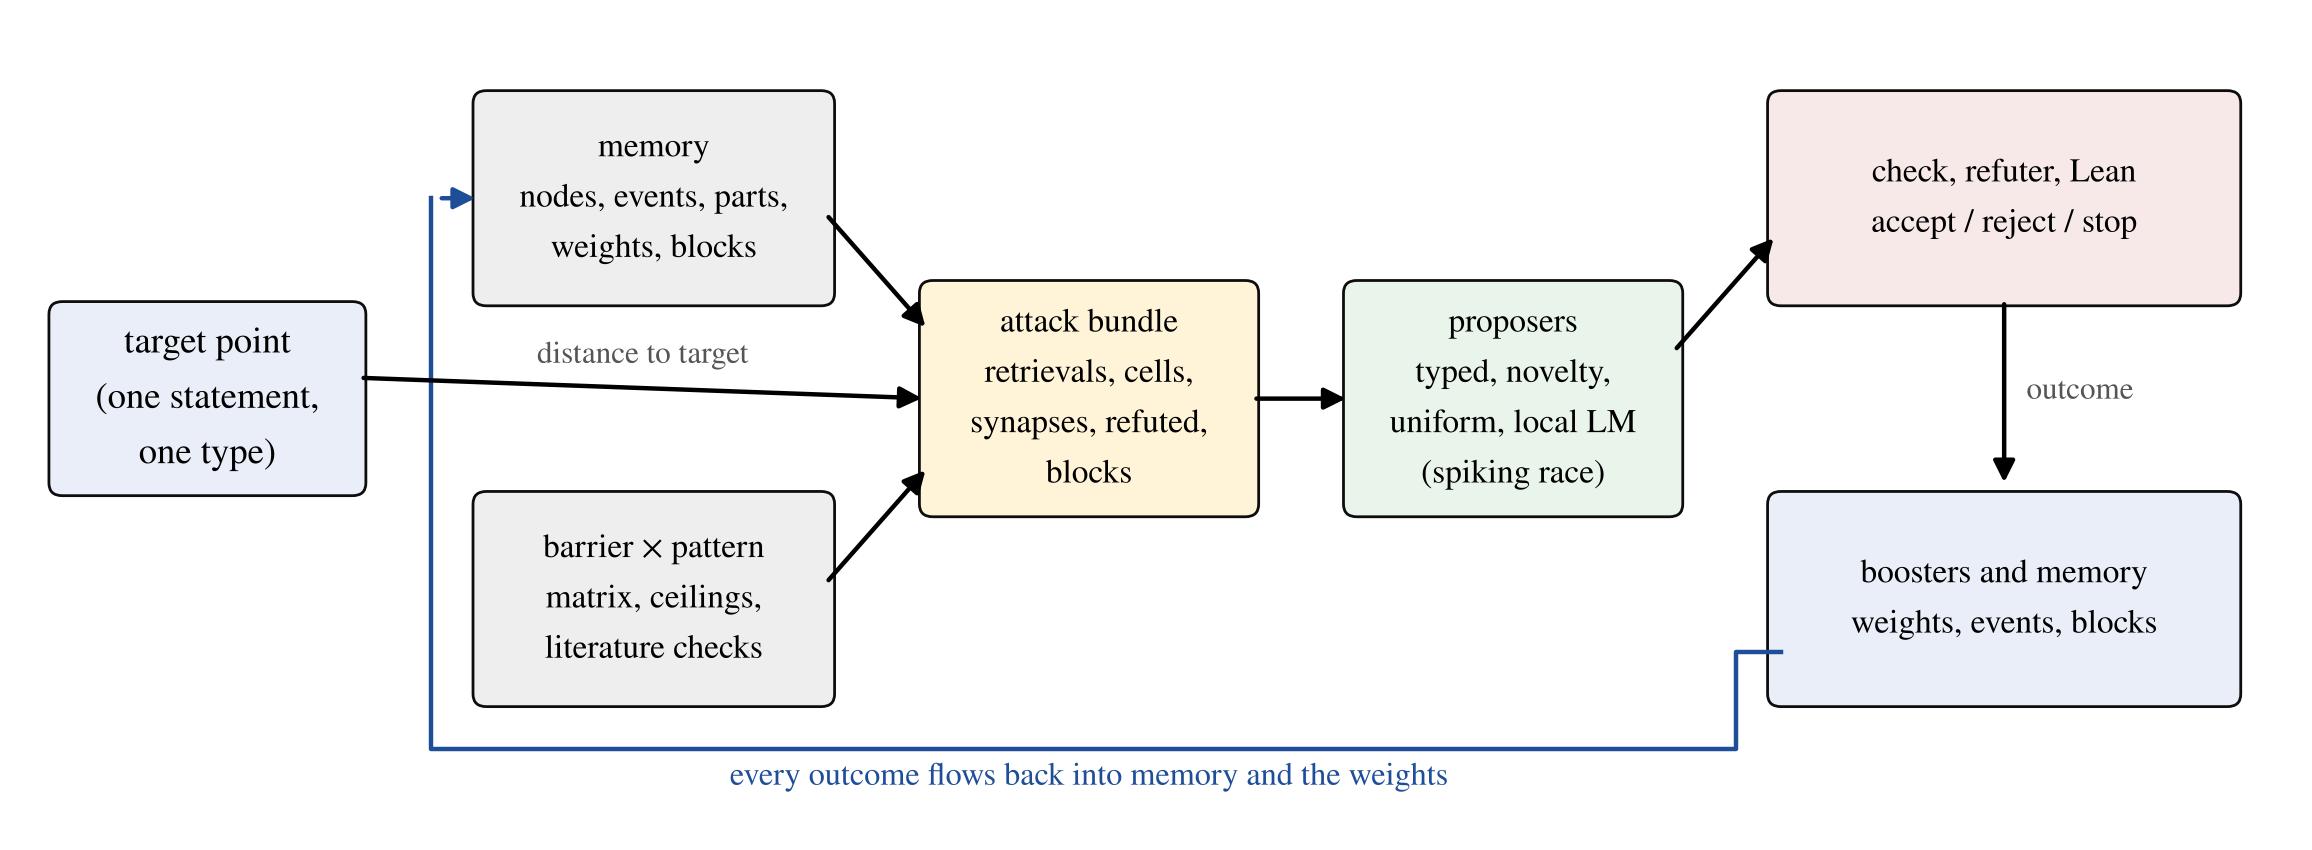
\includegraphics[width=0.98\textwidth]{figures/fig_channel}
\Description{Diagram of one round of the attack loop: a target type, the distance of each composite to it, and the attack bundle fed back to the generator.}
\caption{One round of the attack loop. The target point of a benchmark fixes a type; every composite gets a distance to that type. The attack bundle collects, for each candidate cross, the most similar past attempts in memory, the cells of the barrier and pattern matrix that touch its parts, the weights of its synapses, the refuted offspring of its parts and the blocks recorded on its problem. The proposers draw from the weighted candidates; the check, the refuter and, for a new statement, Lean decide the outcome, which updates the boosters and the memory before the next round.}
\label{fig:channel}
\end{figure*}

\subsection{Constructions as typed nodes}

A \emph{construction} $c$ is a record of three items: $\mathrm{gives}(c)$, the type of the object it produces; $\mathrm{needs}(c)$, the list of types it consumes; and $\mathrm{source}(c)$, the published result or computation it comes from. The single-link law of $\mathrm{SU}(2)$ gives a link law and needs nothing; Dobrushin's uniqueness criterion \cite{Dob68} gives a range of couplings and needs a dependency graph and an influence bound; Shioda's inductive structure \cite{Shi79} gives a splitting of a Fermat character and needs a character table. If $\mathrm{gives}(b)\in\mathrm{needs}(a)$, the \emph{cross} $a\leftarrow b$ is the construction with the first such input of $a$ filled by $b$; its parts are the union of the parts of $a$ and $b$. A composite with no unfilled input is \emph{closed}, and only closed composites are checked. Typing removes ill-formed candidates before any check: on the Yang--Mills library, crossing without regard to types wastes $45.4$ of $48$ crosses per run on ill-typed pairs (Table~\ref{tab:boosters}).

The library of a benchmark is the set of its constructions. Five libraries are used: Yang--Mills ($38$ nodes), Hodge ($28$), the standard conjecture of Lefschetz type ($17$), Chowla's conjecture ($20$) and Erd\H{o}s problem 1183 ($13$). Of these $116$ nodes, $54$ are literature constructions written out with their key lemma and the barrier at which they stop, for instance the Kotecký--Preiss criterion, the Brydges--Yau and Gaw\c{e}dzki--Kupiainen block-spin flows, Holley--Stroock and Stroock--Zegarlinski for Yang--Mills; van Geemen, Ribet, Kuga--Satake, Varesco and Charles--Markman for Hodge; Friedlander--Iwaniec, Heath-Brown, Green--Tao and Matomäki--Radziwi{\l}{\l}--Tao for Chowla.\footnote{The list is the file \texttt{knowledge.json} of the package. Each entry carries the problem it addresses, its typed inputs and output, the published source, the lemma that does the work, and a verdict: \emph{known} when the construction proves a published statement, \emph{stops} when it is known to fail at the benchmark's blocking step, with the reason. A literature node is never counted as progress: a composite that reaches a known statement is accepted as known and rewarded at a quarter of the rate of a new one, and a composite through a node marked \emph{stops} is stopped with that node's reason.}

\subsection{Checks and the refuter}

The check of a closed composite is a program attached to its output type. It returns \emph{accepted} with a measurement, \emph{rejected} with the measurement that failed, or \emph{stopped} when no checkable form of the composite exists. On Yang--Mills the check of a Dobrushin composite counts the active partners of a link in the dependency graph the composite names and computes the range $\beta_{W}<1/(\text{partners}\cdot\frac14)$ from the influence bound; on the Fermat fourfolds it enumerates the zero-sum splittings of the characters in an orbit; on Erd\H{o}s problem 1183 it computes the largest monochromatic sublattice by the search of Lemma~\ref{lem:levelposet}. An accepted composite then meets the \emph{refuter}, which breaks it if its range is dominated by one already known, if it reproduces an accepted statement without gain, or if it rests on an unrefereed claim. Only composites that pass both count as survivors. A survivor whose statement is new is formalised in Lean before it is reported; none of the five pass lines has such a survivor.

\subsection{Boosters}

Every ordered pair of library heads carries a synapse with weight $w$, initially $1$. When a cross fires and its offspring survives, its synapse rises by $\eta$, and the synapses that built its parents rise by $\eta\gamma^{k}$ at distance $k\le4$; a rejected or refuted offspring lowers its synapse by $\eta/2$, to no less than $0.05$. After each generation the weights leaving each node are rescaled to mean one, and a share $\eps$ of the crosses is drawn uniformly. We use $\eta=1$, $\gamma=\frac12$ and $\eps=0.2$. This is a Hebbian rule with path credit, and Section~\ref{ssec:boosters} measures what it adds.

\subsection{Memory}

The memory is one SQLite store shared by every proposer and every round. It holds the nodes, one event per checked composite (its parts, outcome, measurement, reason, synapse weight, round and proposer), an index from parts to events, the synapse weights, the blocks (for each problem and step, the assumption that stopped it and the source of the stopping composite), the literature checks, and a log of every retrieval. Two uses follow.
\begin{enumerate}[label=(\roman*),leftmargin=1.8em,itemsep=1pt]
\item \emph{Decided composites are skipped.} A composite whose parts already have an event is not checked again; this is what removes the repeated checks of Fig.~\ref{fig:memory}(b).
\item \emph{Retrieval steers the draw.} For a candidate with part set $Q$, the $k=5$ past events with the largest score $J(Q,S)\,w$ are retrieved, where $S$ is the part set of the event, $J$ the Jaccard similarity and $w$ the synapse weight at the time. The candidate's weight is multiplied by
\begin{equation}\label{eq:memprior}
\pi_{\mathrm{mem}}(Q)=\min\Bigl(3,\ \max\Bigl(\tfrac14,\ 1+\sum_{\text{survivors}}J-\tfrac12\sum_{\text{others}}J\Bigr)\Bigr),
\end{equation}
which raises it near past survivors and lowers it near failures.
\end{enumerate}
The store of a five-round study over all five libraries holds $42$ events, $11$ blocks and $26$ weights in $156$ kilobytes, so the memory is small and the check, not the bookkeeping, is the cost.

\subsection{Target points and the attack channel}

A \emph{target point} is one statement whose proof would cross the wall of a benchmark, together with its type. For Erd\H{o}s problem 1183 it is a family of colourings of $2^{[n]}$ whose monochromatic sublattices have at most $n/2+C$ members for every $n$; for Yang--Mills, an effective action at one coupling $\beta_{W}>\frac13$ whose blocked measure satisfies a Dobrushin-type condition uniformly in the spacing; for Hodge, the algebraicity of the class of the character $(1,16,26,31,36)$ of level $55$ on the Fermat fourfold of degree $110$; for Chowla, local $U^{2}$ uniformity of the Liouville function on almost all intervals of length $\exp((\log X)^{2/5-\delta})$, one step below the scale of \cite{Pil26}; for the standard conjecture, an algebraic inverse of $L$ on $H^{2}$ of one threefold of general type with $h^{2,0}>0$. A backward search over the library gives every type a distance: $0$ for the target type, and $1+d$ for each input of a construction whose output is at distance $d$. A candidate's weight is multiplied by $e^{-d}$, where $d$ is the distance of its output, so the forward search by crossing and the backward search from the target meet at the composites of distance $0$ and $1$.

The \emph{attack channel} is the single pipeline that hands everything the engine holds to the proposers. For each candidate it builds a bundle: the retrievals, the cells of the barrier and pattern matrix that touch its parts (Section~\ref{ssec:matrix}), the weights of its synapses, the refuted offspring among the retrievals, and the blocks of its problem. The bundle multiplies the weight by
\begin{equation}\label{eq:channelprior}
\pi_{\mathrm{ch}}=\min\Bigl(5,\ \max\Bigl(0.05,\ 2^{-n_{\mathrm{fail}}}\,(\tfrac32)^{n_{\mathrm{part}}}\bigl(1+\textstyle\sum_{\text{survivors}}J\bigr)\Bigr)\Bigr),
\end{equation}
where $n_{\mathrm{fail}}$ and $n_{\mathrm{part}}$ count the cells of the bundle whose recorded outcome is a failure or a partial result. Every bundle that flows is written to the memory, so that a run with the channel can be compared with one without.

\subsection{Proposers and agents}

Four proposers share the weighted candidates: \emph{typed} draws in proportion to the weight; \emph{novelty} takes the candidate least similar to anything in memory; \emph{uniform} draws uniformly; and \emph{local model} shows the eight heaviest candidates and the retrieved notes to a local language model with $5\times10^{8}$ parameters \cite{Qwe24} and takes the one it names. Which proposer moves is decided by the spiking selector of Proposition~\ref{prop:spiking}, rewarded on survivors, so that the committee samples the square root of each proposer's record of success, the optimum of Theorem~\ref{thm:I}.

An \emph{agent} holds one target point, its own library, its own synapse weights and its slice of the shared memory. Each step it attacks its library through the channel. When a step adds no survivor it runs a sub-attack whose target is the nearest open input type of its target point, a lemma at distance one. Agents trade through the memory: a result passes from one agent to another only where one benchmark is an input of another, which among the five happens once, since the standard conjecture for $X$ is a case of the Hodge conjecture on $X\times X$. Both are package code, not language-model agents: an agent is an object with a library, weights and a memory slice, and its step is a call of the attack.

\subsection{Construction mode}\label{ssec:construct}

The crossing network only combines results that someone has already proved. Construction mode builds an object that no one has written down, on problems where the object is finite: planar graphs whose proper $3$-colourings are constrained at a few \emph{contact} vertices on one face. Such a graph is a \emph{gadget}; it is a not-all-equal forcer if no proper $3$-colouring gives its three contacts one colour, and its \emph{profile} is the list of distances between its contacts. Gadgets of this kind are the building blocks of the refutation of Steinberg's conjecture by Cohen-Addad, Hebdige, Kr\'al', Li and Salgado, a planar graph with no cycles of length $4$ or $5$ that is not $3$-colourable \cite{CHK17}, and of every attempt on Erd\H{o}s's question whether a planar graph with no cycles of length $4$, $5$ or $6$ is $3$-colourable.

The builder grows a gadget together with its forcing argument. It assumes that the contacts share a colour $\gamma$ and applies four moves: \emph{attach} a new vertex next to a $\gamma$ vertex, which is then not $\gamma$; \emph{link} two vertices that are not $\gamma$, whose colours then differ; \emph{derive} a new vertex next to two vertices whose colours are known to differ, which is then $\gamma$; and \emph{close} with an edge or a triangle that leaves no colouring. A library gadget may also be inserted as a lemma, with its contacts sent to vertices of the graph. Between moves the builder propagates the forced colours to a fixed point and adds structure only when nothing more follows. Every move passes a cascade of tests before it is kept: no cycle of a forbidden length through a new edge, contact distances at least those of the profile, and planarity with the contacts on one face; only then does an exact satisfiability check decide whether the contacts can still share a colour. When they cannot, the graph is minimised and offered to the gate.

The \emph{gate} is code that shares nothing with the builder: planarity by the left--right algorithm of \texttt{networkx}, every cycle of forbidden length by depth-first search, the contact distances by breadth-first search, and the absence of a colouring with equal contacts by plain backtracking with no satisfiability solver. A gadget counts only when the gate accepts it, and the whole counterexample assembled from a gadget is checked again by three satisfiability solvers, CaDiCaL, Glucose and MiniSat. A second search writes the forcing condition as an exists-forall problem: a satisfiability instance over the edge variables, with planarity built in by a $2$-page book embedding and every $3$-colouring that defeats a candidate turned into a clause that every forcer satisfies. The cost of every run is counted in exact satisfiability checks, so that different searches can be compared at the same budget.

\subsection{The tower of builders}\label{ssec:tower}

The tower $B^{n}$ of Section~\ref{sec:towers} is built over construction mode. Layer~$1$ is the builder with one fixed strategy: the order in which it tries the four moves, how much noise it adds to that order, and how often it tries a lemma. Layer~$2$ acts on layer~$1$: it keeps a population of strategies, runs each for a slice of checks, keeps the better half by gadgets found per check and refills the population with mutations of the survivors, the evolve-and-evaluate loop of FunSearch and AlphaEvolve \cite{RBN24,NVE25} with a fixed space of strategies in place of program text. It also sets a curriculum, as AlphaProof trains on variants of a target before the target \cite{HMS25}: a weaker contact profile is attacked first, and the gadget it yields joins the library as a lemma for the harder one. Layer $k\ge3$ acts on layer $k-1$ by successive halving \cite{JT16}: it runs several copies of layer $k-1$ with different settings and keeps the better half after each round.

Two wirings are compared. In the \emph{ladder} each copy of a layer has its own library and sees only what the layer directly below returns. In the \emph{mesh} every layer reads and writes one library, so a gadget found at the bottom of one branch is a lemma everywhere at once, and the move kinds carry Hebbian synapses \cite{Heb49}: the moves that built a gadget the gate accepted are strengthened by $\eta=1$ shared among them, every synapse decays by a factor $0.95$ at each success, and a strategy's priority for a move is lowered by $1.5$ times its synapse, so that moves that have worked are tried earlier by every layer. Whatever path a gadget took, it counts only after the gate, and the budget of a run is the number of exact checks it spends.

\subsection{What the engine takes from other systems}\label{ssec:sources}

Every system, corpus and method that Anaxia draws on is a record of one registry: its reference, its status (refereed, preprint, software or unrefereed claim), what was taken, the module that implements it, what Anaxia adds and what was left out. The registry has $35$ entries in eight groups, Google DeepMind, methods, OpenAI, The Omega Institute, memory, agents, corpora, and provers and models; Appendix~\ref{app:sources} lists them. Three corpora are indexed as literature and searched before a target is attacked, to see whether it is already settled: the $5{,}035$ items of the public repositories of Google DeepMind, among them $1{,}471$ open and $2{,}437$ solved statements of Formal Conjectures; the $782$ problem dossiers of OpenRefute, each a published conjecture with a Lean claim and a kernel-checked resolution \cite{OIT26}; and the $722$ manuscripts of OpenAI's collection \cite{OAI26b}, every one marked unrefereed. Nothing in an index is used as a lemma by a check, and nothing fetched is executed. No model weights are bundled with the engine.

\subsection{The package}\label{ssec:package}

Anaxia is released as the Python package \texttt{eBLLM}, with the command \texttt{anaxia}, a Lean~4 library and the container image \texttt{ghcr.io/creelie/bllm-engine}, which tells a running copy when a newer image is published; the package is archived under \anaxiaDOIlink \cite{Bha26c}. Its core implements the verifier-gated engine of \cite{Bha26a}. It contains no source code of any language model; hosted models are called through their public interfaces with the user's key and local models through \texttt{llama.cpp}. Its parts are the schedules of Sections~\ref{sec:entropy} to~\ref{sec:towers}; the proposers; the libraries and the literature constructions; the checks, which are the Lean kernel, exact evaluation, randomized polynomial identity tests \cite{Sch80,Zip79}, the searches of Lemma~\ref{lem:levelposet} and of its grid version in C, the gate of construction mode and arbitrary commands with checked output; the memory, the boosters, the channel and the agents of this section, with every kept result also written as a Markdown note linked to the results it uses, so that the memory can be opened as an Obsidian vault and searched with the neighbours of each hit; construction mode, with its gadgets and its reflexive polytopes, and the tower; the learn-from-failure loop with its rule book, its log and its screens; the registry and the three indexes; the six benchmarks with their pass lines; and a Lean development whose finite parts back the theorems of the paper. One command runs the tests, the memory study and the agent loop, and the hardware each part needs is measured in Appendix~\ref{app:hardware}.

\section{Five open problems as a benchmark}\label{sec:benchmark}

A proposer is tested by what it finds, and on solved problems a network that recombines known constructions can only rediscover. We therefore test on five open problems, each with a pass line fixed in advance (Table~\ref{tab:passlines}). The Yang--Mills mass gap and the Hodge conjecture are two of the Millennium problems (Table~\ref{tab:millennium}); the standard conjecture of Lefschetz type, Chowla's conjecture and Erd\H{o}s problem 1183 are smaller and have partial results that a computation can extend. A benchmark is passed when its whole open statement is proved, the proof survives the refuter, and its finite part is checked in Lean. Between passes each benchmark reports a partial score whose definition was fixed before the runs, and the step that blocks.

\begin{table*}[t]
\caption{The five benchmarks. The partial score is defined before the runs; ``blocking step'' is the first step that no construction of the library and no published result supplies. None is passed. The range $\beta_{W}<\frac13$ is proved in Theorem~\ref{thm:onethird} and has not been refereed.}
\label{tab:passlines}
\centering
\footnotesize
\setlength{\tabcolsep}{4pt}
\begin{tabular}{@{}p{0.11\textwidth}p{0.25\textwidth}p{0.27\textwidth}p{0.29\textwidth}@{}}
\toprule
Benchmark & Pass line & Partial score & Blocking step \\
\midrule
\rr Yang--Mills & \rr a lattice gap for four-dimensional $\mathrm{SU}(2)$ uniform in the spacing (Hypothesis~R) & \rr $3$ of $8$ leaves; $\beta_{W}<\frac13$, which is $15.2\%$ of the range up to the crossover at $2.2$ (refereed: $\frac29$, $10.1\%$) & \rr renormalisation steps at order-one coupling between Ba{\l}aban's fine-scale control and a convergent expansion; single-link arguments stop at $\frac13$ after every forest gauge fixing (Proposition~\ref{prop:forestceiling}) \\
\rr Hodge & \rr (F2) and (F3$'$), equivalently the Hodge conjecture \cite{BB26c} & \rr $2$ of $10$ leaves; families covered by dimension: Weil sixfolds $5/9$, Weil eightfolds $0/16$, squares of K3 surfaces with real multiplication $4/8$ & \rr no source of algebraic cycles for Hodge classes off the known families; the Fermat orbit of degree $110$ is indecomposable \\
\rr Standard conjecture B & \rr every smooth projective variety & \rr $11$ of $14$ pieces (Table~\ref{tab:split}) & \rr an algebraic inverse of $L$ on transcendental $H^{2}$; it reduces to the Hodge conjecture on $X\times X$ \\
\rr Chowla & \rr every $k$, ordinary averages & \rr $4$ of $8$ pieces, one more claimed (Table~\ref{tab:split}) & \rr the parity barrier; local Gowers uniformity on intervals of every length $H\to\infty$ \\
\rr Erd\H{o}s 1183 & \rr $f(n)$ for every $n$, or an answer to Question~9.3: is $f(n)=O(n)$? & \rr $f(n)$ exact for $n\le20$ (Theorem~\ref{thm:fvalues}) & \rr a family of colourings for every $n$ \\
\bottomrule
\end{tabular}
\end{table*}

\begin{table*}[t]
\caption{The seven Millennium problems \cite{Clay}: what is proved, the first step that is open, and, for the two problems with a benchmark tree in the package, the number of its leaves that are proved after the first headline round (Section~\ref{ssec:headline}). The leaves of a tree are the pieces into which the package splits a problem; a proved leaf may be a published theorem (fine-scale control at weak coupling, (F2) in dimension at most five) or a step accepted by a run (the strong-coupling gap, its extension to $\beta_{W}<\frac13$, the reduction for Fermat fourfolds). The range $\beta_{W}<\frac13$ is proved in Theorem~\ref{thm:onethird} and has not been refereed. The Navier--Stokes development is formal but not refereed.}
\label{tab:millennium}
\centering
\footnotesize
\setlength{\tabcolsep}{4pt}
\begin{tabular}{@{}p{0.13\textwidth}p{0.08\textwidth}p{0.40\textwidth}p{0.25\textwidth}p{0.07\textwidth}@{}}
\toprule
Problem & Status & What is proved & First open step & Leaves \\
\midrule
\rr P versus NP & \rr open & \rr relativizing, natural and algebrizing arguments cannot separate P from NP \cite{BGS75,RR97,AW09} & \rr a superpolynomial circuit lower bound for an explicit function in NP & \rr -- \\
\rr Riemann hypothesis & \rr open & \rr more than $5/12$ of the nontrivial zeros lie on the critical line \cite{PRZ20}; the hypothesis holds up to height $3\cdot10^{12}$ \cite{PT21} & \rr every nontrivial zero & \rr -- \\
\rr Birch and Swinnerton-Dyer & \rr open & \rr for analytic rank at most one the rank equals the analytic rank and the Tate--Shafarevich group is finite \cite{GZ86,Kol89}; the average rank is bounded and a positive proportion of curves have rank zero \cite{BS15a,BS15b} & \rr analytic rank at least two & \rr -- \\
\rr Navier--Stokes & \rr formal & \rr breakdown with forcing, alternatives (C) and (D), for every viscosity \cite{OAI26} & \rr the correspondence of paper and formal proof \cite{BCH26} & \rr -- \\
\rr Yang--Mills mass gap & \rr open & \rr lattice gap for four-dimensional $\mathrm{SU}(2)$ when $\beta_{W}<\frac29$ \cite{BB26d}, and when $\beta_{W}<\frac13$ (Theorem~\ref{thm:onethird}) & \rr order-one coupling, uniformly in the spacing & \rr $3/8$ \\
\rr Hodge conjecture & \rr open & \rr equivalence with (F2) and (F3$'$) \cite{BB26c} & \rr (F2) for CM fields of degree at least four off CM points; (F3$'$) outside the class $\mathcal{A}$ & \rr $2/10$ \\
\rr Poincar\'e conjecture & \rr proved & \rr Ricci flow with surgery \cite{Per02,Per03a,Per03b}, in Lean~4 \cite{ZDC26} & \rr nothing & \rr -- \\
\bottomrule
\end{tabular}
\end{table*}

\subsection{Splitting a conjecture}\label{ssec:split}

The partial scores of the standard conjecture and of Chowla's conjecture come from splitting each into the cases along which it can be checked: degree, dimension and class for the standard conjecture, order and averaging for Chowla. A piece counts as closed only when a published proof settles it, and the source of every closed piece is recorded (Table~\ref{tab:split}). The split matters for choosing targets. An attack on the standard conjecture for Fermat varieties is wasted, since the conjecture passes to products and to smooth ample divisors \cite{Kle94} and so holds for every hypersurface; the open pieces of Chowla's conjecture are open because the method that settles the known ones does not reach them.

\begin{table*}[t]
\caption{The standard conjecture of Lefschetz type (B) and Chowla's conjecture split into pieces. A piece is closed when a published proof settles it; the 2026 two-point theorem with ordinary averages has a Lean proof that was audited but not rebuilt here and is counted as claimed. The share of closed pieces measures the split, not the distance of the conjecture from a proof.}
\label{tab:split}
\centering
\footnotesize
\setlength{\tabcolsep}{4pt}
\begin{tabular}{@{}p{0.34\textwidth}p{0.12\textwidth}@{\qquad}p{0.33\textwidth}p{0.12\textwidth}@{}}
\toprule
\multicolumn{2}{@{}l}{Standard conjecture B: 14 pieces, 11 closed (78.6\%)} & \multicolumn{2}{l@{}}{Chowla: 8 pieces, 4 closed (50.0\%), 1 claimed} \\
\midrule
\rr curves, surfaces; divisor classes & \rr \cite{Lie68,Kle94} & \rr $k=1$ & \rr prime number theorem \\
\rr abelian varieties & \rr \cite{Lie68} & \rr $k=2$, logarithmic averages & \rr \cite{Tao16} \\
\rr products, smooth ample divisors & \rr \cite{Kle94} & \rr $k=2$, logarithmic averages, quantitative savings & \rr \cite{HR21,Pil23} \\
\rr threefolds with $h^{2,0}=0$ & \rr Lefschetz $(1,1)$ & \rr odd $k$, logarithmic averages & \rr \cite{TT19a,TT19b} \\
\rr threefolds with $\kappa<3$ & \rr \cite{Tan10,Tan11} & \rr $k=2$, ordinary averages & \rr claimed \cite{OAI26c} \\
\rr uniruled threefolds, unirational fourfolds, Hilbert schemes of surfaces, moduli of bundles on curves & \rr \cite{Ara06} & \rr even $k\ge4$, logarithmic averages & \rr open \\
\rr type $\mathrm{K3}^{[n]}$ & \rr \cite{CM13} & \rr $k\ge3$, ordinary averages & \rr open \\
\rr generalised Kummer type, low degrees & \rr \cite{Fos23} & \rr every $k$, ordinary averages & \rr open \\
\rr generalised Kummer type, dimension $4d$ & \rr conditional \cite{Fos25} & & \\
\rr O'Grady's ten-dimensional examples of Laza--Sacc\`a--Voisin type & \rr \cite{ACL25} & & \\
\rr O'Grady's six-dimensional examples & \rr \cite{Flo22,Ara06} & & \\
\rr threefolds of general type with $h^{2,0}>0$ & \rr open & & \\
\rr every smooth projective variety & \rr open & & \\
\bottomrule
\end{tabular}
\end{table*}

In degree $i$ the standard conjecture asks that the inverse of $L^{d-i}\colon H^{i}\to H^{2d-i}$ be induced by an algebraic cycle; on a threefold the only nontrivial degree is $i=2$, where the inverse is automatic on the span of the divisors and the missing object is one cycle on $X\times X$ that inverts $L$ on the transcendental lattice. The known operations, products, divisors, fibrations and motives of abelian type, produce no threefold of general type with $h^{2,0}>0$ whose transcendental lattice is not of abelian type. Since the conjecture for $X$ is the algebraicity of one Hodge class on $X\times X$, its open residue is a case of the Hodge conjecture. For Chowla's conjecture the entropy decrement argument of \cite{Tao16} needs logarithmic weights, and the even orders $k\ge4$ need uniformity of the Liouville function on intervals of every length $H\to\infty$, while the best uniformity known holds for linear phases on intervals of length $\exp((\log X)^{2/5+\eps})$ \cite{Pil26} and for nilsequences on intervals of length $X^{\theta}$ \cite{MRT23}. The two-point theorem with ordinary averages \cite{OAI26c} extends the expansion method of \cite{HR21} from logarithmic to ordinary averages by bounding the operator of a dilation graph through closed walks; the method compares two points, and no $k$-point graph with such a bound is known. Neither open piece reduces to a finite residue with explicit constants, and no monotone quantity is known that classifies the residue, so neither the finite reduction nor the residue trivialization of the package applies.


\subsection{Why the walls hold}\label{ssec:whyhard}

Each blocking step resists for a reason that can be stated before any run, and the reason predicts what a recombining proposer can and cannot do.

\emph{Yang--Mills.} Every rigorous method for lattice gauge theory works in a regime with a small parameter: cluster and polymer expansions, Dobrushin's criterion and its gauge-fixed forms at strong coupling, Ba{\l}aban's renormalisation group at weak coupling. Hypothesis~R needs control at order-one coupling, uniformly in the spacing, where neither parameter is small. Single-link Dobrushin arguments have a ceiling at $\beta_{W}=\frac13$ for every forest gauge fixing (Proposition~\ref{prop:forestceiling}), and block arguments need the boundary sensitivity of a box law, an integral over $\mathrm{SU}(2)^{3n^{4}}$ that no method bounds at the size required.

\emph{Hodge.} The known sources of algebraic cycles are divisors, products, correspondences from abelian varieties, the Kuga--Satake construction and the semiregular sheaves of Markman. The open families are exactly those that none of them reaches: very general Weil sixfolds and eightfolds, squares of K3 surfaces whose real multiplication is a similitude and not an isometry, and the Fermat fourfold of degree $110$, whose leftover character has no zero-sum splitting in its orbit and a lattice point in the Fine interior of its Newton polytope, so that no block family of curves covers it.

\emph{Standard conjecture B.} On a threefold the conjecture asks for one algebraic cycle on $X\times X$ inverting $L$ on the transcendental part of $H^{2}$, which is a case of the Hodge conjecture. Products, ample divisors, fibrations and motives of abelian type do not produce threefolds of general type with $h^{2,0}>0$ whose transcendental lattice is not of abelian type, so every known route stops there.

\emph{Chowla.} The parity barrier of sieve theory prevents any sieve from distinguishing integers with an even number of prime factors from those with an odd number. The entropy decrement method of \cite{Tao16} needs logarithmic averages and, for even $k\ge4$, local uniformity of the Liouville function on intervals of every length $H\to\infty$, which is known only at the scales of \cite{MRT23,Pil26}.

\emph{Erd\H{o}s 1183.} A random colouring has no monochromatic sublattice larger than $O(n\log n)$, and the first-moment count cannot do better, since the expected number of monochromatic chains of length $N$ is at least $(N+1)^{n}2^{1-N}$. A bound $O(n)$ therefore needs a structured family of colourings for every $n$, and no such family is known. Size colourings reduce the question to a finite Ramsey problem on rank sets (Lemma~\ref{lem:levelposet}), which a computer can settle for each $n$ and not for all.

In each case the step needs an input that is not in any library: a convergent method at order-one coupling, a new source of cycles, a new uniformity estimate, a colouring family. A network that recombines known constructions can reach the edge of what they prove and certify where they stop; it cannot supply the missing input unless a cross produces it, and the experiments of Section~\ref{sec:experiments} measure how often crosses do.

\section{Experiments}\label{sec:experiments}

Every experiment of this section fixes its measured quantity before the runs, compares each arm with controls that spend the same kind of budget, and counts a step only after the check that the run itself performs. The unit of cost is one check of one closed composite. The experiments are, in order: a router of strategies on the two Millennium benchmarks; the crossing network on Erd\H{o}s problem 1183, where the only advance came from a change of representation; the crossing network on Yang--Mills and Hodge, where it reaches the range $\beta_{W}<\frac13$; the booster layer; the memory, the channel and the agents; and the barrier and pattern matrix.

\subsection{A router of strategies on Hodge and Yang--Mills}\label{ssec:router}

In its first form the package represented each of the two open problems as a tree whose root is the statement and whose leaves are the pieces it splits into: a faithful Lean statement, the lattice gap at strong coupling, fine-scale control at weak coupling, the crossover window at order-one coupling with two attempts on it, and the continuum limit for Yang--Mills; a faithful Lean statement, (F2) in dimension at most five, for CM abelian varieties, for split Weil eightfolds and through a semiregular object on $E_{0}^{6}$, and (F3$'$) for the square of a K3 surface with real multiplication and for Fermat fourfolds for Hodge. A run picks a leaf and one of eight moves (reduction, special case and lift, certificate, construction, counterexample, flow with surgery, descent, physics first), and a move is accepted only when a computation of the package checks it. These are the trees of six and eight leaves on which the router was run; Section~\ref{ssec:headline} adds the leaves the crossing network opened. Five policies choose the move: uniformly; by the prior of the Lean-formalised manuscripts of \cite{OAI26b}; by a router that averages that prior with the share of the settled Erd\H{o}s problems solved by each move and is reinforced by accepted steps; by the profile of a local language model, the softmax of the next-token logits of a model with $1.5\times10^{9}$ parameters over the letters of the eight moves \cite{Qwe24}; and by the mixture of the last two with weight $\frac12$.

Over $200$ seeds of $12$ rounds every policy finds the same two accepted steps, the reduction of the Hodge conjecture for a Fermat fourfold of degree $m$ to the degrees with leftover characters, by Shioda's criterion for zero-sum pairs and triples, and the strong-coupling gap $m\ge-\log(9\beta_{W}/2)$ for $\beta_{W}<\frac29$. The mean number of attempts before both are found is $36.3$ for the uniform policy, $38.3$ for the corpus prior, $35.4$ for the router, $26.3$ for the profile of the model and $33.5$ for the mixture; of $65$ to $67$ attempts per run, between $50.9$ and $52.9$ go to moves that have no checkable formulation at their leaf. The model's profile is the best of the five, by a factor of $1.38$ over the uniform policy, and no policy moves any open leaf. Both accepted steps are results of \cite{BB26c,BB26d}; the benchmark measures how fast a policy finds a step that a computation can check, and on these trees the only such steps are known ones. Moving a leaf needed a different proposer, one that combines known constructions instead of choosing among moves, and that is the crossing network of the next subsection.


\subsection{A chain reaction of constructions}\label{ssec:crossing}

The library of the package records known constructions with their provenance. The crossing network makes each of them a typed node and breeds new constructions from pairs of old ones, keeping an offspring only if it passes a check, so that every survivor is a checked construction that may seed the next generation. The experiment asks whether learning which crosses survive produces more new constructions than crossing at random.

\emph{The domain.} Let $f(n)$ be the largest $N$ such that every $2$-colouring of the subsets of $[n]=\{1,\dots,n\}$ has a monochromatic family of $N$ sets closed under union and intersection, Erd\H{o}s problem 1183 \cite{Blo1183}. A maximal chain has $n+1$ members and each of its colour classes is closed under both operations, so $f(n)\ge\lceil(n+1)/2\rceil$, and Chojecki proved $f(n)\le(3+o(1))\,n\log_{2}n$ \cite{Cho26}.\footnote{D.~Bhattacharjee, P.~Mandal and U.~Bhattacharya, \emph{Resolving Erd\H{o}s--Ulam monochromatic union-closed family conjectures}, arXiv:2610.02833v1 (2 October 2026), doi:10.48550/arXiv.2610.02833, with Lean~4 archive doi:10.5281/zenodo.23094057. The paper proves both conjectures of Erd\H{o}s and Ulam on families closed under union only, in Lean, bounds $f(n)$ by $O(n\log^{2}n)$ in its Theorem~1.4, and asks in its Question~9.3 whether $f(n)=O(n)$ and whether $f(n)=\lceil(n+1)/2\rceil$ for every $n$. Its fifth version, archived with its Lean development under doi:10.5281/zenodo.23374973, proves in its Theorem~7.6 that every $2$-colouring of $2^{[n]}$ has a red and a blue sublattice with at least $n+1+2q+e$ members together, where $n+1=20q+r$ with $0\le r\le19$ and $e=1$ exactly when $r\ge12$, so that $f(n)\ge\lceil(n+1+2q+e)/2\rceil\ge11n/20$; the proof ends in a finite check of a window of twenty levels, run by four independent programs and formalised in Lean only for colourings that depend on the sizes of the sets. Theorem~\ref{thm:fvalues} below gives the exact values for $n\le20$; the first question remains open.} A construction is a family of colourings, one for each $n$. Its genome is a typed expression tree: the leaves are words indexed by sizes (Thue--Morse, Rudin--Shapiro and Sturmian words, Legendre symbols modulo $5,7,11,13$, periodic words) and families of colourings (weighted sums of coordinates modulo $3$ and $4$, the parity of the least element), and the internal nodes are operations on words (sum modulo two, shift, reversal, dilation, interleaving) and on families (the level colouring of a word, sum modulo two, splitting the ground set, blowing up blocks, complementation, symmetrisation). Two parents breed by exchanging subtrees of the same type. The check computes the largest monochromatic sublattice $m(n)$ for $n=6,7,8,9$ with an exact search and keeps the offspring when $m(n)\le f(n)+1$; a colouring is new when its key, the colour profile of the sizes and of the elements, minimised over complementation of the sets and exchange of the colours, has not been met.

\emph{The arms.} Each arm breeds $40$ offspring in each of $6$ generations, over $5$ seeds, so every arm spends $1200$ checks. The \emph{network} draws parents by fitness, proposes eight typed crosses and evaluates the one ranked first by a logistic model of survival refitted every generation; \emph{select} draws parents by fitness and evaluates one typed cross; \emph{random} draws parents uniformly and evaluates one typed cross; \emph{blind} draws parents uniformly and crosses without regard to types. The experiment was run twice, freely and under a novelty rule that skips, before any check, an offspring whose colouring the arm has already evaluated (Fig.~\ref{fig:crossing}).

\begin{figure*}[t]
\centering
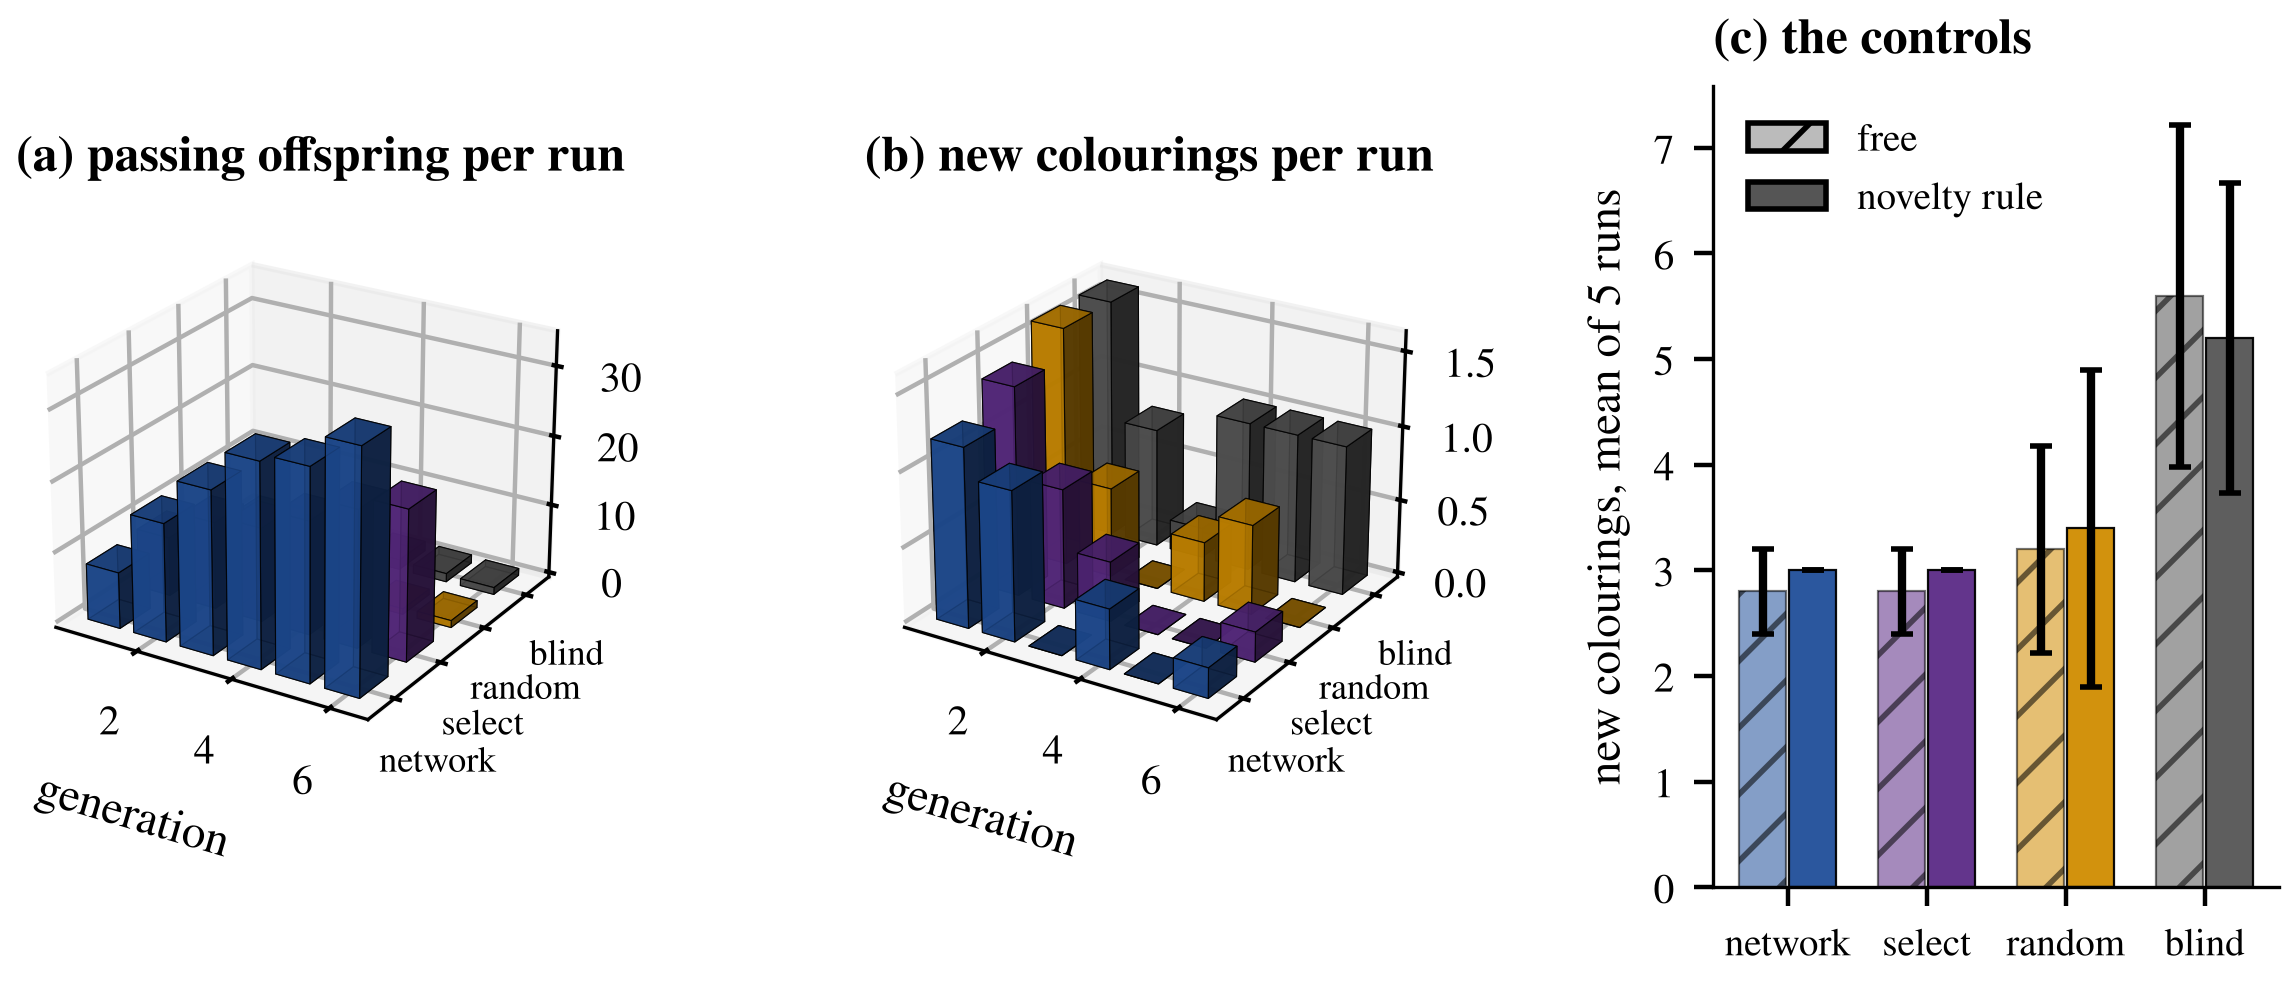
\includegraphics[width=0.98\textwidth]{figures/fig_crossing}
\Description{Curves of offspring passing the check and of new colourings per generation for the crossing network and its controls on Erdos problem 1183, and bars of new colourings per run.}
\caption{The crossing network against its controls on Erd\H{o}s problem 1183. (a) Offspring that pass the check, per generation, mean of five runs without the novelty rule. (b) Colourings not met before among them. (c) New colourings per run with and without the novelty rule, with one standard deviation. The network passes the most offspring and finds no more new colourings than the controls; the untyped arm finds the most.}
\label{fig:crossing}
\end{figure*}

\begin{table}[t]
\caption{The arms of the crossing network, five runs of $1200$ checks each. ``Pass'' is the share of offspring that pass the check; ``new'' is the number of new colourings per run (mean $\pm$ standard deviation) and ``optimal'' the number of them with $m(n)=f(n)$ for $n=6,\dots,9$. Ill-typed offspring are those of the blind arm that fail the typing.}
\label{tab:crossing}
\centering
\footnotesize
\setlength{\tabcolsep}{3.5pt}
\begin{tabular}{@{}lrrrr@{}}
\toprule
Arm & Pass & New & Optimal & Ill-typed \\
\midrule
\multicolumn{5}{@{}l}{\emph{free}}\\
network & $58.7\%$ & $2.8\pm0.4$ & $1.8$ & $0$ \\
select & $38.1\%$ & $2.8\pm0.4$ & $2.0$ & $0$ \\
random & $3.6\%$ & $3.2\pm1.0$ & $0.8$ & $0$ \\
blind & $2.7\%$ & $5.6\pm1.6$ & $1.6$ & $927$ \\
\multicolumn{5}{@{}l}{\emph{novelty rule}}\\
network & $1.3\%$ & $3.0\pm0.0$ & $2.0$ & $0$ \\
select & $1.4\%$ & $3.0\pm0.0$ & $2.0$ & $0$ \\
random & $1.4\%$ & $3.4\pm1.5$ & $1.0$ & $0$ \\
blind & $2.2\%$ & $5.2\pm1.5$ & $1.4$ & $1002$ \\
\bottomrule
\end{tabular}
\end{table}

\emph{The result} (Table~\ref{tab:crossing}). Without the novelty rule the network passes $58.7\%$ of its offspring against $3.6\%$ for random typed crossing, but almost all of them are colourings it has already found under another genome: it finds $2.8$ new colourings per run against $3.2$ for random crossing and $5.6$ for blind crossing. Under the novelty rule the pass rates fall to between $1.3\%$ and $2.2\%$ and the order of the new colourings is unchanged. The learned model therefore learns to repeat survivors, and it does not beat the random controls in the quantity that matters. Blind crossing does best because an untyped exchange occasionally grafts a family where a word was expected and so reaches combinations of the operations that typed crossing never proposes; the typing removes ill-formed genomes and, with them, part of the reachable set. None of the bred colourings improves a known value: the best, from the random arm, has $m(n)=7,7,8,8,9$ for $n=10,\dots,14$, which equals $f(n)$ at $n=11,13$ and exceeds it by one at $n=10,12,14$.

\emph{What did move the frontier} was a change of representation, not breeding. The optimal colourings found for $n=7,9,10$ by a counterexample-guided search over all colourings are level colourings, in which the colour of $S$ depends only on $|S|$; such a colouring is a word $c_{0}c_{1}\cdots c_{n}$, with colour classes $L_{0},L_{1}\subseteq\{0,\dots,n\}$. A \emph{weighted poset} is a finite poset $P$ with a map $w\colon P\to\{1,2,\dots\}$; $J(P)$ is its lattice of down-sets and $w(I)=\sum_{p\in I}w(p)$.

\begin{figure*}[t]
\centering
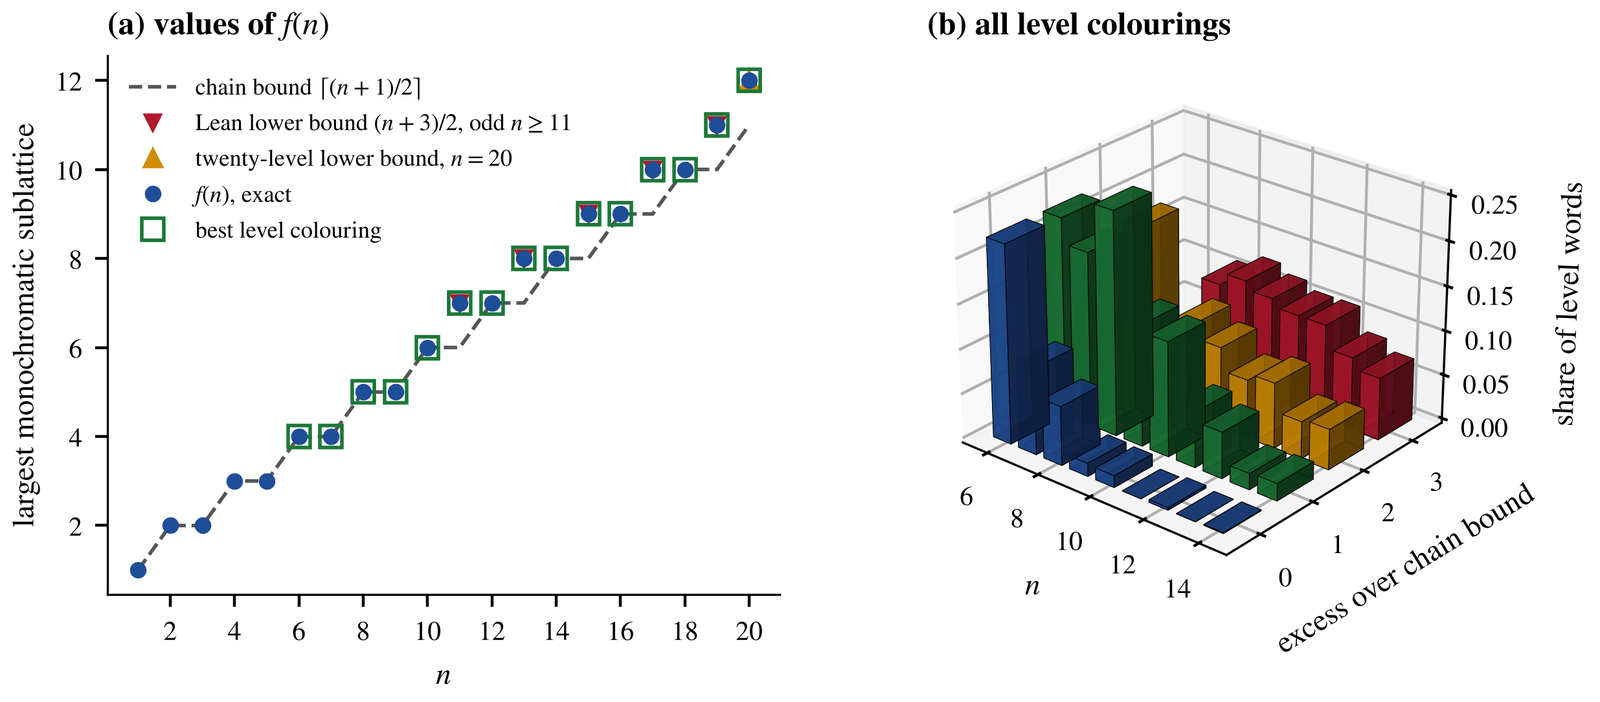
\includegraphics[width=0.98\textwidth]{figures/fig_sublattice}
\Description{The exact values of f(n) for n up to 20 against the chain bound and other bounds, and the distribution of the largest monochromatic sublattice over level colourings.}
\caption{Monochromatic sublattices of colourings of $2^{[n]}$. (a) The exact values of $f(n)$ for $n\le20$ (Theorem~\ref{thm:fvalues}), the chain bound $\lceil(n+1)/2\rceil$, the Lean lower bound $(n+3)/2$ for odd $n\ge11$ \cite{ORf1183}, the twenty-level lower bound $12$ at $n=20$, and the best level colouring, which attains $f(n)$ for every $n\le20$. (b) The distribution of the largest monochromatic sublattice over all level colourings for $6\le n\le14$, by its excess over the chain bound; the share of words that attain the bound falls quickly with $n$, and from $n=11$ on no odd word does.}
\label{fig:sublattice}
\end{figure*}

\begin{lemma}\label{lem:levelposet}
A level colouring has a monochromatic sublattice of colour class $L$ with $N$ members if and only if there are a weighted poset $(P,w)$ and an integer $t\ge0$ with $t+w(P)\le n$, $|J(P)|=N$ and $t+w(I)\in L$ for every $I\in J(P)$.
\end{lemma}

\begin{proof}
Let $D$ be a sublattice of $2^{[n]}$ with $N$ members whose sizes lie in $L$. It is a finite distributive lattice, so by Birkhoff's theorem it is isomorphic to $J(P)$ for the poset $P$ of its join-irreducible members, by the map that sends $A\in D$ to the set of join-irreducibles below it. The function $A\mapsto|A|$ is strictly increasing on $D$ and modular, since $|A\cup B|+|A\cap B|=|A|+|B|$. Write $p_{*}$ for the unique lower cover of a join-irreducible $p$ and $w(p)=|p|-|p_{*}|\ge1$. If $I$ is a down-set and $p$ a minimal element of $P\setminus I$, then $I\cup\{p\}$ is the join of $I$ and the principal down-set of $p$, and their meet is that principal down-set without $p$, which corresponds to $p_{*}$, so modularity gives $|I\cup\{p\}|=|I|+w(p)$; induction along a maximal chain of down-sets gives $|A|=t+w(I)$ with $t=|\min D|$, and $t+w(P)=|\max D|\le n$. Conversely, given $(P,w,t)$, choose disjoint sets $T$ and $B_{p}$ $(p\in P)$ in $[n]$ with $|T|=t$ and $|B_{p}|=w(p)$; the map $I\mapsto T\cup\bigcup_{p\in I}B_{p}$ is injective, carries unions and intersections of down-sets to unions and intersections of sets, and gives $I$ the size $t+w(I)\in L$.
\end{proof}

The lemma replaces the search over sublattices of $2^{[n]}$ by a search over weighted posets, which is small: the elements of $P$ are added in the order of the weights of their principal down-sets, each new element is placed above a down-set already built and creates the down-sets $I\cup\{p\}$ for every $I$ above that one, and a branch stops as soon as a new size leaves $L$. On $120$ random level colourings with $3\le n\le9$ the poset search and the general search agree on the largest monochromatic sublattice in every case, and on $30$ at $n=10$ they agree on every value below the cap of the poset search. A grid version, for colourings that depend on the sizes of $S$ in the blocks of a fixed partition of $[n]$, holds with weights in $\NN^{k}\setminus\{0\}$ by the same proof.

\begin{theorem}\label{thm:fvalues}
For $1\le n\le 19$,
\[
f(n)=\begin{cases}\lceil (n+1)/2\rceil & \text{if } n\le 10 \text{ or } n \text{ is even},\\[2pt] (n+3)/2 & \text{if } n\ge 11 \text{ is odd},\end{cases}
\]
and $f(20)=12$. For $11\le n\le20$ the value is attained by the level colouring of the word in the table below.
\begin{center}\small
\begin{tabular}{@{}rl@{\qquad}rl@{}}
$n$ & word $c_{0}\cdots c_{n}$ & $n$ & word $c_{0}\cdots c_{n}$\\
\midrule
$11$ & \texttt{110111001000} & $16$ & \texttt{10011001011100100}\\
$12$ & \texttt{1010011100100} & $17$ & \texttt{110100111001101000}\\
$13$ & \texttt{10111001101000} & $18$ & \texttt{0011001011100110100}\\
$14$ & \texttt{011010011100100} & $19$ & \texttt{00110010111000101101}\\
$15$ & \texttt{1100111010011000} & $20$ & \texttt{000101100111001011100}
\end{tabular}
\end{center}
\end{theorem}

\begin{proof}
The lower bounds are the chain bound and, for odd $n\ge11$, the theorem that every colouring then has a monochromatic sublattice with $(n+3)/2$ members, proved in Lean~4 by the OpenRefute project \cite{ORf1183}. For $n\le10$ the upper bound is attained by explicit colourings with no monochromatic sublattice of $\lceil(n+1)/2\rceil+1$ members, each checked by an exact search and by a satisfiability query that shares no code with it. For $11\le n\le19$ the words of the table have, by Lemma~\ref{lem:levelposet} and the exhaustive poset search, no monochromatic sublattice larger than the stated value; for $n=11$ this is confirmed by the exact search over all sublattices and by a satisfiability query. For $n=20$ the poset search finds $59$ level colourings of $2^{[20]}$, up to reversal and exchange of the colours, with no monochromatic sublattice of $13$ members, and the lower bound $f(20)\ge12$ is the twenty-level window of the footnote, which at $n=20$ gives a red and a blue sublattice with $23$ members together.
\end{proof}

The theorem answers the second part of the question of the footnote in the negative from $n=11$ on, as OpenRefute already did, and leaves the first open. Among level colourings (Fig.~\ref{fig:sublattice}) the chain bound is attained for every even $n\le18$ and exceeded by one for every odd $n$ from $11$ to $19$; up to reversal and exchange of the colours there are $9,7,6,8,3,2$ optimal words for $n=8,10,12,14,16,18$, and none for $n=20$, where the best level colouring has $12$ members against the chain bound $11$, and $12$ is $f(20)$. No optimal word for $n=8$ extends, two letters at a time on the right, through optimal words to $n=18$. The lemma shows the obstruction: three sizes of one colour in arithmetic progression already give a sublattice with one member more than the sizes, and a progression of length $d+1$ gives $2^{d}$ members, so a good word must avoid long monochromatic progressions in each colour class while the number of its colour changes grows with $n$. At $n=20$ no colouring at all attains the chain bound.

\emph{What the experiment shows.} The chain reaction was asked to produce new constructions faster than random crossing, and it did not; its survival model learned to propose what had already survived. The one advance on the problem came from a proof, Lemma~\ref{lem:levelposet}, that changed what could be checked: it turned the general search, which reaches $n=11$, into a search over weighted posets, which reaches $n=20$. In the terms of Theorem~\ref{thm:I}, the network sharpened the profile of a proposer whose support did not contain the needed idea; the lemma enlarged the support.

\subsection{Yang--Mills and Hodge: crossing on the open steps}\label{ssec:headline}

The crossing network of the package (Section~\ref{ssec:crossing} describes it on a calibration problem) is aimed here at the open leaves of the two trees. Every construction of its library is a typed node: it gives an output of one type and needs inputs of others. The Yang--Mills library holds the single-link law of $\mathrm{SU}(2)$, which is a von Mises--Fisher law on $S^{3}$; the sharp quarter inequality $W_{1}(\nu_{b},\nu_{b'})\le\frac14|b-b'|$ of \cite{BB26d}; Dobrushin's uniqueness criterion \cite{Dob68}; three dependency graphs of the links (no gauge fixing, temporal gauge, and the maximal-tree gauge of Creutz \cite{Cre77} with one fixed link in every plaquette); reflection positivity and the transfer matrix \cite{OSei78}; the gauge Dobrushin--Shlosman criterion and the Bakry--\'Emery bound of \cite{SZZ23}; the Polchinski flow and the multiscale log-Sobolev inequality \cite{BB21}; Ba{\l}aban's renormalisation group \cite{Bal87}; and a finite subgroup of $\mathrm{SU}(2)$. The Hodge library holds Markman's theorem on Weil classes of abelian fourfolds \cite{Mar25w}, the reduction of Moonen and Zarhin in dimension at most five \cite{MZ98}, Schoen's products \cite{Sch98p}, Shioda's structure of Fermat varieties \cite{Shi79}, the Hodge characters of the Fermat fourfold of degree $110$ left by the census of \cite{BB26c}, Buskin's theorem on Hodge isometries of K3 surfaces \cite{Bus19}, and an unrefereed claim of the Hodge conjecture for CM abelian varieties \cite{OAI26b}. Two nodes cross when the output of one is an input of the other. An offspring that needs nothing more is closed and goes to its check, a computation that accepts, rejects with the measurement that stopped it, or stops when no checkable form exists. Checked offspring join the pool and seed the next generation.

\begin{figure*}[t]
\centering
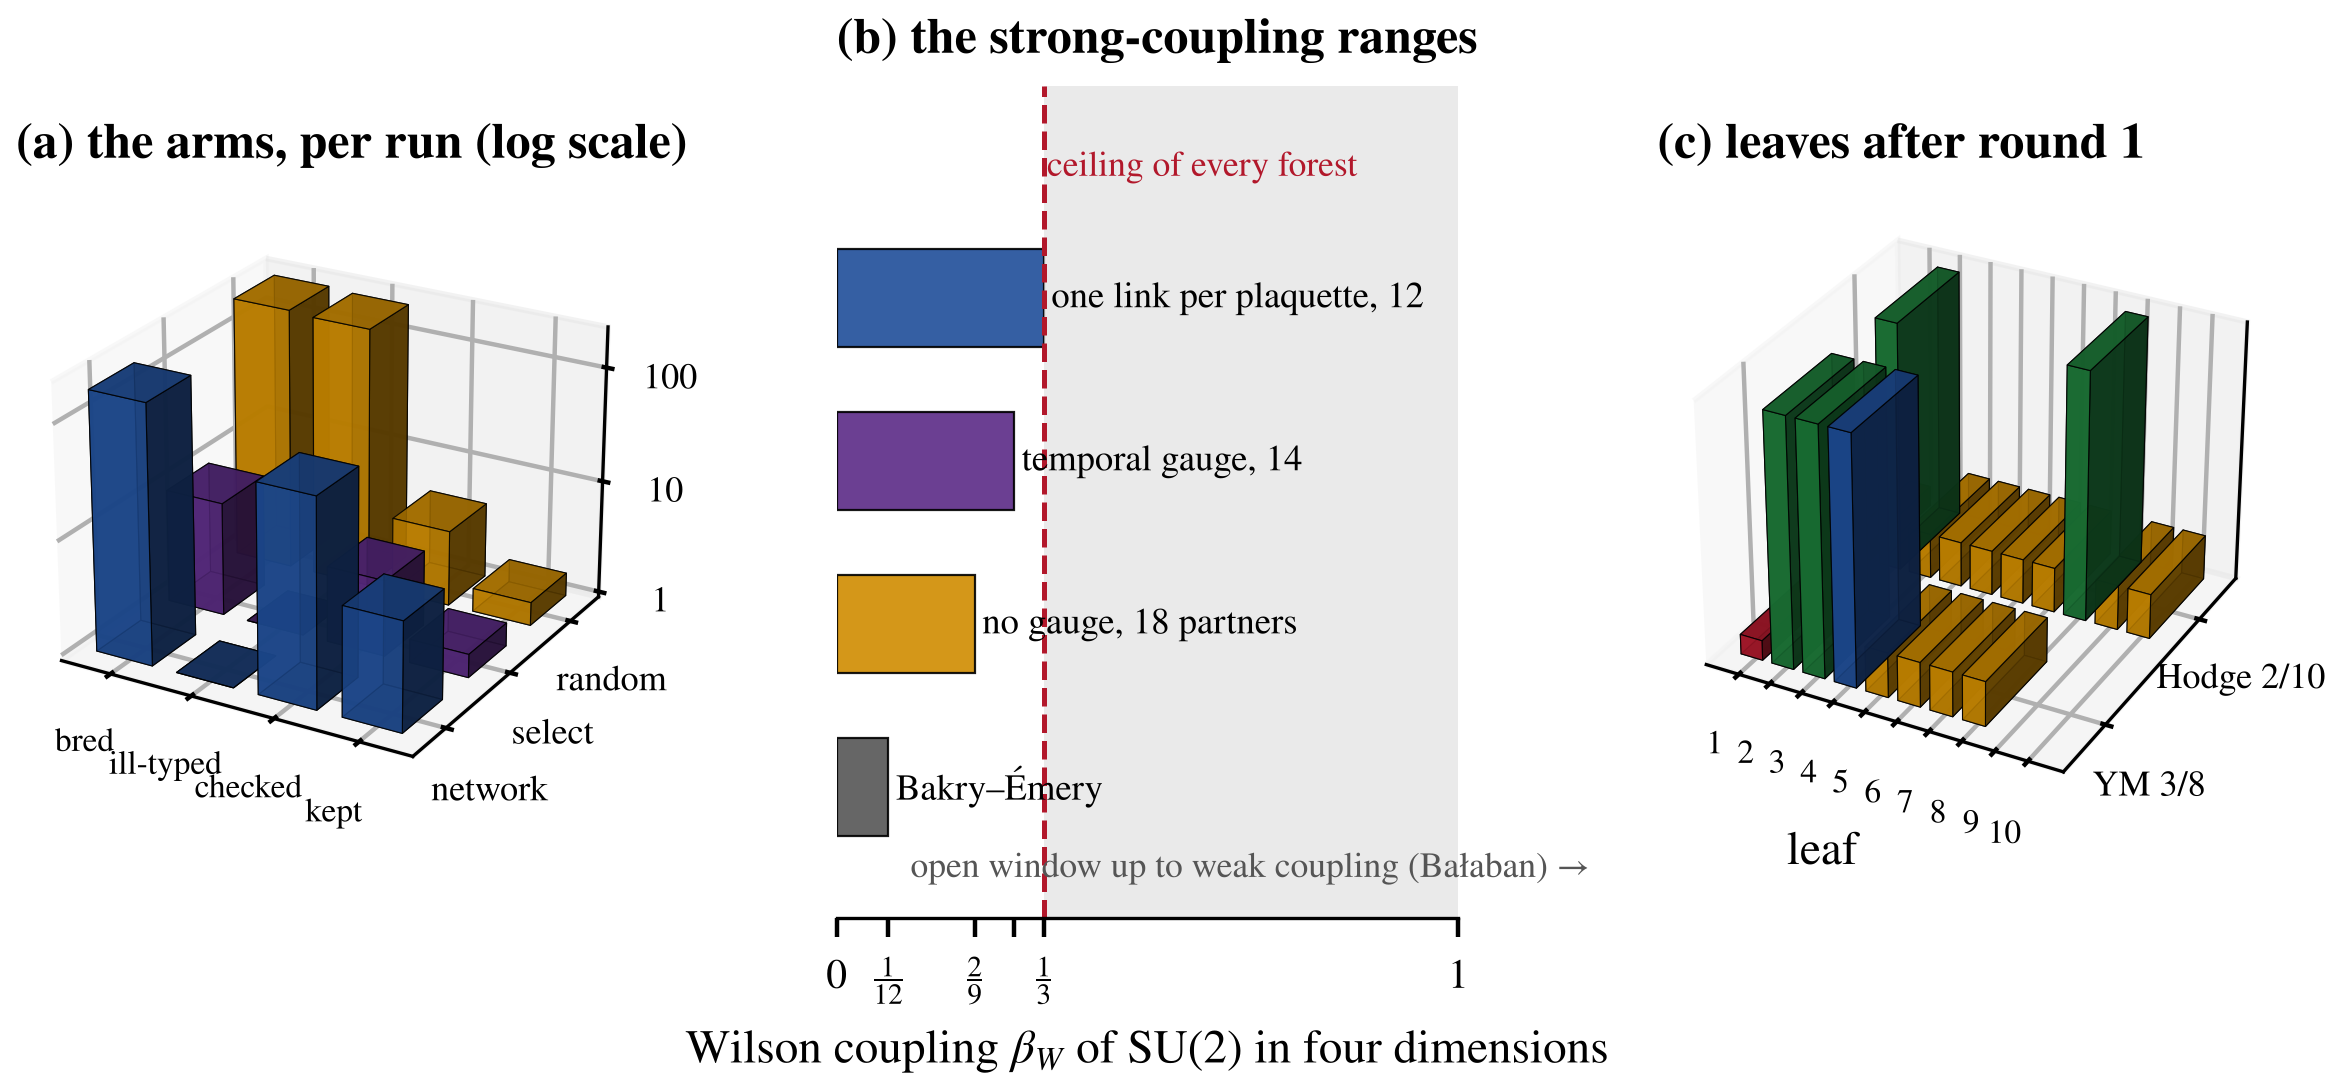
\includegraphics[width=0.98\textwidth]{figures/fig_headline}
\caption{The first headline round. (a) Offspring bred, ill-typed, checked and kept per run of each arm, on a logarithmic scale. The network enumerates the typed crosses; select draws pairs at random and keeps those whose types fit; random crosses whatever the types. (b) The ranges of four-dimensional $\mathrm{SU}(2)$ on which a lattice mass gap is proved: Bakry--\'Emery \cite{SZZ23}, single-link Dobrushin without gauge fixing \cite{BB26d}, and after the temporal and the one-per-plaquette gauge fixings (Theorem~\ref{thm:onethird}). The dashed line is the ceiling of every forest gauge fixing (Proposition~\ref{prop:forestceiling}); beyond it the window up to weak coupling is open. (c) The leaves of the two trees after the round, in the order of Table~\ref{tab:closure}: proved (green, the new step in blue), open (amber) and blocked (red).}
\label{fig:headline}
\end{figure*}

\emph{The first round.} Over five seeds of five generations of $40$ crosses, the network bred $180$ offspring per run, checked $64$ and accepted $8$; select bred $8.8$, checked $3.6$ and accepted $0.6$; random bred $200$, of which $191.2$ were ill-typed, and accepted $0.6$ (Fig.~\ref{fig:headline}a). Every run of the network reached the composite of Dobrushin's criterion, the sharp quarter, the von Mises--Fisher law and the maximal-tree gauge, whose check counts $12$ active partners for every active link and accepts the range $\beta_{W}<\frac13$; no run of the controls reached it. The network enumerates every typed pair, so its runs do not depend on the seed. The composite was first proposed by the language-model proposer of the package, which suggested fixing a gauge to cut the number of partners; a satisfiability search found the pattern of Lemma~\ref{lem:forest}, Lean~4 checked its finite part, and the cross was then entered in the library, from which the network rederives it. The network therefore reproduces this step; it did not originate it.

\emph{The step.} We use the normalisation of \cite{SZZ23,BB26d}: the Wilson measure of $\mathrm{SU}(2)$ on a finite set of links has density $\exp(2\beta\sum_{p}\mathrm{Re}\,\mathrm{Tr}\,U_{p})$ with respect to Haar measure, where $U_{p}$ is the ordered product around the plaquette $p$, and $\beta_{W}=4\beta$ is the coupling of the physics literature. A link of $\mathbb{Z}^{4}$ is written $(x,\mu)$ for the pair $\{x,x+e_{\mu}\}$; the plaquette at $x$ in the plane $\mu<\nu$ consists of the links $(x,\mu)$, $(x+e_{\mu},\nu)$, $(x+e_{\nu},\mu)$, $(x,\nu)$.

\begin{lemma}\label{lem:forest}
Let $\sigma\colon(\mathbb{Z}/2)^{4}\to\{0,1,2,3\}$ take the values $0,0,2,3,3,1,2,1,1,2,1,3,3,2,0,0$ at $x_{0}+2x_{1}+4x_{2}+8x_{3}=0,1,\dots,15$, and let $F$ be the set of links $(x,\sigma(x\bmod2))$, $x\in\mathbb{Z}^{4}$. Then
\begin{enumerate}[label=\textup{(\roman*)},leftmargin=*,itemsep=0pt]
\item every plaquette of $\mathbb{Z}^{4}$ contains exactly one link of $F$;
\item $F$ is a forest, and so is $F\cap E(\Lambda)$ for every set $\Lambda$ of sites, $E(\Lambda)$ being the links with both ends in $\Lambda$;
\item every link $e\notin F$ shares a plaquette with exactly $12$ links not in $F$, two in each of its six plaquettes.
\end{enumerate}
\end{lemma}

\begin{proof}
(i) The plaquette at $x$ in the plane $\mu<\nu$ contains $\#\{\sigma(x)\in\{\mu,\nu\}\}+[\sigma(x+e_{\mu})=\nu]+[\sigma(x+e_{\nu})=\mu]$ links of $F$, a number that depends only on $x\bmod2$ and the plane; inspection of the $16\times6=96$ cases of the table gives $1$ in each.\footnote{The inspection is a finite check. The eBLLM package carries it out in Lean~4, in the theorem \lean{one\_fixed\_per\_plaquette} of its file \lean{EBLLM/GaugeFix.lean}, proved by \lean{decide}, and repeated independently on a box of side six by \lean{verify\_gauge.py}. The table was found by a satisfiability search over the $4^{16}$ functions $\sigma$; it has eight solutions of period two, and none of period three.} (ii) Every site $x$ has exactly one link of $F$ leaving it in the positive direction, the link to $x+e_{\sigma(x)}$, and that link raises $h(x)=x_{0}+x_{1}+x_{2}+x_{3}$ by one. In a cycle of $k$ links of $F$ on $k$ sites, each link is the positive link of one of its ends and each site has at most one positive link, so each site of the cycle is the lower end of exactly one of its links and the cycle is directed; then $h$ increases strictly around it, which is impossible. A subgraph of a forest is a forest. (iii) A link lies in six plaquettes; by (i) each of them has exactly one link of $F$, which is not $e$, so it has two active links besides $e$. Two distinct plaquettes meet in at most one link, so the $12$ partners are distinct.
\end{proof}

On a periodic box $(\mathbb{Z}/L\mathbb{Z})^{4}$ the set $F$ contains cycles, since $h$ is not defined modulo $L$, and the argument below never uses a periodic box. Let $\gamma^{F}$ be the specification on the links of $\mathbb{Z}^{4}$ not in $F$ with a priori Haar measure and formal density $\exp(2\beta\sum_{p}\mathrm{Re}\,\mathrm{Tr}\,U^{F}_{p})$, where $U^{F}_{p}$ is the plaquette product with the links of $F$ replaced by $1$; for a box $\Lambda$ let $\mu^{F}_{\Lambda}$ be the finite-volume measure on the active links of $\Lambda$ with the plaquettes of $\Lambda$ only, and $W_{\Lambda}$ the Wilson measure on $E(\Lambda)$ with free boundary.

\begin{theorem}[Gauge-fixed strong coupling]\label{thm:onethird}
For four-dimensional $\mathrm{SU}(2)$ with $0\le\beta_{W}<\frac13$:
\begin{enumerate}[label=\textup{(\roman*)},leftmargin=*,itemsep=0pt]
\item $\gamma^{F}$ has exactly one Gibbs measure $\mu_{F}$, and its truncated correlations of Lipschitz local functions decay exponentially with every rate $\lambda<-\log(3\beta_{W})$ in the distance of their supports;
\item for every gauge-invariant local function $O$ the limit $\omega(O)=\lim_{\Lambda}W_{\Lambda}(O)$ exists along every sequence of boxes that exhausts $\mathbb{Z}^{4}$, and $\omega(O)=\mu_{F}(O^{F})$, where $O^{F}$ is $O$ with the links of $F$ set to $1$;
\item $\omega$ is invariant under translations and the hypercubic group and reflection positive, and its transfer matrix has a spectral gap $m\ge-\log(3\beta_{W})$.
\end{enumerate}
\end{theorem}

\begin{proof}
(i) The conditional law of an active link $e$ under $\gamma^{F}$ is the von Mises--Fisher law $\nu_{b}$ with $b=4\beta$ times the sum of the six staples of $e$, each staple being the product of the other links of a plaquette through $e$, with the links of $F$ equal to $1$. Moving an active link $e'$ moves at most one staple of $e$, since two links share at most one plaquette, and moves it by an isometric image of the displacement, since multiplication by unit quaternions is an isometry of $\RR^{4}$. By the sharp quarter inequality \cite[Theorem~A]{BB26d} the Dobrushin coefficient in the chordal metric of $S^{3}$ satisfies $C_{ee'}\le4\beta\cdot\frac14=\beta$, and $C_{ee'}=0$ unless $e'$ is one of the $12$ partners of Lemma~\ref{lem:forest}(iii). Every row and column of $C$ therefore sums to at most $\alpha=12\beta=3\beta_{W}<1$, and the Kantorovich--Dobrushin comparison lemma of \cite[Appendix]{BB26d} gives uniqueness and decay at every rate $\lambda<-\log\alpha$, exactly as in the proof of \cite[Theorem~E]{BB26d}.

(ii) Fix a box $\Lambda$. By Lemma~\ref{lem:forest}(ii) the set $F_{\Lambda}=F\cap E(\Lambda)$ is a finite forest. Root each of its trees and, given the values $U_{F}$ on $F_{\Lambda}$, define $g\colon\Lambda\to\mathrm{SU}(2)$ by $g=1$ at the roots and, along each tree, $g_{y}=g_{x}U_{xy}$ for every link $(x,y)$ of the tree; this is consistent because the tree has no cycle, and it makes $g_{x}U_{xy}g_{y}^{-1}=1$ on $F_{\Lambda}$. For fixed $U_{F}$ the map $U_{e}\mapsto g_{x}U_{e}g_{y}^{-1}$ on the active links is a product of left and right translations and preserves Haar measure, and the Wilson action is gauge invariant. Hence under $W_{\Lambda}$ the gauge-transformed active links are independent of $U_{F}$ and have law $\mu^{F}_{\Lambda}$, and $W_{\Lambda}(O)=\mu^{F}_{\Lambda}(O^{F})$ for gauge-invariant $O$. No holonomy is left over, because $F_{\Lambda}$ has no cycle. Now let $\Lambda\subset\Lambda'$ be boxes and compare $\mu^{F}_{\Lambda'}$ with $\mu^{F}_{\Lambda}\otimes\mathrm{Haar}$ on the active links of $\Lambda'$. Both are invariant under the single-link resampling of $\mu^{F}_{\Lambda'}$ at every active link all of whose plaquettes lie in $\Lambda$; the remaining links form a set $S$ within distance one of the complement of $\Lambda$. The comparison lemma of \cite[Appendix]{BB26d}, with $\theta=\alpha e^{\lambda}<1$, couples the two measures so that the expected distance on the support $T$ of $O^{F}$ is at most $\frac{2\theta}{1-\theta}\sum_{z\in S}e^{-\lambda\,\mathrm{dist}(z,T)}\le c_{T}\,R^{3}e^{-\lambda R}$, with $R=\mathrm{dist}(T,\mathbb{Z}^{4}\setminus\Lambda)$ and $c_{T}$ independent of $\Lambda'$. As $O^{F}$ is Lipschitz, $|W_{\Lambda'}(O)-W_{\Lambda}(O)|\le c_{O}R^{3}e^{-\lambda R}$. Any two boxes that contain the support at distance $R$ lie in a common larger box, so $W_{\Lambda}(O)$ converges along every exhausting sequence to one limit $\omega(O)$. The same coupling with $\mu_{F}$ in place of $\mu^{F}_{\Lambda'}$, which is invariant under all single-link resamplings of $\gamma^{F}$, gives $\omega(O)=\mu_{F}(O^{F})$.

(iii) For a translation or a symmetry $\tau$ of the lattice, $W_{\Lambda}(O\circ\tau)=W_{\tau\Lambda}(O)$ by the symmetry of the Wilson action, and the boxes $\tau\Lambda$ also exhaust $\mathbb{Z}^{4}$; by (ii) the limit is $\omega(O)$. Only the boxes move, not $F$. For a reflection $\vartheta$ in a lattice hyperplane through sites or bisecting links, the free-boundary measures $W_{\Lambda}$ on boxes symmetric under $\vartheta$ are reflection positive \cite{OSei78}, and by (ii) $\omega$ is their limit, so $\omega(\vartheta(\bar G)G)\ge0$ for every local $G$ supported on one side. Finally, for a gauge-invariant Lipschitz $G$ supported at times in $[0,s]$, part (i) applied to $\vartheta(\bar G)^{F}$ and $(\tau_{t}G)^{F}$, whose supports are at distance at least $t-s-1$, gives $0\le\omega(\vartheta(\bar G)\tau_{t}G)-|\omega(G)|^{2}\le C_{G}e^{-\lambda t}$. Such functions are dense in $L^{2}(\omega)$ on each bounded time interval, so \cite[Proposition~gapdecay]{BB26d} gives a gap at least $\lambda$ for every $\lambda<-\log(3\beta_{W})$.
\end{proof}

The theorem extends \cite[Theorem~F]{BB26d}, where the range is $\beta_{W}<\frac29$ and the state is the limit of periodic boxes, to $\beta_{W}<\frac13$, with the state the limit of free boxes. It has been checked here and not refereed. A search of the literature on strong-coupling expansions found no earlier statement of this range: \cite{OSei78} and the cluster expansions that followed give convergence at strong coupling without an explicit Dobrushin range, \cite{SZZ23} gives $\beta_{W}<\frac1{12}$, and the Lean project of strong-coupling lattice gauge theory cited in \cite{BB26d} has $\beta<1/(32n(d-1))$.\footnote{The search covered the arXiv listings in math-ph, hep-lat and math.PR, the citations of \cite{SZZ23}, the gauge-fixed formulations of Ba{\l}aban's renormalisation group, and the expository literature on maximal-tree gauges after \cite{Cre77}. The monograph of Seiler on gauge theories as statistical mechanics could not be read from the session, and its strong-coupling results are cluster expansions without an explicit range of the Dobrushin type.} The gain over \cite{BB26d} comes from the dependency graph and not from the metric: after a forest gauge fixing a plaquette has three active links instead of four, and each link loses six of its $18$ partners.

\begin{proposition}[The ceiling of forest gauge fixings]\label{prop:forestceiling}
Let $F'$ be any set of links of $\mathbb{Z}^{4}$ whose intersection with every box is a forest. Then the single-link Dobrushin coefficients of $\gamma^{F'}$, in the chordal or the geodesic metric of $S^{3}$, have $\sup_{e}\sum_{e'}C_{ee'}\ge12\beta$. Hence no single-link Dobrushin argument after a forest gauge fixing proves uniqueness for $\beta_{W}\ge\frac13$.
\end{proposition}

\begin{proof}
In a box of side $n$ there are $n^{4}$ sites, $4n^{4}-O(n^{3})$ links and $6n^{4}-O(n^{3})$ plaquettes, and a forest has at most $n^{4}-1$ links, so at least $3n^{4}-O(n^{3})$ links are active. Let $a_{p}$ be the number of active links of the plaquette $p$; then $\sum_{p}a_{p}=6\cdot\#\{\text{active links}\}-O(n^{3})$, since every link lies in six plaquettes, and the mean $\bar a$ of $a_{p}$ is at least $3-o(1)$. An active link $e$ has $\sum_{p\ni e}(a_{p}-1)$ active partners, so the sum of the partner counts over the active links is $\sum_{p}a_{p}(a_{p}-1)\ge\sum_{p}a_{p}\,(\bar a-1)$ by the Cauchy--Schwarz inequality, and the mean partner count is at least $6(\bar a-1)\ge12-o(1)$. Partner counts are integers, so some active link has at least $12$ partners. For each partner $e'$ of such a link, the staples of $e$ involve pairwise disjoint sets of other links and can be chosen with sum zero while the staple through $e'$ is arbitrary, and the proof of \cite[Proposition~ceiling]{BB26d} gives $C_{ee'}\ge\beta$.
\end{proof}

Passing to a weighted Dobrushin condition does not help either, since the spectral radius of a nonnegative matrix is at least its mean row sum over a box, up to the boundary.

\emph{The amplified round.} The second round adds to the library the crosses aimed at the assumption of each ceiling, the partners of the gauge-fixed specification, and the nodes obtained by transferring the pattern of the step that moved, \emph{remove redundant variables by a symmetry, then apply a local criterion}. It also passes every accepted offspring through a refuter before it counts, and adds the booster layer described below. Up to depth four the library breeds $21{,}515$ composites, of which $1{,}466$ are closed. Of these, $934$ stop without a checkable form, $433$ are rejected by their check, and $99$ are accepted. The refuter breaks $35$ of the accepted ones, $26$ because a stronger range is already known and $9$ because they reproduce an accepted range with no gain, and $64$ survive (Table~\ref{tab:amplify}).
\begin{itemize}[leftmargin=*,itemsep=1pt]
\item \emph{Plaquette variables} \cite{Bat82}. In these variables the Bianchi identity of each cube fixes every plaquette variable, up to parallel transport, by the other five plaquettes of the cube. The single-variable kernels are therefore point masses, so Dobrushin's coefficients equal one and the cross is rejected.
\item \emph{Blocks of active links.} A block coefficient needs the Kantorovich sensitivity of the joint law of a block at finite $\beta$, and the sharp quarter does not control it; the cross stops.
\item \emph{Path coupling.} The single-link Glauber dynamics contracts on exactly the Dobrushin range, so the cross gains nothing.
\item \emph{Bakry--\'Emery after the forest gauge fixing.} The Hessian of $\mathrm{Re}\,\mathrm{Tr}$ of a product of $k$ active links is at most $2k$ times the squared norm of the tangent vector. With three active links per plaquette instead of four, the curvature condition of \cite{SZZ23} improves from $\beta_{W}<\frac1{12}$ to $\beta_{W}<\frac19$, which the Dobrushin range dominates.
\item \emph{Dobrushin--Shlosman on a box of the gauge-fixed specification.} This needs the sensitivity of a box law to its boundary at order-one coupling, an integral over $\mathrm{SU}(2)^{3n^{4}}$; the estimate of \cite{BB26d} puts the box side near $90$, and the cross stops.
\item \emph{Pattern transfer to Fermat fourfolds.} Shioda's criterion is invariant under $\mu_{m}^{6}\rtimes S_{6}$ and under the Galois group. The leftover character $(1,16,26,31,36)$ at level $55$ has an orbit of $8$ members under the units of $\mathbb{Z}/55$, and none of them splits into zero-sum pairs and triples, so the quotient by the symmetries gives nothing new.
\item \emph{Pattern transfer to K3 squares.} For a K3 surface $S$ with real multiplication by $\mathbb{Q}(\sqrt d)$, the element $\sqrt d$ is a Hodge similitude $T(S)\to T(S)(d)$ and not an isometry, so Buskin's theorem does not apply to it. Composites through K3 surfaces $S'$ with $T(S')\cong T(S)(d)$ are similitudes too. Varesco reduces the algebraicity of Hodge similitudes to the Kuga--Satake Hodge conjecture \cite{Var23}, and he proves it on the first four-dimensional families. The transferred node therefore reproduces a known route, and it stops at the very general member of the larger families.
\end{itemize}

\begin{table}[t]
\caption{The amplified round on the two libraries, up to depth four. ``Survived'' counts accepted composites that the refuter could not break. The surviving Yang--Mills composites are $18$ forms each of the gap for $\beta_{W}<\frac29$, $<\frac27$ and $<\frac13$, and $3$ of uniqueness in each range; the Hodge survivor is (F2) in dimension at most five, which was known.}
\label{tab:amplify}
\centering
\footnotesize
\setlength{\tabcolsep}{4pt}
\begin{tabular}{@{}lrrrrr@{}}
\toprule
& Closed & Stopped & Rejected & Refuted & Survived \\
\midrule
Yang--Mills & $1{,}460$ & $932$ & $430$ & $35$ & $63$ \\
Hodge & $6$ & $2$ & $3$ & $0$ & $1$ \\
\midrule
Total & $1{,}466$ & $934$ & $433$ & $35$ & $64$ \\
\bottomrule
\end{tabular}
\end{table}

\subsection{Boosters}\label{ssec:boosters}

The booster layer of Section~\ref{sec:network} was tested on the Yang--Mills library at a budget at which no arm can enumerate every typed pair: $6$ crosses in each of $8$ generations, over $200$ seeds. Two forms were run, one synapse per pair of pool members and one per pair of library heads, so that a weight learned on one composite carries to every composite with the same heads; in a second experiment the boosted arm keeps its weights for four rounds (Fig.~\ref{fig:boosters}).

\begin{figure*}[t]
\centering
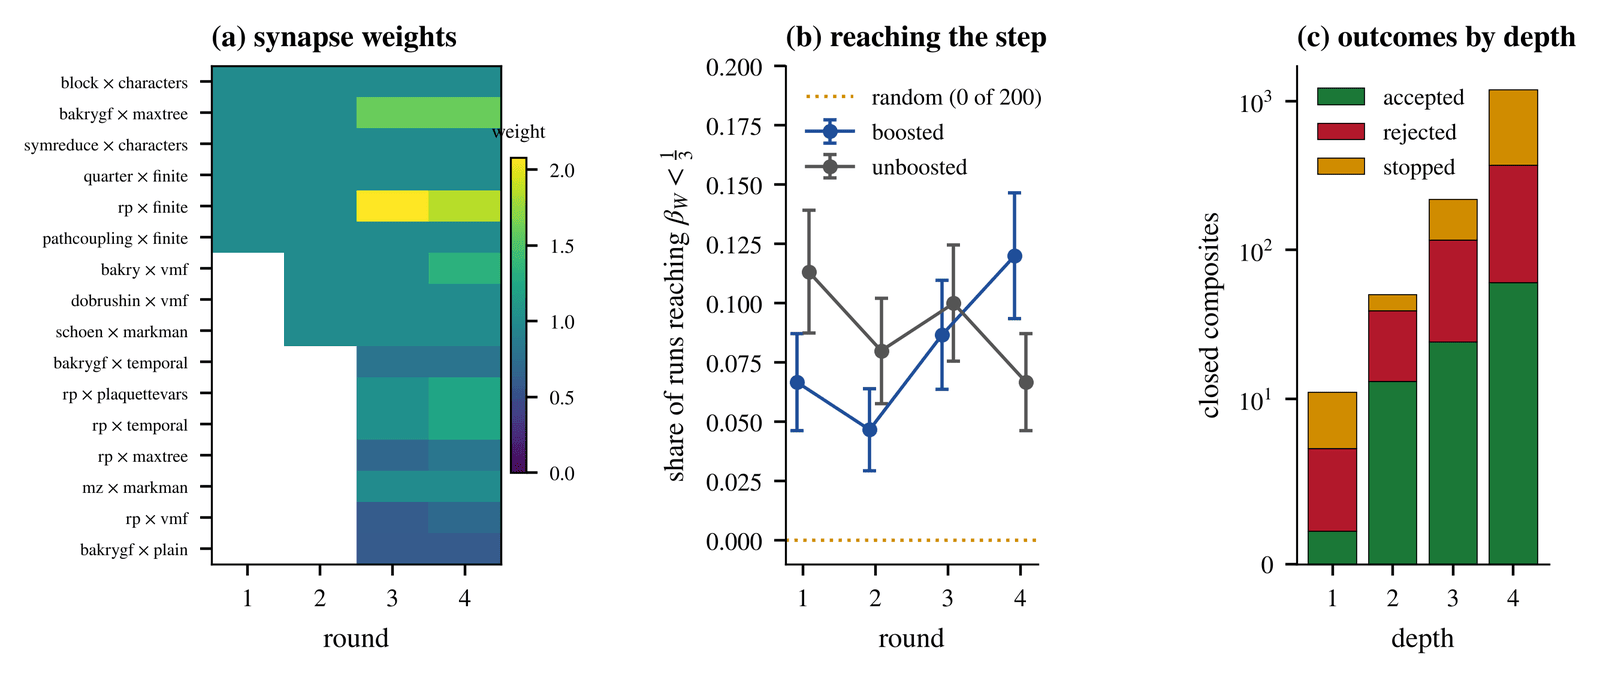
\includegraphics[width=0.98\textwidth]{figures/fig_boosters}
\caption{The booster layer. (a) The weights of the synapses of one boosted run over four rounds, one row per synapse; a blank cell is a synapse not yet created. (b) The share of $200$ runs that reach $\beta_{W}<\frac13$ within $48$ crosses, for the boosted arm that keeps its weights from round to round and for the unboosted network, with one standard error; random pairing never reaches it. (c) The outcomes of the $1{,}466$ closed composites of the amplified library, by depth.}
\label{fig:boosters}
\end{figure*}

\begin{table}[t]
\caption{Boosted, unboosted and random crossing at a budget of $48$ crosses, $200$ runs per arm. ``Reached $\frac13$'' counts runs whose survivors include $\beta_{W}<\frac13$, with the mean generation at which they reach it; survivors and refuted offspring are means per run.}
\label{tab:boosters}
\centering
\footnotesize
\setlength{\tabcolsep}{3.5pt}
\begin{tabular}{@{}llrrrr@{}}
\toprule
Synapse & Arm & Reached $\frac13$ & Generation & Survivors & Refuted \\
\midrule
pair & boosted & $14$ & $5.86$ & $0.61$ & $1.14$ \\
head & boosted & $12$ & $5.58$ & $0.62$ & $1.16$ \\
-- & unboosted & $21$ & $5.43$ & $0.68$ & $1.25$ \\
-- & random & $0$ & -- & $0.08$ & $0.05$ \\
\bottomrule
\end{tabular}
\end{table}

Boosters do not beat the unboosted network (Table~\ref{tab:boosters}). Within one round the boosted arms reach the step in $12$ and $14$ of $200$ runs against $21$ for the unboosted network; the difference is within two standard errors. Across four rounds the boosted share moves from $0.067$ to $0.12$ and the unboosted share from $0.113$ to $0.067$, again within two standard errors in every round. Both are far above random pairing, which wastes $45$ of its $48$ crosses on ill-typed pairs and never reaches the step. The reason is the one met in Section~\ref{ssec:crossing}: a booster strengthens synapses that have already fired, and the step that moved needed a synapse that had never fired, between Dobrushin's criterion and the maximal-tree gauge. The typing, not the learning, carries the advantage of the network.

\subsection{Gap numbers and the construction graph}\label{ssec:gapnumbers}

\emph{Gap numbers.} Each round reports two numbers. For Yang--Mills it is the largest coupling below which the lattice gap is proved, and its share of the interval up to $\beta_{W}\approx2.2$, where Monte Carlo simulations of four-dimensional $\mathrm{SU}(2)$ see the crossover from strong to weak coupling \cite{Cre80}; this is a physical marker and not the threshold of any proof, since Ba{\l}aban's control is not explicit in the coupling. The number moved from $\frac29$, or $10.1\%$, before the rounds to $\frac13$, or $15.2\%$, in the first round, and stayed there in the second. For Hodge it is, for each open family, the largest dimension of a family on whose general member the classes are known to be algebraic, against the dimension of the largest family of its kind (Table~\ref{tab:closure}). No Hodge number moved.

\begin{table*}[t]
\caption{The leaves of the two benchmark trees after the second round, with the result that settles a proved leaf, the check that stopped the last attempt on an open one, and, for the open families of the Hodge tree, the gap number: the largest dimension of a family on whose general member the classes are known to be algebraic, against the dimension of the largest family of its kind. Yang--Mills: $3$ of $8$ leaves proved ($37.5\%$); Hodge: $2$ of $10$ ($20\%$).}
\label{tab:closure}
\centering
\footnotesize
\setlength{\tabcolsep}{4pt}
\begin{tabular}{@{}rp{0.22\textwidth}p{0.08\textwidth}p{0.55\textwidth}p{0.07\textwidth}@{}}
\toprule
& Leaf & Status & Source, or what blocks & Gap \\
\midrule
\multicolumn{5}{@{}l}{\emph{Yang--Mills}}\\
\rr 1 & \rr a faithful Lean statement of the Clay problem & \rr blocked & \rr no formal statement of the Wightman axioms for a gauge theory exists to state it against & \rr -- \\
\rr 2 & \rr lattice gap at strong coupling & \rr proved & \rr $\beta_{W}<\frac29$ \cite{BB26d} & \rr -- \\
\rr 3 & \rr fine-scale control at weak coupling & \rr proved & \rr Ba{\l}aban's renormalisation group \cite{Bal87} & \rr -- \\
\rr 4 & \rr the window from below & \rr proved & \rr $\beta_{W}<\frac13$, Theorem~\ref{thm:onethird}; the ceiling of the method, Proposition~\ref{prop:forestceiling} & \rr $15.2\%$ \\
\rr 5 & \rr a finite-box mixing certificate in the window & \rr open & \rr the box needs side about $90$; no computation over $\mathrm{SU}(2)^{4n^{4}}$ at that size exists & \rr -- \\
\rr 6 & \rr a lift of the two-dimensional gap through dimension & \rr open & \rr no family of theories interpolating in dimension with a uniform gap is known & \rr -- \\
\rr 7 & \rr a multiscale log-Sobolev inequality at order-one coupling & \rr open & \rr the method of \cite{BB21} needs a Polchinski flow with uniformly convex effective potentials; for gauge fields none is known, and gauge invariance removes the Gaussian reference measure & \rr -- \\
\rr 8 & \rr the continuum limit with the Wightman axioms & \rr open & \rr needs a lattice gap uniform in the spacing, Hypothesis~R, which is the Clay problem on the lattice & \rr -- \\
\midrule
\multicolumn{5}{@{}l}{\emph{Hodge}}\\
\rr 1 & \rr a faithful Lean statement & \rr blocked & \rr Hodge classes and algebraic cycles of complex projective varieties are not yet formalised & \rr -- \\
\rr 2 & \rr (F2) in dimension at most five & \rr proved & \rr \cite{Mar25w,MZ98} & \rr -- \\
\rr 3 & \rr (F2) for CM abelian varieties & \rr open & \rr the only claim is unrefereed \cite{OAI26b}; the refuter rejects it & \rr -- \\
\rr 4 & \rr Weil classes on Weil eightfolds of nontrivial discriminant & \rr open & \rr no construction of the classes is known & \rr $0/16$ \\
\rr 5 & \rr a semiregular object on $E_{0}^{6}$ meeting the polarised criterion & \rr open & \rr every convolution tested in \cite{BB26c} has too large an $\mathrm{Ext}^{2}$ & \rr -- \\
\rr 6 & \rr Weil classes on Weil sixfolds & \rr open & \rr products of Weil fourfolds and Weil surfaces fill a family of dimension $5$ in the moduli of dimension $9$; a very general Weil sixfold is simple & \rr $5/9$ \\
\rr 7 & \rr (F3$'$) for $S\times S$, $S$ a K3 surface with real multiplication & \rr open & \rr $\sqrt d$ is a Hodge similitude; Varesco's reduction to the Kuga--Satake Hodge conjecture \cite{Var23} covers the first four-dimensional families, the largest family has dimension $8$ & \rr $4/8$ \\
\rr 8 & \rr Fermat fourfolds, degrees with split characters & \rr proved & \rr Shioda's zero-sum criterion \cite{Shi79} with the census of \cite{BB26c} & \rr -- \\
\rr 9 & \rr the Fermat fourfold of degree $110$ & \rr open & \rr the leftover character has a lattice point in its Fine interior, so no block family covers it, and its orbit under the symmetries has no split member & \rr one orbit \\
\rr 10 & \rr the Fermat fourfold of degree $220$ & \rr open & \rr the classes lifted from degree $110$ & \rr -- \\
\bottomrule
\end{tabular}
\end{table*}

\emph{What blocks.} On Yang--Mills the step that blocks is Hypothesis~R: a lattice gap uniform in the spacing, for which Ba{\l}aban's effective action at a fixed physical scale must land in a region where a convergent method applies. The strong-coupling side now reaches $\beta_{W}=\frac13$, the ceiling of single-link arguments after any forest gauge fixing, and going further needs multi-link blocks whose joint laws are controlled at finite coupling. On Hodge every open leaf is blocked by the absence of a construction of the classes: of Weil classes off the products of lower Weil varieties, of the classes of $\sqrt d$ on squares of K3 surfaces outside Varesco's families, and of the leftover class of the Fermat fourfold of degree $110$.

\emph{The construction graph.} The package records every node, every crossing with its parents, check and refuter verdict, the synapse weights of every run, and the map of the other workstreams that feed the library (Fig.~\ref{fig:graph}). Four workstreams feed it. The Yang--Mills archive \cite{BB26d} gives the sharp quarter, reflection positivity and the box criterion; the Hodge papers \cite{BB26c} give the split into (F2) and (F3$'$) and the open families; the census of Fermat varieties gives the characters left at $110$ and $220$; and the weighted-poset lemma of Section~\ref{ssec:crossing} gives the pattern of a change of representation, which the amplified round transfers to plaquette variables, blocks and the quotient of Fermat characters. The work on the lattice $D_{4}$ and the $24$-cell gives the pattern of a finite certificate, which the box nodes use. The Lehmer and Earth--Moon workstreams feed neither tree.

\begin{figure*}[t]
\centering
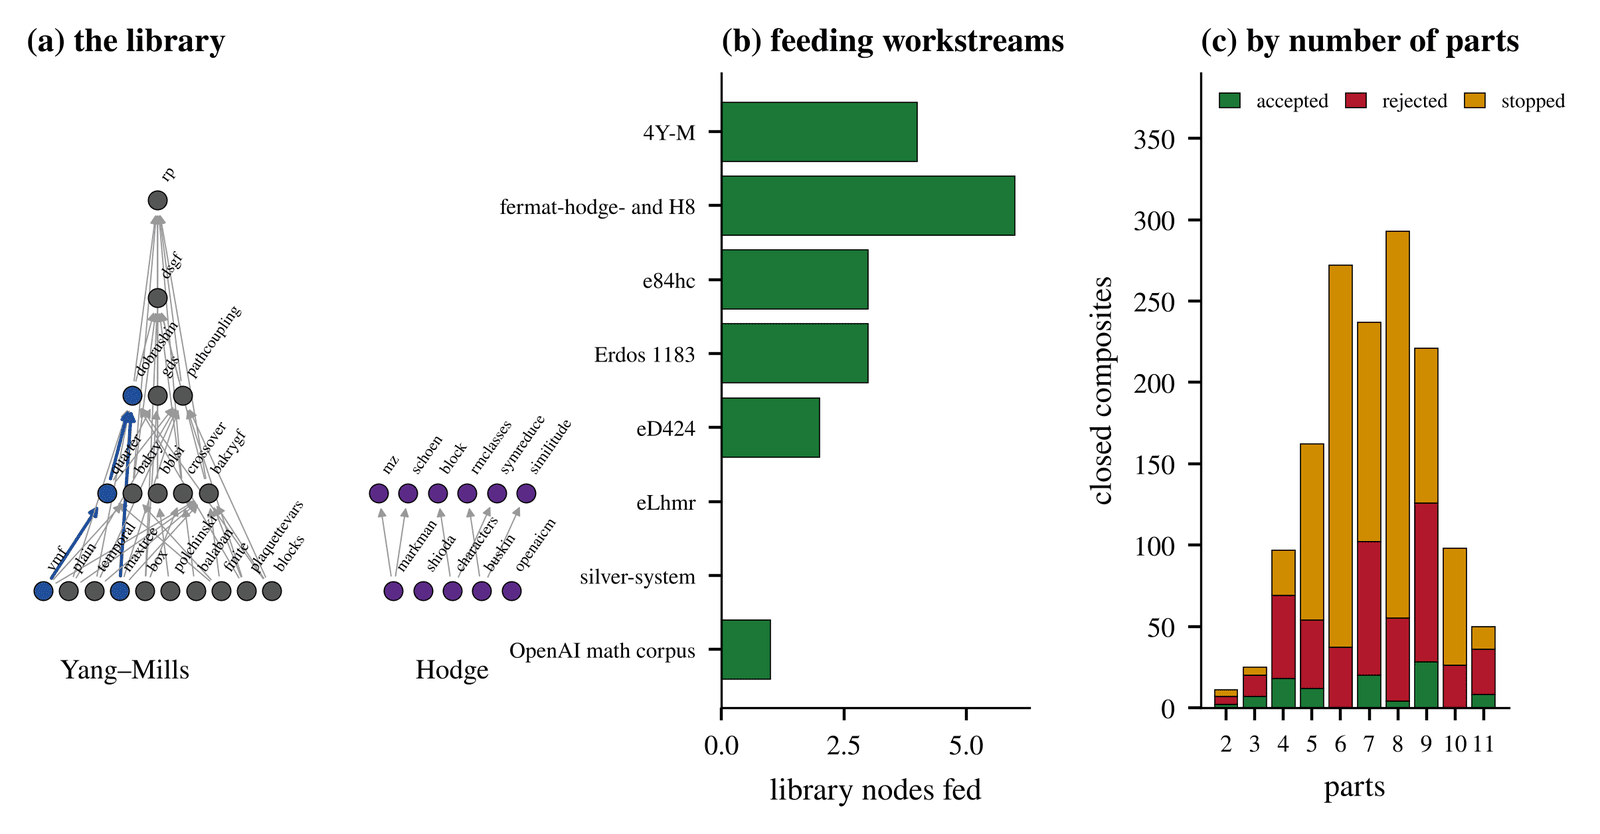
\includegraphics[width=0.98\textwidth]{figures/fig_graph}
\caption{The construction graph. (a) The library of the amplified round, with an arrow from $b$ to $a$ when $b$ can be fed into $a$, layered by the length of the longest chain of inputs; Yang--Mills nodes on the left, Hodge nodes on the right, and the four parents of the composite that proves $\beta_{W}<\frac13$ in blue. (b) The number of library nodes fed by each workstream. (c) Closed composites of the amplified library by number of parts and outcome.}
\label{fig:graph}
\end{figure*}

\subsection{Memory}\label{ssec:memory}

The memory study runs the whole package over the five libraries for $5$ rounds and $60$ seeds, with $8$ generations of $10$ crosses per round, in five arms: the full system (boosters, memory, retrieval, the committee of proposers); the full system without retrieval, which keeps the memory but does not let it steer; boosters alone; no boosters; and random pairing. Every arm without memory starts each round from the library and keeps only its synapse weights. The measured quantities are the distinct survivors after each round and the checks spent on them (Fig.~\ref{fig:memory}).

\begin{figure*}[t]
\centering
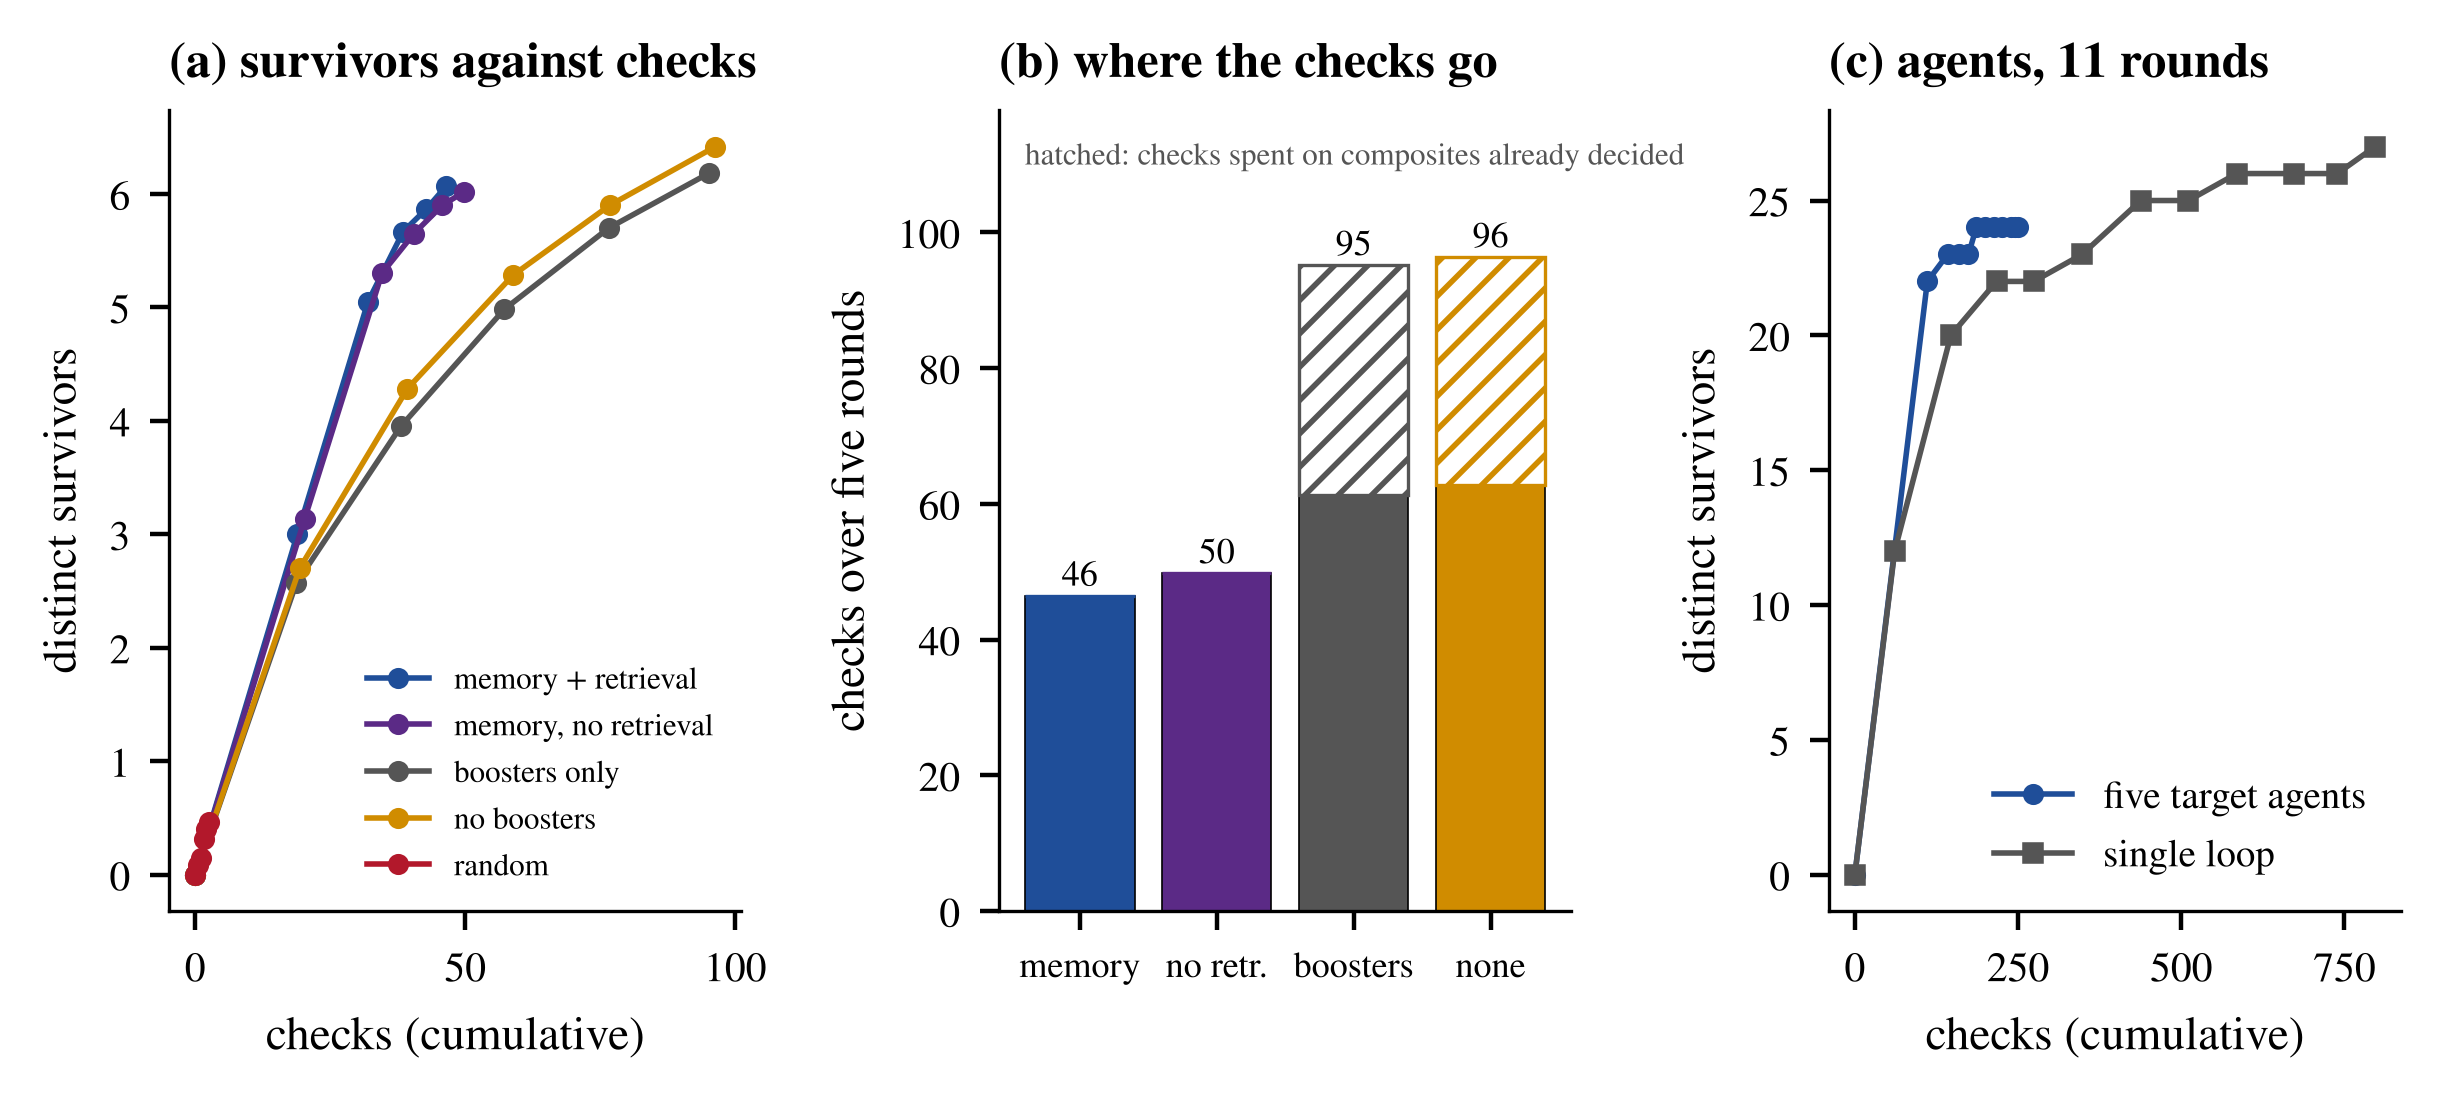
\includegraphics[width=0.98\textwidth]{figures/fig_memory}
\Description{Curves of distinct survivors against cumulative checks over five rounds, bars of checks with the part spent on already decided composites hatched, and five target agents against the single loop.}
\caption{Memory and agents. (a) Distinct survivors against cumulative checks over five rounds, mean of $60$ seeds; each marker is one round. (b) Checks over the five rounds; the hatched part is spent on composites that an earlier round of the same seed had already decided. (c) The five target agents against the single-loop control in the continuous loop, with the local model among the proposers; each marker is one round.}
\label{fig:memory}
\end{figure*}

\begin{table}[t]
\caption{The memory study: five rounds, $60$ seeds, means per seed. ``Repeated'' counts checks of composites decided in an earlier round.}
\label{tab:memory}
\centering
\footnotesize
\setlength{\tabcolsep}{3.5pt}
\begin{tabular}{@{}lrrrr@{}}
\toprule
Arm & Checks & Repeated & Survivors & Refuted \\
\midrule
full system & $46.4$ & $0.0$ & $6.07$ & $5.2$ \\
no retrieval & $49.8$ & $0.0$ & $6.02$ & $5.3$ \\
boosters only & $95.2$ & $33.9$ & $6.18$ & $10.6$ \\
no boosters & $96.3$ & $33.6$ & $6.42$ & $10.6$ \\
random & $2.5$ & $0.1$ & $0.47$ & $0.3$ \\
\bottomrule
\end{tabular}
\end{table}

Every arm except random pairing ends between $6.0$ and $6.4$ distinct survivors, because the five libraries hold that many checkable statements within reach of the crosses; all of them are known results. The arms differ in cost (Table~\ref{tab:memory}). With memory the system reaches the plateau with $46.4$ checks, against $95.2$ for boosters alone, and spends none on composites already decided; without memory a third of the checks after the first round are repeats. Retrieval steers the draw but changes little, $46.4$ checks against $49.8$: the saving comes from not checking a decided composite twice, which is the soundness bookkeeping of Section~\ref{sec:chains} applied across rounds. Memory therefore halves the cost of reaching what the libraries can reach, and it does not move the plateau.

\subsection{The channel and the agents}\label{ssec:agentsexp}

The channel study runs the five agents on one shared memory for $6$ rounds and $60$ seeds in three arms: the channel with the target weights, the target weights alone, and neither. The three arms spend $211.8$, $218.0$ and $216.8$ checks per seed over the six rounds, with standard errors below one check, and end with $24.05$, $24.15$ and $24.23$ distinct survivors. The channel saves three per cent of the checks, because a bundle that carries a failed cell halves the weight of its candidate, and it costs a tenth of a survivor for the same reason. In none of the $180$ runs does a survivor reach a target point. The channel delivers everything the engine holds, and what the engine holds are outputs of library constructions; no library holds the input that a target point needs (Section~\ref{ssec:whyhard}).

The continuous loop runs the five agents and, beside them, a single-loop control: one attack over all five libraries with boosters and no memory, $6$ generations of $40$ crosses per round. The agents use the channel, the target weights and the local model. After eleven rounds the agents hold $24$ distinct survivors for $250$ checks and the control $27$ for $797$ (Fig.~\ref{fig:memory}(c)). The agents reach $23$ survivors in the second round, for $142$ checks, and $24$ in the fifth; the control needs five rounds and $348$ checks to reach $23$ and passes the agents in the sixth round, still adding a known result every few rounds at about $70$ checks per round. No survivor of either reaches a target point. Agents are cheaper for the same reason as memory, since each agent skips what its slice of the store has decided, and they reach no further, since a target point needs an input that no library holds; the control's three extra survivors are known results that the agents' narrower libraries do not contain.

\subsection{The barrier and pattern matrix}\label{ssec:matrix}

The last experiment is done by hand and recorded in the package. For each blocking step, every pattern that broke a comparable barrier elsewhere is transferred, and the transferred statement, its needed input and the outcome are written as one cell: \emph{closes} when the pass line is crossed, \emph{partial} when a weaker statement follows or a new fact is computed, \emph{fails} when the needed input is false or unknown, with the reason. There are $38$ cells. None closes; $7$ are partial and $31$ fail. The partial cells are the forest gauge fixing and its ceiling, the box Dobrushin--Shlosman criterion as a finite check not yet run, size colourings and Theorem~\ref{thm:fvalues}, the forced arithmetic progressions in level colourings, the Kuga--Satake reduction of Varesco, the averaged Chowla theorem, and the grid search at $n=20$. The failures fall into three kinds: the input is known to be false (product colourings and m-sequence colourings for Erd\H{o}s problem 1183, plaquette variables, abelian duality for $\mathrm{SU}(2)$), the input is the open problem itself or another benchmark (motivated cycles, which are algebraic exactly when the standard conjecture holds; the inverse of $L$ as a Hodge class on $X\times X$), or the input needs a small parameter that is not small at the blocking step (Ba{\l}aban, Brydges--Yau, Kotecký--Preiss). The matrix is the content of the cells $\pi_{\mathrm{ch}}$ of \eqref{eq:channelprior} reads, so a pattern recorded as failing on a benchmark is drawn half as often there.

Two cells are new computations and one is a new negative result.

\begin{proposition}\label{prop:productrules}
Let $c_{1},c_{2}$ be level colourings of $2^{[a]}$ and $2^{[b]}$ attaining $f(a)$ and $f(b)$, and colour $S\subseteq[a+b]$ by $\phi(c_{1}(S\cap[a]),c_{2}(S\setminus[a]))$ for a Boolean function $\phi$ of two variables that depends on both. For $a=b=4$ the largest monochromatic sublattice has $16$ members when $\phi$ is exclusive or or its negation, $32$ for disjunction and $48$ for conjunction, against $f(4)+f(4)=6$.
\end{proposition}

The grid search of Lemma~\ref{lem:levelposet}, run with two blocks, computes these values. They show why subadditivity $f(a+b)\le f(a)+f(b)+C$ cannot come from such products: a monochromatic sublattice of the product projects to sublattices of the factors, but the colour of a product point is a function of both factors, so the projections need not be monochromatic, and the product lattice of two chains is a grid with $(a+1)(b+1)$ members.

At $n=20$ the grid colourings with two blocks of sizes $18$ and $2$, $57$ grid points, were searched by simulated annealing on the number of pairs (colour, base point) from which a monochromatic sublattice of $12$ members is reachable. Of $24$ restarts, $16$ end with exactly one such pair and none with zero; every colouring obtained from the best one by changing one or two grid points keeps a bad pair. Refining the best colouring to three blocks of sizes $(16,2,2)$ and $(17,1,2)$ and annealing again, four restarts, also ends at one bad pair. None of the runs reaches zero, and none can: by the twenty-level window cited in Theorem~\ref{thm:fvalues}, every colouring of $2^{[20]}$ has a monochromatic sublattice of $12$ members.

The colourings with the shortest monochromatic progressions known come from finite fields, and they were the natural candidates for an answer to Question~9.3. They fail.

\begin{proposition}\label{prop:mseq}
Let $\alpha$ be a primitive element of $\mathbb{F}_{2^{p}}$, $\beta\neq0$, $n\le2^{p}-2$, and colour $S\subseteq[n]$ by $\mathrm{Tr}(\beta\alpha^{|S|})$. \textup{(i)} If $p$ is prime, every monochromatic sublattice isomorphic to a Boolean lattice has at most $2^{p-1}$ members. \textup{(ii)} If $\alpha^{e}=1+\alpha^{d}$ and $\mathrm{Tr}(\beta\alpha^{t+jd})=0$ for $0\le j\le k$, with $t+k\max(d,e)\le n$, there is a monochromatic sublattice with $3^{k}$ members. If $\alpha$ is a root of the trinomial $x^{p}+x+1$ and $n=2^{p}-2$, a suitable $\beta$ allows $d=1$, $e=p$, $t=0$ and $k=p-2$, which gives $3^{p-2}=\frac19(n+2)^{\log_{2}3}$ members.
\end{proposition}

\begin{proof}
A Boolean sublattice of rank $k$ is $J(P)$ for an antichain $P=\{1,\dots,k\}$ with weights $w_{i}$ and base $t$, and its members have colours $\mathrm{Tr}(\beta x)$ for $x$ in $X=\{\alpha^{t}\prod_{i\in I}\alpha^{w_{i}}\}$, whose span is $\alpha^{t}\prod_{i}\mathrm{span}\{1,\alpha^{w_{i}}\}$; each factor is a plane, since $1\le w_{i}\le2^{p}-2$. For prime $p$ the field $\mathbb{F}_{2^{p}}$ has no subfield other than $\mathbb{F}_{2}$ and itself, so the theorem of Hou, Leung and Xiang \cite{HLX02} gives $\dim(UV)\ge\min(p,\dim U+\dim V-1)$ for nonzero subspaces $U,V$, and the span has dimension at least $\min(p,k+1)$. Colour $0$ puts it in a hyperplane, so $k\le p-2$. For colour $1$ the differences $\alpha^{t}(1+\alpha^{w_{j}})\prod_{i\in I}\alpha^{w_{i}}$, $I\not\ni j$, have trace $0$ and span a product of $k-1$ planes times one element, so $k\le p-1$. This is (i). For (ii) take $k$ disjoint chains, each with ranks $0$, $d$ and $e$. Their down-sets have ranks $t+ad+be$ with $a+b\le k$, and $\alpha^{t+ad+be}=\alpha^{t}(\alpha^{d})^{a}(1+\alpha^{d})^{b}$ lies in the span of $\alpha^{t},\alpha^{t+d},\dots,\alpha^{t+kd}$, so every member has trace $0$, and $t+k\max(d,e)\le n$ keeps all ranks in range. The sublattice has $3^{k}$ members. For the trinomial, $\alpha^{p}=1+\alpha$, and the condition asks for a run of $k+1$ zeros in the $m$-sequence $\mathrm{Tr}(\beta\alpha^{i})$; each period has a run of $p-1$ zeros, choosing $\beta$ moves it to $t=0$, and $(p-2)p\le2^{p}-2$.
\end{proof}

For the colourings defined by $x^{5}+x^{2}+1$, $x^{6}+x+1$ and $x^{7}+x+1$ at $n=2^{p}-2$, the largest sublattices of the form (ii) have $27$, $81$ and $243$ members, or $0.84$, $1.27$ and $1.90$ times $n+2$, with $(d,e)=(2,5)$, $(1,6)$ and $(1,7)$. The linearity that keeps the progressions of both classes at length $p-1$ turns every progression whose difference has a small partner $e$ into a triangle of ranks, so an answer to Question~9.3 by level colourings needs classes that avoid both.


\section{Construction mode}\label{sec:construct}

The crossing network combines what its library holds, and on every open step of the five benchmarks the library holds nothing that combines into the next object. Construction mode is the part of the engine that writes a new object down. It builds the object together with the argument for what the object forces, and it keeps the object only after the gate of Section~\ref{ssec:construct}, which checks it again from scratch. This section tests it on a problem whose answer people found, so that a success can be recognised, and then asks whether towers of builders find answers with fewer checks.

\subsection{Steinberg's problem from its rules}\label{ssec:steinberg}

Steinberg conjectured in 1976 that every planar graph with no cycle of length $4$ or $5$ is $3$-colourable \cite{Ste93,CHK17}, and Erd\H{o}s asked for the least $k$ such that every planar graph with no cycle of length $4$ to $k$ is $3$-colourable \cite{BGR05,CHK17}. Borodin, Glebov, Raspaud and Salavatipour proved that $k\le7$ \cite{BGR05}. Cohen-Addad, Hebdige, Kr\'al', Li and Salgado refuted Steinberg's conjecture in 2016, so $k\ge6$ \cite{CHK17}; whether $k=6$ or $k=7$ is open. Their construction has three steps. A \emph{gadget} $G_{1}$ on $15$ vertices has three contacts on one face, at distances $3$, $3$ and $4$, and no $3$-colouring gives the three contacts one colour; three copies of $G_{1}$ and a triangle make a gadget $G_{2}$ on $42$ vertices whose contacts are pairwise at distance $4$; and four copies of $G_{2}$ in a planar frame give a graph with no cycle of length $4$ or $5$ that is not $3$-colourable. The step that needs invention is the first: once a gadget of the right profile exists, the second and third steps are assemblies.

The engine was given the rules (planar with the contacts on one face, no cycle of length $4$ or $5$, the contact distances, and the requirement that no $3$-colouring gives the contacts one colour) and nothing about the answer. Table~\ref{tab:steinberg} lists the methods and what each found.

\begin{table*}[t]
\caption{Construction mode on Steinberg's problem. Every gadget in the table passed the gate: planarity with the contacts on one face, every cycle length up to $7$, the contact distances, and the forcing property by backtracking and by three satisfiability solvers. ``Isomorphic'' means isomorphic to the gadget of \cite{CHK17} with the contacts matched.}
\label{tab:steinberg}
\centering
\footnotesize
\setlength{\tabcolsep}{4pt}
\begin{tabular}{@{}p{0.24\textwidth}p{0.30\textwidth}p{0.40\textwidth}@{}}
\toprule
\rr Target & \rr Method & \rr Outcome \\
\midrule
\rr gadget, distances $3,3,4$ & \rr random planar frames filled with library gadgets & \rr none in $2.45$ million frames \\
\rr the same & \rr goal-directed builder, rules only & \rr $15$ vertices, $23$ edges, isomorphic to $G_{1}$; try $116$, $11$\,s \\
\rr the same & \rr exists-forall search over two-page book embeddings & \rr a $15$-vertex, $23$-edge gadget in $2.5$\,s ($1{,}172$ rounds) \\
\rr gadget, distances all $\ge4$ & \rr builder, rules only & \rr nothing: from contacts this far apart no rule applies \\
\rr the same & \rr builder with the rebuilt $G_{1}$ and a triangle gadget as lemmas & \rr $42$ vertices, $72$ edges, isomorphic to $G_{2}$, on two seeds (tries $13$ and $9$); on a third seed $48$ vertices with distances $5,4,5$ (try $8$, $3.5$\,s) \\
\rr the whole graph & \rr assembly of \cite{CHK17} on the rebuilt $G_{1}$ & \rr $166$ vertices and $300$ edges, planar, cycles of length at most $6$ only of lengths $3$ and $6$, not $3$-colourable by CaDiCaL, Glucose and MiniSat \\
\rr Erd\H{o}s's question: no cycle of length $4$, $5$ or $6$ & \rr all of the above & \rr nothing; open \\
\bottomrule
\end{tabular}
\end{table*}

\emph{The builder.} The builder starts from three contacts that share a colour and adds a vertex or an edge only when a forcing rule uses it: a vertex joined to two vertices of the shared colour receives one of the two other colours, a vertex joined to two vertices of different colours other than the shared one is forced, and two adjacent vertices forced alike close the argument. After each move it applies the cheap tests of the cascade (forbidden cycles, distances, planarity with the contacts on one face) and only then one exact satisfiability check; it stops when the check says the contacts can no longer share a colour, and then deletes vertices while the property holds. On the profile $3,3,4$ it found on its $116$th try, after $11$ seconds, a gadget on $15$ vertices and $23$ edges that is isomorphic to $G_{1}$ with its contacts, and in the same run a gadget on $18$ vertices with distances $3,3,5$.

\emph{Why the rules stop at distance four.} With no cycle of length $4$, the neighbours of one contact that are not of the shared colour form a matching; a vertex joined to both ends of an edge of that matching closes a $4$-cycle, and an edge between the neighbourhoods of two contacts puts them at distance $3$. So from three contacts pairwise at distance at least $4$ no forward rule derives anything, and the long distances of $G_{2}$ come from using $G_{1}$ as a lemma, which is a case split, not a forward step. The engine therefore keeps every gadget it finds as a lemma: a library gadget whose two contacts are forced to the shared colour forces its third contact to differ, and the builder may add such a copy as one move. With the rebuilt $G_{1}$ and the triangle gadget as lemmas it built a gadget isomorphic to $G_{2}$ on two seeds.

\emph{The exact search.} The second method searches for a graph and a proof together: an exists-forall loop proposes a graph on $n$ vertices from a satisfiability instance and refutes it with a colouring, which becomes a clause. Requiring the graph with one extra vertex joined to the contacts to have a two-page book embedding along a fixed spine makes every candidate planar with the contacts on one face, so the crossing rule is a fixed list of clauses and no Kuratowski cuts are needed. On Steinberg's profile it found a $15$-vertex gadget in $2.5$ seconds, where the same loop with lazy Kuratowski cuts had not finished this size after $30$ minutes. A ``none'' from this search covers only the graphs that are two-page along the spines tried.

\emph{Erd\H{o}s's question.} The same assemblies reduce the question to one gadget: a gadget with no cycle of length $4$, $5$ or $6$, planar with the contacts on one face, forcing the contacts not all equal, with distances $3$, $3$ and at least $5$, would give through $G_{2}$ and the frame a planar graph with no cycle of length $4$, $5$ or $6$ that is not $3$-colourable, and so $k=7$. The book search found no such gadget on $16$ vertices along the spines tried, a search that treats each triangle gadget as one node found none up to $13$ nodes, and the builder with the lemmas of this case found none. A gadget built by hand from triangle gadgets has every property except planarity, on $24$ vertices with distances $3,3,6$; once three of its vertices are placed, one contact and the other two lie on different faces, and no later gadget can join the two sides. The wall for $k=6$ is the planar arrangement of the forcing argument, not the forcing argument.

The calibration therefore passes in the sense that was fixed before it: the engine invented the gadget that people invented, from the rules, and assembled the counterexample from it. It is a rediscovery of a published construction, and on the question that remains open it found nothing.

\subsection{Towers at equal cost}\label{ssec:towerbench}

\TOWERBENCH{}

\section{One problem only: the Hodge round}\label{sec:hodgeround}

The runs of Section~\ref{sec:experiments} spread the network over five problems. This section points the whole of it at one, the Hodge conjecture in the form of \cite{BB26c}: the conjecture is equivalent to two statements about abelian varieties, (F2), that every Hodge class on an abelian variety outside the part $R(Y)$ reached from the known constructions is algebraic, and (F3$'$), that on every smooth projective variety the Hodge classes are those coming from abelian varieties, $\mathrm{Hdg}^{p}=\mathrm{Ab}^{p}$. The paper proves that the locus on which either statement holds is dense in every family and is either everything or meagre, and it builds for each statement the object that would decide it next and proves at which step the construction stops. Those stopping points are the five target points of Table~\ref{tab:hodgetargets}. The question for the network is whether, with every result of \cite{BB26c}, of the companion paper on Weil classes \cite{BMB26b} and of the literature in its library, and with the fourteen external sources of Section~\ref{ssec:hodgesources}, it produces one object that passes one target point. The measured quantity is the gap of Section~\ref{ssec:gapnumbers}: for each target point the number of open steps between the best checked composite and the point, together with the counts of composites checked, rejected and stopped. Everything in this section was fixed before the runs except the numbers.

\begin{table*}[t]
\caption{The five target points of the Hodge round, from \cite{BB26c}. Each is the object that paper needs next and could not build; ``open steps'' is the depth of the deepest open step in the library's route to the point, the gap of Fig.~\ref{fig:hodgerounds}(c). None is reached.}
\label{tab:hodgetargets}
\centering
\footnotesize
\setlength{\tabcolsep}{4pt}
\begin{tabular}{@{}p{0.12\textwidth}p{0.42\textwidth}p{0.30\textwidth}p{0.08\textwidth}@{}}
\toprule
\rr target & \rr object that passes it & \rr where \cite{BB26c} stops & \rr open steps \\
\midrule
\rr F2.lift & \rr for one polarised abelian scheme $A\to S$ with a flat Hodge class $\xi$ algebraic at a CM point $c$, a semiregular object at $c$ with Chern character $\xi_{c}$; then $\xi$ is algebraic on all of $S$ & \rr the CM point exists in every family; the semiregular object at it does not & \rr 3 \\
\rr F2.E06 & \rr a convolution $E$ of the pieces $O_{Z_{\zeta}}\otimes L^{k}[s]$, $L^{l}[t]$ on $E_{0}^{6}$, $E_{0}=\mathbf{C}/\mathbf{Z}[i]$, with $\mathrm{ch}(E)$ of polarised shape and $\dim\mathrm{Ext}^{2}(E,E)=57$ & \rr the $35$ pieces of its Proposition on separation give $\dim\mathrm{Ext}^{2}\ge2605$; four configurations are left open & \rr 2 \\
\rr F2.link & \rr one algebraic class $\xi\in\mathrm{Hom}_{\mathrm{Hdg}}(T_{X}(-1),T_{Z})$ on $X\times X\times Z_{K}$ for a Mumford fourfold $X$ whose cubic field $F$ contains no imaginary quadratic field & \rr $\mathrm{Hom}(X,Z_{K})=0$; the class is a Hodge class on a CM sixfold and nothing produces it & \rr 1 \\
\rr F3.cubic & \rr an algebraic correspondence of $S_{\lambda}$ (Picard number $13$, transcendental rank $9$) acting on $T(S_{\lambda})$ through the cubic field $F$, with $(F,D)$ not $(\mathbf{Q}(\zeta_{7})^{+},D_{\infty})$ or $(\mathbf{Q}(\zeta_{9})^{+},D_{\infty})$ & \rr finite groups reach only $\mathbf{Q}(\zeta_{7})^{+}$ and $\mathbf{Q}(\zeta_{9})^{+}$; a self-map $f$ with $f^{2}=n$ in $F$ forces $f\in\mathbf{Q}$ & \rr 1 \\
\rr F3.sqrt & \rr a family of K3 surfaces with real multiplication by $\mathbf{Q}(\sqrt{10})$ or $\mathbf{Q}(\sqrt{14})$ on which a chain of symplectic quotients or an isogeny of elliptic surfaces starts & \rr the chain theorem gives $\sqrt6$ and the Fricke cases; no family starts the chain for $\sqrt{10}$, $\sqrt{14}$ & \rr 1 \\
\bottomrule
\end{tabular}
\end{table*}

\subsection{Library, agents and rounds}\label{ssec:hodgerun}

The library for this round has $76$ typed constructions: the $19$ results of \cite{BB26c} that bear on the target points; $9$ of \cite{BMB26b}, namely Markman's theorem for trivial discriminant, the Weil tori, the convolutions on $E_{0}^{6}$ and on $E_{0}^{8}$, the quartic rank, the abelian covers, Schoen's product, the Vandermonde intersections and the escape theorem; $34$ results of the literature from Deligne to Markman's recent work, among them one unrefereed claim, the family of preprints in \cite{OAI26b} that asserts the Hodge conjecture for abelian varieties of CM type and for products of K3 surfaces, which enters as a hypothesis and never as a result; two counts computed for this round (Section~\ref{ssec:hodgecount}); six moves that change the variety (blow-up at a CM point, degeneration to a CM fibre, Kuga--Satake passage, fibration, Hilbert scheme, isogeny cover); and six open conjectures from the OpenConjecture collection (Section~\ref{ssec:hodgesources}), which the refuter treats as hypotheses, so that a composite resting on one is recorded as conditional and stopped. One agent sits on each target point. In a \emph{steady} round each agent runs six generations of ten pairings, with the refuter and the memory of Section~\ref{ssec:memory}; in a \emph{burst} each agent runs ten generations of forty pairings and the round then checks three hundred random chains of three to six constructions, pruned by the same refuter. Every checked composite is recorded with its verdict and its reason, so that no later round checks it again.

Rounds $1$ to $11$ were steady and round $12$ was a burst. Fig.~\ref{fig:hodgerounds} shows the run. The memory records $78$ checked composites in the first round, $29$ in the second, and between $7$ and $16$ in each of the next eight, as the combinations of the library are used up; round $11$, run after the two counts and the moves had entered the library, checked $35$. In all $230$ composites were checked in the eleven steady rounds, $22$ survived, and every survivor is a known result: the reduction to (F2) and (F3$'$), the propagation theorem, the density of CM points, Markman's theorem and the cases it covers. No composite reaches a target point, and the gap of every target point is the same after round $11$ as after round $1$: three open steps for F2.lift, two for F2.E06 and one for each of the other three.

Round $12$ had a time limit of $7000$ seconds. It committed $29$ checked composites to the memory in its first $98$ minutes and was stopped at the limit before it wrote its summary and before the long chains began. None of the $29$ survived. Twenty-four were stopped because they rest on an open conjecture used as a hypothesis, the derived form of the Hodge conjecture or a statement on generic Hodge classes from the OpenConjecture entries; three stopped at the count on $E_{0}^{6}$, one at the semiregular object of F2.lift, and one was rejected. Most of the time of the round went into the channel, which brought $58{,}872$ records of the memory to the proposers, against $11{,}558$ in round $11$ and between $1{,}546$ and $4{,}108$ in each earlier round. The burst therefore multiplies the cost of a round and moves the search toward composites that assume what they need; it does not change the gap. A wider search of the same library does not move a flat line at the depth of the first open step, because that step is not a combination of what the library holds.

\begin{figure*}[t]
\centering
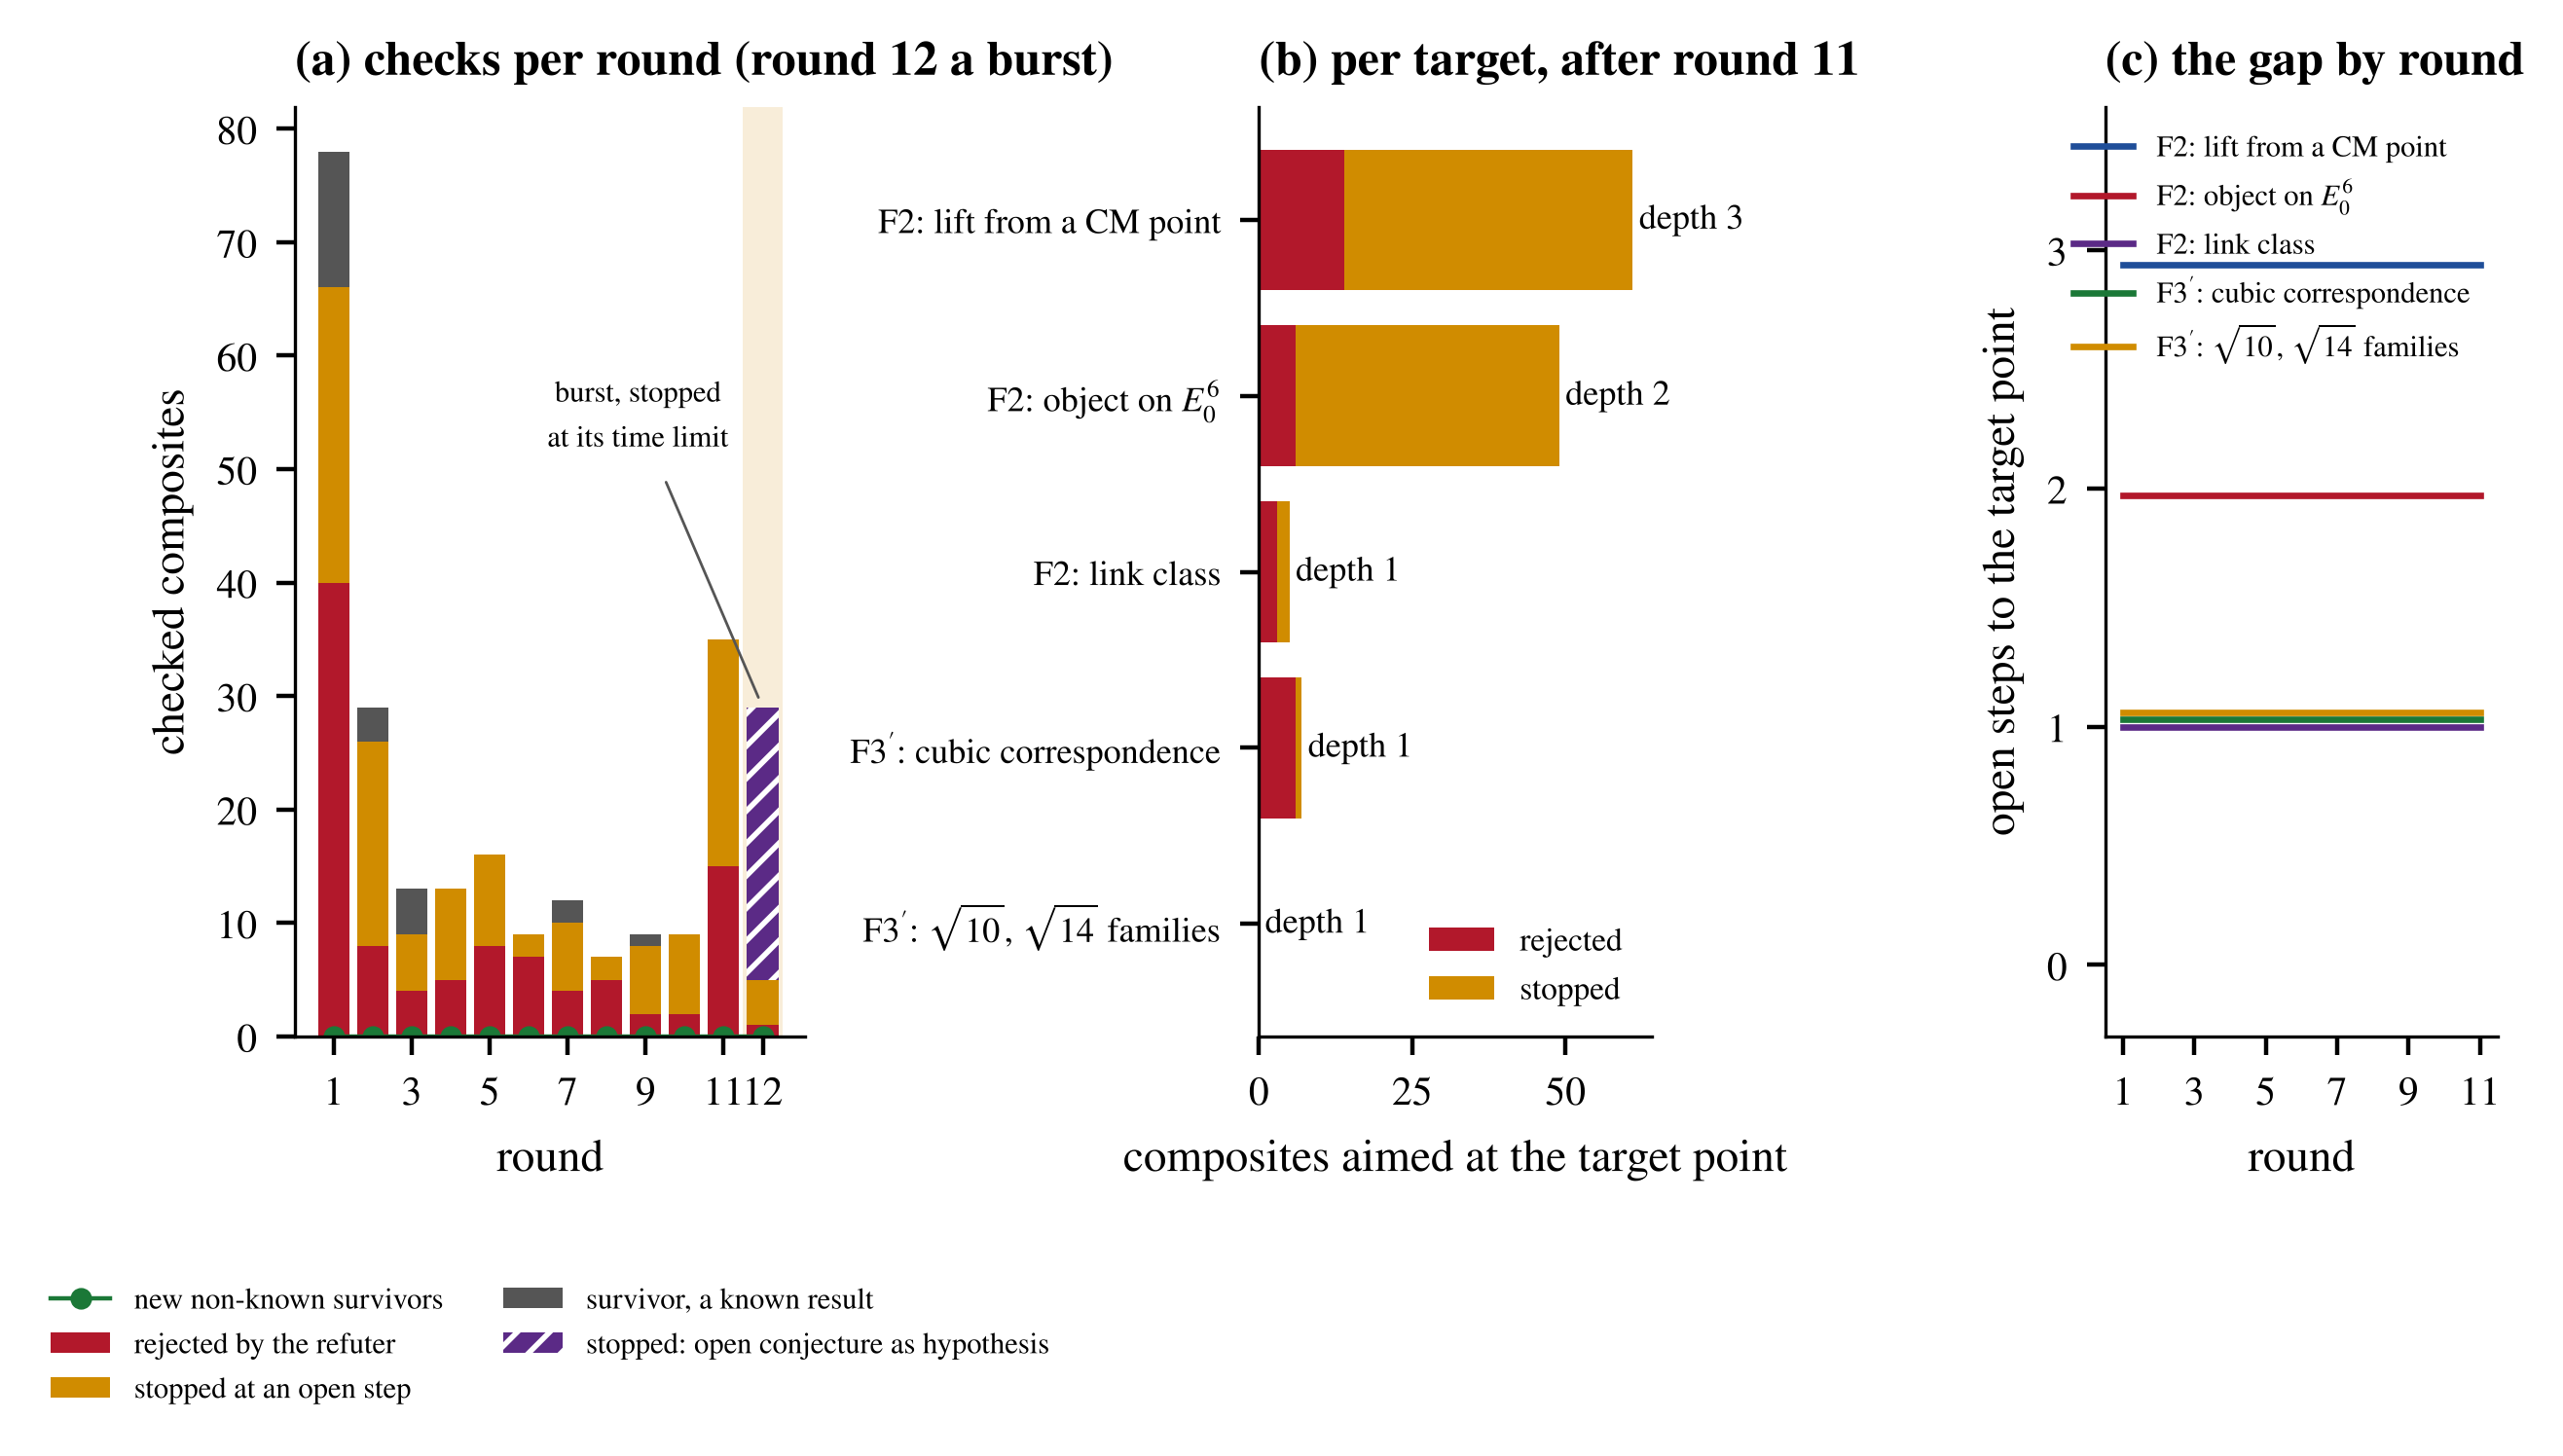
\includegraphics[width=0.98\textwidth]{figures/fig_hodgerounds}
\Description{Stacked bars of checked composites per round of the Hodge-only run: rejected, stopped at an open step, and survivors.}
\caption{The Hodge-only run. (a) Checked composites per round, from the memory: rejected by the refuter, stopped at an open step, and survivors, all of them known results; the green line, the survivors that are more than a known result, is zero in every round. Round $12$ (shaded) is the burst, stopped at its time limit; its hatched part rests on an open conjecture used as a hypothesis. (b) The composites aimed at each target point over rounds $1$ to $11$, with the depth of the gap after round $11$. (c) The gap of each target point by round: the number of open steps between the best checked composite and the point. It does not move.}
\label{fig:hodgerounds}
\end{figure*}

\subsection{Counting on \texorpdfstring{$E_{0}^{6}$}{E0\textasciicircum 6}}\label{ssec:hodgecount}

The target F2.E06 is the one that a finite computation can decide, and \cite{BB26c} leaves four configurations open after its $35$ pieces: (a) four or more line bundles, (b) one sheaf at two shifts, (c) one threefold at several twists, (d) two threefolds at the same shift meeting along an abelian surface. For a convolution $E$ of pieces $F_{a}$ the complex $\mathrm{Ext}^{\bullet}(E,E)$ is filtered by the blocks $\mathrm{Ext}^{k}(F_{a},F_{b})$ with total degree $k+s_{b}-s_{a}$, and $\dim\mathrm{Ext}^{2}(E,E)$ is at least the number of degree-two blocks that no differential reaches or leaves: a block $\mathrm{Ext}^{2}(F_{a},F_{b})$ is \emph{isolated} when no degree-one block maps to it along a chain of pieces and it maps to no degree-three block, and a bound that counts only isolated blocks is conservative, since a non-exact block can only add edges. The Ext groups of the pieces are the tables of \cite{BB26c} for $K=\mathbf{Q}(i)$, with $\chi_{Z_{\zeta}}=8$ and the groups between threefolds meeting along an abelian variety of dimension $d$ in $\prod_{j}\lvert\zeta_{j}-\zeta_{j}'\rvert^{2}$ components. We computed, for every polarised configuration of each family in a window of twists $1$ to $4$ and shifts $-3$ to $3$, the sums $C^{1},C^{2},C^{3}$ of the block dimensions by total degree, the Euler characteristic $C^{2}-C^{1}-C^{3}$, the isolated blocks, and a restricted Euler bound that removes the blocks that cannot interact. Fig.~\ref{fig:hodgepieces} shows the pieces of the least-bound configuration of family (a) and its block matrices; Fig.~\ref{fig:hodgebounds} shows the bounds over the families.

\begin{figure*}[p]
\centering
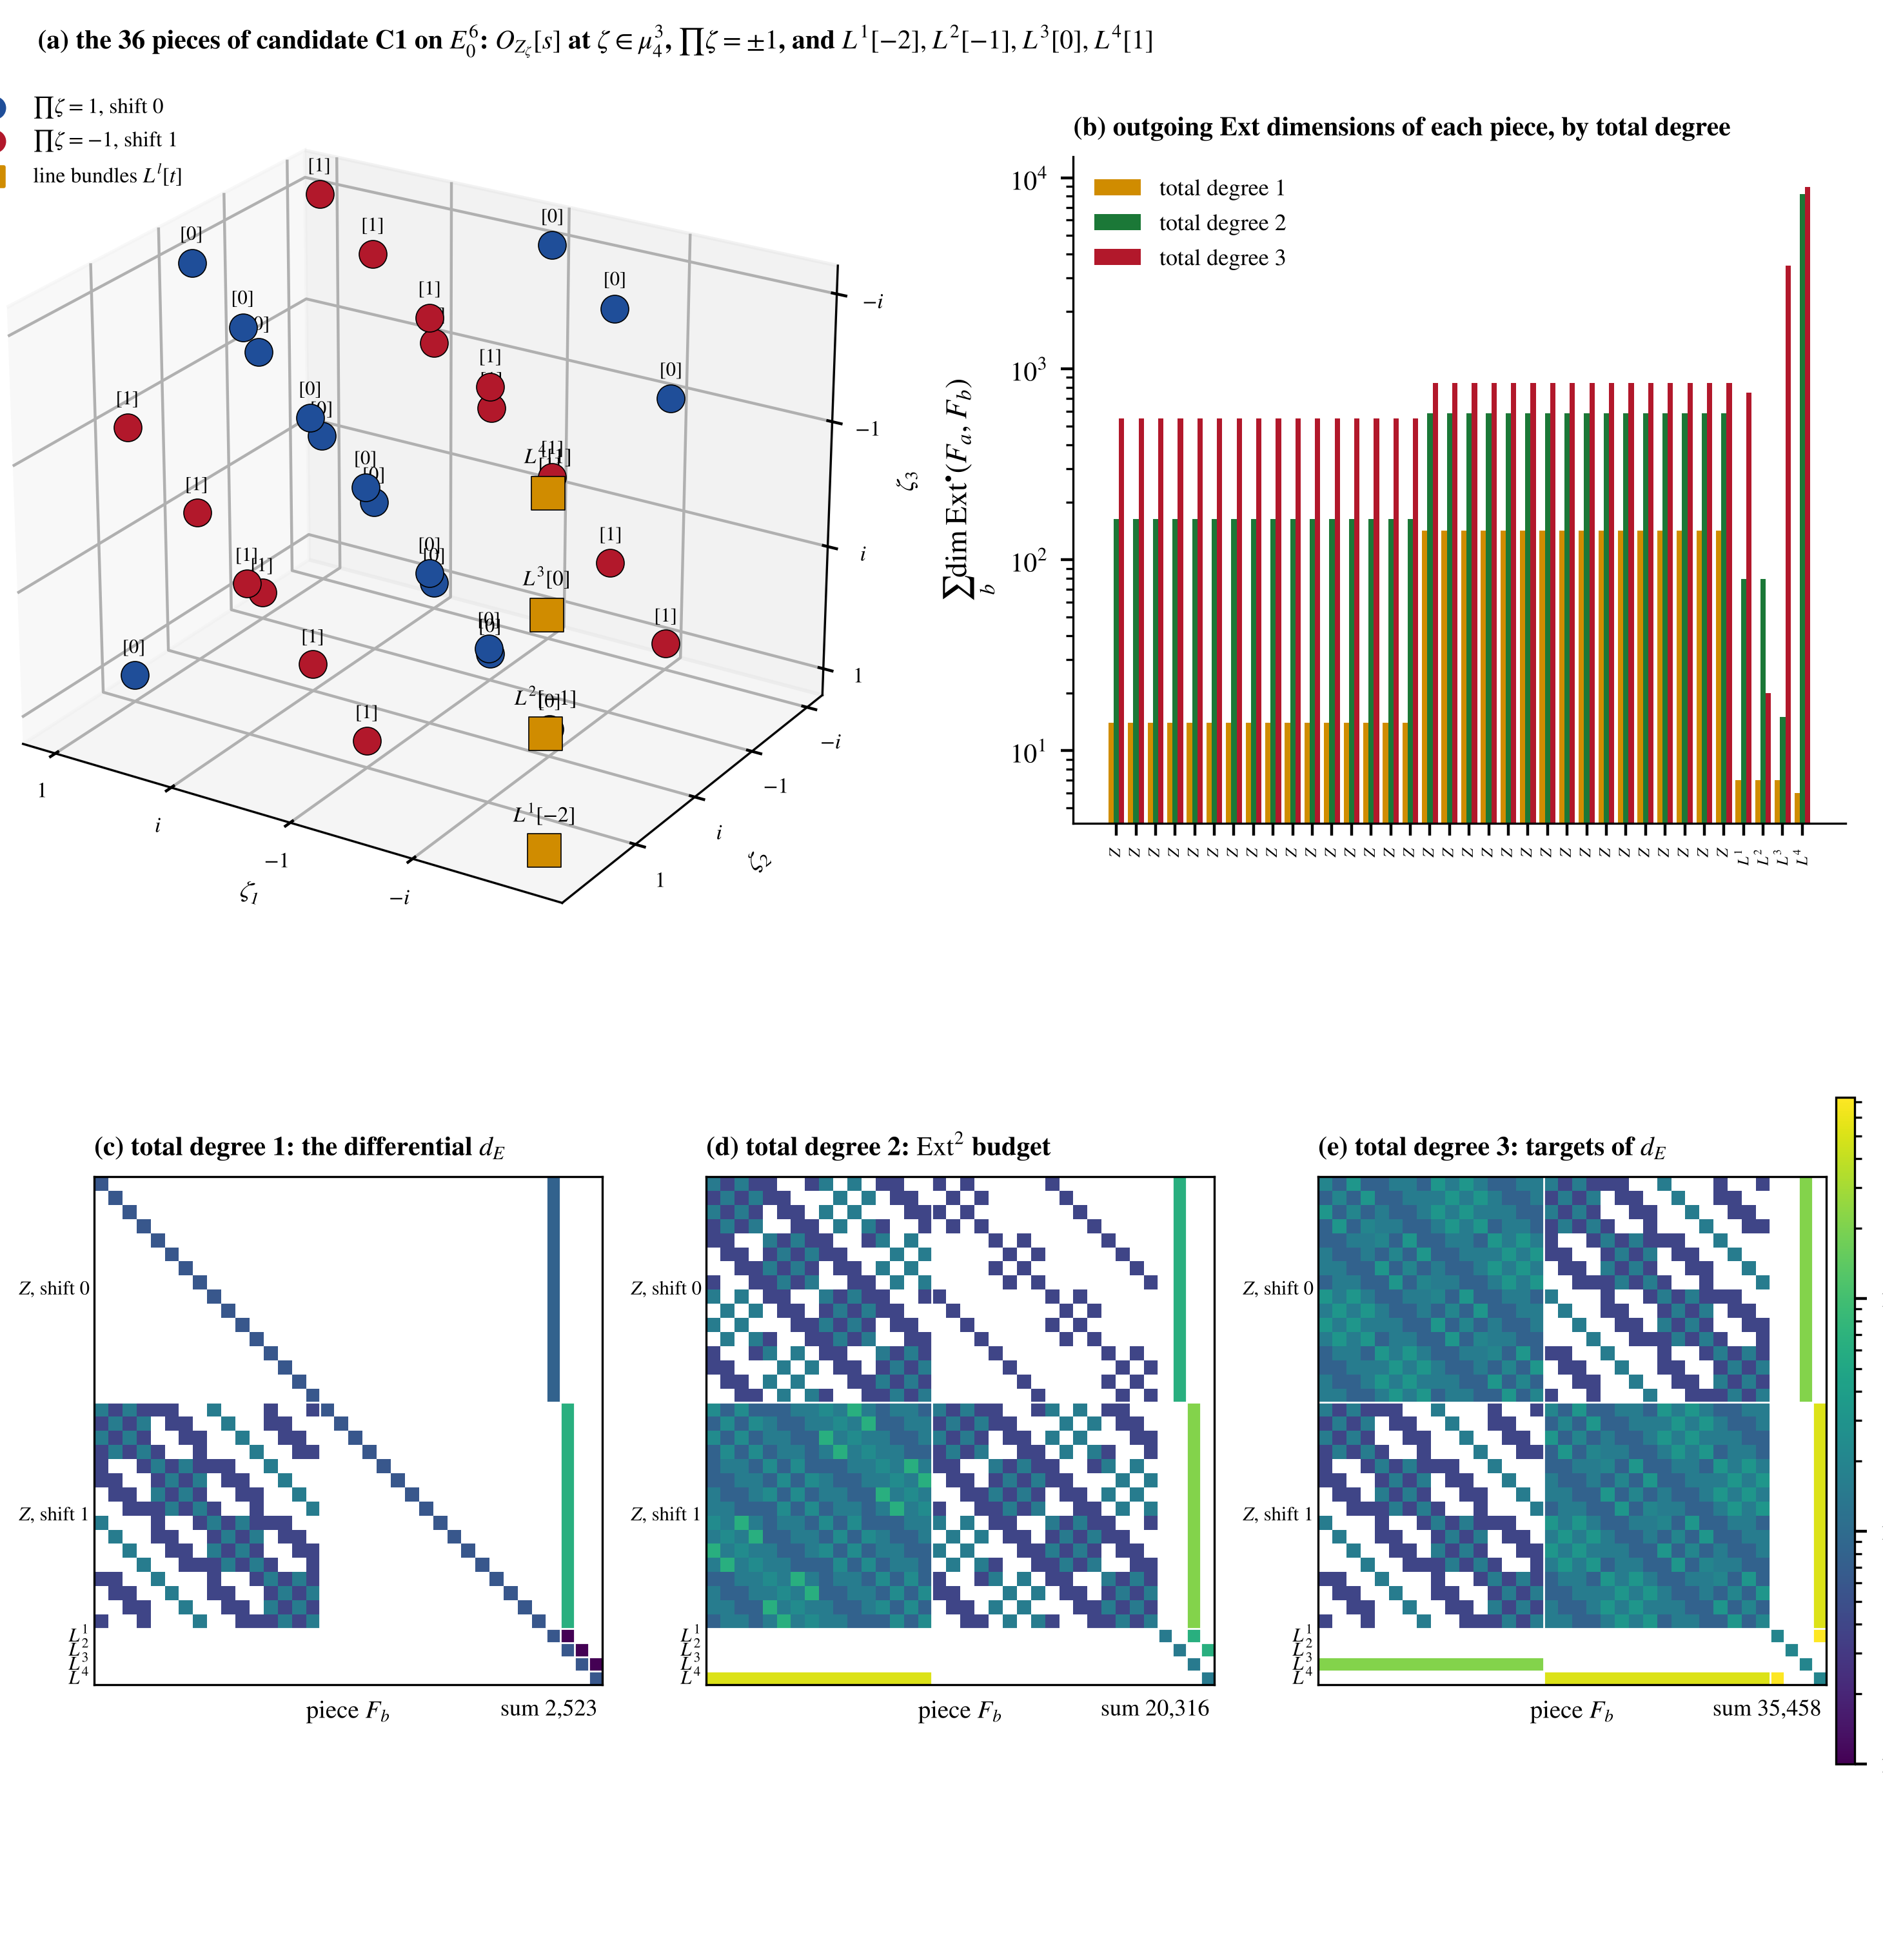
\includegraphics[width=0.98\textwidth,height=0.78\textheight,keepaspectratio]{figures/fig_hodgepieces}
\Description{Diagram of the thirty-two threefold pieces of candidate C1 on the sixfold and the blocks of their Ext groups.}
\caption{The pieces of candidate C1 on $E_{0}^{6}$ and their Ext blocks. (a) The $32$ threefold pieces $O_{Z_{\zeta}}[s]$ at the characters $\zeta\in\mu_{4}^{3}$ with $\prod\zeta=\pm1$, the sign fixing the shift, and the four line bundles $L^{1}[-2]$, $L^{2}[-1]$, $L^{3}[0]$, $L^{4}[1]$ of the least-bound configuration of family (a). (b) For each piece, the sum of the dimensions of the Ext groups to all pieces, by total degree. (c)--(e) The block matrices by total degree: the degree-one blocks carry the differential $d_{E}$, the degree-two blocks are the budget from which $\mathrm{Ext}^{2}(E,E)$ is cut, and the degree-three blocks are the targets of $d_{E}$ on degree two; the white lines separate the two parity classes of threefolds and the line bundles. Every degree-two block of this configuration is reached or leaves, so the counting bound is $0$ and the rank of the sixfold product decides.}
\label{fig:hodgepieces}
\end{figure*}

\begin{figure*}[t]
\centering
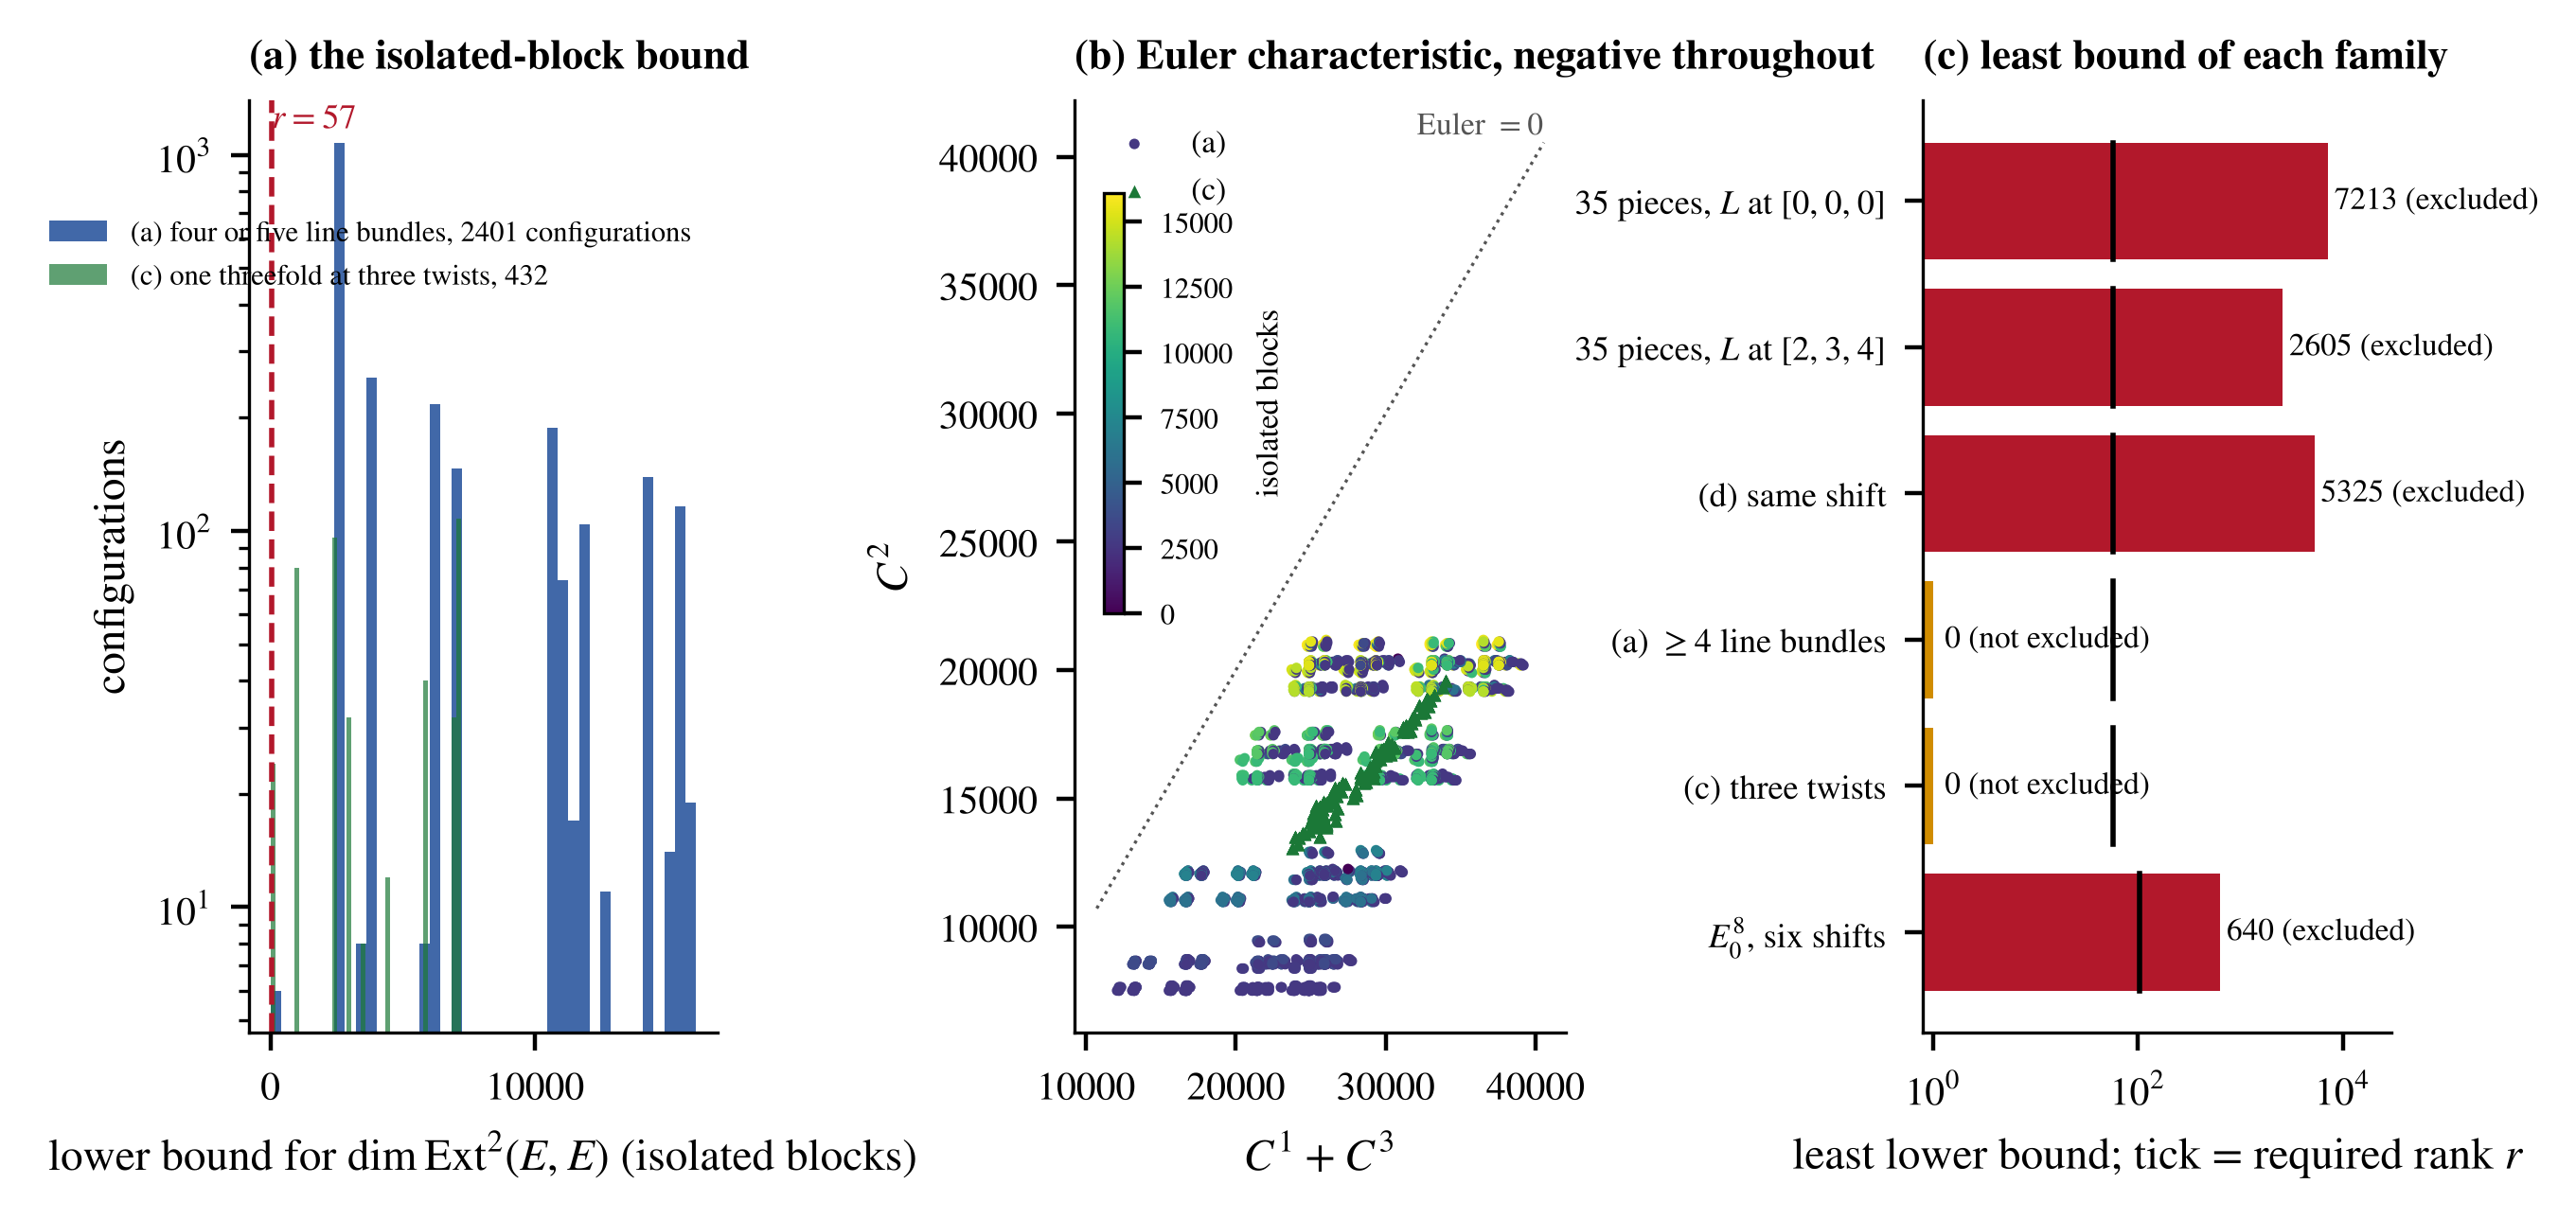
\includegraphics[width=0.98\textwidth]{figures/fig_hodgebounds}
\Description{Histograms of the isolated-block lower bound for the dimension of Ext squared over polarised configurations against the required rank 57, a scatter of Euler-characteristic terms, and the least bound of each family.}
\caption{Counting on $E_{0}^{6}$. (a) The isolated-block lower bound for $\dim\mathrm{Ext}^{2}(E,E)$ over the $2401$ polarised configurations of family (a) and the $432$ of family (c), against the required rank $r=57$. (b) $C^{2}$ against $C^{1}+C^{3}$ for the same configurations: the Euler characteristic is negative everywhere, so no configuration is excluded by it. (c) The least bound of each family against the rank it must meet: the $35$ pieces and family (d) are excluded, families (a) and (c) are not; the row for $E_{0}^{8}$ is the bound of \cite{BMB26b} within six shifts.}
\label{fig:hodgebounds}
\end{figure*}

The results are these. The $35$ pieces of \cite{BB26c} with the three line bundles at shifts $(0,0,0)$, $(2,3,4)$ or $(-3,-2,-1)$ have at least $7213$, $2605$ and $2605$ isolated degree-two blocks, so $\dim\mathrm{Ext}^{2}\ge2605>57$, in agreement with the bound $2560$ of \cite{BMB26b} for its line-bundle model. Family (d), two threefolds at the same shift meeting along a surface, has six polarised configurations in the window and the least bound is $5325$: it is excluded. Family (b) has no polarised configuration in the window. Family (a) has $2401$ polarised configurations, and for the four line bundles $L^{1}[-2],L^{2}[-1],L^{3}[0],L^{4}[1]$ the isolated blocks are $0$ and the Euler characteristic is $-17665$; family (c) has $432$, and for one threefold at the twists $1$ and $2$ at the shifts $-1,0,1,2$ the isolated blocks are again $0$. Counting decides nothing for (a) and (c), and what decides them is the shape of the closed chains of pieces along which a term of $d_{E}$ can return to a diagonal block. For (a) the shape alone suffices. The twisting cochain of a convolution is strictly upper triangular, so a diagonal component of $d_{E}(y)$ at a piece needs a closed chain through that piece with $y$ on one step and a nonzero component of the cochain on every other step; a threefold piece on no such chain keeps its diagonal class $\mathrm{ev}_{F}(v)$, which has rank $3$ on the nine directions of the Weil family, and the criterion fails. Counting Ext degrees around a chain shows that with at most five line bundles every closed chain through a threefold carries four or five of them, at consecutive shifts in the order of their exponents, and that its threefold pieces all sit at shifts of one parity. With five line bundles the Maurer--Cartan component between two of them two shifts apart is a product of two sections of powers of $L$, so of two consecutive steps one is zero, and at most one window of four carries chains. The Chern character pulls the other way: it has the polarised shape only if the threefold pieces at even and at odd shifts are equal in number and in total twist, because all the classes $[Z_{\zeta}]$ have the same component in the subring generated by the coordinate curves and that component is not a multiple of $\theta^{3}$. So some threefold lies on no chain, and every convolution of family (a) with at most five line bundles fails, for every choice of twists; the sixfold product on the chain of \cite{BB26c} is not needed. Two further facts carry the argument to seven line bundles. A chain contributes to the diagonal block only through its one step where the cochain vanishes, and if that step $b\to c$ follows a nonzero step $a\to b$ with $a\to b\to c$ the only path from $a$ to $c$, then the component of $d_{E}(y)$ from $a$ to $c$ is the product of the section on $a\to b$ with $y_{bc}$, while the Maurer--Cartan defect there vanishes; $A_{0}$ is integral, so $y_{bc}=0$ and the chain does nothing. And a chain climbs one shift at a time, so its line bundles fill an interval of shifts, and a configuration with an empty shift splits into pieces that do not interact. A search over every arrangement of at most eight line bundles whose shifts form an interval, $598427$ in all, finds that a piece with at most five line bundles carries no chain that acts, and one with six or seven carries such chains at one parity only. So every convolution of family (a) with at most seven line bundles fails. With eight, $31$ arrangements reach both parities, the typical one a tower with two line bundles at each of three middle shifts, where every Maurer--Cartan component has two paths; deciding them needs the ranks of the products along the chains, which the shape of the chains does not show. For (c) the chains have lengths two to five, and the ranks of $m_{3}$ to $m_{5}$ along them decide it.

\subsection{Candidates}\label{ssec:hodgecandidates}

Exclusion alone leaves a target point where it was, so the agents also construct. Table~\ref{tab:hodgecandidates} lists the eight explicit candidates, each with its invariants, what it achieves, where it falls short and what decides it; Fig.~\ref{fig:hodgemap} places them under their target points. Five die. C1, family (a) with four line bundles, has no closed chain through any of its threefolds and fails by the argument above. C3, the two threefolds at one shift, fails by the count above. The link class as a construction (C5) dies because a Hodge class on the CM sixfold $X\times X\times Z_{K}$ is exactly the statement to prove and $\mathrm{Hom}(X,Z_{K})=0$ leaves no map to transport it, so C5 survives only as the reduction it already is in \cite{BB26c}. The correspondences of $S_{\lambda}$ from Mukai vectors, Buskin's isometries and self-maps (C6) die because a self-map $f$ of the transcendental lattice with $f^{2}=n$ in a cubic field is rational, and the moduli-of-sheaves correspondences act through the Hodge isometries that \cite{BB26c} classifies. C7, a chain for $\sqrt{10}$ through a symplectic involution and a symplectic automorphism of order five, multiplier $2/5\equiv10$ modulo squares, dies by a rank count: the surfaces along a chain have the same transcendental space up to scaling, the coinvariant lattice of an automorphism of order five has rank $16$, so the transcendental lattice of $S'$ has rank at most five, while real multiplication by a real quadratic field needs rank at least six, a space of dimension two over the field having an abelian Hodge group and so complex multiplication. Three are open and each names what decides it: C8, the rest of family (a), fails up to seven line bundles and is decided at eight by the ranks of the products along the chains in $31$ arrangements of shifts; C2 by the ranks of $m_{3}$ to $m_{5}$ along its chains, in the theta-function model of \cite{BMB26b}; and the Weil family through $E_{0}^{6}$ (C4), which needs C8 or C2 first. None of the eight is a proof of anything, and the table says so for each.

\begin{table*}[t]
\caption{The explicit candidates of the Hodge round. The status names the computation or the result that settles the candidate; ``dies'' means excluded with the reason given, ``open'' means that a stated computation decides it and has not been done. No candidate reaches its target point.}
\label{tab:hodgecandidates}
\centering
\footnotesize
\setlength{\tabcolsep}{4pt}
\begin{tabular}{@{}p{0.03\textwidth}p{0.07\textwidth}p{0.36\textwidth}p{0.30\textwidth}p{0.16\textwidth}@{}}
\toprule
\rr & \rr target & \rr object & \rr invariants and where it falls short & \rr status \\
\midrule
\rr C1 & \rr F2.E06 & \rr the $32$ threefolds $O_{Z_{\zeta}}[s]$ and $L^{1}[-2],L^{2}[-1],L^{3}[0],L^{4}[1]$ on $E_{0}^{6}$ & \rr $\mathrm{ch}$ polarised with $N=32$, Hankel rank $3$, $r=57$; $C^{1},C^{2},C^{3}=2523,20316,35458$; isolated $0$; no closed chain through a threefold: a chain reaches one parity of shift, the Chern character needs both & \rr dies \\
\rr C8 & \rr F2.E06 & \rr the threefolds $O_{Z_{\zeta}}\otimes L^{k}[s]$, each once, with six or more line bundles & \rr as many threefold pieces at even as at odd shifts, with equal total twist; fails with at most seven line bundles & \rr open: products along the chains in $31$ arrangements of eight \\
\rr C2 & \rr F2.E06 & \rr one threefold $Z_{111}$ at the twists $1,1,2,2$ and shifts $-1,0,1,2$ with the $35$ pieces & \rr polarised, isolated $0$, Euler $-11423$; chains of lengths $2$ to $5$; the identity between the two copies contracts the pair, the zero map leaves the chains & \rr open: ranks of $m_{3}$ to $m_{5}$ \\
\rr C3 & \rr F2.E06 & \rr two threefolds meeting along an abelian surface at the same shift, with a cancelling pair & \rr six polarised configurations; isolated $\ge5325>57$ & \rr dies \\
\rr C4 & \rr F2.lift & \rr the Weil family of dimension $9$ through $A_{0}=E_{0}^{6}$ with the product object of \cite{BB26c} at the CM point & \rr the object at $A_{0}$ is a convolution of the pieces of C1; at trivial discriminant the result would be Markman's theorem again, and the non-trivial discriminant needs C8 or C2 first & \rr open: C8 and C2, then one discriminant \\
\rr C5 & \rr F2.link & \rr the class $\xi$ as a Hodge class on the CM sixfold $X\times X\times Z_{K}$ at a CM point & \rr it is the Hodge conjecture for that sixfold; $\mathrm{Hom}(X,Z_{K})=0$ gives no transport & \rr dies as a construction \\
\rr C6 & \rr F3.cubic & \rr correspondences of $S_{\lambda}$ from Mukai vectors, Buskin isometries and self-maps & \rr $f^{2}=n$ in a cubic field forces $f\in\mathbf{Q}$; the isometries are those classified in \cite{BB26c} & \rr dies \\
\rr C7 & \rr F3.sqrt & \rr $S\to Y\leftarrow S'$ through a symplectic involution and a symplectic automorphism of order $5$, multiplier $2/5\equiv10$ & \rr coinvariant rank of order five is $16$, transcendental rank $\le5$ under order five, while real multiplication needs rank $\ge6$ & \rr dies \\
\bottomrule
\end{tabular}
\end{table*}

\begin{figure*}[p]
\centering
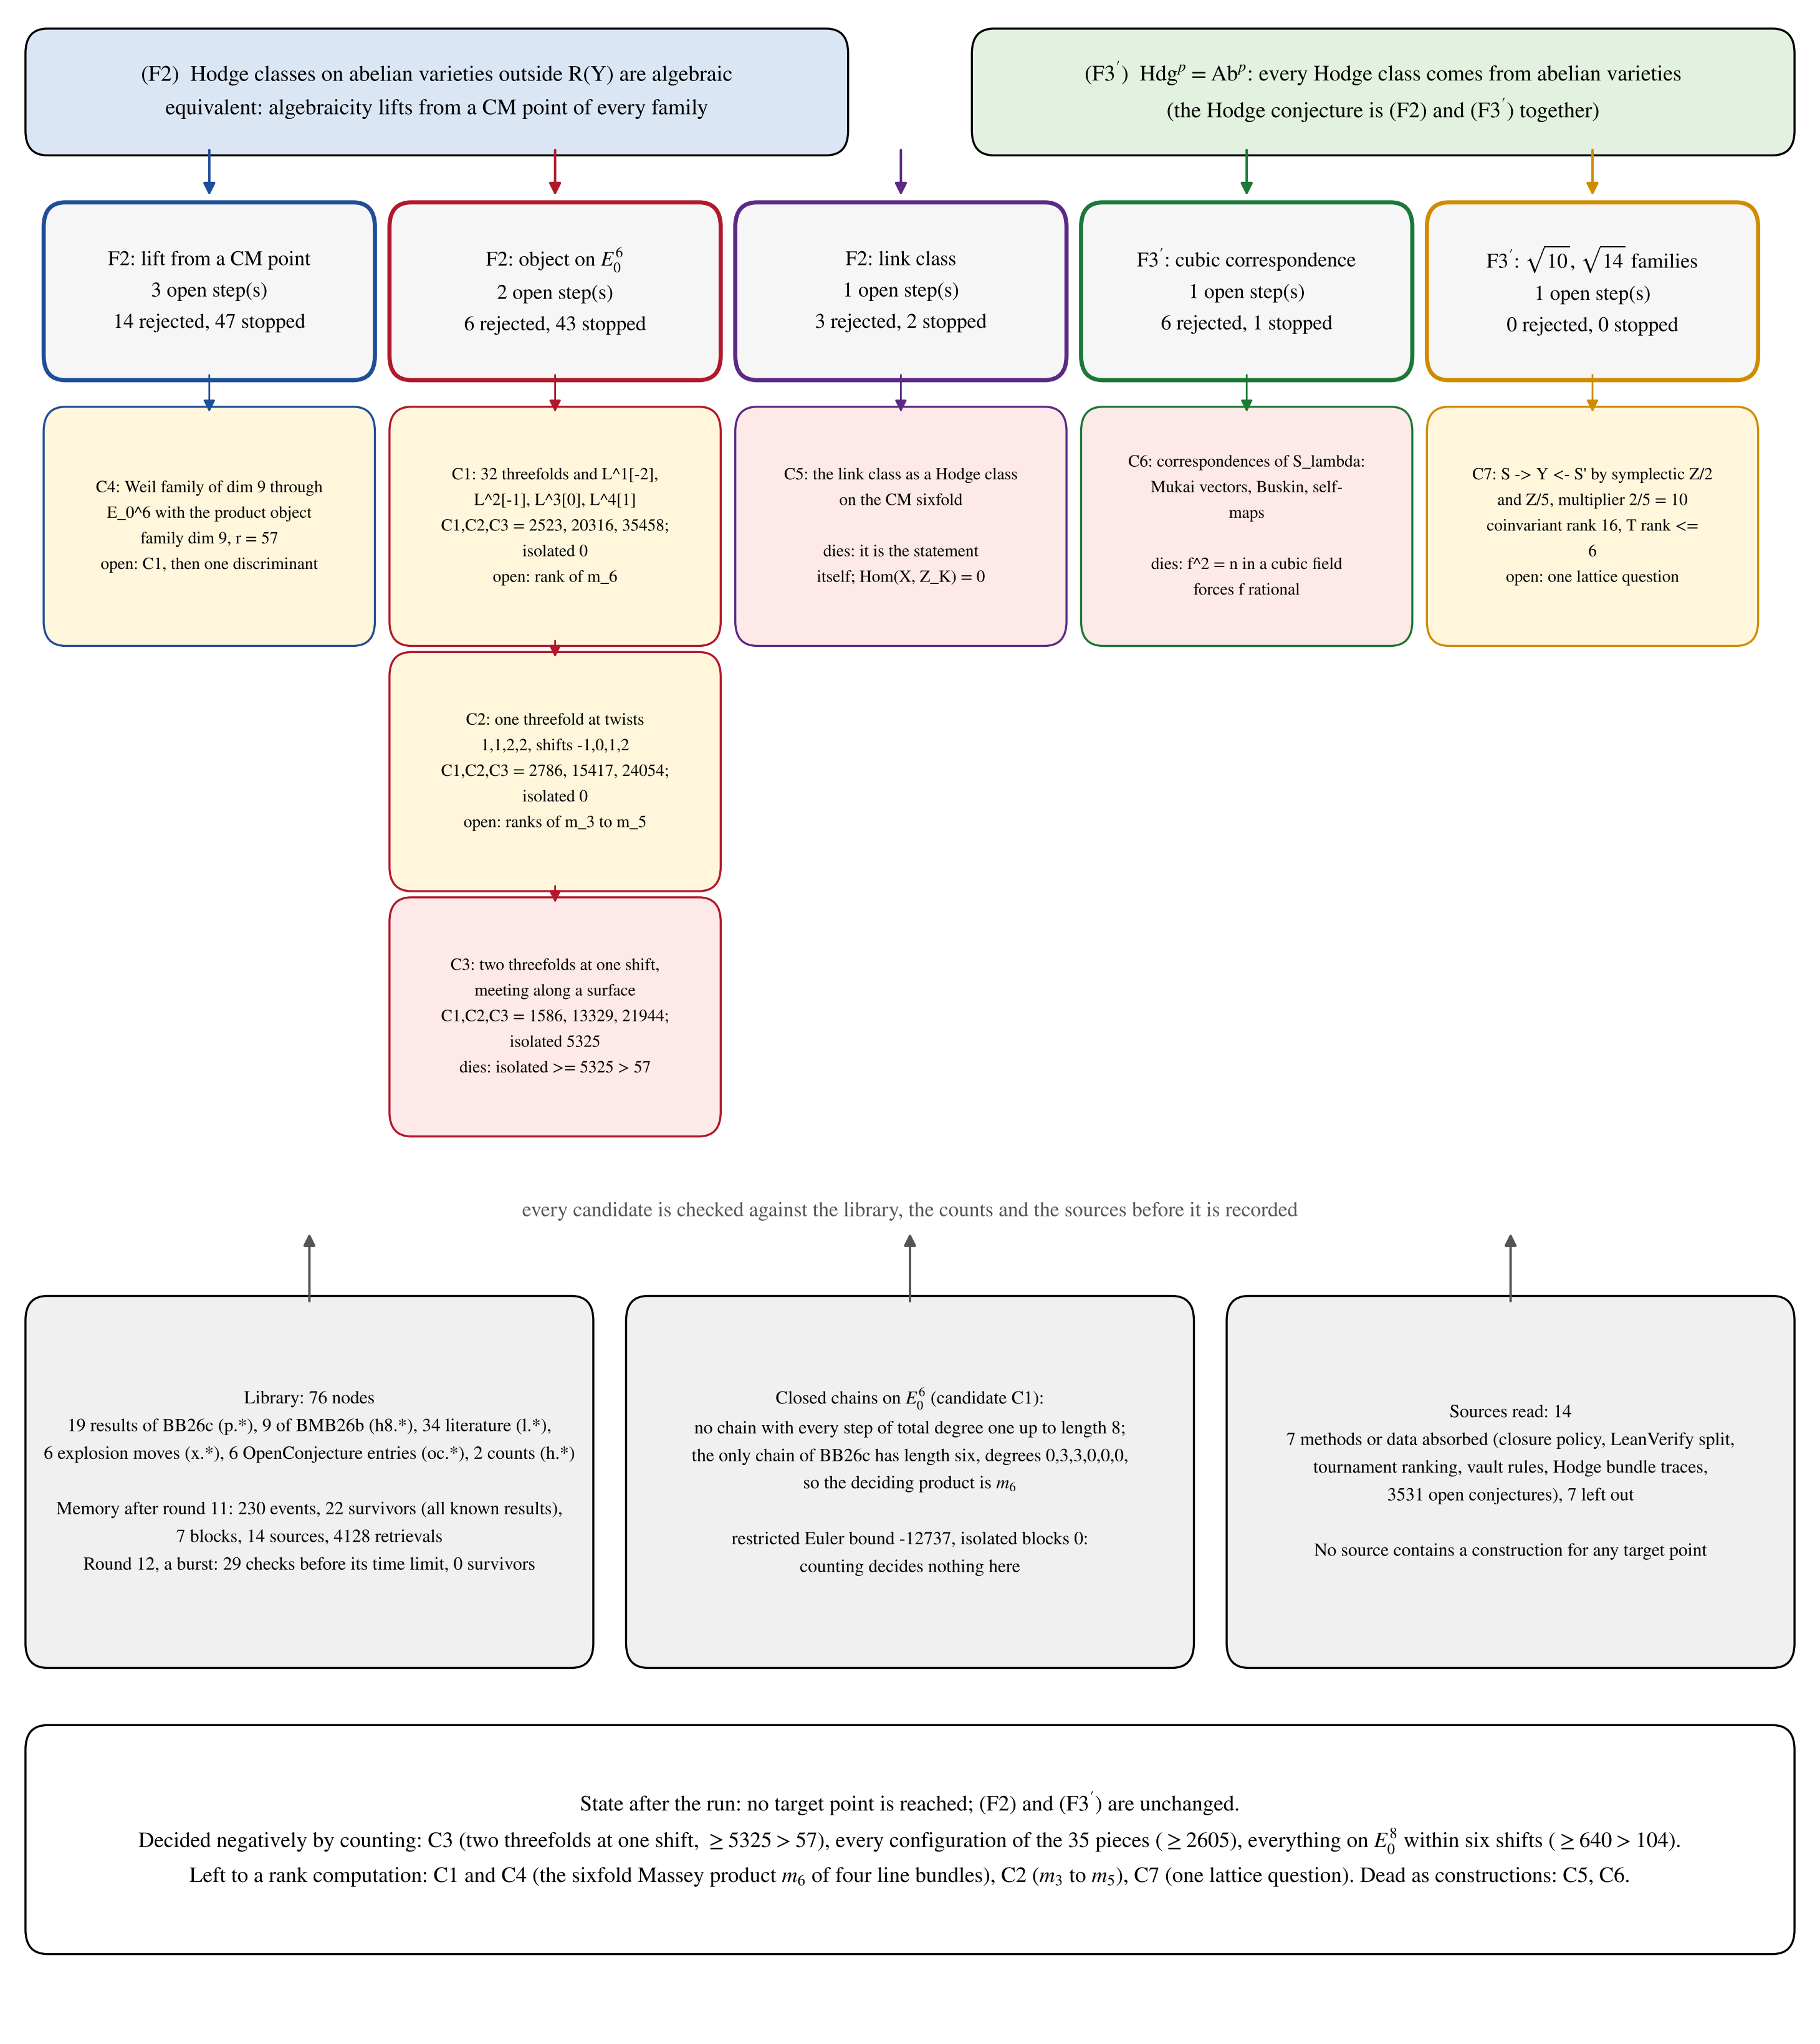
\includegraphics[width=0.98\textwidth,height=0.78\textheight,keepaspectratio]{figures/fig_hodgemap}
\Description{Map of the Hodge round: the two open statements at the top, the five target points with their gaps, and the eight candidates with their status.}
\caption{The map of the Hodge round. The two statements (F2) and (F3$'$) at the top, the five target points with their gap and their counts under them, the eight candidates under their targets (yellow open, red dead), and below them the three things every candidate is checked against before it is recorded: the library and the memory, the counting and chain results on $E_{0}^{6}$, and the fourteen sources. The bottom line is the state after the run.}
\label{fig:hodgemap}
\end{figure*}

\subsection{Sources}\label{ssec:hodgesources}

Fourteen sources were read during the round, and each is recorded in the memory with what was taken and what was left: a vault memory with embeddings and a knowledge graph, from which the community structure of the construction graph is kept and the server is not; a security reasoning stack with nothing for Hodge; an orchestration policy whose rule we adopt, that a problem is closed only after a kernel-checked Lean endpoint with an audited statement and the three standard axioms, never \texttt{native\_decide}, with evidence graded as lead, candidate, reproduced, formally verified and accepted; a Lean coding agent whose split of a theorem store from an axiom store the engine's Lean check follows; a hypothesis tournament whose Elo ranking orders the survivors of a burst; the output of a research agent on equivariant traces of the Hodge bundle over the moduli of curves, which enters as one construction; vault hygiene rules; four repositories with no mathematics; and the OpenConjecture collection of $3531$ open conjectures from the arXiv, in which a search finds $55$ on Hodge classes, abelian varieties, K3 surfaces and motives, six of which enter the library as conditional nodes. The memory shows that no source contains a construction for any target point; the ones that help change how the network keeps and ranks what it finds, not what it can find.

\subsection{What this round shows}\label{ssec:hodgeverdict}

Nothing closes. (F2) and (F3$'$) are where \cite{BB26c} left them, the gap of every target point is unchanged after the burst, and every decision is negative: the configuration (d) and every configuration of the $35$ pieces on $E_{0}^{6}$ are excluded by counting, every convolution of family (a) with at most seven line bundles by the parity of its chains against its Chern character, C7 by a rank count, two further candidates by arguments of \cite{BB26c} applied to them, and the sources add method and no construction. The decision on family (a) is the one the search did not reach: it comes from an argument by hand on the chains and the Chern character, not from a combination of library moves, and it replaces the sixfold Massey product of \cite{BB26c} by a parity count. What is left on $E_{0}^{6}$ is narrow and explicit: eight or more line bundles (C8), with $31$ arrangements of shifts at eight, and one threefold at several twists (C2), whose products $m_{3}$ to $m_{5}$ are a finite computation in the theta-function model of \cite{BMB26b}. The companion paper \cite{BMB26b} has carried out such computations for the fourfold products at distance two or more and for $E_{0}^{8}$ within six shifts, with the answer that they fail.

\section{What is proved and what is open}\label{sec:status}

\subsection{Proved}

Inside the model of Section~\ref{sec:model}, the paper determines the least cost of soundness. For finitely many candidates and exponential checks it is the entropy law, exact up to an additive term that is sharp (Theorem~\ref{thm:A}) and exact without remainder when the soundness is the reciprocal of an integer and the budget a power of it, where the optimal schedule is a Huffman code (Theorem~\ref{thm:C}). For checks of polynomial order the least cost is given in closed form by a R\'enyi entropy (Theorem~\ref{thm:D}), and for every cost function an infinite sequence of candidates admits a sound schedule of finite cost exactly when one series built from the concave conjugate of the cost converges (Theorem~\ref{thm:dual}). The same price, rescaled by the error rate of the generator, governs chains of improvements (Theorem~\ref{thm:B}), and checking only the outcome of a chain of $n$ steps is exponentially more expensive than checking every step (Theorem~\ref{thm:gating}). An infinite chain reaches a singularity soundly exactly when the costs of its checks have finite entropy in addition to a finite sum, which fails for a nonempty range of cost laws (Theorem~\ref{thm:E}, Corollary~\ref{cor:gap}); a branching takeoff with a fixed false acceptance rate keeps infinitely many errors on survival, and a sound one needs a number of runs that grows linearly with the generation (Theorem~\ref{thm:F}). In the Osgood model of growth every singular takeoff can be made sound with exponential checks, at a price of order $1/(\alpha-1)^{2}$ near the critical exponent, while polynomial checks move the threshold of a sound takeoff from $\alpha=1$ to $\alpha=1+s$ (Proposition~\ref{prop:osgood}).

None of this needs foresight or a single agent. A rule that sees only the past costs is sound for every future and pays over the offline optimum an excess of order $\frac{A}{L}\log\log\frac{A}{a_{1}}$, which no online rule avoids (Theorem~\ref{thm:G}), so sound singularities are reached online whenever they are reached at all (Corollary~\ref{cor:onlinesing}). Splitting the work among subagents is free when the budget is split in proportion to cost, and costs exactly a Kullback--Leibler divergence otherwise (Theorem~\ref{thm:H}); cheap checks before one exact check reduce the cost of the exact check to the correct candidates, up to a logarithmic premium (Theorem~\ref{thm:cascade}). Depth has a price of the same kind: $n$ verified layers that share one budget cost at least $n\log(n/\theta)$ nats of soundness, each added layer at least $\log((n+1)/\theta)$ more, and past a finite depth every tower costs more than any fixed amount (Theorem~\ref{thm:tower}).

Outside the model, three results come from the experiments. Theorem~\ref{thm:onethird} proves a lattice mass gap $m\ge-\log(3\beta_{W})$ for four-dimensional $\mathrm{SU}(2)$ on $\beta_{W}<\frac13$ by a gauge fixing with one fixed link per plaquette, and Proposition~\ref{prop:forestceiling} shows that no forest gauge fixing goes further; the theorem is proved here and has not been refereed. Lemma~\ref{lem:levelposet} reduces monochromatic sublattices of a level colouring to weighted posets, and with it Theorem~\ref{thm:fvalues} determines $f(n)$ for $n\le20$. Theorem~\ref{thm:seedbound} proves the seed conjecture for the reflexive polytopes of dimension four with a uniform bound: every descent to a minimal seed has at most $\seedBound$ steps, because each step lowers the lattice points of the polytope and raises those of its dual, and the pairs of the two counts that occur in the Kreuzer--Skarke list admit no longer chain.

The measurements of Section~\ref{sec:experiments} are these: typing the constructions is what lets the network reach a step that random pairing does not; Hebbian boosters do not improve on the unboosted network; memory halves the checks needed to reach the plateau and does not raise it; agents reach the plateau sooner and no further; and no transfer of a pattern in the matrix of Section~\ref{ssec:matrix} closes a blocking step. Construction mode rebuilds from the rules of Steinberg's problem the two gadgets of the counterexample of \cite{CHK17} and the counterexample itself, where random combination of library pieces finds nothing, and finds nothing on Erd\H{o}s's question for cycles of length $4$ to $6$ (Section~\ref{ssec:steinberg}). On three targets at equal budgets of exact checks, depth paid once: a second layer whose curriculum turns an easier gadget into a lemma reaches a gadget that the builder alone does not, a third layer adds nothing, and sharing one library and one set of weights shortens the step after the lemma (Section~\ref{ssec:towerbench}). Pointed at the Hodge conjecture alone, the network leaves the gap of every target point where it was after twelve rounds, including a burst that multiplied the cost of a round; counting excludes two of the configurations on $E_{0}^{6}$ left open in \cite{BB26c} and reduces two others to explicit Massey products (Section~\ref{sec:hodgeround}).

The finite inequalities behind these statements are proved in Lean~4 (Appendix~\ref{app:checks}). The probabilistic limit theorems, Wald's identity, the Kesten--Stigum theorem, L\'evy's conditional Borel--Cantelli lemma and the extinction theorem of Galton--Watson processes, are classical and are proved or cited in Appendix~\ref{app:derivations}; the asymptotics of $\zeta$ near $1$ are proved in the text.

\subsection{Open}

Six questions are left open, and each is a precise mathematical question.

\emph{Adaptive protocols.} Remark~\ref{rem:adaptive} shows that a protocol which looks at the outcomes of the checks can avoid the entropy term by halting at the first rejection, at the price of losing the correct work after it. Let a protocol be \emph{conservative} if, in every world, it keeps every correct candidate with probability one. Is the least worst-case expected cost of a conservative $\theta$-sound protocol equal to $\Vs(\theta)$ up to an additive $O(A)$? An adaptive protocol may let the number of runs of later checks depend on the results of earlier ones; since a correct candidate never fails, a conservative protocol learns nothing from the runs of a candidate that passes, and the question is whether the information it gains from rejections can be converted into a saving that is not $O(A)$.

\emph{Two-sided checks.} For checks that make errors on both sides Proposition~\ref{prop:twosided} gives the entropy law with the rate $D=\mathrm{KL}(\mathrm{Ber}(\frac12)\,\|\,\mathrm{Ber}(q))$ in the upper bound and $\log(1/q)$ in the lower bound. The exact rate of a sequential test with two error probabilities is Wald's \cite{Wal45}, and the question is whether the optimal schedule for many two-sided checks attains the entropy law with the Chernoff rate of the pair of hypotheses, in both directions.

\emph{Correlated runs.} The model assumes that the runs of a check are independent. A real verifier, a learned reward model or a test suite run on the same machine, has correlated errors, and repeated runs of a deterministic check gain nothing. The entropy law holds for every family of checks whose false acceptance probability after $r$ runs is at most $\eps^{r}$, whatever the mechanism; the open question is which checks used in practice have this property, with which $\eps$, and what replaces the law for those that do not.

\emph{Monochromatic sublattices.} Is $f(n)=O(n)$? For every $n\le20$ some level colouring is optimal (Theorem~\ref{thm:fvalues}); if level colourings are optimal for every $n$, Lemma~\ref{lem:levelposet} reduces the question to words in two letters.

\emph{The sharp seed constant.} What is the least $D$ such that every reflexive $4$-polytope reaches a seed in at most $D$ descent steps? It lies between $\seedLow$ and $\seedBound$ (Section~\ref{sec:seed}); in dimensions two and three it is $\seedTwo$ and $\seedThree$.

\emph{The online constant.} The upper and lower bounds of Theorem~\ref{thm:G} differ by a factor of four in the term $\frac{A_{N}}{L}\log\log\frac{A_{N}}{a_{1}}$. The exact constant is the least $\kappa$ such that a $\theta$-sound online rule has excess $(\kappa+o(1))\frac{A_{N}}{L}\log\log\frac{A_{N}}{a_{1}}$ on every sequence; the bounds give $\frac12\le\kappa\le2$.

\subsection{What is not claimed}

The paper does not claim that any existing system is sound or that an intelligence explosion will or will not occur. It does not claim progress on the five problems of Section~\ref{sec:benchmark} beyond the two results above: none of their pass lines is crossed, the Yang--Mills step lies below the crossover where the open problem begins, and the values of $f(n)$ do not decide whether $f(n)=O(n)$. The Steinberg gadgets are a rediscovery of a published construction, and the exclusions on $E_{0}^{6}$ leave (F2) and (F3$'$) open. The sixth line is crossed by the seed conjecture in the form of Section~\ref{sec:seed}; the sharp constant in dimension four is not determined, and the selection principle for string vacua from the same papers is not proved. Passing all six lines is a definition we use to score a proposer, not a property any system has shown. The theorems are statements about a model with independent runs, perfect completeness and schedules fixed in advance, and their value for a real system depends on how well it satisfies them. What is claimed is that inside the model the cost of soundness is computable, that it is an entropy, and that it divides the singular processes into those that can be made sound and those that cannot; and that on five open problems a typed crossing network with memory reaches what its libraries can reach at half the cost, and stops where the libraries stop, while construction mode writes down objects that no combination of the library reaches and has so far written down only known gadgets; and that on one open conjecture of mathematical physics the engine reached a proof with a uniform bound.


\appendix
\section{Classical facts used in the proofs}\label{app:derivations}

This appendix proves, or states with a precise reference, the classical results that the main text uses. Nothing here is new; the proofs are given so that the paper can be read without the references.

\subsection{Kraft's inequality and McMillan's theorem}\label{app:kraft}

Fix an integer $D\ge2$. A word of length $\ell$ over the alphabet $\{0,\dots,D-1\}$ is identified with the interval
\[
J(w)=\Bigl[\,\sum_{j=1}^{\ell}w_{j}D^{-j},\ \sum_{j=1}^{\ell}w_{j}D^{-j}+D^{-\ell}\Bigr)\subset[0,1),
\]
the set of reals in $[0,1)$ whose $D$-ary expansion, taken without a tail of digits $D-1$, begins with $w$. Two intervals $J(w)$ and $J(w')$ meet if and only if one of the words is a prefix of the other: if $w$ is a prefix of $w'$ then $J(w')\subset J(w)$, and otherwise the two expansions differ at some position not beyond the shorter length, so no real begins with both.

\begin{proposition}[Kraft]
Lengths $\ell_{1},\dots,\ell_{n}\in\NN$ are those of a $D$-ary prefix code if and only if $\sum_{i}D^{-\ell_{i}}\le1$.
\end{proposition}

\begin{proof}
If the words form a prefix code, the intervals $J(w_{i})$ are disjoint subsets of $[0,1)$ of lengths $D^{-\ell_{i}}$, so their lengths add up to at most $1$. Conversely, order the lengths so that $\ell_{1}\le\dots\le\ell_{n}$ and put $c_{i}=\sum_{j<i}D^{-\ell_{j}}$. Each $D^{-\ell_{j}}$ with $j<i$ is a multiple of $D^{-\ell_{i}}$, so $c_{i}D^{\ell_{i}}$ is an integer, and $c_{i}+D^{-\ell_{i}}\le\sum_{j}D^{-\ell_{j}}\le1$, so $0\le c_{i}D^{\ell_{i}}\le D^{\ell_{i}}-1$. Let $w_{i}$ be the expansion of this integer in base $D$ with exactly $\ell_{i}$ digits. Then $J(w_{i})=[c_{i},c_{i+1})$, these intervals are disjoint, and the words form a prefix code.
\end{proof}

\begin{proposition}[McMillan]
If a code with lengths $\ell_{1},\dots,\ell_{n}$ is uniquely decodable, that is, distinct finite sequences of codewords have distinct concatenations, then $\sum_{i}D^{-\ell_{i}}\le1$.
\end{proposition}

\begin{proof}
Let $M=\max_{i}\ell_{i}$ and $k\ge1$. Expanding the $k$-th power,
\[
\Bigl(\sum_{i}D^{-\ell_{i}}\Bigr)^{k}=\sum_{i_{1},\dots,i_{k}}D^{-(\ell_{i_{1}}+\dots+\ell_{i_{k}})}=\sum_{m=k}^{kM}N_{m}D^{-m},
\]
where $N_{m}$ is the number of $k$-tuples of codewords whose concatenation has length $m$. By unique decodability these concatenations are distinct words of length $m$, so $N_{m}\le D^{m}$ and the sum is at most $kM$. Hence $\sum_{i}D^{-\ell_{i}}\le(kM)^{1/k}$ for every $k$, and $(kM)^{1/k}\to1$.
\end{proof}

\subsection{Huffman's algorithm}\label{app:huffman}

Let $p_{1}\ge\dots\ge p_{n}\ge0$ with $\sum p_{i}=1$, and let $L_{D}(p)$ be the least value of $\sum_{i}p_{i}\ell_{i}$ over $\ell\in\NN^{n}$ with $\sum_{i}D^{-\ell_{i}}\le1$. The minimum exists: let $c_{0}$ be the cost of the code in which every word has length $\lceil\log_{D}n\rceil$; a vector of cost at most $c_{0}$ has $\ell_{i}\le c_{0}/p_{i}$ for every $i$ with $p_{i}>0$, and the cost does not depend on the other lengths, so it takes only finitely many values at most $c_{0}$. Huffman's algorithm \cite{Huf52} is the following recursion. If $n=1$ the code is the empty word. Otherwise add zero weights until $n\equiv1\pmod{D-1}$, merge the $D$ smallest weights into one symbol whose weight is their sum, solve the smaller problem, and give the $D$ merged symbols the codeword of their merger followed by each of the $D$ letters.

\begin{proposition}[Huffman]
The algorithm returns a prefix code of expected length $L_{D}(p)$.
\end{proposition}

\begin{proof}
\emph{Step 1: padding is free.} Adding a symbol of weight $0$ cannot lower the optimum, since removing a codeword from a code keeps Kraft's inequality and the cost. It does not raise it either, by the following argument. Let $\ell$ be optimal for $p$ with $n\not\equiv1\pmod{D-1}$, and let $M=\max\ell_{i}$. Since $D^{M-\ell_{i}}\equiv1\pmod{D-1}$, the integer $\sum_{i}D^{M-\ell_{i}}$ is congruent to $n$, and $D^{M}$ to $1$, modulo $D-1$; so $\sum_{i}D^{-\ell_{i}}<1$, the difference being a positive multiple of $D^{-M}$. Zero weights at lengths $M+1,\dots,M+k$ add $\sum_{j=1}^{k}D^{-M-j}<D^{-M}$ to the Kraft sum and nothing to the cost. So we may assume $n\equiv1\pmod{D-1}$.

\emph{Step 2: an optimal code with equality.} Among the optimal $\ell$ choose one with $\sum_{i}\ell_{i}$ least, and let $M=\max\ell_{i}$; if $M=0$ then $n=1$. By the congruence of Step~1, now with $n\equiv1$, the deficit $\Delta=1-\sum_{i}D^{-\ell_{i}}$ satisfies $\Delta D^{M}\equiv0\pmod{D-1}$. If $\Delta>0$, then $\Delta\ge(D-1)D^{-M}$, and shortening one word of length $M$ by one letter adds $(D-1)D^{-M}$ to the Kraft sum, keeps it at most $1$, does not raise the cost and lowers $\sum\ell_{i}$, a contradiction. So $\sum_{i}D^{-\ell_{i}}=1$.

\emph{Step 3: the smallest weights are deepest.} If $p_{i}>p_{j}$ and $\ell_{i}>\ell_{j}$, exchanging the two lengths lowers the cost by $(p_{i}-p_{j})(\ell_{i}-\ell_{j})>0$; so in an optimal code $p_{i}>p_{j}$ implies $\ell_{i}\le\ell_{j}$, and among equal weights the lengths may be permuted freely. Multiplying the equality of Step~2 by $D^{M}$, every word shorter than $M$ contributes a multiple of $D$, so the number of words of length $M$ is a positive multiple of $D$, hence at least $D$. By the exchange we may assume that the $D$ smallest weights $p_{n-D+1},\dots,p_{n}$ have length $M$.

\emph{Step 4: the recursion.} Let $p'$ be the vector of $n-D+1\equiv1\pmod{D-1}$ weights obtained by merging the $D$ smallest into $\sigma=p_{n-D+1}+\dots+p_{n}$. The lengths of Step~3, with the merged symbol at length $M-1$, satisfy Kraft's inequality for $p'$, since $D\cdot D^{-M}=D^{-(M-1)}$, and have cost $\sum_{i}p_{i}\ell_{i}-\sigma$; so $L_{D}(p')\le L_{D}(p)-\sigma$. Conversely, a code for $p'$ in which the merged symbol has length $\ell'$ gives a code for $p$ by giving the $D$ merged symbols length $\ell'+1$, with the same Kraft sum and cost increased by $\sigma$; so $L_{D}(p)\le L_{D}(p')+\sigma$. Hence $L_{D}(p)=L_{D}(p')+\sigma$, which is the recursion of the algorithm, and induction on $n$ concludes.
\end{proof}

\subsection{Wald's identity and the geometric number of retries}\label{app:wald}

Let $c_{1},c_{2},\dots$ be independent and identically distributed costs of successive candidates, with finite mean, and let $K$ be the index of the first candidate kept, where whether candidate $j$ is kept depends only on candidate $j$, with probability $s>0$. Then $K$ is geometric, $\EE K=1/s$, and $\EE\sum_{j\le K}c_{j}=\EE K\cdot\EE c_{1}$ \cite{Wal45}. Indeed $\{K\ge j\}$ is determined by the candidates $1,\dots,j-1$ and is therefore independent of $c_{j}$, so by monotone convergence $\EE\sum_{j\le K}c_{j}=\sum_{j}\EE[c_{j}]\PR(K\ge j)=\EE c_{1}\sum_{j}\PR(K\ge j)=\EE c_{1}\,\EE K$. This is the identity used in Lemma~\ref{lem:onestep}.

\subsection{Products and the Borel--Cantelli lemmas}\label{app:bc}

Let $0\le\pi_{n}<1$. If $\sum\pi_{n}<\infty$ then $\prod_{n}(1-\pi_{n})>0$: for $n$ large $\pi_{n}\le\frac12$, and $\log(1-x)\ge-2x$ on $[0,\frac12]$, so the logarithm of the tail of the product is at least $-2\sum_{n\ge N}\pi_{n}>-\infty$, and the first factors are positive. If $\sum\pi_{n}=\infty$ then $\prod_{n\ge N}(1-\pi_{n})\le\exp(-\sum_{n\ge N}\pi_{n})=0$ for every $N$. For independent events $E_{n}$ with $\PR(E_{n})=\pi_{n}$ the second statement is the second Borel--Cantelli lemma, since $\PR(\text{no }E_{n}\text{ with }n\ge N)=\prod_{n\ge N}(1-\pi_{n})=0$ for every $N$; the first Borel--Cantelli lemma, that $\sum\PR(E_{n})<\infty$ implies that only finitely many $E_{n}$ occur, needs no independence, because $\EE\sum\ind_{E_{n}}=\sum\PR(E_{n})<\infty$ \cite{Bor09,Dur19}.

\subsection{L\'evy's conditional Borel--Cantelli lemma}\label{app:levy}

Let $(\mathcal F_{k})$ be a filtration, $B_{k}\in\mathcal F_{k}$ and $p_{k}=\PR(B_{k}\mid\mathcal F_{k-1})$. Then, up to a null set, $\{B_{k}\text{ infinitely often}\}=\{\sum_{k}p_{k}=\infty\}$ \cite[Section~4.3]{Dur19}.

\begin{proof}
$M_{n}=\sum_{k\le n}(\ind_{B_{k}}-p_{k})$ is a martingale with increments bounded by $1$. For such a martingale, almost surely either $M_{n}$ converges to a finite limit or $\limsup M_{n}=+\infty$ and $\liminf M_{n}=-\infty$ \cite[Section~4.3]{Dur19}. Write $\sum_{k\le n}\ind_{B_{k}}=M_{n}+\sum_{k\le n}p_{k}$; the left side is nonnegative and nondecreasing. On $\{\sum p_{k}<\infty\}$, $\liminf M_{n}=-\infty$ would make the left side negative, so $M_{n}$ converges and $\sum\ind_{B_{k}}<\infty$. On $\{\sum p_{k}=\infty\}$, if $\sum\ind_{B_{k}}<\infty$ then $M_{n}\to-\infty$, which is neither alternative; so $\sum\ind_{B_{k}}=\infty$.
\end{proof}

\subsection{Cauchy's condensation test}\label{app:condensation}

If $b_{n}\ge0$ is nonincreasing for $n\ge n_{0}$, then $\sum_{n}b_{n}<\infty$ if and only if $\sum_{k}2^{k}b_{2^{k}}<\infty$. Indeed, for $2^{k}\ge n_{0}$ the block $2^{k}\le n<2^{k+1}$ has $2^{k}$ terms, each between $b_{2^{k+1}}$ and $b_{2^{k}}$, so its sum lies between $\frac12\,2^{k+1}b_{2^{k+1}}$ and $2^{k}b_{2^{k}}$. For $b_{n}=1/(n\log^{c}n)$, which is eventually nonincreasing for every real $c$, the condensed terms are $(k\log2)^{-c}$, and their series converges if and only if $c>1$.

\subsection{Sums and integrals of unimodal functions}\label{app:zeta}

Let $f\ge0$ be integrable on $[1,\infty)$, nondecreasing on $[1,x_{0}]$ and nonincreasing on $[x_{0},\infty)$, with maximum $M_{f}=f(x_{0})$. Then
\[
\Bigl|\sum_{n\ge1}f(n)-\int_{1}^{\infty}f(x)\,dx\Bigr|\le M_{f}.
\]
Let $N=\lfloor x_{0}\rfloor$. For $1\le n\le N-1$, $f$ is nondecreasing on $[n,n+1]$, so $f(n)\le\int_{n}^{n+1}f\le f(n+1)$; for $n\ge N+1$, $f$ is nonincreasing on $[n,n+1]$, so $f(n+1)\le\int_{n}^{n+1}f\le f(n)$. Summing,
\[
\begin{aligned}
\sum_{n\ge1}f(n)&\le\int_{1}^{N}f+f(N)+f(N+1)+\int_{N+1}^{\infty}f,\\
\sum_{n\ge1}f(n)&\ge f(1)+\int_{1}^{N}f+\int_{N+1}^{\infty}f .
\end{aligned}
\]
On $[N,N+1]$ the function is at least $\min(f(N),f(N+1))$, because it rises and then falls there; so $\int_{N}^{N+1}f\ge\min(f(N),f(N+1))$, and the first inequality gives $\sum f(n)\le\int_{1}^{\infty}f+\max(f(N),f(N+1))$. The second gives $\sum f(n)\ge\int_{1}^{\infty}f-\int_{N}^{N+1}f\ge\int_{1}^{\infty}f-M_{f}$. For $f(x)=x^{-p}\log x$ with $p>1$ one has $x_{0}=e^{1/p}$, $M_{f}=1/(pe)$ and $\int_{1}^{\infty}f=1/(p-1)^{2}$, which is the estimate used in Proposition~\ref{prop:powerlaw}; the same argument, with $x_{0}=1$, gives $1/(p-1)\le\zeta(p)\le1+1/(p-1)$.

\subsection{Extinction of a Galton--Watson process}\label{app:gw}

Let $N\ge0$ be an integer random variable with $f(z)=\EE z^{N}$, mean $m=f'(1^{-})\in[0,\infty]$ and $\PR(N=1)<1$, and let $(Z_{k})$ be the Galton--Watson process with $Z_{0}=1$ and offspring law $N$. Then the extinction probability $e=\PR(Z_{k}=0\text{ for some }k)$ is the least root of $f(z)=z$ in $[0,1]$, and $e=1$ if and only if $m\le1$ \cite{AN72,WG75}.

\begin{proof}
Conditioning on the first generation, the generating function of $Z_{k}$ is the $k$-fold composition $f_{k}=f\circ\dots\circ f$, so $\PR(Z_{k}=0)=f_{k}(0)$. These numbers increase with $k$ to $e$, and $f(e)=e$ by continuity of $f$ on $[0,1]$. If $z^{\ast}\in[0,1]$ is a root, then $f_{k}(0)\le f_{k}(z^{\ast})=z^{\ast}$ because $f$ is nondecreasing, so $e\le z^{\ast}$: $e$ is the least root. If $\PR(N\ge2)=0$, then $f(z)=\PR(N=0)+\PR(N=1)z$ with $m=\PR(N=1)<1$, and $f(z)>z$ on $[0,1)$, so $e=1$. Otherwise $f'$ is strictly increasing on $[0,1)$. If $m\le1$, then $f'(z)<1$ on $[0,1)$, so $f(z)-z$ is strictly decreasing there with limit $0$ at $1$, hence positive, and the only root is $1$. If $m>1$, then $f(z)<z$ for $z<1$ close to $1$, while $f(0)\ge0$, so there is a root in $[0,1)$, and $e<1$.
\end{proof}

The theorem of Kesten and Stigum \cite{KS66}, used in the proof of Theorem~\ref{thm:F}, is not proved here: if $1<m<\infty$, the martingale $Z_{k}/m^{k}$ converges almost surely to a limit $W$, and $W>0$ almost surely on survival if and only if $\EE N\log N<\infty$; the proof is in \cite[Chapter~I]{AN72}.

\section{Formal proofs and numerical checks}\label{app:checks}

\subsection{The Lean development}

The finite inequalities of the paper are proved in Lean~4 with Mathlib, in fifteen files and sixty-five theorems, listed in Tables~\ref{tab:lean} and~\ref{tab:lean2}. Every theorem depends only on the three standard axioms of Lean, propositional extensionality, the axiom of choice and the soundness of quotients; the command \texttt{\#print axioms} is run on each of them, and no theorem uses \texttt{sorry}. The statements are over the real numbers, with finite sums indexed by a \texttt{Finset} and infinite ones expressed by \texttt{Summable}; in them $\sigma$ is the polynomial order written $s$ in the text, and $(1/D)^{r}$ is $\eps^{r}$ with $\eps=1/D$.

The formal statements cover the deterministic content of the main theorems: Gibbs' inequality in the form used for the entropy law, the lower bound and the two properties of the ceiling schedule (Theorem~\ref{thm:A}), the correspondence between schedules and Kraft vectors and the shifted cost (Theorem~\ref{thm:C}), H\"older's lower bound and the optimal allocation of the R\'enyi law (Theorem~\ref{thm:D}) with the summability criterion for polynomial checks, both halves of the duality criterion (Theorem~\ref{thm:dual}), the inequalities for clean runs and random schedules (Propositions~\ref{prop:clean} and~\ref{prop:random}), the precision and cost identities of the gating theorem (Theorem~\ref{thm:gating}), the summability criterion for sound singular chains with both directions (Theorem~\ref{thm:E}(iii)), the two Borel--Cantelli statements for false acceptances (Theorem~\ref{thm:E}(i)), the divergence and amplification statements of the branching theorem (Theorem~\ref{thm:F}), the online, subagent, cascade and gap laws (Theorems~\ref{thm:G}, \ref{thm:H}, \ref{thm:cascade} and~\ref{thm:I}), and the four parts of the tower law (Theorem~\ref{thm:tower}). The limit theorems of probability (Wald's identity, the extinction theorem, the Kesten--Stigum theorem and L\'evy's lemma), the asymptotics of $\zeta$ and of the entropies in Propositions~\ref{prop:powerlaw} and~\ref{prop:osgood}, and the estimates of Proposition~\ref{prop:twosided} are proved in the text and are not formalised.

\begin{table*}[t]
\caption{The sixty-five theorems of the Lean development, by file. The third column gives the statement in the notation of the paper and the fourth the result in which it is used. Sums over $i$ are finite; sums over $n$ or $k$ are infinite and ``$\sum<\infty$'' means summability.}
\label{tab:lean}
\centering
\footnotesize
\begin{tabular}{@{}l l p{0.53\textwidth} l@{}}
\toprule
File & Theorem & Statement & Used in \\
\midrule
\texttt{Basic} & \lean{gibbs\_term} & $x\log\frac1x\le x\log\frac1y+y-x$ for $x,y>0$ & Lemma~\ref{lem:gibbs} \\
 & \lean{entropy\_term} & $a\log\frac Aa+a\log\frac1\theta\le a\log\frac1b+\frac{Ab}\theta-a$ & Lemma~\ref{lem:entropyterm} \\
 & \lean{log\_inv\_pow} & $\log(1/\eps^{r})=r\log(1/\eps)$ & Theorem~\ref{thm:A} \\
 & \lean{log\_inv\_pos} & $\log(1/\eps)>0$ for $0<\eps<1$ & Theorem~\ref{thm:A} \\
\texttt{EntropyLaw} & \lean{entropy\_lower} & $\sum\beta_{i}\le\theta\Rightarrow\sum a_{i}\log\frac A{a_{i}}+A\log\frac1\theta\le\sum a_{i}\log\frac1{\beta_{i}}$ & Proposition~\ref{prop:entropyineq} \\
 & \lean{verification\_lower} & $\sum\eps^{r_{i}}\le\theta\Rightarrow\frac AL(H+\log\frac1\theta)\le\sum a_{i}r_{i}$ & Theorem~\ref{thm:A} \\
 & \lean{ceilSchedule\_sound} & the ceiling schedule has $\sum\eps^{r_{i}}\le\theta$ & Theorem~\ref{thm:A} \\
 & \lean{ceilSchedule\_cost} & the ceiling schedule costs at most $\frac AL(H+\log\frac1\theta)+A$ for $\theta\le1$ & Theorem~\ref{thm:A} \\
\texttt{Kraft} & \lean{kraft\_of\_schedule} & $\sum D^{-r_{i}}\le D^{-k}\Rightarrow r_{i}\ge k$ and $\sum D^{-(r_{i}-k)}\le1$ & Lemma~\ref{lem:kraftsound}(i) \\
 & \lean{schedule\_of\_kraft} & $\sum D^{-\ell_{i}}\le1\Rightarrow\sum D^{-(\ell_{i}+k)}\le D^{-k}$ & Lemma~\ref{lem:kraftsound}(ii) \\
 & \lean{shifted\_cost} & $\sum a_{i}(\ell_{i}+k)=kA+\sum a_{i}\ell_{i}$ & Lemma~\ref{lem:kraftsound}(iii) \\
\texttt{Renyi} & \lean{renyi\_lower} & $\sum\delta_{i}\le\theta\Rightarrow(\sum a_{i}^{1/(1+s)})^{1+s}\le\theta^{s}\sum a_{i}\delta_{i}^{-s}$ & Theorem~\ref{thm:D} \\
 & \lean{renyi\_attain} & $\delta_{i}=\theta a_{i}^{1/(1+s)}/S$ has $\sum\delta_{i}=\theta$ and cost $\theta^{-s}S^{1+s}$ & Theorem~\ref{thm:D} \\
 & \lean{poly\_schedule\_iff} & a positive $\delta$ with $\sum\delta_{n}<\infty$, $\sum a_{n}\delta_{n}^{-s}<\infty$ exists $\iff\sum a_{n}^{1/(1+s)}<\infty$ & Corollary~\ref{cor:dualcases}(ii) \\
\texttt{Duality} & \lean{dualCost\_nonneg} & $\psi(u)\ge0$ for $u\ge0$ & Theorem~\ref{thm:dual} \\
 & \lean{dualCost\_le} & $\psi(u)\le\kappa(\delta)+u\delta$ for $\delta\in(0,1]$ & Theorem~\ref{thm:dual} \\
 & \lean{dual\_summable\_of\_schedule} & a sound allocation of finite cost gives $\sum a_{n}\psi(\lambda/a_{n})<\infty$ for every $\lambda>0$ & Theorem~\ref{thm:dual} \\
 & \lean{schedule\_of\_dual\_summable} & $\sum a_{n}\psi(\lambda/a_{n})<\infty$ for one $\lambda>0$ gives a sound allocation of finite cost & Theorem~\ref{thm:dual} \\
\texttt{Clean} & \lean{clean\_le\_exp} & $\prod(1-q_{i})\le e^{-\sum q_{i}}$ for $q_{i}\le1$ & Proposition~\ref{prop:clean} \\
 & \lean{clean\_ge} & $1-\sum q_{i}\le\prod(1-q_{i})$ for $0\le q_{i}\le1$ & Proposition~\ref{prop:clean} \\
 & \lean{clean\_budget} & $\prod(1-q_{i})\ge1-\theta\Rightarrow\sum q_{i}\le\log\frac1{1-\theta}$ & Proposition~\ref{prop:clean} \\
\texttt{Adaptive} & \lean{jensen\_repetition} & $\eps^{\sum w_{j}r_{j}}\le\sum w_{j}\eps^{r_{j}}$ for weights $w$ & Proposition~\ref{prop:random} \\
 & \lean{randomised\_budget} & a random schedule within budget in mean has its mean within budget & Proposition~\ref{prop:random} \\
\texttt{Gating} & \lean{step\_precision} & $\frac{(1-\rho)(1-\eta)}{(1-\rho)(1-\eta)+\rho\delta}=\frac1{1+x}$ & Theorem~\ref{thm:gating}(i) \\
 & \lean{precision\_bounds} & $e^{-\sum x_{i}}\le\prod(1+x_{i})^{-1}\le e^{-\sum x_{i}/(1+x_{i})}$ & Theorem~\ref{thm:gating}(i) \\
 & \lean{outcome\_precision} & $\frac{c(1-\eta_{o})}{c(1-\eta_{o})+(1-c)\delta_{o}}=\bigl(1+\frac{(1-c)\delta_{o}}{c(1-\eta_{o})}\bigr)^{-1}$ & Theorem~\ref{thm:gating}(ii) \\
 & \lean{separation} & cost ratio $(1-\rho)^{-n}$ and $1+n\rho\le(1-\rho)^{-n}$ & Theorem~\ref{thm:gating}(iii) \\
\bottomrule
\end{tabular}
\end{table*}

\begin{table*}[t]
\caption{The Lean development, continued.}
\label{tab:lean2}
\centering
\footnotesize
\begin{tabular}{@{}l l p{0.53\textwidth} l@{}}
\toprule
File & Theorem & Statement & Used in \\
\midrule
\texttt{Singularity} & \lean{entropy\_summable\_of\_schedule} & $\sum\eps^{r_{n}}<\infty$, $\sum a_{n}r_{n}<\infty$, $a_{n}\le1\Rightarrow\sum a_{n}\log\frac1{a_{n}}<\infty$ & Theorem~\ref{thm:E}(iii) \\
 & \lean{costSchedule\_pow\_le} & $r_{n}=\lceil\log(1/a_{n})/L\rceil$ has $\eps^{r_{n}}\le a_{n}$ & Proposition~\ref{prop:integer} \\
 & \lean{schedule\_of\_entropy\_summable} & $\sum a_{n}<\infty$, $\sum a_{n}\log\frac1{a_{n}}<\infty$ make that schedule sound and of finite cost & Theorem~\ref{thm:E}(iii) \\
 & \lean{sound\_schedule\_iff} & for $\sum a_{n}<\infty$, $a_{n}\le1$: a sound schedule of finite cost exists $\iff\sum a_{n}\log\frac1{a_{n}}<\infty$ & Proposition~\ref{prop:integer} \\
 & \lean{shift\_schedule} & $\eps^{r_{n}+k}=\eps^{k}\eps^{r_{n}}$ & Theorem~\ref{thm:E}(iii) \\
\texttt{Soundness} & \lean{false\_accepts\_finite} & $\PR(E_{n})\le Cq_{n}$, $\sum q_{n}<\infty\Rightarrow\PR(E_{n}\text{ i.o.})=0$ & Theorem~\ref{thm:E}(i) \\
 & \lean{false\_accepts\_infinite} & independent $E_{n}$, $\PR(E_{n})\ge bq_{n}$, $b>0$, $\sum q_{n}=\infty\Rightarrow\PR(E_{n}\text{ i.o.})=1$ & Theorem~\ref{thm:E}(i) \\
 & \lean{any\_false\_accept\_le} & $\PR(\bigcup E_{n})\le C\sum q_{n}$ & Theorem~\ref{thm:E}(i) \\
\texttt{Branching} & \lean{contamination\_diverges} & $\sum m^{k}\delta=\infty$ for $m\ge1$, $\delta>0$ & Theorem~\ref{thm:F} \\
 & \lean{amplified\_term} & $k\log(2m)\le r_{k}L\Rightarrow m^{k}\eps^{r_{k}}\le2^{-k}$ & Theorem~\ref{thm:F} \\
 & \lean{amplified\_summable} & under the same hypothesis $\sum m^{k}\eps^{r_{k}}<\infty$ & Theorem~\ref{thm:F} \\
 & \lean{amplified\_schedule\_ok} & $r_{k}=\lceil k\log(2m)/L\rceil$ satisfies that hypothesis & Theorem~\ref{thm:F} \\
\texttt{Online} & \lean{ratio\_le\_log} & $1-s/t\le\log(t/s)$ for $s,t>0$ & Theorem~\ref{thm:G} \\
 & \lean{telescope\_step} & $\frac{y-x}{(1+y)^{2}}\le\frac1{1+x}-\frac1{1+y}$ for $0\le x\le y$ & Theorem~\ref{thm:G} \\
 & \lean{telescope\_sum} & $\sum_{n}\frac{u_{n+1}-u_{n}}{(1+u_{n+1})^{2}}\le\frac1{1+u_{0}}-\frac1{1+u_{N}}$ for monotone $u\ge0$ & Theorem~\ref{thm:G} \\
 & \lean{onlineWeight\_sum\_le} & $\sum_{n<N}w_{n}\le1$ for every sequence of positive costs & Theorem~\ref{thm:G} \\
 & \lean{onlineWeight\_pos} & $w_{n}>0$ & Theorem~\ref{thm:G} \\
 & \lean{onlineSchedule\_sound} & the online rule \eqref{eq:onlinerule} has $\sum_{n<N}\eps^{r_{n}}\le\theta$ for every $N$ & Theorem~\ref{thm:G} \\
 & \lean{small\_weight\_often} & $w\ge0$, $\sum_{n<N}w_{n}\le1$ for all $N\Rightarrow w_{N}\le\frac1{N+1}$ infinitely often & Theorem~\ref{thm:G} \\
 & \lean{online\_lower} & a $\theta$-sound schedule has $r_{N}L\ge\log\frac{N+1}\theta$ infinitely often & Theorem~\ref{thm:G} \\
 & \lean{doubling\_sum} & $\sum_{k<N}\frac{k+1}{2^{k+1}}=2-\frac{N+2}{2^{N}}$ & Theorem~\ref{thm:G} \\
\texttt{Agents} & \lean{groupCost\_pos} & $A_{k}>0$ for a nonempty group & Theorem~\ref{thm:H} \\
 & \lean{groupCost\_sum} & $\sum_{k}A_{k}=A$ & Theorem~\ref{thm:H} \\
 & \lean{chain\_rule} & $\sum a_{i}\log\frac A{a_{i}}=\sum_{k}A_{k}\log\frac A{A_{k}}+\sum_{k}\sum_{i\in G_{k}}a_{i}\log\frac{A_{k}}{a_{i}}$ & Theorem~\ref{thm:H}(i) \\
 & \lean{split\_lower} & $\sum\theta_{k}\le\theta\Rightarrow$ the group lower bounds add up to at least the flat one & Theorem~\ref{thm:H}(ii) \\
 & \lean{proportional\_split} & the ceiling schedule of $G_{k}$ at budget $\theta A_{k}/A$ is the flat one on $G_{k}$ & Theorem~\ref{thm:H}(iii) \\
 & \lean{cascade\_lower} & $br+c\rho\eps^{r}\ge\frac bL(1+\log\frac{c\rho L}b)$ for every $r$ & Theorem~\ref{thm:cascade} \\
 & \lean{cascade\_upper} & $b\le c\rho L\Rightarrow$ $r=\lceil\frac1L\log\frac{c\rho L}b\rceil$ costs at most that plus $b$ & Theorem~\ref{thm:cascade} \\
\texttt{Gap} & \lean{search\_lower} & $\sum q=1\Rightarrow(\sum a_{j})^{2}\le\sum a_{j}^{2}/q_{j}$, with $a_{j}=\sqrt{\pi_{j}}$ & Theorem~\ref{thm:I} \\
 & \lean{search\_optimal} & equality at $q_{j}=a_{j}/\sum a$ & Theorem~\ref{thm:I} \\
 & \lean{search\_chi2} & $\sum a_{j}^{2}/q_{j}=(\sum a)^{2}(1+\chi^{2}(r\|q))$ with $r_{j}=a_{j}/\sum a$ & Theorem~\ref{thm:I} \\
 & \lean{search\_mix} & $q\ge\lambda r\Rightarrow\sum a_{j}^{2}/q_{j}\le(\sum a)^{2}/\lambda$ & Theorem~\ref{thm:I} \\
\texttt{Tower} & \lean{tower\_cost\_lower} & $\beta_{k}>0$, $\sum_{k<n}\beta_{k}\le\theta\Rightarrow n\log\frac n\theta\le\sum_{k<n}\log\frac1{\beta_{k}}$ & Theorem~\ref{thm:tower}(i) \\
 & \lean{tower\_checks\_lower} & $\sum_{k<n}\eps^{r_{k}}\le\theta\Rightarrow n\log\frac n\theta/\log\frac1\eps\le\sum_{k<n}r_{k}$ & Theorem~\ref{thm:tower}(i) \\
 & \lean{tower\_increment} & $\log\frac{n+1}\theta\le(n+1)\log\frac{n+1}\theta-n\log\frac n\theta$ & Theorem~\ref{thm:tower}(ii) \\
 & \lean{tower\_increment\_unbounded} & $\log\frac{n+1}\theta\to\infty$ & Theorem~\ref{thm:tower}(ii) \\
 & \lean{tower\_saturates} & $S_{n}\ge B$, $V_{n}\ge c\,n\log\frac n\theta$, $c>0$, $\theta\le1\Rightarrow S_{n}+V_{n}>T_{1}$ for all large $n$ & Theorem~\ref{thm:tower}(iii) \\
 & \lean{stage\_cost\_diverges} & $\beta_{k}>0$, $\sum\beta_{k}<\infty\Rightarrow\log\frac1{\beta_{k}}\to\infty$ & Theorem~\ref{thm:tower}(iv) \\
\bottomrule
\end{tabular}
\end{table*}

\subsection{Numerical checks}

Independent programs test the closed forms of the paper against exhaustive searches, exact optima and simulation, on instances drawn with fixed seeds. They are listed in Table~\ref{tab:checks}; the shell script that runs them also builds the Lean development and prints the axioms of every theorem; the programs run $55{,}271$ checks in all, with no failure. The checks are not part of any proof. They guard against errors in the statements: a wrong constant, a reversed inequality or a misprinted formula would make one of them fail. The numerical values quoted in the text, in Tables~\ref{tab:huffman} and~\ref{tab:gw} and in the figures are produced by the same programs.

\begin{table}[!htb]
\caption{The numerical checks.}
\label{tab:checks}
\centering
\footnotesize
\begin{tabular}{@{}l p{0.56\columnwidth} r@{}}
\toprule
Language & What is checked & Checks \\
\midrule
Python & \rr Theorems~\ref{thm:A}, \ref{thm:C}: bounds and Huffman cost against exact optima & 649 \\
Python & \rr Theorem~\ref{thm:gating}: costs and precisions against simulation & 533 \\
Python & \rr Theorems~\ref{thm:D}, \ref{thm:dual}: R\'enyi optimum, dual costs & 20{,}850 \\
Python & \rr Theorem~\ref{thm:E}, Propositions~\ref{prop:powerlaw}, \ref{prop:osgood} & 241 \\
Python & \rr Theorem~\ref{thm:G}: online soundness, bounds, doubling lower bound & 1{,}581 \\
Python & \rr Theorems~\ref{thm:H}, \ref{thm:cascade}: chain rule, split price, cascades & 8{,}104 \\
Python & \rr Theorem~\ref{thm:F}: takeoff, kept errors, amplified checks & 2{,}432 \\
Python & \rr Theorem~\ref{thm:I}, Propositions~\ref{prop:learnrate}, \ref{prop:spiking}: gap law, square-root sampling, spiking selector & 12{,}081 \\
C & \rr Theorem~\ref{thm:C}: exhaustive search over schedules & 800 \\
C\texttt{++} & \rr Theorems~\ref{thm:D}, \ref{thm:gating} at random feasible points & 8{,}000 \\
\midrule
 & total & 55{,}271 \\
\bottomrule
\end{tabular}
\end{table}

\section{Hardware and reproduction}\label{app:hardware}

Every figure below was measured on one machine with four x86-64 virtual processors, 15 GB of memory, no graphics processor and about 40 GB of writable disk; an entry marked as an estimate was not measured. The package checks a machine against the minimum column before a run, and one command runs the hardware check, the unit tests, the memory study, the channel study and the agent loop in that order, writing every output to a fresh directory so that the recorded data are never overwritten.

\begin{table*}[t]
\caption{Hardware for each part of the package. ``Measured'' refers to the machine described in the text.}
\label{tab:hardware}
\centering
\footnotesize
\setlength{\tabcolsep}{4pt}
\begin{tabular}{@{}p{0.27\textwidth}p{0.17\textwidth}p{0.17\textwidth}p{0.33\textwidth}@{}}
\toprule
Part & Minimum & Recommended & Measured \\
\midrule
\rr crossing network, boosters, unit tests & \rr 1 CPU, 1 GB, 200 MB disk & \rr 4 CPU, 4 GB & \rr $58$ tests in seconds; the booster study of $200$ seeds in minutes \\
\rr memory store (SQLite) & \rr 50 MB disk & \rr 1 GB disk & \rr $156$ kB after five rounds of one seed; one row per checked composite \\
\rr memory study, $60$ seeds, five rounds, five arms & \rr 2 CPU, 2 GB & \rr 4 CPU, 4 GB & \rr $330$ s, sharing the machine with three annealing runs \\
\rr agent loop & \rr 2 CPU, 2 GB & \rr as above, with the local model & \rr seconds per round without the model \\
\rr local model, $0.5\times10^{9}$ parameters, 4-bit, CPU & \rr 2 CPU, 1.5 GB, 0.5 GB disk & \rr 4 CPU, 2 GB & \rr file $469$ MB, peak resident memory $784$ MB, $41$ tokens per second \\
\rr local model, $1.5\times10^{9}$ parameters, 4-bit, CPU & \rr 4 CPU, 3 GB, 1.2 GB disk & \rr 8 CPU or a 4 GB GPU & \rr file $1.1$ GB, peak $2.1$ GB, $16$ tokens per second \\
\rr fine-tuning the local model on its checked successes & \rr not run & \rr estimate: a 16 GB GPU, 32 GB memory & \rr not measured \\
\rr Lean development of the package, without Mathlib & \rr 1 GB, 3 GB disk & \rr 2 GB & \rr cold build $1.8$ s, peak $523$ MB; toolchain $3.0$ GB \\
\rr Lean development of the paper, with Mathlib & \rr 8 GB, 12 GB disk & \rr 16 GB, 20 GB disk & \rr Mathlib $7.2$ GB, toolchain $2.9$ GB; cached check of $8721$ jobs in $6.1$ s, peak $921$ MB \\
\rr satisfiability certificates for Erd\H{o}s problem 1183 & \rr 1 CPU, 2 GB & \rr 4 CPU, 8 GB & \rr $n=12$, sublattices of $8$ members: $20$ min $31$ s on one core \\
\rr grid search for Erd\H{o}s problem 1183 (C) & \rr 1 CPU, 50 MB & \rr one core per annealing run & \rr one colouring of $2^{[20]}$ in $0.01$ to $8$ s; $4000$ annealing steps in about $3.5$ min \\
\rr interval-arithmetic mixing check on a gauge-fixed box & \rr not run & \rr estimate: a cluster & \rr not attempted \\
\bottomrule
\end{tabular}
\end{table*}

Two runs did not fit the machine. Rebuilding a corpus of $121{,}734$ Lean files with Mathlib needs, by our estimate, about $60$ GB of free disk, against $7.8$ GB available after cleaning; the interval-arithmetic check of a box of side about $90$, the size that leaf~5 of Table~\ref{tab:closure} needs, was not attempted, and we estimate that it needs a cluster. Neither result is used in the paper.

The command \texttt{scripts/run\_all.sh} runs the five steps; with \texttt{--quick} it uses two seeds and two rounds per study and took $46$ s here, the largest process reaching $126$ MB of resident memory. The full run uses $60$ seeds, and its memory study took $330$ s; the channel study reached $1.2$ GB of resident memory.

\clearpage
\onecolumngrid
\section{What the engine draws on}\label{app:sources}

Table~\ref{tab:sources} is the registry of Section~\ref{ssec:sources}, one row for each system, method or collection that the engine takes something from, with the place in the package where it is used and the part it does not take. The table is written from the registry file of the package, so that the paper and the code cannot drift apart, and the command \texttt{anaxia sources} prints the same rows with their links. A source is cited where it has a paper; otherwise its address is given. The status column is the status of the source, not of the engine: a claim that is unrefereed in its source stays unrefereed when the engine indexes it, and an index entry is used only to check whether a target is still open or to supply a construction that the gate of Section~\ref{ssec:construct} then checks again.

The three indexes cover $6{,}539$ items: $5{,}035$ from the public repositories of Google DeepMind, of which $3{,}908$ are the statements of Formal Conjectures ($1{,}471$ open and $2{,}437$ solved) \cite{FCA25}; $782$ problem dossiers of OpenRefute, of which $8$ are open, $296$ proved, $235$ refuted and $243$ otherwise settled \cite{OIT26}; and the $722$ manuscripts of the OpenAI collection, every one marked unrefereed \cite{OAI26b}. No weights of any model are bundled with the package or the image.

% written by figures/src/make_sources_table.py from src/ebllm/bllm/data/sources.json
\par\begingroup\footnotesize\raggedright\setlength{\parindent}{0pt}\setlength{\parskip}{2pt plus 1pt}%
\def\sourcegroup#1{\par\addvspace{4pt}\textbf{#1}\par\nobreak}%
\def\sourceentry#1#2#3#4{\par\hangindent=1em\hangafter=1 \textbf{#1}, #2. \emph{Takes:} #3 \emph{Leaves:} #4\par}%
\sourcegroup{Google DeepMind}
\sourceentry{FunSearch \cite{RBN24}}{refereed}{Evolve and evaluate: a population of strategies, each scored by an exact evaluator; the better ones are kept and mutated. \emph{In:} src/ebllm/construct/tower.py (Layer2); the funsearch constructions are indexed by src/ebllm/bllm/deepmind.py.}{Program mutation by a language model and the island model: no model runs in construction mode.}
\sourceentry{AlphaEvolve \cite{NVE25}}{preprint}{The evaluation cascade: cheap tests discard most candidates before the expensive test, and the evaluator, not the proposer, decides. \emph{In:} src/ebllm/construct/proof\_builder.py (try\_add: forbidden cycles, contact distances, planarity, then the SAT forcing check, then minimise) and tower.meets (the gate).}{The Gemini ensemble and the evolution of whole programs; the 67 construction problems and AlphaEvolve's results enter only as indexed targets and library nodes.}
\sourceentry{AlphaProof \cite{HMS25}}{refereed}{A curriculum: easier variants of the target are solved first and what they yield is kept for the target. \emph{In:} src/ebllm/construct/tower.py (Layer2.profile: the target's weaker contact profiles first; each gadget found joins the library as a lemma).}{Reinforcement learning, the formaliser network and the Lean proof search; the AlphaProof Nexus proofs are read by src/ebllm/bllm/corpus.py (read\_alphaproof).}
\sourceentry{AlphaGeometry \cite{TWL24}}{refereed}{Deduction run to a fixed point, with a construction proposed only when deduction stalls. \emph{In:} src/ebllm/construct/proof\_builder.py (status: the shared colour spreads by forward rules; Builder.moves: attach, link and lemma moves when no closing move applies).}{The language model that proposes auxiliary points, and the geometry engine DDAR itself.}
\sourceentry{AlphaGeometry2 \cite{CTO25}}{preprint}{Nothing beyond AlphaGeometry's division of labour; pinned and fetchable. \emph{In:} anaxia fetch deepmind alphageometry2.}{DDAR2 (geometry only).}
\sourceentry{Formal Conjectures \cite{FCA25}}{software}{The statements with their open or solved status: the target catalogue and the check that a target is still open. \emph{In:} src/ebllm/bllm/deepmind.py (index, Search); anaxia intake deepmind -{}-search.}{The Lean statements are not compiled by Anaxia.}
\sourceentry{Mathematics dataset \cite{SGH19}}{refereed}{Pinned as a generator of warm-up questions for a local proposer. \emph{In:} anaxia fetch deepmind mathematics\_dataset; experiments/ fine-tuning script.}{Not used in any construction-mode run or measurement.}
\sourceentry{AlphaTensor \cite{FBH22}}{refereed}{The decompositions, indexed as library constructions. \emph{In:} src/ebllm/bllm/deepmind.py.}{The reinforcement-learning game.}
\sourceentry{AlphaDev \cite{MMZ23}}{refereed}{The sorting programs, indexed. \emph{In:} src/ebllm/bllm/deepmind.py.}{The method.}
\sourceentry{Mathematics conjectures (Davies et al.) \cite{DVB21}}{refereed}{The notebooks, indexed. \emph{In:} src/ebllm/bllm/deepmind.py.}{The attribution method, which needs data of a kind the targets do not supply.}
\sourceentry{Aletheia and LEAP (superhuman), \nolinkurl{github.com/google-deepmind/superhuman}}{software; outputs unrefereed}{The generate, verify and revise loop with a verifier independent of the generator, which is the refuter pass; one Aletheia output as a library node of the Hodge attack. \emph{In:} src/ebllm/bllm/superbrain.py and hodge.py (the refuter pass); experiments/hodge/absorb\_sources.py.}{The Erd\H{o}s, Kirby and FirstProof outputs.}
\sourcegroup{Methods}
\sourceentry{Successive halving \cite{JT16}}{refereed}{Keep the better half of the arms after each round. \emph{In:} src/ebllm/construct/tower.py (LayerK).}{-{}--}
\sourceentry{Hebbian learning \cite{Heb49}}{book}{A connection used in a success is strengthened and every connection decays. \emph{In:} src/ebllm/construct/tower.py (Mesh.reinforce, Mesh.bias).}{-{}--}
\sourceentry{Postnikov towers \cite{Hat02}}{book}{The framing of the layer tower: stage n is the engine cut at depth n and each stage is the one below with one layer added; an analogy, not a construction of a Postnikov tower. \emph{In:} paper; Lean BLLM.tower\_increment states the precise part (each added layer raises the cost bound).}{-{}--}
\sourcegroup{OpenAI}
\sourceentry{OpenAI mathematics manuscript collection \cite{OAI26b}}{unrefereed claims (the collection says that some unformalised results could have issues)}{The move statistics of the crossing network and an index of the manuscripts for the check that a target is still open, every item marked unrefereed. \emph{In:} src/ebllm/bllm/corpus.py (read\_openai); src/ebllm/bllm/sources.py (index\_openai).}{The claims themselves.}
\sourceentry{OpenAI Navier-Stokes Lean proof \cite{OAI26}}{Lean build checked; paper unrefereed}{A literature row with its status; its build record applies the rule of Anaxia's Lean check (kernel check, only propext, Classical.choice and Quot.sound). \emph{In:} src/ebllm/bllm/sources.py (registry).}{Nothing of the mathematics enters the engine.}
\sourcegroup{The Omega Institute}
\sourceentry{trureturing (OpenRefute) \cite{OIT26}}{Lean results kernel-checked; the reading of each paper's statement as a Lean claim is the repository's own and unrefereed}{An index of the 782 problem dossiers (statement, resolution, Lean declaration, link): refuter data, since it records which published conjectures fell to an explicit instance, and a source for the check that a target is still open. \emph{In:} src/ebllm/bllm/sources.py (index\_openrefute); anaxia sources check.}{The Lean library (not compiled here) and the judging tools.}
\sourcegroup{Memory}
\sourceentry{obsidian-brain \cite{Wei26}}{software}{Memory as a vault of linked notes, and retrieval that returns each hit with its link neighbours. \emph{In:} src/ebllm/bllm/vault.py (Vault.write; Vault.search: TF-IDF over the notes plus the notes a hit was built from or that were built from it).}{The Node server, the embedding model and the community detection.}
\sourceentry{claude-obsidian (lab009dm)}{software}{Notes captured with their provenance and linked to what they were built from. \emph{In:} src/ebllm/bllm/vault.py.}{The plugin and its health checks.}
\sourceentry{RealMythos, \nolinkurl{github.com/tszdanger/RealMythos}}{software}{Nothing: its content is vulnerability analysis; its staged layout (data, model, environment, traces) is already the layout of Anaxia's benchmark.}{All of it, as off-topic.}
\sourceentry{Advanced Reasoning MCP, \nolinkurl{github.com/creelie/advanced-reasoning-mcp}}{software}{The TF-IDF ranking of its memory search. \emph{In:} src/ebllm/bllm/deepmind.py (Search).}{The sequential-thinking tool with self-reported confidence.}
\sourcegroup{Agents}
\sourceentry{ultra-mathematician, \nolinkurl{github.com/txmy/ultra-mathematician}}{software}{The closure policy: closed only after a kernel-checked Lean endpoint with an audited statement and allowed axioms, never native\_decide; evidence levels lead, candidate, reproduced, formally verified, accepted. \emph{In:} the labels of anaxia controls and the release rule.}{The host-specific skills.}
\sourceentry{mathcode, \nolinkurl{github.com/math-ai-org/mathcode}}{software}{Only a strict check of one fully qualified declaration certifies completion, and stored assumptions are never injected silently. \emph{In:} the Lean verifier and the axiom audit (anaxia axioms).}{The CLI, web interface and backend.}
\sourceentry{open co-scientist (lab007dm)}{software}{Nothing in code: the tournament of hypotheses was considered and not built, since the checks and the refuter already rank survivors.}{The tournament and the research-agent stack.}
\sourcegroup{Corpora}
\sourceentry{OpenConjecture (lab010dm)}{conjectures as stated in arXiv papers; solver attempts unverified}{The candidate pool for conjecture attacks; six Hodge-related conjectures entered the Hodge library. \emph{In:} experiments/hodge/absorb\_sources.py.}{The model-reported solver attempts.}
\sourcegroup{Provers and models}
\sourceentry{DeepSeek-Prover-V2 \cite{RSX25}}{preprint}{Can serve as the proposer through an OpenAI-compatible server; its subgoal decomposition is the split of an obligation graph into steps. \emph{In:} src/ebllm/bllm/proposers.py (provider local).}{Not run in the paper's measurements (no GPU). Weights: not bundled; served by the user through the local connector.}
\sourceentry{Kimina-Prover \cite{WUL25}}{preprint}{Can serve as the proposer through the local connector. \emph{In:} src/ebllm/bllm/proposers.py (provider local).}{Not run in the paper's measurements. Weights: not bundled; served by the user through the local connector.}
\sourceentry{Goedel-Prover \cite{LTL25}}{preprint}{Can serve as the proposer through the local connector. \emph{In:} src/ebllm/bllm/proposers.py (provider local).}{Not run in the paper's measurements. Weights: not bundled; served by the user through the local connector.}
\sourceentry{Qwen2.5-Math \cite{YZH24}}{preprint}{Can serve as the proposer through the local connector; experiments/finetune/finetune.py fine-tunes a Qwen2.5 model (default Qwen/Qwen2.5-0.5B-Instruct) with LoRA on the choices the checks confirmed. \emph{In:} src/ebllm/bllm/proposers.py (provider local).}{Not run in the paper's measurements. Weights: not bundled; served by the user through the local connector.}
\sourceentry{Mathstral, \nolinkurl{mistral.ai/news/mathstral}}{model card}{Can serve as the proposer through the local connector or the mistral provider. \emph{In:} src/ebllm/bllm/proposers.py (providers local, mistral).}{Not run in the paper's measurements. Weights: not bundled; served by the user through the local connector.}
\sourceentry{HyperTree Proof Search (Meta AI) \cite{LLL22}}{refereed}{Search over an AND-OR tree of goals, which is the shape of Anaxia's obligation graph. \emph{In:} src/ebllm/obligations.py.}{The trained models. Weights: not released for Lean 4.}
\sourceentry{LeanDojo \cite{YSG23}}{refereed}{Premise retrieval: proposals are prompted with retrieved library nodes. \emph{In:} src/ebllm/bllm/memory.py (retrieval).}{The extraction tool and the trained retriever. Weights: not bundled.}
\sourceentry{Seed-Prover \cite{CGH25}}{preprint}{Lemma-style proving, in which proved lemmas are kept and reused: the same shape as the lemma library of construction mode. \emph{In:} src/ebllm/construct/tower.py (Library).}{The model (not released). Weights: not released.}
\sourceentry{Aristotle (Harmonic) \cite{ABB25}}{preprint}{Informal reasoning checked step by step in Lean, which is the contract of Anaxia's verifier.}{The system (not released). Weights: not released.}
\sourceentry{Language-model APIs}{services}{Proposers behind one interface; keys come from the environment. \emph{In:} src/ebllm/bllm/proposers.py.}{No key is stored in the package or the image. Weights: none: remote services.}
\par\endgroup

\twocolumngrid

\section{Three nervous systems and one plan}\label{sec:brains}

The selector of Section~\ref{ssec:selector} borrows three mechanisms from nervous systems: a race to threshold, a reward that potentiates the winner, and homeostatic scaling. This section shows where the rest of the architecture of a BLLM sits in the wiring of real brains. We use three complete reconstructions: the nervous system of the nematode \textit{Caenorhabditis elegans} \cite{CJB19}, the whole brain of the adult fruit fly \textit{Drosophila melanogaster} \cite{DMS24b}, and a cubic millimetre of human temporal cortex \cite{SJB24}.\footnote{The worm is the hermaphrodite of S.~J. Cook et al., Nature 571 (2019) 63--71 \cite{CJB19}, in the edge list distributed by the OpenWorm project, with the classes of sensory and motor neurons of L.~R. Varshney et al. \cite{VCP11}. The fly is FlyWire, S.~Dorkenwald et al., Nature 634 (2024) 124--138 \cite{DMS24b}, release 783 of the proofread connections (Zenodo, doi:10.5281/zenodo.10676866, CC BY 4.0), with the transmitters predicted from electron micrographs by N.~Eckstein et al. \cite{EBC24}. The cortex is H01, A.~Shapson-Coe et al., Science 384 (2024) eadk4858 \cite{SJB24}, in its table of somas. The files are public and are not redistributed; the BLLM package reads them from the paths a user gives, and the summaries behind Figs.~\ref{fig:worm} to~\ref{fig:cortex} are computed by a program in the repository of the paper.} In each of them the same plan appears: signals enter at one end, are integrated in a middle stage that is mostly recurrent, and leave at the other end, with feedback from the output back to the input (Fig.~\ref{fig:brainmap}(a)). A BLLM has the same plan with a different meaning of each stage (Fig.~\ref{fig:brainmap}(b)): the proposers sense, the selector integrates, the checks act, and the memory feeds back.

\begin{figure*}[t]
\centering
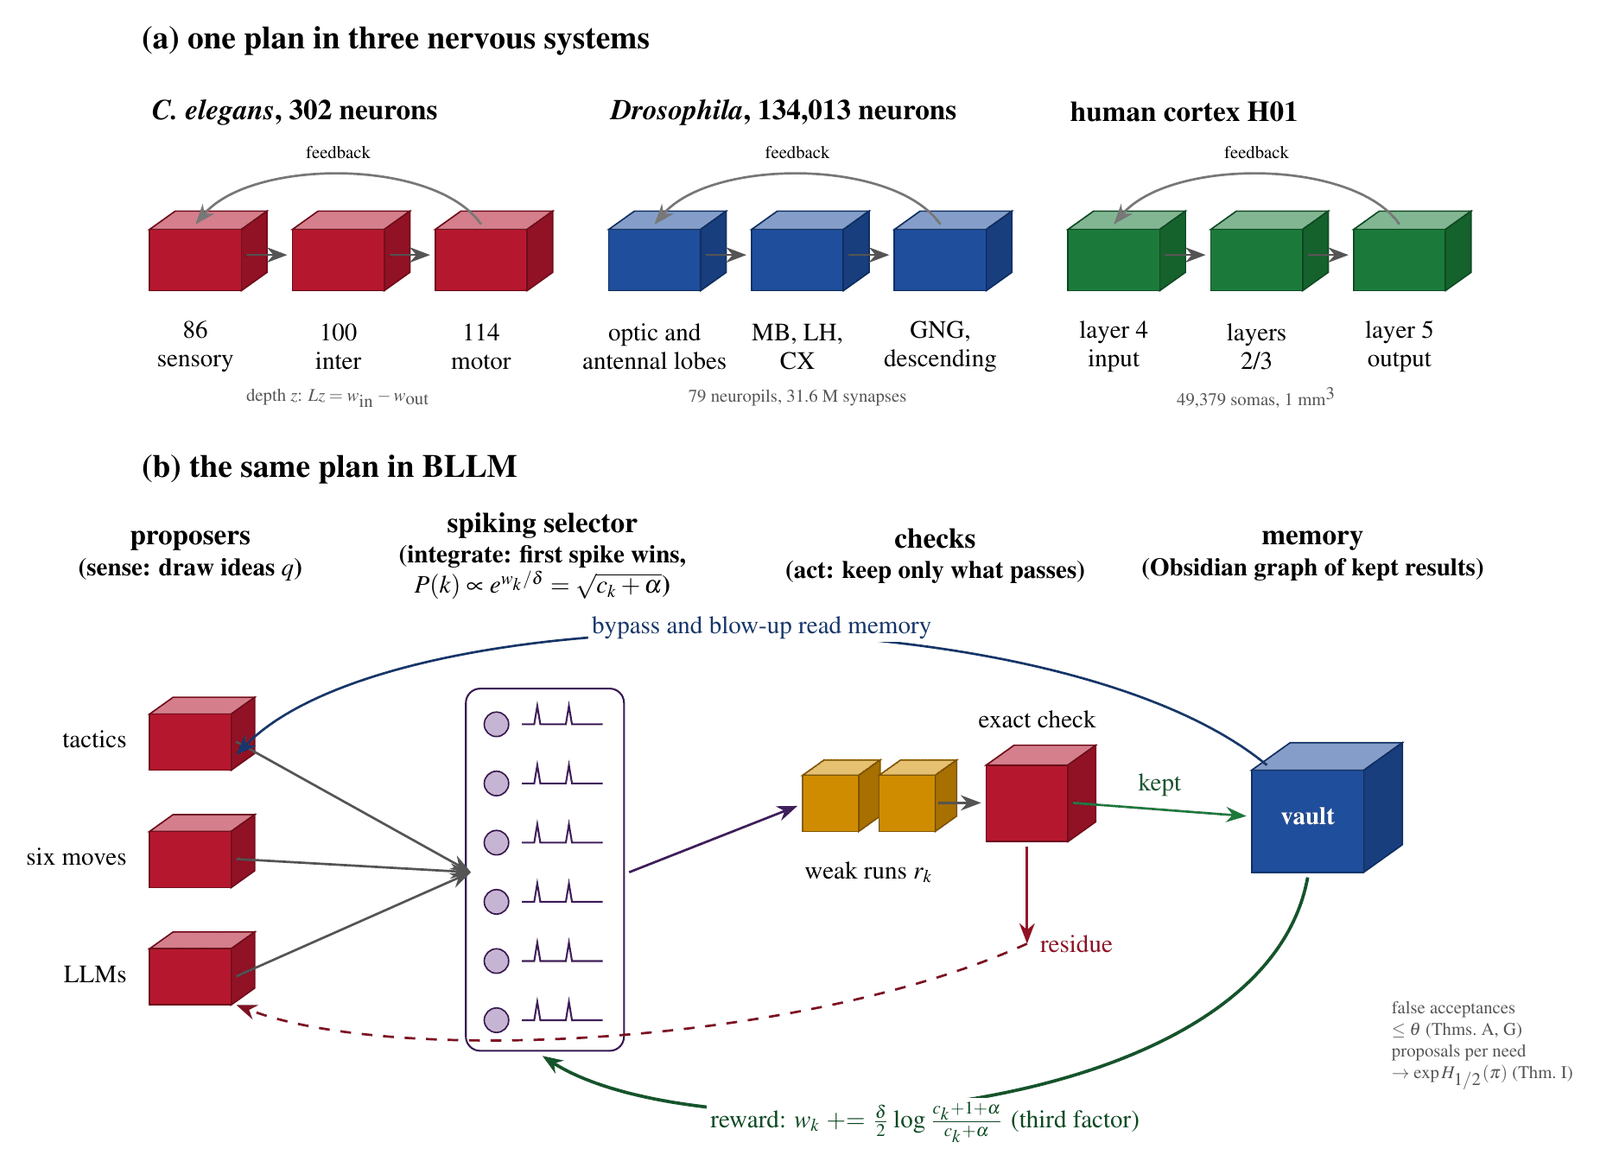
\includegraphics[width=0.98\textwidth]{figures/fig_brainmap}
\caption{One plan in three nervous systems and in a BLLM. (a) Sensory, integrating and output stages, with feedback, in the worm \cite{CJB19}, the fly \cite{DMS24b} and the human cortex \cite{SJB24}; the numbers are those of the reconstructions. (b) The same plan in a BLLM: proposers (language models, the six moves of Section~\ref{ssec:moves}, tactic search) draw ideas from a profile $q$; the spiking selector of Section~\ref{ssec:selector} chooses who proposes next by a race to the first spike; weak runs and one exact check keep only what passes (Theorem~\ref{thm:cascade}); kept results enter the memory, which bypass and blow-up read, and send the reward \eqref{eq:spikereward} back to the selector; rejected candidates leave residues for the proposers. The checks bound the expected number of false acceptances by $\theta$ (Theorems~\ref{thm:A} and~\ref{thm:G}), and the selector brings the number of proposals per need to $e^{H_{1/2}(\pi)}$ (Theorem~\ref{thm:I}).}
\label{fig:brainmap}
\end{figure*}

\subsection{The worm: depth of processing}

The hermaphrodite connectome has $448$ nodes, $300$ neurons and $148$ muscles and end organs, with $27{,}019$ chemical synapses in $4{,}681$ connections and $12{,}683$ gap-junction contacts in $2{,}698$. Varshney and coauthors gave its neurons a \emph{processing depth} \cite{VCP11}: a coordinate that increases along the direction in which signals travel. Let $W$ be the matrix of synaptic weights, $\mathrm{in}_{k}=\sum_{i}W_{ik}$ and $\mathrm{out}_{k}=\sum_{j}W_{kj}$, and let $L$ be the Laplacian of the symmetric matrix $(W+W^{\top})/2$.

\begin{lemma}[Processing depth]\label{lem:depth}
The system $Lz=\mathrm{in}-\mathrm{out}$ has a solution, unique up to an additive constant on each connected component, and it is the minimiser of $\sum_{i,j}W_{ij}(z_{j}-z_{i}-2)^{2}$.
\end{lemma}

\begin{proof}
The kernel of $L$ is spanned by the indicator vectors of the connected components, and $L$ is symmetric, so its range is the set of vectors that sum to zero on every component. Each synapse $i\to j$ adds $W_{ij}$ to $\mathrm{in}_{j}$ and to $\mathrm{out}_{i}$, both in the same component, so $\mathrm{in}-\mathrm{out}$ sums to zero there. For the variational form, $z^{\top}Lz=\frac12\sum_{i,j}W_{ij}(z_{j}-z_{i})^{2}$ and $(\mathrm{in}-\mathrm{out})^{\top}z=\sum_{i,j}W_{ij}(z_{j}-z_{i})$, so $\frac12z^{\top}Lz-(\mathrm{in}-\mathrm{out})^{\top}z=\frac14\sum_{i,j}W_{ij}(z_{j}-z_{i}-2)^{2}-\sum_{i,j}W_{ij}$, a convex function whose critical points are the solutions.
\end{proof}

So $z$ is the arrangement in which every synapse comes as close as possible to pointing two units deeper; with another normalisation of the Laplacian the unit changes and the order does not. Computed on the chemical and electrical synapses together, the mean depth is $-1.92$ for the $86$ sensory neurons, $-0.68$ for the $100$ interneurons, $-0.22$ for the $114$ motor neurons and $+1.75$ for the muscles. Four of the five shallowest neurons are amphid sensory neurons, AWAL, AWAR, ASIL and ASEL, and the deepest nodes are pharyngeal muscles and marginal cells. The order sensory, inter, motor, muscle is not imposed; it is computed from the wiring alone, and it is the order of the three stages of Fig.~\ref{fig:brainmap}(a). Figure~\ref{fig:worm} draws every node at its depth, against a spectral coordinate: the rank of the node in the lowest eigenvector of the normalised Laplacian that is spread over at least a quarter of the neurons, the third, with eigenvalue $0.123$.

\begin{figure*}[t]
\centering
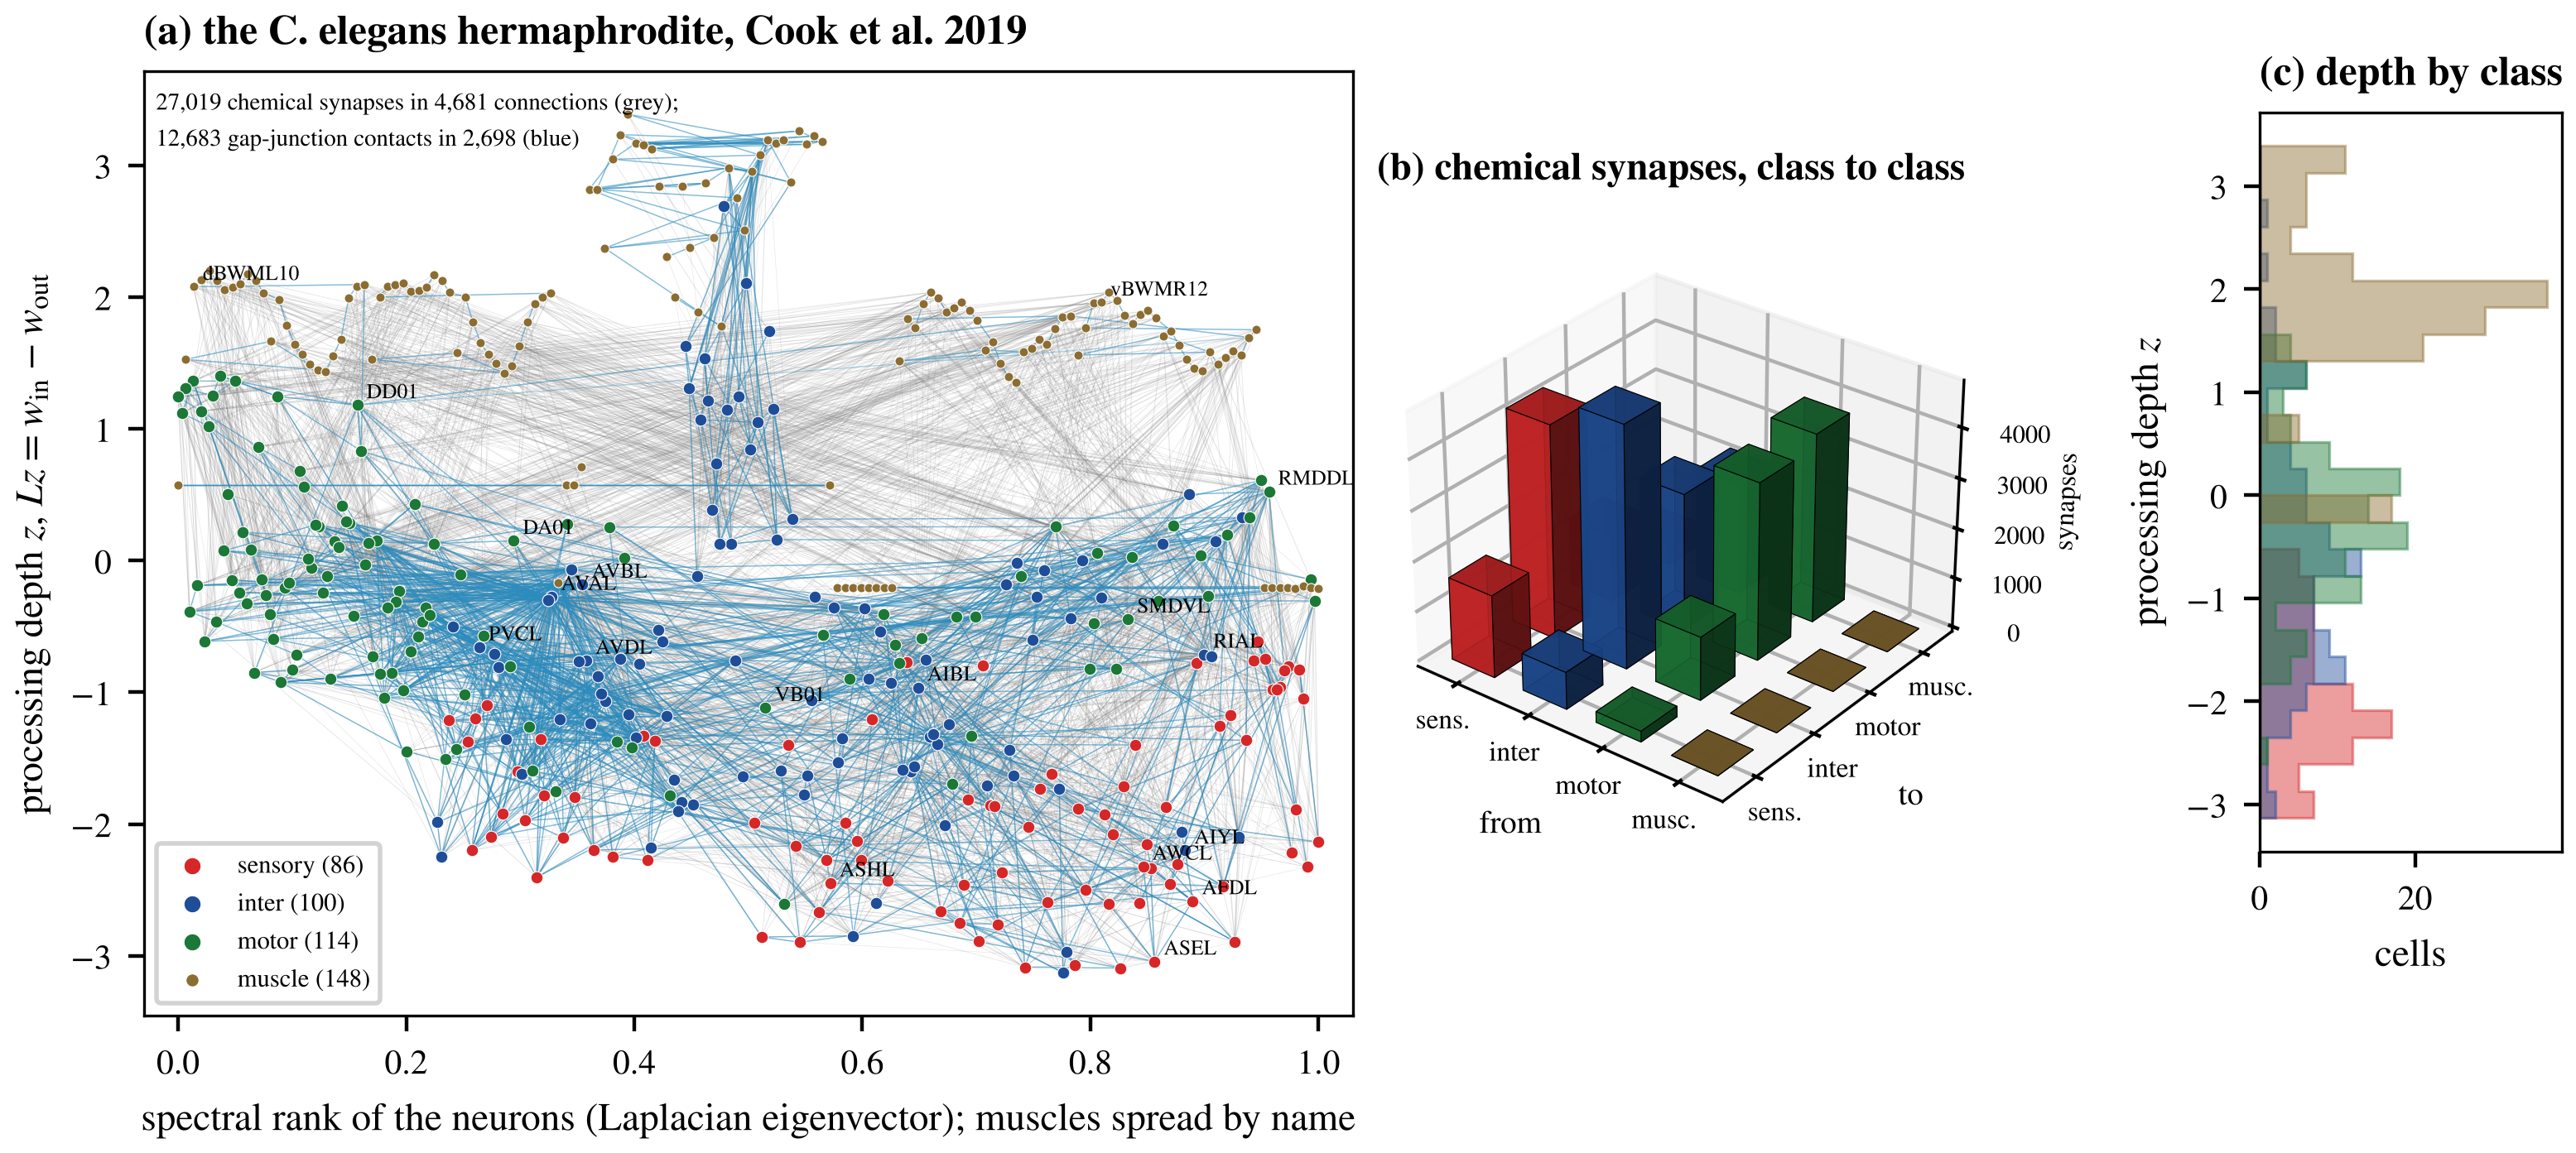
\includegraphics[width=0.98\textwidth]{figures/fig_worm}
\caption{The \textit{C.~elegans} hermaphrodite \cite{CJB19}. (a) Every neuron and muscle at its processing depth $z$ (Lemma~\ref{lem:depth}) against its rank in a spectral coordinate of the neurons, with chemical connections in grey and gap junctions in blue; muscles, which have no spectral coordinate, are spread by name. Sensory neurons lie lowest and muscles highest. (b) Chemical synapses from class to class: the largest flows are from sensory neurons to interneurons, from interneurons to interneurons and motor neurons, and from motor neurons to muscles. (c) The distribution of depths in each class.}
\label{fig:worm}
\end{figure*}

The package can also run this wiring. It builds an echo-state network whose recurrent matrix is the connectome itself, scaled to spectral radius $0.9$, with one sign per presynaptic neuron, as Dale's principle requires (excitatory with probability $0.8$, since the transmitter map of the worm is not part of the wiring data), and fits a linear readout \cite{JH04}. Its short-term memory, the squared correlation between the input $k$ steps back and its best linear readout from sixty units, is $0.77$, $0.37$, $0.27$ and $0.14$ for $k=1,2,4,8$. This makes no claim that a worm-shaped reservoir computes better than another; it lets the memory and the selector of a BLLM be wired as a real circuit, which is what the experiments of Lappalainen and coauthors show to be informative in the fly, where networks constrained by the connectome predict the activity of the visual system neuron by neuron \cite{LTP24}.

\subsection{The fly: 79 neuropils}

At a threshold of five synapses per connection the FlyWire brain has $134{,}013$ neurons, $2{,}710{,}038$ connections and $31{,}578{,}726$ synapses in $79$ neuropils. Give each neuron the neuropil where it receives most of its input, and count every synapse from the neuropil of its presynaptic neuron to the neuropil where it lies. The resulting matrix (Fig.~\ref{fig:fly}(a)) has $59.0\%$ of its weight on the diagonal: most synapses are made where the presynaptic neuron itself listens, a local and recurrent integration. The off-diagonal weight connects the stages of Fig.~\ref{fig:brainmap}(a): the optic lobes and antennal lobes, which receive the senses, project to the mushroom bodies, the lateral horn and the central complex, which integrate and learn, and these to the premotor neuropils and the gnathal ganglion, where the descending neurons leave for the body. Acetylcholine, excitatory in the fly, is the predicted transmitter of $57.1\%$ of the synapses, GABA of $24.7\%$ and glutamate, mostly inhibitory, of $16.4\%$; serotonin, dopamine and octopamine together of $1.8\%$, concentrated in the mushroom bodies where dopamine carries the reward signal of associative learning. The numbers of partners are heavy-tailed: the median neuron has $11$ output partners and $10$ input partners, the mean about $19$, and the largest $6{,}398$ and $5{,}066$ (Fig.~\ref{fig:fly}(c)).

\begin{figure*}[t]
\centering
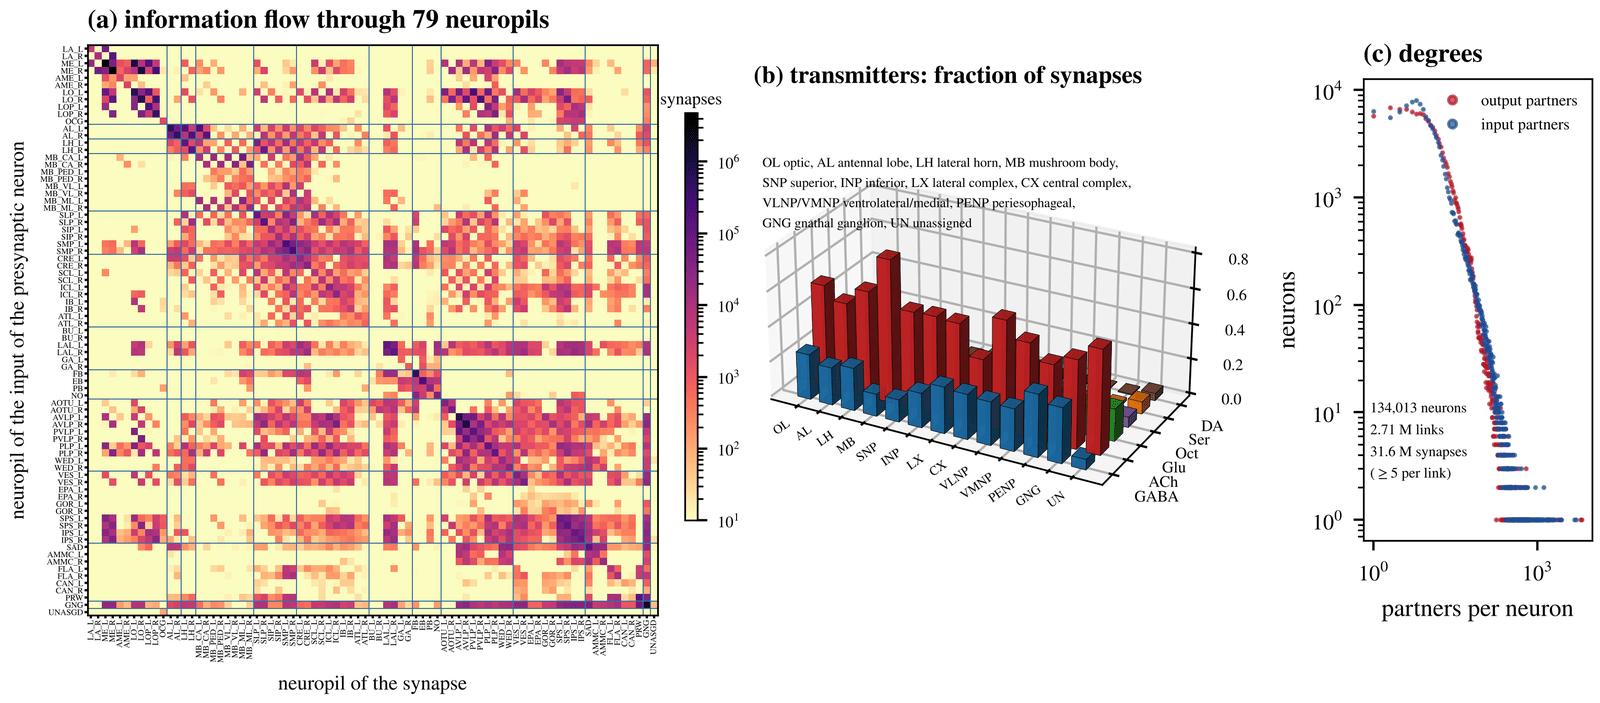
\includegraphics[width=0.98\textwidth]{figures/fig_fly}
\caption{The adult \textit{Drosophila} brain, FlyWire release 783, connections of at least five synapses \cite{DMS24b}. (a) Synapses from the neuropil where the presynaptic neuron receives most of its input (rows) to the neuropil of the synapse (columns), on a logarithmic scale, with the neuropils grouped into the super-groups of FlyWire; $59\%$ of the weight is on the diagonal. (b) The predicted transmitter of the synapses \cite{EBC24} in each super-group. (c) The numbers of output and input partners per neuron.}
\label{fig:fly}
\end{figure*}

\subsection{The human cortex: six layers}

H01 is a fragment of human temporal cortex of about a cubic millimetre, reconstructed by electron microscopy at nanometre resolution \cite{SJB24}. Its table of somas lists $49{,}379$ cells: $20{,}139$ oligodendrocytes, $8{,}803$ pyramidal neurons, $6{,}536$ microglia and precursor cells, $5{,}474$ astrocytes and $4{,}688$ interneurons, among others, with $16{,}253$ neurons in all. The layers are its stages (Fig.~\ref{fig:cortex}). Layer~1 holds almost no neurons ($2\%$ of its cells are pyramidal); pyramidal neurons are $40\%$ of the cells of layer~2, $25\%$ of layer~3, $33\%$ of layer~4, $18\%$ of layer~5 and $16\%$ of layer~6, interneurons are densest in layer~2 ($24\%$), and the white matter below is $77\%$ oligodendrocytes, the insulation of the axons that leave. In the canonical circuit of the neocortex \cite{DM04}, input from the thalamus arrives in layer~4, is integrated in the recurrent networks of layers~2 and~3, and leaves from the large pyramidal neurons of layer~5, with feedback from layer~6 to the thalamus: the plan of Fig.~\ref{fig:brainmap}(a) again.

\begin{figure*}[t]
\centering
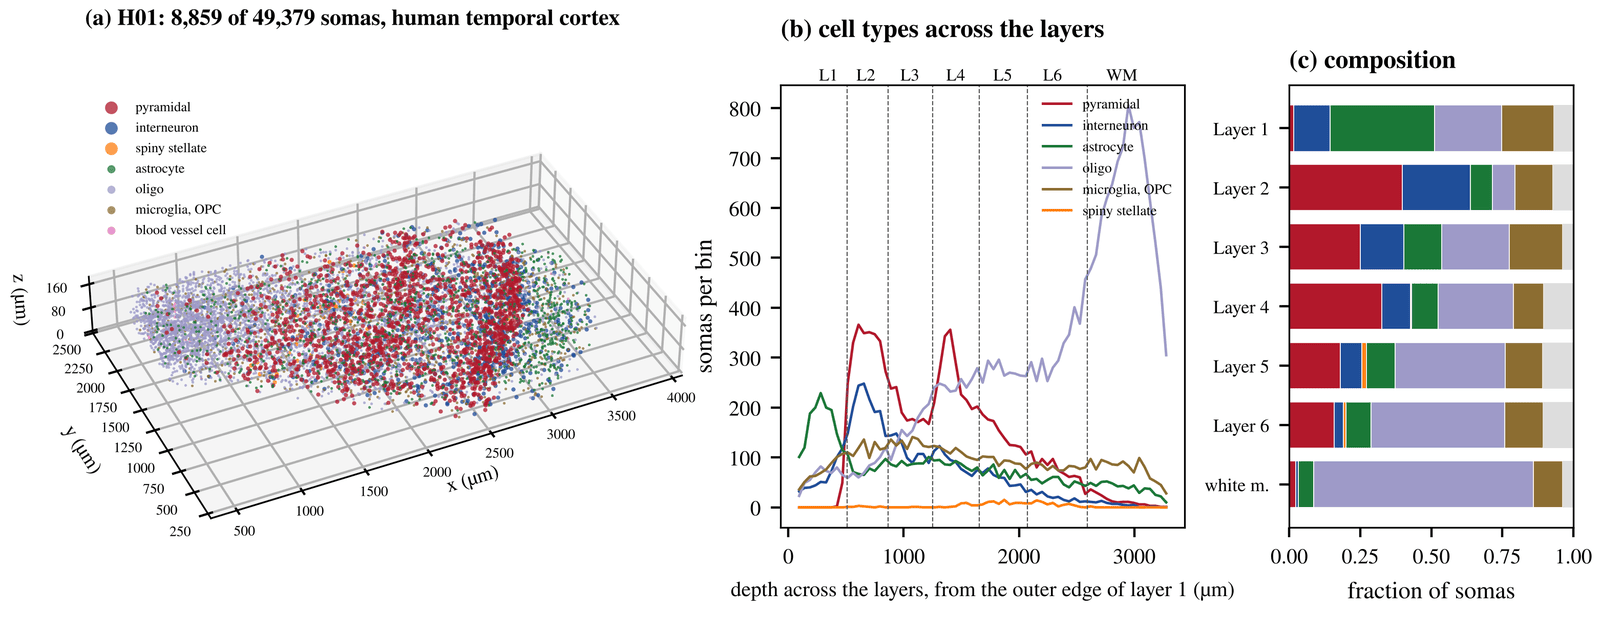
\includegraphics[width=0.98\textwidth]{figures/fig_cortex}
\caption{The human cortical fragment H01 \cite{SJB24}. (a) A random sample of $8{,}859$ of its $49{,}379$ somas at their positions, coloured by cell type. (b) The number of somas of each type along the axis of the layers, measured from the outer edge of layer~1, with the boundaries between layers. (c) The composition of each layer and of the white matter.}
\label{fig:cortex}
\end{figure*}

\subsection{From wiring to a BLLM}

The three stages carry over with a precise meaning. The \emph{sensing} stage is the set of proposers, whose profile $q$ is what Theorem~\ref{thm:I} measures. The \emph{integrating} stage is the selector, whose job, like that of the basal ganglia in the account of Redgrave, Prescott and Gurney \cite{RPG99}, is to choose one action among competing ones and to learn from a reward signal which choices pay, the role that dopamine plays in the account of Schultz, Dayan and Montague \cite{SDM97}; Proposition~\ref{prop:spiking} shows that with a race to the first spike this choice is square-root sampling, the optimum of the gap law. The \emph{acting} stage is the cascade of checks, which lets through only what passes, and the \emph{feedback} is the memory and the residues. One part of the plan of a brain has no counterpart: no stage of a nervous system certifies what it keeps, and that is the part this paper adds. A BLLM is therefore not a model of a brain. It is a system that keeps the organisation which brains share, replaces the stage that decides by a check whose cost is priced by Theorems~\ref{thm:A} to~\ref{thm:H}, and uses at the stage of choice the mechanism that the gap law shows to be optimal. Because the selector is a circuit of leaky integrate-and-fire neurons with a local learning rule, it can run on neuromorphic hardware \cite{Mea90,DSL18}; we have run it only in simulation.

\section{Growth laws and the price of a sound takeoff}\label{sec:scaling}

\subsection{Osgood takeoffs}

Theorems~\ref{thm:E} and~\ref{thm:F} take the costs $a_{n}$ as given. Growth models of an intelligence explosion produce them. The simplest such model, and the one behind most informal arguments, is the equation
\[
\frac{dI}{dt}=c\,I^{\alpha},\qquad c>0,\ \alpha>0,
\]
for a capability $I$ that speeds up its own improvement. Its solution from $I(0)=1$ reaches infinity at the finite time $\int_{1}^{\infty}dI/(cI^{\alpha})=1/(c(\alpha-1))$ when $\alpha>1$ and grows without blowing up when $\alpha\le1$; Osgood's criterion states the same for $dI/dt=f(I)$ with the integral of $1/f$ \cite{Osg98}.\footnote{W.~F. Osgood, \emph{Beweis der Existenz einer L\"osung der Differentialgleichung $dy/dx=f(x,y)$ ohne Hinzunahme der Cauchy--Lipschitzschen Bedingung}, Monatshefte f\"ur Mathematik und Physik 9 (1898), 331--345 \cite{Osg98}. The paper is about uniqueness; the blow-up criterion that bears Osgood's name is the elementary fact, implicit there, that a solution of $y'=f(y)$ with $f>0$ reaches infinity in the finite time $\int_{y_{0}}^{\infty}dy/f(y)$ exactly when the integral converges. For $f(y)=cy^{\alpha}$ the integral is $y_{0}^{1-\alpha}/(c(\alpha-1))$ for $\alpha>1$ and diverges for $\alpha\le1$.} To put a check on the curve one has to say what one improvement is. Two choices are natural.

\emph{Additive steps.} The $n$-th improvement raises the capability from $n$ to $n+1$ at the rate reached at its start, so it takes the time $g_{n}=1/(cn^{\alpha})$.

\emph{Multiplicative steps.} The $n$-th improvement multiplies the capability by a fixed factor $\lambda>1$, from $\lambda^{n-1}$ to $\lambda^{n}$, at the rate reached at its start, so it takes the time $g_{n}=(\lambda-1)\lambda^{n-1}/(c\lambda^{(n-1)\alpha})=\frac{\lambda-1}{c}\,q^{n-1}$ with $q=\lambda^{-(\alpha-1)}$.

In both cases we let the check of the $n$-th improvement cost a fixed fraction $\kappa>0$ of the time it took to make, $a_{n}=\kappa g_{n}$ per run, so that faster improvements are also faster to check. Write $G=\sum_{n}g_{n}$ for the unchecked takeoff time and $T_{\theta}=G+\Vs(\theta)$ for the least time of a takeoff with at most $\theta$ expected false acceptances, measured, as in Theorem~\ref{thm:A}, in the run in which every candidate is correct.

\begin{proposition}[Osgood takeoffs]\label{prop:osgood}
Let $\alpha>1$, $0<\theta\le1$ and $0<\eps<1$.
\begin{enumerate}[label=\textup{(\roman*)},leftmargin=2.2em,itemsep=1pt]
\item In both models
\[
\begin{aligned}
\frac{T_{\theta}}{G}&\ge 1+\frac{\kappa}{L}\Bigl(H+\log\frac1\theta\Bigr),\\
\frac{T_{\theta}}{G}&\le 1+\frac{\kappa}{L}\Bigl(H+\log\frac1\theta\Bigr)+\kappa ,
\end{aligned}
\]
where $H$ is the entropy of the profile $g/G$.
\item For additive steps $G=\zeta(\alpha)/c$, which lies between $1/(c(\alpha-1))$ and $\alpha/(c(\alpha-1))$, and, as $\alpha\to1^{+}$,
\[
H=\frac1{\alpha-1}+\log\frac1{\alpha-1}+O(1).
\]
Hence the least check time of a sound takeoff is
\[
T_{\theta}-G=\frac{\kappa\bigl(1+O\bigl((\alpha-1)\log\frac1{\alpha-1}\bigr)\bigr)}{c(\alpha-1)^{2}L}.
\]
\item For multiplicative steps $G=(\lambda-1)/(c(1-q))$ and
\[
\begin{aligned}
H&=\log\frac1{1-q}+\frac{q}{1-q}\log\frac1q\\
&=\log\frac1{(\alpha-1)\log\lambda}+1+o(1)\qquad(\alpha\to1^{+}).
\end{aligned}
\]
Hence
\[
T_{\theta}-G=\frac{\kappa}{c(\alpha-1)L}\cdot\frac{\lambda-1}{\log\lambda}\Bigl(\log\frac1{\alpha-1}+O(1)\Bigr).
\]
\item With checks of polynomial order $s$, a sound takeoff of finite cost exists for additive steps if and only if $\alpha>1+s$, and then its least check cost is $\frac{\kappa}{c}\,\theta^{-s}\zeta\bigl(\frac{\alpha}{1+s}\bigr)^{1+s}$; for multiplicative steps it exists for every $s>0$, with least check cost $\kappa G\,\theta^{-s}(1-q)/(1-q^{1/(1+s)})^{1+s}$.
\end{enumerate}
\end{proposition}

\begin{proof}
(i) The profile of the checks is $a/A=g/G$ and $A=\kappa G$. Proposition~\ref{prop:infinite} gives $\frac AL(H+\log\frac1\theta)\le\Vs(\theta)\le\frac AL(H+\log\frac1\theta)+A$; divide by $G$.

(ii) $G=\sum_{n}n^{-\alpha}/c=\zeta(\alpha)/c$, and $1/(\alpha-1)\le\zeta(\alpha)\le1+1/(\alpha-1)$ by comparison with the integral, as in the proof of Proposition~\ref{prop:powerlaw}, which also gives the expansion of $H$. Then $T_{\theta}-G=\kappa G\,(H+\log\frac1\theta+O(L))/L$ by (i), and $\kappa G H=\frac{\kappa}{c}\bigl(\frac1{\alpha-1}+O(1)\bigr)\bigl(\frac1{\alpha-1}+O(\log\frac1{\alpha-1})\bigr)$.

(iii) $G=\frac{\lambda-1}{c}\sum_{n\ge1}q^{n-1}=\frac{\lambda-1}{c(1-q)}$. The profile is geometric, $p_{n}=(1-q)q^{n-1}$, so $\log(1/p_{n})=\log\frac1{1-q}+(n-1)\log\frac1q$ and $\sum_{n}(n-1)p_{n}=q/(1-q)$; this is the formula for $H$. As $\alpha\to1^{+}$, $u=(\alpha-1)\log\lambda\to0$ and $q=e^{-u}$, so $1-q=u+O(u^{2})$ and $\frac{q}{1-q}\log\frac1q=\frac{ue^{-u}}{1-e^{-u}}\to1$; and $G=\frac{\lambda-1}{c\,u}(1+O(u))$. Combine with (i).

(iv) By Corollary~\ref{cor:dualcases}(ii) a sound allocation of finite cost exists if and only if $\sum_{n}a_{n}^{1/(1+s)}<\infty$. For additive steps this is $\sum n^{-\alpha/(1+s)}<\infty$, that is $\alpha>1+s$; for multiplicative steps it is a geometric series. For the value, let $\beta=1/(1+s)$ and $S=\sum_{n}a_{n}^{\beta}<\infty$. For every allocation with $\sum_{n}\delta_{n}\le\theta$ and every $N$, the lower bound in the proof of Theorem~\ref{thm:D}, applied to the first $N$ checks, gives $\sum_{n\le N}a_{n}\delta_{n}^{-s}\ge\theta^{-s}(\sum_{n\le N}a_{n}^{\beta})^{1+s}$; letting $N\to\infty$, every sound allocation costs at least $\theta^{-s}S^{1+s}$, and the allocation $\delta_{n}=\theta a_{n}^{\beta}/S$ attains it, by the computation of the attainment step there. For additive steps $S=(\kappa/c)^{\beta}\zeta(\alpha\beta)$, and for multiplicative steps $S=A^{\beta}\sum_{n}p_{n}^{\beta}=A^{\beta}(1-q)^{\beta}/(1-q^{\beta})$, with $A=\kappa G$.
\end{proof}

So the takeoff can be made sound whenever it is singular, and the price is the factor $\frac\kappa L(H+\log\frac1\theta)$ on the time. Near the critical exponent the two counts of improvements part ways (Fig.~\ref{fig:takeoff}). If every unit of capability is a separate modification that must be checked, the entropy of the profile is of order $1/(\alpha-1)$, and the checks cost a factor $1/(\alpha-1)$ more than the improvements, $\kappa/(c(\alpha-1)^{2}L)$ in all. If every doubling of capability is one modification, the entropy is only $\log\frac1{\alpha-1}$. At $\alpha=1.01$, $\eps=\frac12$ and $\theta=10^{-6}$ the lower bound of (i) gives a slowdown factor $1+171.5\,\kappa$ for additive steps and $1+28.6\,\kappa$ for doublings; at $\alpha=2$ the two factors are $1+22.3\,\kappa$ and $1+21.9\,\kappa$, and the budget term $\log_{2}10^{6}\approx19.9$ dominates. With Chebyshev checks, $s=1$, additive steps need $\alpha>2$, and at $\alpha=3$ the least check cost is $\frac\kappa c\,\zeta(\frac32)^{2}\cdot10^{6}\approx6.8\times10^{6}\,\frac\kappa c$, five orders of magnitude above the $25.1\,\frac\kappa c$ of exponential checks.

\begin{figure*}[t]
\centering
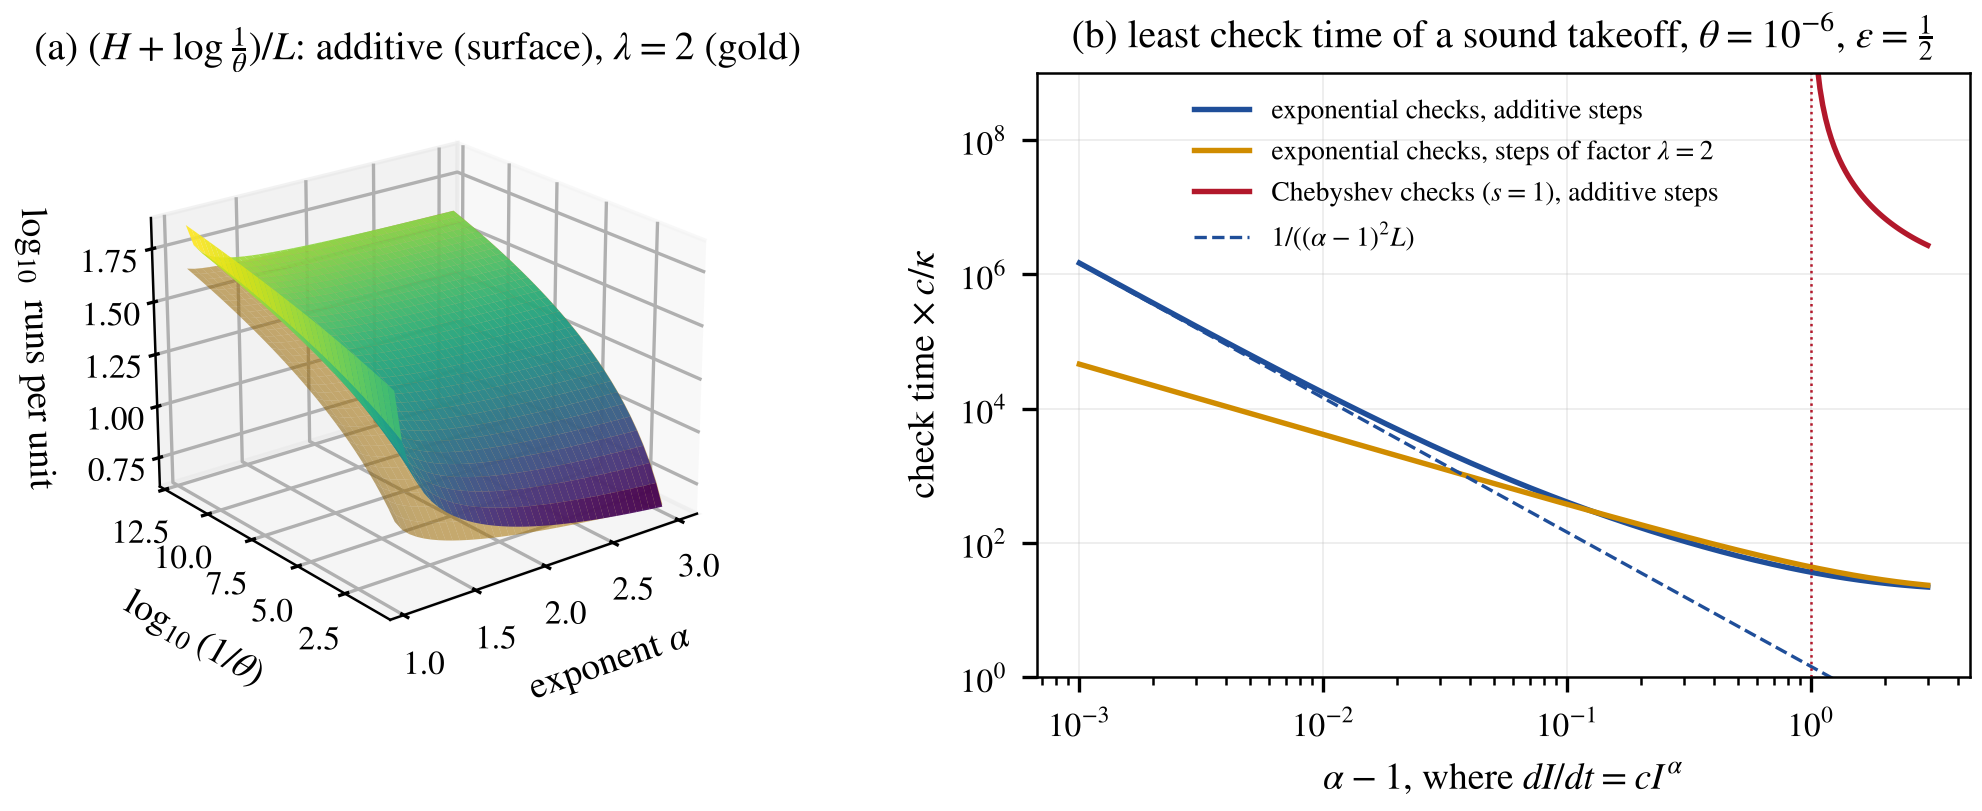
\includegraphics[width=0.98\textwidth]{figures/fig_takeoff}
\caption{Proposition~\ref{prop:osgood}, with $\eps=\frac12$. (a) The lower bound $(H+\log\frac1\theta)/L$ for the number of runs per unit of check cost, on a logarithmic scale, as a function of the growth exponent $\alpha$ and of $\log_{10}(1/\theta)$, for additive steps (coloured surface) and for doublings, $\lambda=2$ (gold surface). The additive surface rises like $1/(\alpha-1)$ as $\alpha\to1$, the multiplicative one like $\log\frac1{\alpha-1}$. (b) The lower bound for the least check time of a sound takeoff, in units of $\kappa/c$, at $\theta=10^{-6}$, against $\alpha-1$ on logarithmic axes: exponential checks with additive steps (blue), which approach $1/((\alpha-1)^{2}L)$ (dashed), exponential checks with doublings (gold), and Chebyshev checks with additive steps (red), which cost infinitely much for $\alpha\le2$ (dotted line).}
\label{fig:takeoff}
\end{figure*}

\subsection{What the growth exponent is, and what it is not}

The exponent $\alpha$ of Proposition~\ref{prop:osgood} is the elasticity of the speed of research with respect to the capability of the system that does it. It is not one of the exponents of the empirical scaling laws of language models. Kaplan and coauthors fitted the test loss of a language model trained with the optimal allocation of a compute budget $C$ to a power law $C^{-\alpha_{C}}$ with $\alpha_{C}\approx0.050$ \cite{KMH20}, and Hoffmann and coauthors fitted the loss as $E+A_{0}N^{-0.34}+B_{0}D^{-0.28}$ in the number $N$ of parameters and the number $D$ of training tokens \cite{HBM22}.\footnote{J.~Kaplan, S.~McCandlish, T.~Henighan, T.~B. Brown, B.~Chess, R.~Child, S.~Gray, A.~Radford, J.~Wu and D.~Amodei, \emph{Scaling laws for neural language models}, arXiv:2001.08361 (2020) \cite{KMH20}; J.~Hoffmann et~al., \emph{Training compute-optimal large language models}, arXiv:2203.15556 (2022) \cite{HBM22}. Both fits measure the cross-entropy loss on held-out text. The exponent $\alpha_{C}\approx0.050$ is that of the compute-efficient frontier in the first paper; the exponents $0.34$ and $0.28$, with fitted constants $E\approx1.69$, $A_{0}\approx406.4$ and $B_{0}\approx410.7$, are those of the parametric fit of the second. The letters $A_{0}$ and $B_{0}$ are renamed here to avoid a clash with the total cost $A$.} These laws relate loss to resources. To turn them into a value of $\alpha$ one needs two further maps, from loss to research ability and from research ability to the speed of the next improvement, and neither has been measured. Anbar Jafari, Ozcinar and Anbarjafari propose to estimate how fast improvement accelerates relative to its current level from series that engineers already record, which is an estimate of $\alpha$ \cite{AOA25}; the phase transitions and predictability limits of the first author with Singha Roy and Samal are a second approach to the same question \cite{BSS26}.

Ord observes that a singular growth path needs the generation time, the time around the loop of improvement, to tend to zero \cite{Ord26}. In the present model this is the condition $g_{n}\to0$, which a convergent $\sum g_{n}$ forces. Theorem~\ref{thm:E} adds a second clock: the time spent checking the $n$-th improvement must also tend to zero, and faster than the generation time can afford to, because the sum of $a_{n}\log(1/a_{n})$, and not only of $a_{n}$, must converge. Proposition~\ref{prop:osgood} shows that for power laws this second condition is free in kind and expensive in amount: every Osgood takeoff with $\alpha>1$ can be made sound with exponential checks, but near the threshold the checks take longer than the improvements by a factor that diverges as $1/(\alpha-1)$ when every unit of capability is checked. With checks that are only polynomially reliable, the threshold for a sound takeoff moves from $\alpha=1$ to $\alpha=1+s$, and between the two lies a range of singular takeoffs that cannot be made sound at any cost.

\begin{remark}[Errors of the generator]
Proposition~\ref{prop:osgood} prices the run in which every candidate is correct. If the $n$-th candidate is incorrect with probability in $[\rho_{\ast},\bar\rho]\subset(0,1)$ and incorrect candidates are regenerated, the proof of Theorem~\ref{thm:B}, with Proposition~\ref{prop:infinite} in place of Theorem~\ref{thm:A}, applies to the infinite chain: the lower bound holds with $\theta$ replaced by $\theta/\rho_{\ast}$, and the upper bound with $\theta$ replaced by $\theta(1-\bar\rho)/\bar\rho$ and the whole multiplied by $1/(1-\bar\rho)$. The orders in $\alpha-1$ of parts (ii) and (iii) do not change.
\end{remark}

\section{Formal proofs of hard problems}\label{sec:cases}

Several of the hardest problems of mathematics now have proofs that a machine has checked line by line, and four of these formal proofs were written with the help of artificial intelligence \cite{Ant26,ZDC26,HBL26,OAI26}. They are the natural test of the theory: each is a long chain of steps, each step has a check, and each records which steps were hard. This section reads six of them in the language of Sections~\ref{sec:chains} and~\ref{sec:agents}, states what a BLLM adds and what it does not, and describes the package that implements the system.

\subsection{Six problems}

\begin{figure*}[t]
\centering
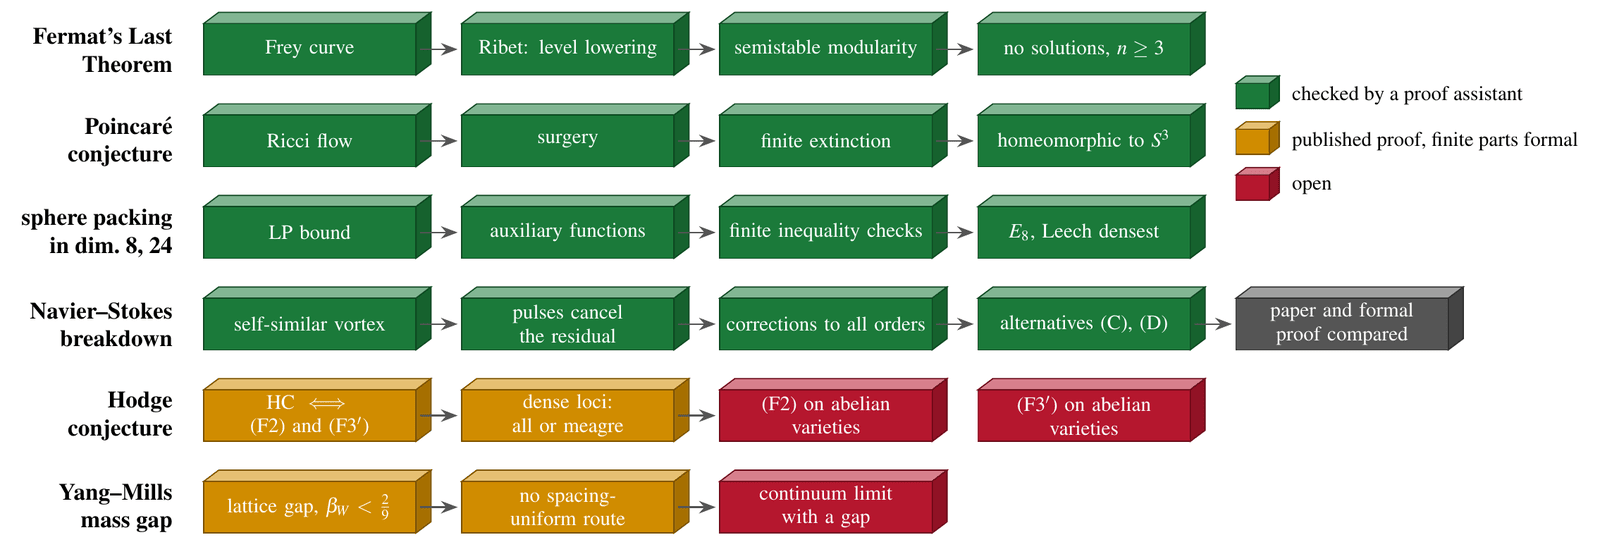
\includegraphics[width=0.98\textwidth]{figures/fig_cases}
\caption{The main steps of the six proofs of Table~\ref{tab:cases}. Green steps are checked by a proof assistant, gold steps have published proofs whose formal checks cover only finite parts, red steps are open, and grey marks the comparison of the Navier--Stokes paper with its formal proof \cite{BCH26}. The two Hodge statements (F2) and (F3$'$) are independent, and both are needed.}
\label{fig:cases}
\end{figure*}

Table~\ref{tab:cases} and Fig.~\ref{fig:cases} list the problems, the formal results and the steps that remain. Four are settled: Fermat's Last Theorem by Wiles and by Taylor and Wiles \cite{Wil95,TW95}, formalised in Lean~4 in September 2026 by dozens of Claude agents in eleven days on the Prove2Me platform, along the simplified proof of Darmon, Diamond and Taylor, in about thirteen million lines with $29{,}500$ theorems in the final proof and only the three standard axioms \cite{Ant26,CML26,DDT95}; the Poincar\'e conjecture by Perelman, now formalised in Lean~4 with Mathlib following the account of Morgan and Tian \cite{ZDC26}; the sphere packing problem in dimensions $8$ and $24$ \cite{Via17,CKM17}, formalised by Hariharan, Birkbeck, Lee, Ma, Mehta, Poiroux and Viazovska and completed by Math, Inc. \cite{HBL26}; and finite-time breakdown of the three-dimensional Navier--Stokes equations with forcing, alternatives (C) and (D) of the official description of the Millennium problem, proved by OpenAI for every positive viscosity in a paper of 165 pages and in Lean \cite{OAI26}. Each formal development is archived with a record of an independent build \cite{ArcNS,ArcPC,ArcSP}. Two are open: the Hodge conjecture, which the first two authors reduced to two statements (F2) and (F3$'$) about abelian varieties \cite{BB26c}, and the existence of Yang--Mills theory with a mass gap, for which they proved a lattice mass gap for four-dimensional $\mathrm{SU}(2)$ up to the coupling $\beta_{W}=\frac29$, the limit of single-link Dobrushin arguments \cite{BB26d}.\footnote{D.~Bhattacharjee and U.~Bhattacharya, \emph{Dense algebraic loci of Hodge classes}, Hexagon preprint hexagon:2610.00315v1 (17 October 2026), with Lean~4 archive doi:10.5281/zenodo.23439578 \cite{BB26c}. The paper proves that the Hodge conjecture is equivalent to two statements about abelian varieties, that the locus on which either holds is dense in every family and is either the whole family or a meagre set, builds for each statement the object it needs next and proves at which step it stops. The second work, \emph{Lattice Yang--Mills theory: spacing-uniform obstructions, the mass gap up to the Dobrushin ceiling, and Lean certificate}, Zenodo (2026), doi:10.5281/zenodo.23449466 \cite{BB26d}, also proves that lattice inequalities uniform in the spacing cannot produce the continuum mass gap, and isolates the remaining step as one hypothesis on the ratio of the lattice gap to the spacing.}

\begin{table*}[t]
\caption{Six problems with machine-checked or published proofs, in the language of the moves of Section~\ref{ssec:moves}. ``Formal'' names the proof checker of the archived development; the last column names the moves on which the proof rests.}
\label{tab:cases}
\centering
\footnotesize
\setlength{\tabcolsep}{4pt}
\begin{tabular}{@{}p{0.13\textwidth}p{0.29\textwidth}p{0.08\textwidth}p{0.24\textwidth}p{0.17\textwidth}@{}}
\toprule
Problem & What is proved & Formal & What remains & Moves \\
\midrule
\rr Fermat's Last Theorem & \rr modularity of semistable elliptic curves, hence the theorem \cite{Wil95,TW95,Ant26} & Lean~4 & \rr nothing & \rr bypass (Frey, Ribet), residual (Taylor--Wiles) \\
\rr Poincar\'e conjecture & \rr Hamilton--Perelman Ricci flow with surgery \cite{ZDC26} & Lean~4 & \rr nothing & \rr construction, residual (surgery) \\
\rr Sphere packing in dimensions 8, 24 & \rr $E_{8}$ and the Leech lattice are densest \cite{Via17,CKM17,HBL26} & Lean~4 & \rr nothing in dimensions 8, 24 & \rr construction, trivialization \\
\rr Navier--Stokes breakdown & \rr alternatives (C), (D) for every viscosity \cite{OAI26} & Lean~4 & \rr the correspondence of paper and formal proof \cite{BCH26} & \rr construction, residual, blow-up \\
\rr Hodge conjecture & \rr equivalence with (F2) and (F3$'$); dense loci \cite{BB26c} & \rr Lean~4, finite parts & \rr (F2), (F3$'$) & \rr bypass, strong then weak \\
\rr Yang--Mills mass gap & \rr lattice gap for $\beta_{W}<\frac29$; no spacing-uniform route \cite{BB26d} & \rr Lean~4, finite parts & \rr continuum limit with a gap & \rr construction, strong then weak, residual \\
\bottomrule
\end{tabular}
\end{table*}

The history of the problems contains the moves of Section~\ref{ssec:moves}. Wiles announced a proof in 1993 in which one step failed; the repair with Taylor replaced it by a different argument \cite{TW95}, a residual move on a single step of a long chain. The Navier--Stokes construction of \cite{OAI26} builds a self-similar vortex, cancels the singular part of its momentum residual by oscillatory pulses and corrects what is left to every order: construction, residual and blow-up in one argument. The sphere packing proofs reduce optimality to the existence of auxiliary functions whose inequalities are checked by finite computations, a trivialization. The Hodge reduction replaces the conjecture by statements on abelian varieties through known theorems, a bypass, and weakens one of them to (F3$'$), a step down the ladder of strong then weak.

\subsection{What a BLLM adds, and what it does not}

Three of the theorems of this paper speak directly to these proofs.

First, Theorem~\ref{thm:gating}. A formal development checks every step of the formal argument, not the steps of the paper it formalises. Bastounis, Circelli and Hansen argue that the Lean proof of \cite{OAI26} does not follow the argument of the paper, and that a faithful translation of a natural-language proof is not computable in general \cite{BCH26}. Whatever the outcome of that discussion, a natural-language argument whose only certificate is a formal proof of its final statement is checked at its outcome, and Theorem~\ref{thm:gating} shows that certification at the outcome is exponentially more expensive in the number of steps than certification step by step. A BLLM that keeps the paper and the formal proof aligned keeps a check at every step of both.

Second, Theorem~\ref{thm:cascade}. The developments above contain tens of thousands of formal lemmas, and the strong check, a full build, is expensive. A system that proposes most steps wrongly and filters them with cheap checks pays the build essentially only on its correct proposals, with a premium logarithmic in the ratio of costs; this is what makes very large numbers of machine proposals affordable without any loss of soundness.

Third, Theorem~\ref{thm:G} and Corollary~\ref{cor:onlinesing}. A system that keeps working on an open problem does not know how many steps it will take or what they will cost. The online law lets it run indefinitely with a guaranteed bound on the expected number of false acceptances over its whole life, at a cost within a double logarithm of the best schedule chosen with hindsight.

What the theorems do not give is the step that no proposer produces. The open entries of Table~\ref{tab:cases}, (F2), (F3$'$) and the continuum limit with a gap, are statements for which no proof has been proposed, by people or by machines. A BLLM cannot make them easier to prove: its guarantee is that whatever it keeps has been checked, at the least possible cost, and that its record of what failed, the residues, is complete. That record is the part of the work a later proposer, human or artificial, can build on.

\subsection{Five strategies of mathematicians as proposers}\label{ssec:strategies}

The six moves of Section~\ref{ssec:moves} describe what a step does. The proofs above also show five larger strategies, each a way of choosing what to propose, and the package implements each of them as a proposer whose candidates meet the same checks.
\begin{enumerate}[label=(\roman*),leftmargin=1.8em,itemsep=1pt]
\item \emph{Certificate first} (Cohn and Elkies, Viazovska). Replace the statement by the existence of one explicit object whose properties imply it: Cohn and Elkies reduced the optimality of a sphere packing to an auxiliary function with sign conditions on it and on its Fourier transform \cite{CE03}, and Viazovska built that function in dimension~$8$ from quasimodular and weakly holomorphic modular forms, after which the sign conditions are finite inequalities \cite{Via17,CKM17}; the Lean development checks them \cite{HBL26,ArcSP}. The proposer searches a structured space for the certificate and hands the finite inequalities to the checks.
\item \emph{Flow with surgery} (Perelman). Evolve the object by a monotone flow, classify the limits at its singularities and cut them out \cite{Per02,Per03a,Per03b}. On a lattice gauge theory the corresponding flow is the gradient flow of the Wilson action \cite{Lus10}.
\item \emph{Lift from a residual case} (Wiles). Prove the statement in a small case and propagate it through a deformation argument, as modularity was lifted from residual representations \cite{Wil95,TW95}; for Hodge classes the small case is a CM point, and the propagation is along the dense loci of \cite{BB26c}.
\item \emph{Infinite descent} (Fermat). Show that a least counterexample yields a smaller one \cite{Wei84}; the proposer looks for the reduction map and the checks verify that it decreases a well-founded measure.
\item \emph{Physics first} (Witten). Let a quantum field theory predict the answer and then prove it, as Chern--Simons theory predicted the Jones polynomial \cite{Wit89} and electric--magnetic duality the mechanism of confinement in a supersymmetric gauge theory \cite{SW94}.
\end{enumerate}
None of the five changes a theorem of this paper: they change the profile $q$ of the proposer, so their value is measured by Theorem~\ref{thm:I}, and whatever they propose is kept only after the checks.

\section{Reproducibility checklist for JAIR}\label{app:checklist}

\subsection*{All articles}

\begin{enumerate}[leftmargin=1.8em,itemsep=1pt]
\item All claims investigated in this work are clearly stated. \textbf{Yes.}
\item Clear explanations are given how the work reported substantiates the claims. \textbf{Yes.}
\item Limitations or technical assumptions are stated clearly and explicitly. \textbf{Yes.}
\item Conceptual outlines and/or pseudo-code descriptions of the AI methods introduced in this work are provided, and important implementation details are discussed. \textbf{Yes.}
\item Motivation is provided for all design choices, including algorithms, implementation choices, parameters, data sets and experimental protocols beyond metrics. \textbf{Partially.}
\end{enumerate}

\subsection*{Articles containing theoretical contributions}

Does this paper make theoretical contributions? \textbf{Yes.}

\begin{enumerate}[leftmargin=1.8em,itemsep=1pt]
\item All assumptions and restrictions are stated clearly and formally. \textbf{Yes.}
\item All novel claims are stated formally (e.g., in theorem statements). \textbf{Yes.}
\item Proofs of all non-trivial claims are provided in sufficient detail to permit verification by readers with a reasonable degree of expertise. \textbf{Yes.}
\item Complex formalism, such as definitions or proofs, is motivated and explained clearly. \textbf{Yes.}
\item The use of mathematical notation and formalism serves the purpose of enhancing clarity and precision. \textbf{Yes.}
\item Appropriate citations are given for all non-trivial theoretical tools and techniques. \textbf{Yes.}
\end{enumerate}

\subsection*{Articles reporting on computational experiments}

Does this paper include computational experiments? \textbf{Yes.}

\begin{enumerate}[leftmargin=1.8em,itemsep=1pt]
\item All source code required for conducting experiments is included in an online appendix or will be made publicly available upon publication of the paper. \textbf{Yes.}
\item The source code comes with a license that allows free usage for reproducibility purposes. \textbf{Yes.}
\item The source code comes with a license that allows free usage for research purposes in general. \textbf{Yes.}
\item Raw, unaggregated data from all experiments is included in an online appendix or will be made publicly available upon publication of the paper. \textbf{Partially.}
\item The unaggregated data comes with a license that allows free usage for reproducibility purposes. \textbf{Yes.}
\item The unaggregated data comes with a license that allows free usage for research purposes in general. \textbf{Yes.}
\item If an algorithm depends on randomness, then the method used for generating random numbers and for setting seeds is described in a way sufficient to allow replication of results. \textbf{Yes.}
\item The execution environment for experiments is described. \textbf{Yes.}
\item The evaluation metrics used in experiments are clearly explained and their choice is explicitly motivated. \textbf{Yes.}
\item The number of algorithm runs used to compute each result is reported. \textbf{Yes.}
\item Reported results have not been ``cherry-picked'' by silently ignoring unsuccessful or unsatisfactory experiments. \textbf{Yes.}
\item Analysis of results goes beyond single-dimensional summaries of performance to include measures of variation, confidence, or other distributional information. \textbf{Yes.}
\item All (hyper-)parameter settings for the algorithms and methods used in experiments have been reported, along with the rationale or method for determining them. \textbf{Partially.}
\item The number and range of (hyper-)parameter settings explored prior to conducting final experiments have been indicated, along with the effort spent on (hyper-)parameter optimisation. \textbf{Partially.}
\item Appropriately chosen statistical hypothesis tests are used to establish statistical significance in the presence of noise effects. \textbf{No.}
\end{enumerate}

\subsection*{Articles using data sets}

Does this work rely on one or more data sets? \textbf{Yes.}

\begin{enumerate}[leftmargin=1.8em,itemsep=1pt]
\item All newly introduced data sets are included in an online appendix or will be made publicly available upon publication of the paper. \textbf{Partially.}
\item The newly introduced data set comes with a license that allows free usage for reproducibility purposes. \textbf{Yes.}
\item The newly introduced data set comes with a license that allows free usage for research purposes in general. \textbf{Yes.}
\item All data sets drawn from the literature or other public sources are accompanied by appropriate citations. \textbf{Yes.}
\item All data sets drawn from the existing literature are publicly available. \textbf{Yes.}
\item All new data sets and data sets that are not publicly available are described in detail. \textbf{Yes.}
\item All methods used for preprocessing, augmenting, batching or splitting data sets are described in detail. \textbf{Not applicable.}
\end{enumerate}

\subsection*{Explanations}

The code, the Lean developments, the libraries of constructions, the task suite and the per-round records are in the archive \cite{Bha26c} under the MIT license. The records of the twelve Hodge rounds are archived as per-round summaries; the memory store of that run, $372$ MB of channel records, is not, and the summaries keep every committed check with its outcome. The budgets of every study are stated with the study, and the steady and burst settings of the Hodge run are the only two settings of that run; the budgets were fixed by the time available on the machine of Appendix~\ref{app:hardware}, not tuned. Variation is reported as standard deviations over runs (Table~\ref{tab:crossing}), and the tower bench reports for every configuration the seeds that reached the goal and the median and range of the checks spent (Section~\ref{ssec:towerbench}); no hypothesis test is used, and every comparison in the text is stated with its number of runs. The data sets drawn from the literature are the published profile of research opportunities of \cite{CZC26} and the sources of Appendix~\ref{app:sources}, each cited where it is used.


\section*{Acknowledgements}
The paper builds on Claude Shannon's coding theorem, David Huffman's algorithm, the inequalities of Leon Kraft and Brockway McMillan, Alfr\'ed R\'enyi's entropies and L.~L. Campbell's coding theorem for them, the branching processes of Watson, Galton, Otter, Kesten and Stigum, and the Borel--Cantelli lemmas. The recent analyses of verifiers by Jia, Rakhlin and Xie, by Rohatgi and coauthors and by Balcan and coauthors, and Toby Ord's study of the dynamics of intelligence explosions, fixed the questions it answers. We thank the developers of Lean and Mathlib.

\section*{Data and code availability}
Everything the paper uses is in the repository \href{https://github.com/creelie/eBLLM}{\nolinkurl{github.com/creelie/eBLLM}}, the package of the engine Anaxia (command \texttt{anaxia}), released as version~\anaxiaVersion{} and archived at Zenodo under \anaxiaDOIlink{} \cite{Bha26c}. The folder \texttt{paper/bllm} holds the \LaTeX{} source, the figure programs with their data, the Lean~4 development of Appendix~\ref{app:checks}, and the Python, C, C\texttt{++} and shell programs of the numerical checks; the compiled paper is the file \texttt{preprintBLLM/BLLM.pdf} of the repository. The package contains the crossing network and its controls, the benchmark of Section~\ref{sec:benchmark} with its trees and the logs of every run, construction mode with the Steinberg gadgets of Section~\ref{ssec:steinberg}, the layer towers and the bench of Section~\ref{ssec:towerbench}, the per-round records of the Hodge round of Section~\ref{sec:hodgeround}, the exact and weighted-poset searches for Erd\H{o}s problem 1183 and the colourings of Theorem~\ref{thm:fvalues}, the learn-from-failure loop with its rule book and its log of Section~\ref{sec:selfmod}, the reflexive polytopes and descents of Section~\ref{sec:seed}, and the registry of Appendix~\ref{app:sources}. The computations over the Kreuzer--Skarke list behind Theorem~\ref{thm:seedbound} are archived with the seed paper \cite{BhaSeed}. A container image of the engine is published as \texttt{ghcr.io/creelie/bllm-engine}; it contains no model weights. Earlier versions of the paper are in the folder \texttt{BLLM} of \href{https://github.com/creelie/D7}{\nolinkurl{github.com/creelie/D7}}. Deep Bhattacharjee carried out the computations and the Lean, C, C\texttt{++}, Python and shell verifications with the help of AI assistance (Claude, Anthropic). Both authors approved the final version.

\section*{Ethical declarations}
Funding: none. Competing interests: none.


\begin{thebibliography}{99}\raggedright

\bibitem{ACL25}
G. Ancona, M. Cavicchi, R. Laterveer and G. Sacc\`a,
\emph{Relative and absolute Lefschetz standard conjectures for some Lagrangian fibrations},
J. Lond. Math. Soc. (2) \textbf{111} (2025), e70133.
\href{https://doi.org/10.1112/jlms.70133}{\nolinkurl{doi:10.1112/jlms.70133}}.

\bibitem{ALM98}
S. Arora, C. Lund, R. Motwani, M. Sudan and M. Szegedy,
\emph{Proof verification and the hardness of approximation problems},
J. ACM \textbf{45} (1998), no.~3, 501--555.
\href{https://doi.org/10.1145/278298.278306}{\nolinkurl{doi:10.1145/278298.278306}}.

\bibitem{AN72}
K. B. Athreya and P. E. Ney,
\emph{Branching Processes},
Grundlehren der mathematischen Wissenschaften~196, Springer, Berlin, 1972.
\href{https://doi.org/10.1007/978-3-642-65371-1}{\nolinkurl{doi:10.1007/978-3-642-65371-1}}.

\bibitem{Ant26}
Anthropic,
\emph{Formalizing Fermat's Last Theorem},
research report (4 September 2026).
\url{https://www.anthropic.com/research/formalizing-fermats-last-theorem}.

\bibitem{AOA25}
A. Anbar Jafari, C. Ozcinar and G. Anbarjafari,
\emph{A mathematical framework for AI singularity: conditions, bounds, and control of recursive improvement},
preprint (2025).
\href{https://arxiv.org/abs/2511.10668}{\nolinkurl{arXiv:2511.10668}}.

\bibitem{Ara06}
D. Arapura,
\emph{Motivation for Hodge cycles},
Adv. Math. \textbf{207} (2006), 762--781.
\href{https://doi.org/10.1016/j.aim.2006.01.005}{\nolinkurl{doi:10.1016/j.aim.2006.01.005}}.

\bibitem{ArcNS}
OpenAI,
\emph{Finite-time blowup for Navier--Stokes: OpenAI's Lean proof, built and checked},
Zenodo archive, version 1.0.0 (2026).
\href{https://doi.org/10.5281/zenodo.23286556}{\nolinkurl{doi:10.5281/zenodo.23286556}}.

\bibitem{ArcPC}
Z. Zhang, A. Delaval, L. Chen, J. Chen, J. Xu, Y. Liao, J. Jiang, C. Liu and B. Dong,
\emph{The Poincar\'e conjecture in Lean~4: the frenzymath formalization, built and checked},
Zenodo archive, version 1.0.0 (2026).
\href{https://doi.org/10.5281/zenodo.23288534}{\nolinkurl{doi:10.5281/zenodo.23288534}}.

\bibitem{ArcSP}
S. Hariharan, C. Birkbeck, S. Lee, H. K. G. Ma, B. Mehta, A. Poiroux, M. Viazovska and Math, Inc.,
\emph{Sphere packing in dimensions 8, 24 and 3: an independent check of the formal proofs},
Zenodo archive, version 1.0.0 (2026).
\href{https://doi.org/10.5281/zenodo.23289869}{\nolinkurl{doi:10.5281/zenodo.23289869}}.

\bibitem{AS98}
S. Arora and S. Safra,
\emph{Probabilistic checking of proofs: a new characterization of NP},
J. ACM \textbf{45} (1998), no.~1, 70--122.
\href{https://doi.org/10.1145/273865.273901}{\nolinkurl{doi:10.1145/273865.273901}}.

\bibitem{AW09}
S. Aaronson and A. Wigderson,
\emph{Algebrization: a new barrier in complexity theory},
ACM Trans. Comput. Theory \textbf{1} (2009), 2:1--2:54.
\href{https://doi.org/10.1145/1490270.1490272}{\nolinkurl{doi:10.1145/1490270.1490272}}.

\bibitem{Bab85}
L. Babai,
\emph{Trading group theory for randomness},
in Proceedings of the Seventeenth Annual ACM Symposium on Theory of Computing (STOC '85), ACM, New York, 1985, 421--429.
\href{https://doi.org/10.1145/22145.22192}{\nolinkurl{doi:10.1145/22145.22192}}.

\bibitem{Bal87}
T. Ba{\l}aban,
\emph{Renormalization group approach to lattice gauge field theories. I. Generation of effective actions in a small field approximation and a coupling constant renormalization in four dimensions},
Comm. Math. Phys. \textbf{109} (1987), 249--301.
\href{https://doi.org/10.1007/BF01215223}{\nolinkurl{doi:10.1007/BF01215223}}.

\bibitem{Bat82}
G. G. Batrouni,
\emph{Plaquette formulation and the Bianchi identity for lattice gauge theories},
Nuclear Phys. B \textbf{208} (1982), 467--483.
\href{https://doi.org/10.1016/0550-3213(82)90231-0}{\nolinkurl{doi:10.1016/0550-3213(82)90231-0}}.

\bibitem{BB21}
R. Bauerschmidt and T. Bodineau,
\emph{Log-Sobolev inequality for the continuum sine-Gordon model},
Comm. Pure Appl. Math. \textbf{74} (2021), 2064--2113.
\href{https://doi.org/10.1002/cpa.21926}{\nolinkurl{doi:10.1002/cpa.21926}}.

\bibitem{BB26a}
D. Bhattacharjee and U. Bhattacharya,
\emph{The clampdown effect},
Preprints (2026), version 2.
\href{https://doi.org/10.20944/preprints202104.0353.v2}{\nolinkurl{doi:10.20944/preprints202104.0353.v2}}.

\bibitem{BB26b}
D. Bhattacharjee and U. Bhattacharya,
\emph{Iterated nerve complexes for $k$-fold sensor coverage},
Preprints (2026).
\href{https://doi.org/10.20944/preprints202606.1351.v2}{\nolinkurl{doi:10.20944/preprints202606.1351.v2}}.

\bibitem{BB26c}
D. Bhattacharjee and U. Bhattacharya,
\emph{Dense algebraic loci of Hodge classes},
Hexagon preprint (2026), hexagon:2610.00315v1;
Lean~4 archive \href{https://doi.org/10.5281/zenodo.23439578}{\nolinkurl{doi:10.5281/zenodo.23439578}}.
\href{https://hexagonmath.org/2610.00315v1}{\nolinkurl{hexagonmath.org/2610.00315v1}}.

\bibitem{BB26d}
D. Bhattacharjee and U. Bhattacharya,
\emph{Lattice Yang--Mills theory: spacing-uniform obstructions, the mass gap up to the Dobrushin ceiling, and Lean certificate},
Zenodo, version 2.0.0 (2026).
\href{https://doi.org/10.5281/zenodo.23449466}{\nolinkurl{doi:10.5281/zenodo.23449466}}.

\bibitem{BBF26}
M.-F. Balcan, A. Blum, K. Fragkia, Z. Li and D. Sharma,
\emph{Verify to amplify: improving reasoning via learned chain-of-thought verification},
preprint (2026).
\href{https://arxiv.org/abs/2603.03538}{\nolinkurl{arXiv:2603.03538}}.

\bibitem{BCH26}
A. Bastounis, F. Circelli and A. C. Hansen,
\emph{Navier--Stokes lost in translation: why Lean verification of AI autoformalisation does not guarantee correct natural language proofs},
preprint (2026).
\href{https://arxiv.org/abs/2610.08144}{\nolinkurl{arXiv:2610.08144}}.

\bibitem{BGS75}
T. Baker, J. Gill and R. Solovay,
\emph{Relativizations of the $\mathcal{P}=?\mathcal{NP}$ question},
SIAM J. Comput. \textbf{4} (1975), 431--442.
\href{https://doi.org/10.1137/0204037}{\nolinkurl{doi:10.1137/0204037}}.

\bibitem{Bha21}
D. Bhattacharjee,
\emph{The clampdown effect: on the expulsion of super-intelligence},
Preprints (2021).
\href{https://doi.org/10.20944/preprints202104.0353.v1}{\nolinkurl{doi:10.20944/preprints202104.0353.v1}}.

\bibitem{Bha26a}
D. Bhattacharjee,
\emph{Synthetic neuromorphic superintelligence for verifier-gated conjecture closure: sand-tile automata, K-dot circuits, and phenomenological proof learning},
PhilArchive (2026).
\href{https://philarchive.org/rec/BHASNS-2}{\nolinkurl{philarchive.org/rec/BHASNS-2}}.

\bibitem{Bha26b}
D. Bhattacharjee,
\emph{Holonomic quantum computing},
SSRN preprint (2026).
\href{https://doi.org/10.2139/ssrn.6066428}{\nolinkurl{doi:10.2139/ssrn.6066428}}.

\bibitem{Bha26c}
D. Bhattacharjee,
\emph{eBLLM 2: verifier-gated conjecture closure, the BLLM crossing network and a five-problem benchmark},
Zenodo, all versions (2026).
\href{https://doi.org/10.5281/zenodo.23286641}{\nolinkurl{doi:10.5281/zenodo.23286641}}.

\bibitem{BJE24}
B. Brown, J. Juravsky, R. Ehrlich, R. Clark, Q. V. Le, C. R\'e and A. Mirhoseini,
\emph{Large language monkeys: scaling inference compute with repeated sampling},
preprint (2024).
\href{https://arxiv.org/abs/2407.21787}{\nolinkurl{arXiv:2407.21787}}.

\bibitem{BKK22}
Y. Bai, S. Kadavath, S. Kundu, A. Askell, J. Kernion, A. Jones et~al.,
\emph{Constitutional AI: harmlessness from AI feedback},
preprint (2022).
\href{https://arxiv.org/abs/2212.08073}{\nolinkurl{arXiv:2212.08073}}.

\bibitem{BLM25}
E. Botta, Y. Li, A. Mehta, J. T. Ash, C. Zhang and A. Risteski,
\emph{On the query complexity of verifier-assisted language generation},
preprint (2025).
\href{https://arxiv.org/abs/2502.12123}{\nolinkurl{arXiv:2502.12123}}.

\bibitem{Blo1183}
T. F. Bloom,
\emph{Erd\H{o}s problem \#1183},
\href{https://www.erdosproblems.com/1183}{\nolinkurl{erdosproblems.com/1183}}, accessed 18 October 2026.

\bibitem{BMR20}
T. B. Brown, B. Mann, N. Ryder, M. Subbiah, J. Kaplan, P. Dhariwal et~al.,
\emph{Language models are few-shot learners},
Advances in Neural Information Processing Systems \textbf{33} (2020), 1877--1901.
\href{https://arxiv.org/abs/2005.14165}{\nolinkurl{arXiv:2005.14165}}.

\bibitem{Bor09}
\'E. Borel,
\emph{Les probabilit\'es d\'enombrables et leurs applications arithm\'etiques},
Rend. Circ. Mat. Palermo \textbf{27} (1909), 247--271.
\href{https://doi.org/10.1007/BF03019651}{\nolinkurl{doi:10.1007/BF03019651}}.

\bibitem{Bos12}
N. Bostrom,
\emph{The superintelligent will: motivation and instrumental rationality in advanced artificial agents},
Minds and Machines \textbf{22} (2012), 71--85.
\href{https://doi.org/10.1007/s11023-012-9281-3}{\nolinkurl{doi:10.1007/s11023-012-9281-3}}.

\bibitem{Bos14}
N. Bostrom,
\emph{Superintelligence: Paths, Dangers, Strategies},
Oxford University Press, Oxford, 2014.

\bibitem{Bos98}
N. Bostrom,
\emph{How long before superintelligence?},
Int. J. Futures Studies \textbf{2} (1998); reprinted in Linguistic and Philosophical Investigations \textbf{5} (2006), no.~1, 11--30.

\bibitem{BS15a}
M. Bhargava and A. Shankar,
\emph{Binary quartic forms having bounded invariants, and the boundedness of the average rank of elliptic curves},
Ann. of Math. (2) \textbf{181} (2015), 191--242.
\href{https://doi.org/10.4007/annals.2015.181.1.3}{\nolinkurl{doi:10.4007/annals.2015.181.1.3}}.

\bibitem{BS15b}
M. Bhargava and A. Shankar,
\emph{Ternary cubic forms having bounded invariants, and the existence of a positive proportion of elliptic curves having rank~$0$},
Ann. of Math. (2) \textbf{181} (2015), 587--621.
\href{https://doi.org/10.4007/annals.2015.181.2.4}{\nolinkurl{doi:10.4007/annals.2015.181.2.4}}.

\bibitem{BSS26}
D. Bhattacharjee, S. Singha Roy and P. Samal,
\emph{Phase transitions in artificial general intelligence: scaling laws, predictability limits, and singularity},
Research Square preprint (2026).
\href{https://doi.org/10.21203/rs.3.rs-9055490/v1}{\nolinkurl{doi:10.21203/rs.3.rs-9055490/v1}}.

\bibitem{Bus19}
N. Buskin,
\emph{Every rational Hodge isometry between two K3 surfaces is algebraic},
J. Reine Angew. Math. \textbf{755} (2019), 127--150.
\href{https://doi.org/10.1515/crelle-2017-0027}{\nolinkurl{doi:10.1515/crelle-2017-0027}}.

\bibitem{Cam65}
L. L. Campbell,
\emph{A coding theorem and R\'enyi's entropy},
Information and Control \textbf{8} (1965), no.~4, 423--429.
\href{https://doi.org/10.1016/S0019-9958(65)90332-3}{\nolinkurl{doi:10.1016/S0019-9958(65)90332-3}}.

\bibitem{CE03}
H. Cohn and N. Elkies,
\emph{New upper bounds on sphere packings~I},
Ann. of Math. \textbf{157} (2003), 689--714.
\href{https://doi.org/10.4007/annals.2003.157.689}{\nolinkurl{doi:10.4007/annals.2003.157.689}}.

\bibitem{Che52}
H. Chernoff,
\emph{A measure of asymptotic efficiency for tests of a hypothesis based on the sum of observations},
Ann. Math. Statist. \textbf{23} (1952), no.~4, 493--507.
\href{https://doi.org/10.1214/aoms/1177729330}{\nolinkurl{doi:10.1214/aoms/1177729330}}.

\bibitem{Cho26}
P. Chojecki,
\emph{Monochromatic union-closed and lattice subfamilies of the Boolean lattice},
preprint (18 March 2026).
\url{https://www.ulam.ai/research/erdos1183.pdf}.

\bibitem{CJB19}
S. J. Cook, T. A. Jarrell, C. A. Brittin, Y. Wang et al.,
\emph{Whole-animal connectomes of both Caenorhabditis elegans sexes},
Nature \textbf{571} (2019), 63--71.
\href{https://doi.org/10.1038/s41586-019-1352-7}{\nolinkurl{doi:10.1038/s41586-019-1352-7}}.

\bibitem{CKB21}
K. Cobbe, V. Kosaraju, M. Bavarian, M. Chen, H. Jun, L. Kaiser et~al.,
\emph{Training verifiers to solve math word problems},
preprint (2021).
\href{https://arxiv.org/abs/2110.14168}{\nolinkurl{arXiv:2110.14168}}.

\bibitem{CKM17}
H. Cohn, A. Kumar, S. D. Miller, D. Radchenko and M. Viazovska,
\emph{The sphere packing problem in dimension 24},
Ann. of Math. (2) \textbf{185} (2017), no.~3, 1017--1033.
\href{https://doi.org/10.4007/annals.2017.185.3.8}{\nolinkurl{doi:10.4007/annals.2017.185.3.8}}.

\bibitem{Clay}
Clay Mathematics Institute,
\emph{The Millennium Prize Problems},
\url{https://www.claymath.org/millennium-problems/}, accessed 18 October 2026.

\bibitem{CM13}
F. Charles and E. Markman,
\emph{The standard conjectures for holomorphic symplectic varieties deformation equivalent to Hilbert schemes of K3 surfaces},
Compos. Math. \textbf{149} (2013), 481--494.
\href{https://doi.org/10.1112/S0010437X12000607}{\nolinkurl{doi:10.1112/S0010437X12000607}}.

\bibitem{CML26}
S. Chen, K. Marwaha, X. Lu, H. Yuen and T. Peng,
\emph{Prove2Me: an open collaborative platform for scaling math formalization},
preprint (2026).
\href{https://arxiv.org/abs/2608.28433}{\nolinkurl{arXiv:2608.28433}}.

\bibitem{Cre77}
M. Creutz,
\emph{Gauge fixing, the transfer matrix, and confinement on a lattice},
Phys. Rev. D \textbf{15} (1977), 1128--1136.
\href{https://doi.org/10.1103/PhysRevD.15.1128}{\nolinkurl{doi:10.1103/PhysRevD.15.1128}}.

\bibitem{Cre80}
M. Creutz,
\emph{Monte Carlo study of quantized SU(2) gauge theory},
Phys. Rev. D \textbf{21} (1980), 2308--2315.
\href{https://doi.org/10.1103/PhysRevD.21.2308}{\nolinkurl{doi:10.1103/PhysRevD.21.2308}}.

\bibitem{CT06}
T. M. Cover and J. A. Thomas,
\emph{Elements of Information Theory}, 2nd ed.,
Wiley, Hoboken, 2006.
\href{https://doi.org/10.1002/047174882X}{\nolinkurl{doi:10.1002/047174882X}}.

\bibitem{CZC26}
Z. Chen, Y. Zhao and A. Cohan,
\emph{Measuring the gap between human and LLM research ideas},
preprint (2026).
\href{https://arxiv.org/abs/2607.01233}{\nolinkurl{arXiv:2607.01233}}.

\bibitem{dB70}
N. G. de Bruijn,
\emph{The mathematical language AUTOMATH, its usage, and some of its extensions},
in Symposium on Automatic Demonstration, Lecture Notes in Math.~125, Springer, Berlin, 1970, 29--61.
\href{https://doi.org/10.1007/BFb0060623}{\nolinkurl{doi:10.1007/BFb0060623}}.

\bibitem{DDT95}
H. Darmon, F. Diamond and R. Taylor,
\emph{Fermat's Last Theorem},
Current Developments in Mathematics \textbf{1995} (1995), 1--154.
\href{https://doi.org/10.4310/CDM.1995.v1995.n1.a1}{\nolinkurl{doi:10.4310/CDM.1995.v1995.n1.a1}}.

\bibitem{DLS23}
N. Dziri, X. Lu, M. Sclar, X. L. Li, L. Jiang, B. Y. Lin et~al.,
\emph{Faith and fate: limits of transformers on compositionality},
Advances in Neural Information Processing Systems \textbf{36} (2023).
\href{https://arxiv.org/abs/2305.18654}{\nolinkurl{arXiv:2305.18654}}.

\bibitem{DM04}
R. J. Douglas and K. A. C. Martin,
\emph{Neuronal circuits of the neocortex},
Annu. Rev. Neurosci. \textbf{27} (2004), 419--451.
\href{https://doi.org/10.1146/annurev.neuro.27.070203.144152}{\nolinkurl{doi:10.1146/annurev.neuro.27.070203.144152}}.

\bibitem{DMS24}
S. Dorkenwald, A. Matsliah, A. R. Sterling, P. Schlegel, S.-C. Yu, C. E. McKellar et~al.,
\emph{Neuronal wiring diagram of an adult brain},
Nature \textbf{634} (2024), 124--138.
\href{https://doi.org/10.1038/s41586-024-07558-y}{\nolinkurl{doi:10.1038/s41586-024-07558-y}}.

\bibitem{DMS24b}
S. Dorkenwald, A. Matsliah, A. R. Sterling, P. Schlegel et al.,
\emph{Neuronal wiring diagram of an adult brain},
Nature \textbf{634} (2024), 124--138.
\href{https://doi.org/10.1038/s41586-024-07558-y}{\nolinkurl{doi:10.1038/s41586-024-07558-y}}.

\bibitem{Dob68}
R. L. Dobrushin,
\emph{The description of a random field by means of conditional probabilities and conditions of its regularity},
Theory Probab. Appl. \textbf{13} (1968), 197--224.
\href{https://doi.org/10.1137/1113026}{\nolinkurl{doi:10.1137/1113026}}.

\bibitem{DSL18}
M. Davies, N. Srinivasa, T.-H. Lin, G. Chinya et al.,
\emph{Loihi: a neuromorphic manycore processor with on-chip learning},
IEEE Micro \textbf{38} (2018), no.~1, 82--99.
\href{https://doi.org/10.1109/MM.2018.112130359}{\nolinkurl{doi:10.1109/MM.2018.112130359}}.

\bibitem{Dur19}
R. Durrett,
\emph{Probability: Theory and Examples}, 5th ed.,
Cambridge University Press, Cambridge, 2019.
\href{https://doi.org/10.1017/9781108591034}{\nolinkurl{doi:10.1017/9781108591034}}.

\bibitem{Dwa69}
M. Dwass,
\emph{The total progeny in a branching process and a related random walk},
J. Appl. Probab. \textbf{6} (1969), no.~3, 682--686.
\href{https://doi.org/10.2307/3212112}{\nolinkurl{doi:10.2307/3212112}}.

\bibitem{EBC24}
N. Eckstein, A. S. Bates, A. Champion, M. Du et al.,
\emph{Neurotransmitter classification from electron microscopy images at synaptic sites in Drosophila melanogaster},
Cell \textbf{187} (2024), 2574--2594.
\href{https://doi.org/10.1016/j.cell.2024.03.016}{\nolinkurl{doi:10.1016/j.cell.2024.03.016}}.

\bibitem{Eli75}
P. Elias,
\emph{Universal codeword sets and representations of the integers},
IEEE Trans. Inform. Theory \textbf{21} (1975), no.~2, 194--203.
\href{https://doi.org/10.1109/TIT.1975.1055349}{\nolinkurl{doi:10.1109/TIT.1975.1055349}}.

\bibitem{FG16}
N. Fr\'emaux and W. Gerstner,
\emph{Neuromodulated spike-timing-dependent plasticity, and theory of three-factor learning rules},
Front. Neural Circuits \textbf{9} (2016), 85.
\href{https://doi.org/10.3389/fncir.2015.00085}{\nolinkurl{doi:10.3389/fncir.2015.00085}}.

\bibitem{Flo22}
S. Floccari,
\emph{On the motive of O'Grady's six dimensional hyper-K\"ahler varieties},
\'Epijournal G\'eom. Alg\'ebrique \textbf{7} (2023).
\href{https://doi.org/10.46298/epiga.2022.9758}{\nolinkurl{doi:10.46298/epiga.2022.9758}}.

\bibitem{Fos23}
J. Foster,
\emph{The Lefschetz standard conjectures for IHSMs of generalized Kummer deformation type in certain degrees},
preprint (2023).
\href{https://arxiv.org/abs/2303.14327}{\nolinkurl{arXiv:2303.14327}}.

\bibitem{Fos25}
J. Foster,
\emph{The Lefschetz standard conjectures for $4d$-dimensional Kummer-type hyper-K\"ahler varieties},
preprint (2025).
\href{https://arxiv.org/abs/2512.04114}{\nolinkurl{arXiv:2512.04114}}.

\bibitem{Gal78}
R. G. Gallager,
\emph{Variations on a theme by Huffman},
IEEE Trans. Inform. Theory \textbf{24} (1978), no.~6, 668--674.
\href{https://doi.org/10.1109/TIT.1978.1055959}{\nolinkurl{doi:10.1109/TIT.1978.1055959}}.

\bibitem{GKN14}
W. Gerstner, W. M. Kistler, R. Naud and L. Paninski,
\emph{Neuronal Dynamics: From Single Neurons to Networks and Models of Cognition},
Cambridge University Press, Cambridge, 2014.
\href{https://doi.org/10.1017/CBO9781107447615}{\nolinkurl{doi:10.1017/CBO9781107447615}}.

\bibitem{GMR89}
S. Goldwasser, S. Micali and C. Rackoff,
\emph{The knowledge complexity of interactive proof systems},
SIAM J. Comput. \textbf{18} (1989), no.~1, 186--208.
\href{https://doi.org/10.1137/0218012}{\nolinkurl{doi:10.1137/0218012}}.

\bibitem{GMW79}
M. J. Gordon, A. J. Milner and C. P. Wadsworth,
\emph{Edinburgh LCF: A Mechanised Logic of Computation},
Lecture Notes in Comput. Sci.~78, Springer, Berlin, 1979.
\href{https://doi.org/10.1007/3-540-09724-4}{\nolinkurl{doi:10.1007/3-540-09724-4}}.

\bibitem{God31}
K. G\"odel,
\emph{\"Uber formal unentscheidbare S\"atze der Principia Mathematica und verwandter Systeme I},
Monatsh. Math. Phys. \textbf{38} (1931), 173--198.
\href{https://doi.org/10.1007/BF01700692}{\nolinkurl{doi:10.1007/BF01700692}}.

\bibitem{Goo66}
I. J. Good,
\emph{Speculations concerning the first ultraintelligent machine},
Advances in Computers \textbf{6} (1966), 31--88.
\href{https://doi.org/10.1016/S0065-2458(08)60418-0}{\nolinkurl{doi:10.1016/S0065-2458(08)60418-0}}.

\bibitem{Guo26}
D. Guo,
\emph{The deterministic horizon: impossibility results as design specifications for trustworthy AI systems},
preprint (2026).
\href{https://arxiv.org/abs/2605.23024}{\nolinkurl{arXiv:2605.23024}}.

\bibitem{GZ86}
B. H. Gross and D. B. Zagier,
\emph{Heegner points and derivatives of $L$-series},
Invent. Math. \textbf{84} (1986), 225--320.
\href{https://doi.org/10.1007/BF01388809}{\nolinkurl{doi:10.1007/BF01388809}}.

\bibitem{HBL26}
S. Hariharan, C. Birkbeck, S. Lee, H. K. G. Ma, B. Mehta, A. Poiroux and M. Viazovska,
\emph{Progress in formalizing sphere packing in dimension 8},
preprint (2026).
\href{https://arxiv.org/abs/2604.23468}{\nolinkurl{arXiv:2604.23468}}.

\bibitem{HBM22}
J. Hoffmann, S. Borgeaud, A. Mensch, E. Buchatskaya, T. Cai, E. Rutherford et~al.,
\emph{Training compute-optimal large language models},
preprint (2022).
\href{https://arxiv.org/abs/2203.15556}{\nolinkurl{arXiv:2203.15556}}.

\bibitem{HGH22}
J. Huang, S. S. Gu, L. Hou, Y. Wu, X. Wang, H. Yu and J. Han,
\emph{Large language models can self-improve},
preprint (2022).
\href{https://arxiv.org/abs/2210.11610}{\nolinkurl{arXiv:2210.11610}}.

\bibitem{HLX02}
X.-D. Hou, K. H. Leung and Q. Xiang,
\emph{A generalization of an addition theorem of Kneser},
J. Number Theory \textbf{97} (2002), no.~1, 1--9.
\href{https://doi.org/10.1006/jnth.2002.2793}{\nolinkurl{doi:10.1006/jnth.2002.2793}}.

\bibitem{HMS25}
T. Hubert, R. Mehta, L. Sartran, M. Z. Horv\'ath, G. \v{Z}u\v{z}i\'c, E. Wieser et~al.,
\emph{Olympiad-level formal mathematical reasoning with reinforcement learning},
Nature \textbf{651} (2026), no.~8106, 607--613; published online 2025.
\href{https://doi.org/10.1038/s41586-025-09833-y}{\nolinkurl{doi:10.1038/s41586-025-09833-y}}.

\bibitem{Hoe63}
W. Hoeffding,
\emph{Probability inequalities for sums of bounded random variables},
J. Amer. Statist. Assoc. \textbf{58} (1963), no.~301, 13--30.
\href{https://doi.org/10.1080/01621459.1963.10500830}{\nolinkurl{doi:10.1080/01621459.1963.10500830}}.

\bibitem{HR21}
H. A. Helfgott and M. Radziwi\l\l,
\emph{Expansion, divisibility and parity},
preprint (2021).
\href{https://arxiv.org/abs/2103.06853}{\nolinkurl{arXiv:2103.06853}}.

\bibitem{Huf52}
D. A. Huffman,
\emph{A method for the construction of minimum-redundancy codes},
Proc. IRE \textbf{40} (1952), no.~9, 1098--1101.
\href{https://doi.org/10.1109/JRPROC.1952.273898}{\nolinkurl{doi:10.1109/JRPROC.1952.273898}}.

\bibitem{Hut05}
M. Hutter,
\emph{Universal Artificial Intelligence: Sequential Decisions Based on Algorithmic Probability},
Springer, Berlin, 2005.
\href{https://doi.org/10.1007/b138233}{\nolinkurl{doi:10.1007/b138233}}.

\bibitem{Jen06}
J. L. W. V. Jensen,
\emph{Sur les fonctions convexes et les in\'egalit\'es entre les valeurs moyennes},
Acta Math. \textbf{30} (1906), 175--193.
\href{https://doi.org/10.1007/BF02418571}{\nolinkurl{doi:10.1007/BF02418571}}.

\bibitem{JH04}
H. Jaeger and H. Haas,
\emph{Harnessing nonlinearity: predicting chaotic systems and saving energy in wireless communication},
Science \textbf{304} (2004), 78--80.
\href{https://doi.org/10.1126/science.1091277}{\nolinkurl{doi:10.1126/science.1091277}}.

\bibitem{JRX25}
Z. Jia, A. Rakhlin and T. Xie,
\emph{Do we need to verify step by step? Rethinking process supervision from a theoretical perspective},
preprint (2025).
\href{https://arxiv.org/abs/2502.10581}{\nolinkurl{arXiv:2502.10581}}.

\bibitem{Kle94}
S. L. Kleiman,
\emph{The standard conjectures},
in Motives (Seattle, 1991), Proc. Sympos. Pure Math.~55, Part~1, Amer. Math. Soc., Providence, 1994, 3--20.
\href{https://doi.org/10.1090/pspum/055.1/1265519}{\nolinkurl{doi:10.1090/pspum/055.1/1265519}}.

\bibitem{KMH20}
J. Kaplan, S. McCandlish, T. Henighan, T. B. Brown, B. Chess, R. Child, S. Gray, A. Radford, J. Wu and D. Amodei,
\emph{Scaling laws for neural language models},
preprint (2020).
\href{https://arxiv.org/abs/2001.08361}{\nolinkurl{arXiv:2001.08361}}.

\bibitem{Kol89}
V. A. Kolyvagin,
\emph{Finiteness of $E(\mathbf{Q})$ and Sha$(E,\mathbf{Q})$ for a subclass of Weil curves},
Math. USSR-Izv. \textbf{32} (1989), 523--541.
\href{https://doi.org/10.1070/IM1989v032n03ABEH000779}{\nolinkurl{doi:10.1070/IM1989v032n03ABEH000779}}.

\bibitem{Kra49}
L. G. Kraft,
\emph{A device for quantizing, grouping, and coding amplitude-modulated pulses},
M.S. thesis, Massachusetts Institute of Technology, 1949.
\href{https://hdl.handle.net/1721.1/12390}{\nolinkurl{hdl:1721.1/12390}}.

\bibitem{KS66}
H. Kesten and B. P. Stigum,
\emph{A limit theorem for multidimensional Galton--Watson processes},
Ann. Math. Statist. \textbf{37} (1966), no.~5, 1211--1223.
\href{https://doi.org/10.1214/aoms/1177699266}{\nolinkurl{doi:10.1214/aoms/1177699266}}.

\bibitem{LCL25}
C. Liu, Y. Chen, T. Liu, J. Cheng, B. Han and K. Zhang,
\emph{On the thinking-language modeling gap in large language models},
preprint (2025).
\href{https://arxiv.org/abs/2505.12896}{\nolinkurl{arXiv:2505.12896}}.

\bibitem{LG26}
T. Leelawat and L. D. Griffin,
\emph{Watson \& Holmes: a naturalistic benchmark for comparing human and LLM reasoning},
preprint (2026).
\href{https://arxiv.org/abs/2602.19914}{\nolinkurl{arXiv:2602.19914}}.

\bibitem{Lie68}
D. I. Lieberman,
\emph{Numerical and homological equivalence of algebraic cycles on Hodge manifolds},
Amer. J. Math. \textbf{90} (1968), 366--374.
\href{https://doi.org/10.2307/2373533}{\nolinkurl{doi:10.2307/2373533}}.

\bibitem{LKB23}
H. Lightman, V. Kosaraju, Y. Burda, H. Edwards, B. Baker, T. Lee, J. Leike, J. Schulman, I. Sutskever and K. Cobbe,
\emph{Let's verify step by step},
preprint (2023).
\href{https://arxiv.org/abs/2305.20050}{\nolinkurl{arXiv:2305.20050}}.

\bibitem{Lob55}
M. H. L\"ob,
\emph{Solution of a problem of Leon Henkin},
J. Symbolic Logic \textbf{20} (1955), no.~2, 115--118.
\href{https://doi.org/10.2307/2266895}{\nolinkurl{doi:10.2307/2266895}}.

\bibitem{LTP24}
J. K. Lappalainen, F. D. Tschopp, S. Prakhya, M. McGill et al.,
\emph{Connectome-constrained networks predict neural activity across the fly visual system},
Nature \textbf{634} (2024), 1132--1140.
\href{https://doi.org/10.1038/s41586-024-07939-3}{\nolinkurl{doi:10.1038/s41586-024-07939-3}}.

\bibitem{Lu26}
C.-P. Lu,
\emph{Verification and self-improvement in agentic AI: foundations and limits},
preprint (2026).
\href{https://arxiv.org/abs/2610.10611}{\nolinkurl{arXiv:2610.10611}}.

\bibitem{Lus10}
M. L\"uscher,
\emph{Properties and uses of the Wilson flow in lattice QCD},
J. High Energy Phys. \textbf{2010} (2010), no.~8, 071.
\href{https://doi.org/10.1007/JHEP08(2010)071}{\nolinkurl{doi:10.1007/JHEP08(2010)071}}.

\bibitem{Maa97}
W. Maass,
\emph{Networks of spiking neurons: the third generation of neural network models},
Neural Networks \textbf{10} (1997), 1659--1671.
\href{https://doi.org/10.1016/S0893-6080(97)00011-7}{\nolinkurl{doi:10.1016/S0893-6080(97)00011-7}}.

\bibitem{Mar25w}
E. Markman,
\emph{Cycles on abelian $2n$-folds of Weil type from secant sheaves on abelian $n$-folds},
preprint (2025), \href{https://arxiv.org/abs/2502.03415}{\nolinkurl{arXiv:2502.03415}}.

\bibitem{McM56}
B. McMillan,
\emph{Two inequalities implied by unique decipherability},
IRE Trans. Inform. Theory \textbf{2} (1956), no.~4, 115--116.
\href{https://doi.org/10.1109/TIT.1956.1056818}{\nolinkurl{doi:10.1109/TIT.1956.1056818}}.

\bibitem{Mea90}
C. Mead,
\emph{Neuromorphic electronic systems},
Proc. IEEE \textbf{78} (1990), 1629--1636.
\href{https://doi.org/10.1109/5.58356}{\nolinkurl{doi:10.1109/5.58356}}.

\bibitem{MRT23}
K. Matom\"aki, M. Radziwi\l\l, T. Tao, J. Ter\"av\"ainen and T. Ziegler,
\emph{Higher uniformity of bounded multiplicative functions in short intervals on average},
Ann. of Math. (2) \textbf{197} (2023), 739--857.
\href{https://doi.org/10.4007/annals.2023.197.2.3}{\nolinkurl{doi:10.4007/annals.2023.197.2.3}}.

\bibitem{MTG23}
A. Madaan, N. Tandon, P. Gupta, S. Hallinan, L. Gao, S. Wiegreffe et~al.,
\emph{Self-refine: iterative refinement with self-feedback},
Advances in Neural Information Processing Systems \textbf{36} (2023).
\href{https://arxiv.org/abs/2303.17651}{\nolinkurl{arXiv:2303.17651}}.

\bibitem{MU21}
L. de Moura and S. Ullrich,
\emph{The Lean 4 theorem prover and programming language},
in Automated Deduction -- CADE 28, Lecture Notes in Comput. Sci.~12699, Springer, Cham, 2021, 625--635.
\href{https://doi.org/10.1007/978-3-030-79876-5_37}{\nolinkurl{doi:10.1007/978-3-030-79876-5_37}}.

\bibitem{MZ98}
B. J. J. Moonen and Yu. G. Zarhin,
\emph{Weil classes on abelian varieties},
J. Reine Angew. Math. \textbf{496} (1998), 83--92.
\href{https://doi.org/10.1515/crll.1998.034}{\nolinkurl{doi:10.1515/crll.1998.034}}.

\bibitem{OAI26}
OpenAI,
\emph{Finite time blowup for Navier--Stokes},
preprint (2026), with the Lean~4 formalization \texttt{openai/NavierStokesAndEuler}.
\href{https://cdn.openai.com/pdf/32d9f210-8b73-45e0-91bc-82a30aef8a9a/navier-stokes.pdf}{\nolinkurl{cdn.openai.com/pdf/32d9f210-8b73-45e0-91bc-82a30aef8a9a/navier-stokes.pdf}}.

\bibitem{OAI26b}
OpenAI,
\emph{Mathematical manuscripts and proof artifacts}, repository \texttt{openai/math} (2026), 722 manuscripts in 372 families;
mirror \href{https://github.com/creelie/math01-openAI}{\nolinkurl{github.com/creelie/math01-openAI}}.

\bibitem{OAI26c}
OpenAI,
\emph{Ordinary two-point correlations of multiplicative functions},
preprint (24 September 2026), with a Lean~4 formalization, in \texttt{openai/math};
mirror \href{https://github.com/creelie/math01-openAI}{\nolinkurl{github.com/creelie/math01-openAI}}.

\bibitem{Ord26}
T. Ord,
\emph{The dynamics of intelligence explosions},
preprint (2026).
\href{https://arxiv.org/abs/2608.14426}{\nolinkurl{arXiv:2608.14426}}.

\bibitem{ORf1183}
The Omega Institute,
\emph{trureturing}, Lean~4 theorem \texttt{odd\_lower\_bound} in \nolinkurl{D5/S3/Combinatorics/ErdosUlam/SublatticeChainBound.lean}, repository \nolinkurl{the-omega-institute/trureturing} (2026), commit \texttt{fa35d5b};
mirror \href{https://github.com/creelie/trureturing-OpenRefute}{\nolinkurl{github.com/creelie/trureturing-OpenRefute}}.

\bibitem{OSei78}
K. Osterwalder and E. Seiler,
\emph{Gauge field theories on a lattice},
Ann. Physics \textbf{110} (1978), 440--471.
\href{https://doi.org/10.1016/0003-4916(78)90039-8}{\nolinkurl{doi:10.1016/0003-4916(78)90039-8}}.

\bibitem{Osg98}
W. F. Osgood,
\emph{Beweis der Existenz einer L\"osung der Differentialgleichung $dy/dx=f(x,y)$ ohne Hinzunahme der Cauchy--Lipschitz'schen Bedingung},
Monatsh. Math. Phys. \textbf{9} (1898), 331--345.
\href{https://doi.org/10.1007/BF01707876}{\nolinkurl{doi:10.1007/BF01707876}}.

\bibitem{Ott49}
R. Otter,
\emph{The multiplicative process},
Ann. Math. Statist. \textbf{20} (1949), no.~2, 206--224.
\href{https://doi.org/10.1214/aoms/1177730031}{\nolinkurl{doi:10.1214/aoms/1177730031}}.

\bibitem{Per02}
G. Perelman,
\emph{The entropy formula for the Ricci flow and its geometric applications},
preprint (2002).
\href{https://arxiv.org/abs/math/0211159}{\nolinkurl{arXiv:math/0211159}}.

\bibitem{Per03a}
G. Perelman,
\emph{Ricci flow with surgery on three-manifolds},
preprint (2003).
\href{https://arxiv.org/abs/math/0303109}{\nolinkurl{arXiv:math/0303109}}.

\bibitem{Per03b}
G. Perelman,
\emph{Finite extinction time for the solutions to the Ricci flow on certain three-manifolds},
preprint (2003).
\href{https://arxiv.org/abs/math/0307245}{\nolinkurl{arXiv:math/0307245}}.

\bibitem{Pil23}
C. Pilatte,
\emph{Improved bounds for the two-point logarithmic Chowla conjecture},
preprint (2023).
\href{https://arxiv.org/abs/2310.19357}{\nolinkurl{arXiv:2310.19357}}.

\bibitem{Pil26}
C. Pilatte,
\emph{Improved bounds for the Fourier uniformity conjecture},
preprint (2026).
\href{https://arxiv.org/abs/2604.26564}{\nolinkurl{arXiv:2604.26564}}.

\bibitem{Pre09}
W. H. Press,
\emph{Strong profiling is not mathematically optimal for discovering rare malfeasors},
Proc. Natl. Acad. Sci. USA \textbf{106} (2009), 1716--1719.
\href{https://doi.org/10.1073/pnas.0813202106}{\nolinkurl{doi:10.1073/pnas.0813202106}}.

\bibitem{PRZ20}
K. Pratt, N. Robles, A. Zaharescu and D. Zeindler,
\emph{More than five-twelfths of the zeros of $\zeta$ are on the critical line},
Res. Math. Sci. \textbf{7} (2020), 2.
\href{https://doi.org/10.1007/s40687-019-0199-8}{\nolinkurl{doi:10.1007/s40687-019-0199-8}}.

\bibitem{PS20}
S. Polu and I. Sutskever,
\emph{Generative language modeling for automated theorem proving},
preprint (2020).
\href{https://arxiv.org/abs/2009.03393}{\nolinkurl{arXiv:2009.03393}}.

\bibitem{PT21}
D. Platt and T. Trudgian,
\emph{The Riemann hypothesis is true up to $3\cdot10^{12}$},
Bull. Lond. Math. Soc. \textbf{53} (2021), 792--797.
\href{https://doi.org/10.1112/blms.12460}{\nolinkurl{doi:10.1112/blms.12460}}.

\bibitem{Qwe24}
Qwen Team (A. Yang et~al.),
\emph{Qwen2.5 technical report},
preprint (2024).
\href{https://arxiv.org/abs/2412.15115}{\nolinkurl{arXiv:2412.15115}}.

\bibitem{Ren61}
A. R\'enyi,
\emph{On measures of entropy and information},
in Proceedings of the Fourth Berkeley Symposium on Mathematical Statistics and Probability, vol.~1, University of California Press, Berkeley, 1961, 547--561.

\bibitem{Ris83}
J. Rissanen,
\emph{A universal prior for integers and estimation by minimum description length},
Ann. Statist. \textbf{11} (1983), no.~2, 416--431.
\href{https://doi.org/10.1214/aos/1176346150}{\nolinkurl{doi:10.1214/aos/1176346150}}.

\bibitem{RPG99}
P. Redgrave, T. J. Prescott and K. Gurney,
\emph{The basal ganglia: a vertebrate solution to the selection problem?},
Neuroscience \textbf{89} (1999), 1009--1023.
\href{https://doi.org/10.1016/S0306-4522(98)00319-4}{\nolinkurl{doi:10.1016/S0306-4522(98)00319-4}}.

\bibitem{RR97}
A. A. Razborov and S. Rudich,
\emph{Natural proofs},
J. Comput. System Sci. \textbf{55} (1997), 24--35.
\href{https://doi.org/10.1006/jcss.1997.1494}{\nolinkurl{doi:10.1006/jcss.1997.1494}}.

\bibitem{RSS25}
D. Rohatgi, A. Shetty, D. Saless, Y. Li, A. Moitra, A. Risteski and D. J. Foster,
\emph{Taming imperfect process verifiers: a sampling perspective on backtracking},
preprint (2025).
\href{https://arxiv.org/abs/2510.03149}{\nolinkurl{arXiv:2510.03149}}.

\bibitem{SBS26}
S. Singha Roy, D. Bhattacharjee, P. Samal, P. Nandi, S. N. Thakur, R. Sadhu, S. Bhattacharya, R. Dey, O. Frederick, R. Ghora and R. Patra,
\emph{Quantum algorithms on symplectic state manifolds},
SSRN preprint (2026).
\href{https://doi.org/10.2139/ssrn.6114107}{\nolinkurl{doi:10.2139/ssrn.6114107}}.

\bibitem{Sch03}
J. Schmidhuber,
\emph{G\"odel machines: self-referential universal problem solvers making provably optimal self-improvements},
preprint (2003).
\href{https://arxiv.org/abs/cs/0309048}{\nolinkurl{arXiv:cs/0309048}}.

\bibitem{Sch80}
J. T. Schwartz,
\emph{Fast probabilistic algorithms for verification of polynomial identities},
J. ACM \textbf{27} (1980), no.~4, 701--717.
\href{https://doi.org/10.1145/322217.322225}{\nolinkurl{doi:10.1145/322217.322225}}.

\bibitem{Sch98p}
C. Schoen,
\emph{Addendum to: Hodge classes on self-products of a variety with an automorphism},
Compos. Math. \textbf{114} (1998), 321--328.
\href{https://doi.org/10.1023/A:1000566205021}{\nolinkurl{doi:10.1023/A:1000566205021}}.

\bibitem{Scr26}
A. Scrivens,
\emph{Empirical validation of the classification-verification dichotomy for AI safety gates},
preprint (2026).
\href{https://arxiv.org/abs/2604.00072}{\nolinkurl{arXiv:2604.00072}}.

\bibitem{SDM97}
W. Schultz, P. Dayan and P. R. Montague,
\emph{A neural substrate of prediction and reward},
Science \textbf{275} (1997), 1593--1599.
\href{https://doi.org/10.1126/science.275.5306.1593}{\nolinkurl{doi:10.1126/science.275.5306.1593}}.

\bibitem{Sha48}
C. E. Shannon,
\emph{A mathematical theory of communication},
Bell System Tech. J. \textbf{27} (1948), no.~3, 379--423.
\href{https://doi.org/10.1002/j.1538-7305.1948.tb01338.x}{\nolinkurl{doi:10.1002/j.1538-7305.1948.tb01338.x}}.

\bibitem{Shi79}
T. Shioda,
\emph{The Hodge conjecture for Fermat varieties},
Math. Ann. \textbf{245} (1979), 175--184.
\href{https://doi.org/10.1007/BF01428804}{\nolinkurl{doi:10.1007/BF01428804}}.

\bibitem{SHM16}
D. Silver, A. Huang, C. J. Maddison, A. Guez, L. Sifre, G. van den Driessche et~al.,
\emph{Mastering the game of Go with deep neural networks and tree search},
Nature \textbf{529} (2016), no.~7587, 484--489.
\href{https://doi.org/10.1038/nature16961}{\nolinkurl{doi:10.1038/nature16961}}.

\bibitem{SHS18}
D. Silver, T. Hubert, J. Schrittwieser, I. Antonoglou, M. Lai, A. Guez et~al.,
\emph{A general reinforcement learning algorithm that masters chess, shogi, and Go through self-play},
Science \textbf{362} (2018), no.~6419, 1140--1144.
\href{https://doi.org/10.1126/science.aar6404}{\nolinkurl{doi:10.1126/science.aar6404}}.

\bibitem{SJB24}
A. Shapson-Coe, M. Januszewski, D. R. Berger, A. Pope et al.,
\emph{A petavoxel fragment of human cerebral cortex reconstructed at nanoscale resolution},
Science \textbf{384} (2024), eadk4858.
\href{https://doi.org/10.1126/science.adk4858}{\nolinkurl{doi:10.1126/science.adk4858}}.

\bibitem{SLX24}
C. Snell, J. Lee, K. Xu and A. Kumar,
\emph{Scaling LLM test-time compute optimally can be more effective than scaling model parameters},
preprint (2024).
\href{https://arxiv.org/abs/2408.03314}{\nolinkurl{arXiv:2408.03314}}.

\bibitem{Sol64}
R. J. Solomonoff,
\emph{A formal theory of inductive inference. Part I},
Information and Control \textbf{7} (1964), no.~1, 1--22.
\href{https://doi.org/10.1016/S0019-9958(64)90223-2}{\nolinkurl{doi:10.1016/S0019-9958(64)90223-2}}.

\bibitem{SW94}
N. Seiberg and E. Witten,
\emph{Electric-magnetic duality, monopole condensation, and confinement in $N=2$ supersymmetric Yang--Mills theory},
Nuclear Phys. B \textbf{426} (1994), 19--52.
\href{https://doi.org/10.1016/0550-3213(94)90124-4}{\nolinkurl{doi:10.1016/0550-3213(94)90124-4}}.

\bibitem{SZZ23}
H. Shen, R. Zhu and X. Zhu,
\emph{A stochastic analysis approach to lattice Yang--Mills at strong coupling},
Comm. Math. Phys. \textbf{400} (2023), 805--851.
\href{https://doi.org/10.1007/s00220-022-04609-1}{\nolinkurl{doi:10.1007/s00220-022-04609-1}}.

\bibitem{Tan10}
S. G. Tankeev,
\emph{On the standard conjecture of Lefschetz type for complex projective threefolds},
Izv. Math. \textbf{74} (2010), 167--187.
\href{https://doi.org/10.1070/IM2010v074n01ABEH002484}{\nolinkurl{doi:10.1070/IM2010v074n01ABEH002484}}.

\bibitem{Tan11}
S. G. Tankeev,
\emph{On the standard conjecture of Lefschetz type for complex projective threefolds.~II},
Izv. Math. \textbf{75} (2011), 1047--1062.
\href{https://doi.org/10.1070/IM2011v075n05ABEH002563}{\nolinkurl{doi:10.1070/IM2011v075n05ABEH002563}}.

\bibitem{Tao16}
T. Tao,
\emph{The logarithmically averaged Chowla and Elliott conjectures for two-point correlations},
Forum Math. Pi \textbf{4} (2016), e8.
\href{https://doi.org/10.1017/fmp.2016.6}{\nolinkurl{doi:10.1017/fmp.2016.6}}.

\bibitem{TLD98}
G. G. Turrigiano, K. R. Leslie, N. S. Desai, L. C. Rutherford and S. B. Nelson,
\emph{Activity-dependent scaling of quantal amplitude in neocortical neurons},
Nature \textbf{391} (1998), 892--896.
\href{https://doi.org/10.1038/36103}{\nolinkurl{doi:10.1038/36103}}.

\bibitem{TT19a}
T. Tao and J. Ter\"av\"ainen,
\emph{The structure of logarithmically averaged correlations of multiplicative functions, with applications to the Chowla and Elliott conjectures},
Duke Math. J. \textbf{168} (2019), 1977--2027.
\href{https://doi.org/10.1215/00127094-2019-0002}{\nolinkurl{doi:10.1215/00127094-2019-0002}}.

\bibitem{TT19b}
T. Tao and J. Ter\"av\"ainen,
\emph{Odd order cases of the logarithmically averaged Chowla conjecture},
J. Th\'eor. Nombres Bordeaux \textbf{30} (2018), 997--1015.
\href{https://doi.org/10.5802/jtnb.1062}{\nolinkurl{doi:10.5802/jtnb.1062}}.

\bibitem{Tur50}
A. M. Turing,
\emph{Computing machinery and intelligence},
Mind \textbf{59} (1950), no.~236, 433--460.
\href{https://doi.org/10.1093/mind/LIX.236.433}{\nolinkurl{doi:10.1093/mind/LIX.236.433}}.

\bibitem{TW95}
R. Taylor and A. Wiles,
\emph{Ring-theoretic properties of certain Hecke algebras},
Ann. of Math. (2) \textbf{141} (1995), no.~3, 553--572.
\href{https://doi.org/10.2307/2118560}{\nolinkurl{doi:10.2307/2118560}}.

\bibitem{TWL24}
T. H. Trinh, Y. Wu, Q. V. Le, H. He and T. Luong,
\emph{Solving olympiad geometry without human demonstrations},
Nature \textbf{625} (2024), no.~7995, 476--482.
\href{https://doi.org/10.1038/s41586-023-06747-5}{\nolinkurl{doi:10.1038/s41586-023-06747-5}}.

\bibitem{UKK22}
J. Uesato, N. Kushman, R. Kumar, F. Song, N. Siegel, L. Wang, A. Creswell, G. Irving and I. Higgins,
\emph{Solving math word problems with process- and outcome-based feedback},
preprint (2022).
\href{https://arxiv.org/abs/2211.14275}{\nolinkurl{arXiv:2211.14275}}.

\bibitem{Var23}
M. Varesco,
\emph{Hodge similarities, algebraic classes, and Kuga--Satake varieties},
Math. Z. \textbf{305} (2023), 69.
\href{https://doi.org/10.1007/s00209-023-03390-8}{\nolinkurl{doi:10.1007/s00209-023-03390-8}}.

\bibitem{VCP11}
L. R. Varshney, B. L. Chen, E. Paniagua, D. H. Hall and D. B. Chklovskii,
\emph{Structural properties of the Caenorhabditis elegans neuronal network},
PLoS Comput. Biol. \textbf{7} (2011), e1001066.
\href{https://doi.org/10.1371/journal.pcbi.1001066}{\nolinkurl{doi:10.1371/journal.pcbi.1001066}}.

\bibitem{Via17}
M. Viazovska,
\emph{The sphere packing problem in dimension 8},
Ann. of Math. (2) \textbf{185} (2017), no.~3, 991--1015.
\href{https://doi.org/10.4007/annals.2017.185.3.7}{\nolinkurl{doi:10.4007/annals.2017.185.3.7}}.

\bibitem{VSP17}
A. Vaswani, N. Shazeer, N. Parmar, J. Uszkoreit, L. Jones, A. N. Gomez, \L{}. Kaiser and I. Polosukhin,
\emph{Attention is all you need},
Advances in Neural Information Processing Systems \textbf{30} (2017).
\href{https://arxiv.org/abs/1706.03762}{\nolinkurl{arXiv:1706.03762}}.

\bibitem{Wal45}
A. Wald,
\emph{Sequential tests of statistical hypotheses},
Ann. Math. Statist. \textbf{16} (1945), no.~2, 117--186.
\href{https://doi.org/10.1214/aoms/1177731118}{\nolinkurl{doi:10.1214/aoms/1177731118}}.

\bibitem{Wei84}
A. Weil,
\emph{Number Theory: An Approach through History from Hammurapi to Legendre},
Birkh\"auser, Boston, 1984.
\href{https://doi.org/10.1007/978-0-8176-4571-7}{\nolinkurl{doi:10.1007/978-0-8176-4571-7}}.

\bibitem{WG75}
H. W. Watson and F. Galton,
\emph{On the probability of the extinction of families},
J. Anthropol. Inst. Great Britain and Ireland \textbf{4} (1875), 138--144.
\href{https://doi.org/10.2307/2841222}{\nolinkurl{doi:10.2307/2841222}}.

\bibitem{Wil95}
A. Wiles,
\emph{Modular elliptic curves and Fermat's Last Theorem},
Ann. of Math. (2) \textbf{141} (1995), no.~3, 443--551.
\href{https://doi.org/10.2307/2118559}{\nolinkurl{doi:10.2307/2118559}}.

\bibitem{Wit89}
E. Witten,
\emph{Quantum field theory and the Jones polynomial},
Comm. Math. Phys. \textbf{121} (1989), 351--399.
\href{https://doi.org/10.1007/BF01217730}{\nolinkurl{doi:10.1007/BF01217730}}.

\bibitem{WWS22}
J. Wei, X. Wang, D. Schuurmans, M. Bosma, B. Ichter, F. Xia, E. Chi, Q. Le and D. Zhou,
\emph{Chain-of-thought prompting elicits reasoning in large language models},
Advances in Neural Information Processing Systems \textbf{35} (2022).
\href{https://arxiv.org/abs/2201.11903}{\nolinkurl{arXiv:2201.11903}}.

\bibitem{ZDC26}
Z. Zhang, A. Delaval, L. Chen, J. Chen, J. Xu, Y. Liao, J. Jiang, C. Liu and B. Dong,
\emph{An AI-assisted formalization of the Poincar\'e conjecture},
preprint (2026).
\href{https://arxiv.org/abs/2610.08329}{\nolinkurl{arXiv:2610.08329}}.

\bibitem{Zip79}
R. Zippel,
\emph{Probabilistic algorithms for sparse polynomials},
in Symbolic and Algebraic Computation (EUROSAM '79), Lecture Notes in Comput. Sci.~72, Springer, Berlin, 1979, 216--226.
\href{https://doi.org/10.1007/3-540-09519-5_73}{\nolinkurl{doi:10.1007/3-540-09519-5_73}}.

\bibitem{ZWM22}
E. Zelikman, Y. Wu, J. Mu and N. D. Goodman,
\emph{STaR: bootstrapping reasoning with reasoning},
Advances in Neural Information Processing Systems \textbf{35} (2022).
\href{https://arxiv.org/abs/2203.14465}{\nolinkurl{arXiv:2203.14465}}.

\end{thebibliography}


\end{document}
